\documentclass[12pt,openright,twoside]{TeX/config/UNAMFIThesisPortadaBiblioteca}%[a4paper,openright,openany,12pt,oneside]{book}

% This file contains macros that can be called up from connected TeX files
% It helps to summarise repeated code, e.g. figure insertion (see below).

%%%%%%%%%%%%%%%%%%%%%%%%%%%%%%%%%%%%%%%%%%%%%%
%            Colores de la UNAM              %
%%%%%%%%%%%%%%%%%%%%%%%%%%%%%%%%%%%%%%%%%%%%%%
%Azul Pantone 541  -->(0,63,119) RGB
\definecolor{Azul}{RGB}{0,63,119}

%Oro Pantone 460  -->(234,221,150) RGB
\definecolor{Oro}{RGB}{234,221,150}


%%%%%%%%%%%%%%%%%%%%%%%%%%%%%%%%%%%%%%%%%%%%%%
%    Command: matrix inter-row distance   %
%%%%%%%%%%%%%%%%%%%%%%%%%%%%%%%%%%%%%%%%%%%%%%
% https://tex.stackexchange.com/questions/14071/how-can-i-increase-the-line-spacing-in-a-matrix
\makeatletter
\renewcommand*\env@matrix[1][\arraystretch]{%
  \edef\arraystretch{#1}%
  \hskip -\arraycolsep
  \let\@ifnextchar\new@ifnextchar
  \array{*\c@MaxMatrixCols c}}
\makeatother

%%%%%%%%%%%%%%%%%%%%%%%%%%%%%%%%%%%%%%%%%%%%%%
%            Comandos para líneas            %
%%%%%%%%%%%%%%%%%%%%%%%%%%%%%%%%%%%%%%%%%%%%%%
%Se define un comando \colorvrule para hacer líneas verticales de color con 3 argumentos: color, ancho, alto
\newcommand{\colorvrule}[3]{
\begingroup\color{#1}\vrule width#2 height#3
\endgroup}

%Se define un comando \colorhrule para hacer líneas horizontales de color con 2 argumentos: color, ancho
\newcommand{\colorhrule}[2]{
\begingroup\color{#1}\hrule height#2
\endgroup}

%%%%%%%%%%%%%%%%%%%%%%%%%%%%%%%%%%%%%%%%%%%%%%
%          Comando para derivadas            %
%%%%%%%%%%%%%%%%%%%%%%%%%%%%%%%%%%%%%%%%%%%%%%
\newcommand{\derivada}[3][]{\ensuremath{\dfrac{\mbox{d}^{#1}#2}{\mbox{d}#3^{#1}}}} 
%primer argumento(opcional): orden de la derivada
%segundo argumento: función a derivar
%tercer argumento: variable respecto a la que se deriva


%%%%%%%%%%%%%%%%%%%%%%%%%%%%%%%%%%%%%%%%%%%%%%
%       Comando para la exponencial          %
%%%%%%%%%%%%%%%%%%%%%%%%%%%%%%%%%%%%%%%%%%%%%%
%\newcommand{\e}[1][]{\ensuremath{\mbox{e}^{#1}}}
%primer argumento(opcional): exponente de la exponencial
%% 2nd option:
% Scientific notation
% Usage: The crystal planes are 3.2\e{-7} m apart.
\providecommand{\e}[1]{\ensuremath{\times 10^{#1}}}


% inserts a figure with wrapped around text; only suitable for NARROW figs
% o is for outside on a double paged document; others: l, r, i(inside)
% text and figure will each be half of the document width
% note: long captions often crash with adjacent content; take care
% in general: above 2 macro produce more reliable layout
\newcommand{\figuremacroN}[3]{
	\begin{wrapfigure}{o}{0.5\textwidth}
		\centering
		\includegraphics[width=0.48\textwidth]{#1}
		\caption[#2]{{\small\textbf{#2} - #3}}
		\label{#1}
	\end{wrapfigure}
}

% predefined commands by Harish
\newcommand{\PdfPsText}[2]{
  \ifpdf
     #1
  \else
     #2
  \fi
}

\newcommand{\IncludeGraphicsH}[3]{
  \PdfPsText{\includegraphics[height=#2]{#1}}{\includegraphics[bb = #3, height=#2]{#1}}
}

\newcommand{\IncludeGraphicsW}[3]{
  \PdfPsText{\includegraphics[width=#2]{#1}}{\includegraphics[bb = #3, width=#2]{#1}}
}

\newcommand{\InsertFig}[3]{
  \begin{figure}[!htbp]
    \begin{center}
      \leavevmode
      #1
      \caption{#2}
      \label{#3}
    \end{center}
  \end{figure}
}
   % Archivo con funciones útiles

%%%%%%%%%%%%%%%%%%%%%%%%%
%  Datos de la portada  %
%%%%%%%%%%%%%%%%%%%%%%%%%

\title{Modelos basados en c\'opulas para la simulaci\'on estoc\'astica conjunta de propiedades de redes de fracturas discretas en medios porosos fracturados}
\author{\uppercase{Francisco Mendoza Torres}}        
\degreethesis{\uppercase{Doctor en Ciencias de la Tierra}}% Carrera
\director{Dr. Mart\'in Alberto D\'iaz Viera}% Director de tesis
\degreedate{Noviembre 2017}    % Año de la fecha del examen
\lugar{Ciudad Universitaria, Ciudad de M\'exico}% Lugar
\portadafalse % Portada en NEGRO, descomentar y comentar la línea siguiente si se quiere utilizar
%\portadatrue                                % Portada en COLOR
\begin{document}
	\maketitle % hace la portada

	%%%%%%%%%%%%%%%%%%%%%%%%%%%%%%%%%%%%%%%%%%%%%%%%%%%%%
	%                  PRÓLOGO                          %
	%%%%%%%%%%%%%%%%%%%%%%%%%%%%%%%%%%%%%%%%%%%%%%%%%%%%%
	\frontmatter
	\chapter*{Resumen}
\addtocontents{toc}{\hfill \textbf{P\'agina} \par}
\addcontentsline{toc}{chapter}{Resumen}
\markboth{Resumen}{Resumen}

La motivaci\'on principal de este trabajo fue desarrollar un enfoque metodol\'ogico para la caracterizaci\'on, modelado y simulaci\'on de Redes de Fracturas Discretas (DFN) en 2D que tome en cuenta las relaciones de dependencias entre las propiedades de las fracturas.
Para la modelaci\'on de las dependencias se utiliz\'o la teor\'ia de c\'opulas con el enfoque no param\'etrico de c\'opulas de Bernstein.
Dicho enfoque permiti\'o que se considerara de manera expl\'icita las relaci\'ones orientaci\'on-longitud  y orientaci\'on-longitud-apertura en la modelaci\'on, ya que la orientaci\'on, al ser un dato direccional, impuso nuevas restricciones a la metodolog\'ia convencional.
La importancia radica en que tales relaciones pueden tener consecuencias relevantes en las propiedades de percolaci\'on y consecuentemente en las propiedades de flujo y transporte del sistema en estudio.

El enfoque de redes de fracturas discretas consiste en aplicar un m\'etodo de simulaci\'on estoc\'astica booleano, tambi\'en conocido como m\'etodo de simulaci\'on basado en objetos, donde las fracturas se representan como objetos geom\'etricos simplificados (segmentos de l\'inea en 2D y pol\'igonos en 3D).
De esta manera, las fracturas son consideradas expl\'icitamente y pueden ser incluidas en los modelos de flujo y transporte cuando dichas fracturas sean relevantes.

Dentro de la modelaci\'on geol\'ogica-petrof\'isica de yacimientos, y desde el punto de vista metodol\'ogico, se describi\'o detalladamente la modelaci\'on de cada uno de los elementos de una red de fracturas discretas tanto con la metodolog\'ia est\'andar como con la metodolog\'ia propuesta.
Tambi\'en se hizo \'enfasis en mostrar los diagramas de flujo dentro de cada etapa de la modelaci\'on, el flujo de trabajo general, as\'i como en mostrar su relaci\'on con los modelos num\'ericos y computacionales.

Esta metodolog\'ia se aplic\'o en dos redes de fracturas generadas sint\'eticamente, pero respetando argumentos geol\'ogicos tomados de la literatura.
En el primer caso de estudio solamente se model\'o la relaci\'on direcci\'on-longitud y en el otro se model\'o el tr\'io direcci\'on-longitud-apertura.
En ambos ejemplos se mostr\'o que el enfoque com\'un en donde no se toma en cuenta la dependencia genera Redes de Fracturas Discretas que distan mucho de los datos reales cuando hay dependencia.
En particular, se mostr\'o que con el enfoque convencional se puede reproducir el comportamiento univariado de cada propiedad de fractura, pero el comportamiento bi- o trivariado es totalmente diferente al modelado con la teor\'ia de c\'opulas, el cual s\'i reprodujo la estructura de dependencia de los datos.

	\chapter*{Abstract}
\addcontentsline{toc}{chapter}{Abstract}
\markboth{Abstract}{Abstract} 	
The main motivation of this work was to develop a methodological approach for the characterization, modeling and simulation of Discrete Fractures Networks (DFN) in 2D that considers the dependence structure between the properties of the fracture properties. For modeling of dependence, copula theory was used with the non-parametric approach of Bernstein's copulas. This approach allowed explicit consideration of the orientation-length and orientation-length-aperture relationships in the modeling, since the orientation, being a directional data, imposes new restrictions to the conventional methodology. Such relationships can have relevant consequences on the percolation properties and consequently on the flow and transport properties of the system being studied.

The approach of discrete fracture networks consists in applying a Boolean stochastic simulation method, also known as an object-based simulation method, where fractures are represented as simplified geometric objects (2D line segments and 3D polygons). In this way, fractures are considered explicitly and can be included in the flow and transport models when these fractures are relevant.

Within the geological-petrophysical reservoir modeling, and from a methodological point of view, it is described in detail the modeling of each of the elements of a discrete fracture network with both the standard methodology and the proposed methodology. Emphasis was also placed on showing flowcharts within each stage of modeling as well as showing their relationship with numerical and computational models.

This methodology was applied in two fracture networks generated synthetically but respecting geological arguments taken from the literature. In the first case study, only the direction-length relationship is modeled and in the other, the triad direction-length-aperture is modeled. In both examples, it was shown that the common approach where the dependency is not considered generates DFNs that are very far from the actual data when there is dependence. In particular, it is shown that with the conventional approach the univariate behavior of each fracture property can be reproduced, but the bi- or trivariate behavior is totally different from that of the copula theory, which actually reproduces the dependence structure of the data.

	\chapter*{}
\begin{flushright}

\textit{"Declaro conocer el C\'odigo de \'Etica de la Universidad Nacional Aut\'onoma de M\'exico, plasmado en la Legislaci\'on Universitaria.
    Con base en las definiciones de integridad y honestidad  ah\'i especificadas, aseguro mediante mi firma al calce que el presente trabajo  es original y enteramente de mi autor\'ia.
    Todas las citas de, o referencias a, la obra de otros autores aparecen debida y adecuadamente se'naladas, as\'i como acreditadas mediante los recursos editoriales convencionales".}\\[10 cm]

Francisco Mendoza Torres, Ciudad Universitaria, Cd. M\'exico, Noviembre de 2017.

\end{flushright}


	\chapter*{Dedicatoria}

\vfill

\hfill \begin{minipage}[c]{0.7\linewidth}
\textit{Este trabajo va dedicado primeramente a mi hijo, Isaac, quien con su inocencia y alegr\'ia me ha ense\~nado lo que realmente importa en mi vida. Quien me permite disfrutar de los juegos de ni\~nos y divertirme como \'el. Quien hace olvidar mis preocupaciones. !`Eres mi motor, hijo! !`Te quiero!}

\vspace{1.5cm}

\textit{A mi amor, mi eterna compa\~nera, a ti Betty. Por las atenciones que siempre me das, incluso tu mayor apoyo y comprensi\'on cuando m\'as lo necesito. Por ser tu sencillez y cari\~no continuo. T\'u le das balance a mi vida. !`Te amo!}


\vspace{1.5cm}

\textit{A ti, madre, que sembraste en m\'i la semilla del esfuerzo constante, por la educaci\'on infinita que me diste y das todav\'ia, por tu forma de ser, por tu preocupaci\'on continua por tus hijos, por no dejarme nunca solo, porque siempre ser\'as mi madre.}
\end{minipage}

\vfill


\chapter*{Agradecimientos}

\vfill

\hfill \begin{minipage}[c]{0.7\linewidth}
A mis hermanos porque siempre me reciben con un gran abrazo y una gran sonrisa cuando nos vemos. !`Los quiero!

\vspace{0.5cm}

A mi t\'io Bernardo por el ejemplo de persona, padre de familia y docente. El gusto por la ciencia que me ha contagiado. Por tu apoyo t\'io.

\vspace{0.5cm}

A mi director de tesis, Dr. Mart\'in D\'iaz Viera por mostrarme la belleza de la modelaci\'on matem\'atica y computacional aplicada.

\vspace{0.5cm}

A los investigadores que revisaron y asesoraron mi trabajo de investigaci\'on.

\vspace{0.5cm}

Al personal del Instituto de Geof\'isica; en especial a Araceli Cham\'an, a Laura Mendoza y a Erika por la sonrisa que siempre me brindaron al atenderme.

\vspace{0.5cm}

A la UNAM y al Instituto de Geof\'isica por brindarme la oportunidad de ser un cient\'ifico.

\vspace{0.5cm}

A todos los que de alguna manera hicieron posible este logro en mi vida.

\end{minipage}

\vfill

		
	%%%%%%%%%%%%%%%%%%%%%%%%%%%%%%%%%%%%%%%%%%%%%%%%%%%%%
	%                   ÍNDICES                         %
	%%%%%%%%%%%%%%%%%%%%%%%%%%%%%%%%%%%%%%%%%%%%%%%%%%%%%		
	%\addtocontents{toc}{\hfill \textbf{P\'agina} \par}
\tableofcontents % indice general
\addcontentsline{toc}{chapter}{\'Indice general}
\markboth{\MakeUppercase{\'Indice general}}{\MakeUppercase{\'Indice general}}

	\listoffigures
	\addcontentsline{toc}{chapter}{Lista de figuras}

	\listoftables
	\addcontentsline{toc}{chapter}{Lista de tablas}

	%%%%%%%%%%%%%%%%%%%%%%%%%%%%%%%%%%%%%%%%%%%%%%%%%%%%%
	%                   NOMENCLATURA                    %
	%%%%%%%%%%%%%%%%%%%%%%%%%%%%%%%%%%%%%%%%%%%%%%%%%%%%%
	\cleardoublepage% or \clearpage
	\markboth{\nomname}{\nomname}%
	\setlength{\nomitemsep}{1pt}%-\parsep}
	{\footnotesize \printnomenclature}
	
	%%%%%%%%%%%%%%%%%%%%%%%%%%%%%%%%%%%%%%%%%%%%%%%%%%%%%
	%                   CONTENIDO                       %
	%%%%%%%%%%%%%%%%%%%%%%%%%%%%%%%%%%%%%%%%%%%%%%%%%%%%%	
	\mainmatter

	\chapter{Introducci\'on}
\label{ch:intro}

% importance. context: Reservoir
La modelaci\'on de redes de fracturas es de suma importancia en los medios porosos fracturados, en particular dentro de la modelaci\'on geol\'ogica-petrof\'isica.
En un contexto din\'amico las redes de fracturas pueden afectar el comportamiento del flujo y almacenamiento de fluidos subterr\'aneos.
En un contexto est\'atico, tambi\'en son importantes porque ayudan a explicar parte de la historia geol\'ogica de la zona de estudio o forman vetas o corredores de vetas en las que se almacenan minerales.
Como \citet{nelson_geologic_2001} lo describe: inicialmente hay que considerar que el yacimiento es fracturado.

% Approach: stochastic
Los modelos de redes de fracturas principalmente se clasifican continuos y discretos \citep{Romano2016}.
Debido a que los sistemas de fracturas muestran una amplia complejidad \citep{adler_fractures_1999} y que, por razones econ\'omicas y pr\'acticas, el volumen de roca muestreada es t\'ipicamente una muy peque\~na fracci\'on del yacimiento \citep[p. 1]{chiles_geostatistics:_2012}, el enfoque de modelaci\'on usualmente adoptado es el probabil\'istico, ya que permite cuantificar la incertidumbre de los par\'ametros medidos o estimados.
Es decir, cada propiedad involucrada es usualmente modelada mediante una variable aleatoria.

% DFN
Gracias al poder computacional que existe actualmente, el modelo de redes de fracturas Discretas (DFN, por sus siglas en ingl\'es) se ha vuelto realizable.
Este enfoque estoc\'astico consiste en aplicar un m\'etodo de simulaci\'on basada en objetos, el cual tambi\'en se conoce como m\'etodo booleano \citep{Stoyan1987,Cacas2001,chiles_geostatistics:_2012}, en donde las fracturas son representadas como objetos geom\'etricos simplificados.
Por ejemplo, las fracturas en 2D se representan usualmente como segmentos rectil\'ineos cuya orientaci\'on y longitud representan las caracter\'isticas de mismo nombre de las fracturas.
Algunas propiedades de fracturas como la porosidad y la apertura no se modelan geom\'etricamente pero s\'i como atributos de las fracturas.
El m\'etodo booleano tambi\'en es importante dentro de un contexto din\'amico al ser ampliamente utilizado en la teor\'ia de percolaci\'on continua \citep{meester_continuum_1996}. En la tesis de \citet{ayala-garcia_estimacion_2014} se muestran resultados de percolaci\'on en redes de fracturas similares a la de esta tesis.

% Motivation. DFN standard.
La metodolog\'ia est\'andar supone independencia entre las variables aleatorias que modelan cada propiedad, ya que cada propiedad de fractura se modela de manera independiente \citep{elmo_discrete_2014,bourbiaux_integrated_2002,zellou_integrated_2003,gringarten_geometric_1997,adler_fractures_1999}.
Se ha demostrado \citep{mendoza-torres_bernstein_2017} que cuando existe dependencia, las redes de fracturas simuladas suponiendo propiedades univariadas independientes pueden tener un comportamiento totalmente diferente al de los datos, incluso aun obedeciendo las mismas distribuciones individuales (marginales).
Un ejemplo de este caso es cuando se espera (por observaciones geol\'ogicas) que las fracturas m\'as largas est\'en alineadas en cierta direcci\'on, y lo que se obtiene con el enfoque est\'andar es que tales fracturas se simulen en la direcci\'on perpendicular.

La dependencia estad\'istica entre las propiedades de las fracturas usualmente es no-lineal y compleja. Por lo tanto, las t\'ecnicas estad\'isticas tradicionales, que generalmente se basan en suposiciones de linearidad, son muy restrictivas para modelar dichas redes.

Algunos autores \citep{balankin_distribution_2001,olson_fracture_2007} reportan que las longitudes y aperturas de fracturas siguen distribuciones de probabilidad con colas pesadas, lo que a su vez provoca diagramas de dispersi\'on complicados, no solamente entre las variables, sino tambi\'en entre otras variables que no necesariamente tienen colas pesadas.

% Directional - linear
En particular, la dependencia entre longitud, orientaci\'on y apertura, tanto por pares como de manera trivariada, es no lineal y generalmente no se modela.
Esto tambi\'en debido a la falta de modelos para la dependencia entre datos orientados y datos convencionales, tales como la longitud.
Cabe notar, que estas relaciones de dependencia son muy importantes dentro de un contexto de flujo y transporte, ya que pueden afectar severamente las propiedades de percolaci\'on.

% Regression
Un enfoque ampliamente utilizado para modelar las relaciones de dependencia es el enfoque de regresi\'on lineal.
Debido a sus limitaciones, en muchas ocasiones se ajustan modelos de manera artificial al transformar estad\'isticamente alguna de las variables involucradas o ambas.
Decimos de manera artificial por tres aspectos principales: 1) no es claro que la regresi\'on satisfaga los requisitos de la teor\'ia de regresi\'on lineal; 2) el sesgo que se obtiene al transformar los datos \citep{seber_nonlinear_2003,miller_reducing_1984,box_bias_1971}; y 3) el esfuerzo que conlleva comparar transformaciones y evaluar los supuestos de la regresi\'on.

% correlation coeff
Com\'unmente, con en an\'alisis de regresi\'on se tienen los coeficientes de correlaci\'on.
\'Estos son estad\'igrafos que intentan explicar la dependencia entre los datos. En ciencias de la tierra, com\'unmente se tienen estructuras de dependencia entre los datos que los coeficientes de correlaci\'on no pueden explicar.
Por otro lado, se sabe que dos conjuntos de datos pueden tener el mismo coeficiente de correlaci\'on y, por el contrario, tener estructura de dependencia diferente \citep{kat_dangers_2003,embrechts_correlation:_1999,king_how_1986,chernih_beyond_2007}.

% Copula
Como soluci\'on a estas limitantes, la teor\'ia de c\'opulas ha mostrado modelar de manera flexible y general una gran gama de estructuras de dependencia.
Una de las ventajas de esta teor\'ia es poder separar la estructura de dependencia de las funciones de distribuci\'on marginales univariadas \citep{sklar_fonctions_1959} cuando \'estas son continuas.

% Approximation. Bernstein
Una funci\'on c\'opula v\'alida es la aproximaci\'on de la c\'opula emp\'irica \citep{deheuvels_fonction_1979,fermanian_weak_2004,berghaus_weak_2017,radulovic_weak_2017,bucher_empirical_2011,carnicero_non-parametric_2013} mediante los polinomios de Bernstein \citep{sancetta_bernstein_2004}.
Este enfoque no param\'etrico es m\'as  f\'acil de usar que otros en los que se utilizan c\'opulas param\'etricas, no depende de la forma de la dependencia y la reproduce de manera adecuada.

Sin embargo, una de sus limitantes es no poder modelar de manera natural datos orientados como es el caso de las direcciones de fracturas. \cite{carnicero_non-parametric_2013} adaptaron este modelo para incluir datos peri\'odicos. 
La teor\'ia de c\'opulas ya ha tenido aplicaciones dentro de Ciencias de la Tierra, por ejemplo, en geoestad\'istica \citep{diaz-viera_stochastic_2005,bardossy_copula-based_2006,haslauer_application_2010,kazianka_spatial_2010,kazianka_bayesian_2011,kazianka_spatialcopula:_2012} o en valores extremos \citep{salvadori_extremes_2007}.
En particular, las c\'opulas de Bernstein se han utilizado para datos no peri\'odicos \citep{hernandez-maldonado_trivariate_2012,hernandez-maldonado_joint_2012,erdely_nonparametric_2009}, pero esta tesis es el primer proyecto en considerar expl\'icitamente la funci\'on de relaci\'on entre direcci\'on de fracturas y la longitud y apertura de las mismas.

% aim
El objetivo de este trabajo fue establecer una metodolog\'ia sistem\'atica para la simulaci\'on estoc\'astica de propiedades de redes de fracturas discretas en medios porosos.
En particular, considerando las dependencias complejas de los objetos que representan a las fracturas discretas mediante la modelaci\'on de su funci\'on de distribuci\'on de probabilidad conjunta usando c\'opulas.

% guide through chapters
El desarrollo de esta tesis se llev\'o a cabo en 8 cap\'itulos iniciando con la presente introducci\'on \autoref{ch:intro}.
En el \autoref{s:eda} se muestra una revisi\'on de las redes de fracturas dentro de la modelaci\'on geol\'ogica-petrof\'isica de yacimientos; as\'i mismo se muestran algunos enfoques de modelaci\'on de redes de fracturas, entre ellos el modelo adoptado en esta tesis.
Los fundamentos matem\'aticos de la geometr\'ia estoc\'astica concerniente a los modelos booleanos (tomado de la literatura) se muestran en el \autoref{ch3:booleanModels}: procesos puntuales y modelos booleanos.
Estos modelos est\'an constituidos por objetos que tienen diversas propiedades.
La orientaci\'on de las fracturas es una de ellas para la cual se utiliza la estad\'istica de datos orientados, explicada en el \autoref{ch:prob}. 
Las caracter\'isticas de estos objetos se modelaron conjuntamente.
Para lograr tal cometido, en el \autoref{ch:copulaTheory} se muestra a detalle el tema principal de este trabajo. Se muestran las bases de la teor\'ia de c\'opulas, el caso de c\'opulas de Bernstein y su adaptaci\'on para incluir datos orientados.
Tambi\'en se muestran algunos resultados multivariados, as\'i como el enfoque de c\'opulas de Vine para el caso trivariado.
Cabe mencionar que, como parte de nuestra aportaci\'on al conocimiento, a lo largo de este cap\'itulo se relacionan los modelos matem\'aticos, sus algoritmos num\'ericos, su almacenaje en memoria computacional y el nombre del c\'odigo que contiene dicha implementaci\'on.
La siguiente parte de nuestra aportaci\'on se escribe en el \autoref{s:dfnModeling}, el cual es una s\'intesis en flujos de trabajo del cap\'itulo anterior, as\'i como tambi\'en se proporciona una metodolog\'ia general para simulaci\'on estoc\'astica de redes de fracturas discretas.
En el \autoref{ch7:examples} se aplica la metodolog\'ia y los programas computacionales en dos casos de estudio: uno bivariado y otro trivariado. Aqu\'i se comparan los resultados con la metodolog\'ia est\'andar.
En el \autoref{ch:conclusiones} se muestran las conclusiones y trabajo futuro. 
Por \'ultimo, la teor\'ia de aproximaci\'on se expone en el \autoref{ch:approxTheory} ya que no es totalmente necesaria dentro del cuerpo de la tesis.

%La aplicaci\'on de \'esta metodolog\'ia se mostr\'o en dos casos: bivariado y trivariado. En el primero se muestra la metodolog\'ia en el caso de la modelaci\'on orientaci\'on-longitud. Ah\'i mismo se ilustra c\'omo el no tomar en cuenta dicha dependencia --el enfoque cl\'asico-- puede conducir a resultados totalmente distintos a los esperado. En el segundo art\'iculo ya se incluye la apertura mediante el enfoque de c\'opulas de Vine. La importancia de \'este \'ultimo radica en que la apertura juega un papel primordial en para estimar la porosidad y permeabilidad de fractura.

De esta manera, en este trabajo se enriquece la metodolog\'ia de la modelaci\'on de redes de fracturas discretas al considerar la dependencia que existe entre las propiedades intr\'insecas de los modelos booleanos, en particular, en la modelaci\'on de redes de fracturas discretas.
Se brindan diagramas de flujo de trabajo en cada parte de la modelaci\'on, as\'i como un flujo de trabajo general.
Esta metodolog\'ia se aplic\'o a dos casos de estudio que reprodujeron la dependencia de los datos; en contraparte, se hizo una comparaci\'on con la metodolog\'ia est\'andar, que produjo resultados bivariados diferentes a los esperados.


	\chapter{Modelos de fracturas en el marco de la modelaci\'on geol\'ogico-petrof\'isica de yacimientos}
\label{s:eda} % Estado del Arte

La siguiente revisi\'on del estado del arte se basa principalmente en los trabajos de \cite{cosentino_integrated_2001}, de \citet{deutsch_geostatistical_2002}  y de \cite{pyrcz_geostatistical_2014}.

\section{Modelaci\'on  geol\'ogico-petrof\'isica de yacimientos}
% /media/paco/myhdd/Doctorado/Proyecto Fractales/Derechos de autor/Metodologia_MGP_fractal/ReporteFractal_CuerpoDelReporte_FMT_10Abril2013.doc

La caracterizaci\'on est\'atica de yacimientos se basa en el empleo de t\'ecnicas geoestad\'isticas, las cuales permiten obtener modelos num\'ericos que representan el modelo geol\'ogico y el modelo petrof\'isico de un yacimiento. Las t\'ecnicas geoestad\'isticas facilitan combinar informaci\'on de manera integral y analizar la influencia de los diversos par\'ametros que intervienen en el modelo. El objetivo al aplicar t\'ecnicas geoestad\'isticas es obtener un modelo num\'erico confiable de los yacimientos, adem\'as que, por tratarse de t\'ecnicas probabil\'isticas, es factible realizar un an\'alisis del grado de incertidumbre asociado a los modelos.

En el proceso de caracterizar un yacimiento, se parte del supuesto de que los datos conocidos nunca son suficientes, ni exhaustivos para describir un yacimiento de una manera completa y exacta. Bajo este enfoque, los m\'etodos geoestad\'isticos representan una herramienta pr\'actica mediante la cual es posible realizar distribuciones de facies y de par\'ametros petrof\'isicos consistentes con los datos conocidos y con el conocimiento geol\'ogico de los procesos que formaron los yacimientos.

En muchas ocasiones no se comprende el potencial de la modelaci\'on geoestad\'istica, esto se debe a que en ocasiones prevalece la idea de que al aplicar los modelos estoc\'asticos se est\'a empleando el azar, como si se lanzara un dado para decidir si en una determinada ubicaci\'on hay un tipo u otro de facies. En realidad, la modelaci\'on estoc\'astica se basa en la estad\'istica de la informaci\'on conocida y en un modelo de correlaci\'on espacial de la informaci\'on, adem\'as de que permite evaluar el grado de incertidumbre que se tiene acerca del modelo realizado, la cual es el reflejo de la complejidad geol\'ogica-petrof\'isica del yacimiento.

Es importante se\~nalar que la Modelaci\'on  geol\'ogico-petrof\'isica de yacimientos (MGPY) parte de un modelo geol\'ogico conceptual, el cual incluye el ambiente en el cual se realiz\'o el dep\'osito de sedimentos y un marco estratigr\'afico producto de la sedimentaci\'on y la posterior formaci\'on de las rocas que constituyen el yacimiento. El trabajo de formular un modelo geol\'ogico involucra disciplinas tales como: geolog\'ia, estratigraf\'ia de secuencias, sedimentolog\'ia, interpretaci\'on de registros de pozos, bioestratigraf\'ia, estudios geol\'ogicos de an\'alogos de afloramientos e interpretaci\'on s\'ismica. El modelo sedimentol\'ogico depositacional del yacimiento debe de proporcionar una evaluaci\'on semi-cuantitativa de los par\'ametros geom\'etricos respecto de la extensi\'on y distribuci\'on de la facies, as\'i como la relaci\'on que guardan entre s\'i. Dicha informaci\'on es b\'asica para el proceso de modelaci\'on estoc\'astica del yacimiento.

En tema de geolog\'ia estructural se debe de tener identificadas y definidas las caracter\'isticas estructurales del yacimiento como son las fallas regionales, locales y las fracturas, lo cual se logra con la interpretaci\'on de la informaci\'on s\'ismica, pero tambi\'en con la informaci\'on de pozos, el estudio de n\'ucleos extra\'idos de los pozos y en trabajos de geolog\'ia de campo en an\'alogos de yacimientos que pueden aportar informaci\'on \'util o corroborar la informaci\'on que se interpreta de la s\'ismica.

Con respecto de la informaci\'on petrof\'isica, \'esta se obtiene de las diferentes curvas de los registros geof\'isicos de pozo y por lo general se realiza un proceso de calibraci\'on con la informaci\'on petrof\'isica obtenida de los n\'ucleos mediante pruebas de laboratorio.
La integraci\'on de datos din\'amicos como son pruebas de presi\'on, pruebas de trazadores y datos de producci\'on, ofrecen informaci\'on a gran escala relativa al flujo y en ocasiones puede ser incluida en el modelo geol\'ogico conceptual.

\subsection{Modelo geol\'ogico}

La definici\'on del modelo geol\'ogico constituye una de las fases m\'as importantes de la caracterizaci\'on de un yacimiento debido al volumen de trabajo que involucra y por el impacto que tiene en el resultado. Consta de las siguientes etapas:

\begin{enumerate}
	\item Geometr\'ia y arquitectura del yacimiento
	\item Marco estratigr\'afico
	\item Modelo litol\'ogico
	\item Modelado de heterogeneidades
\end{enumerate}

\subsubsection{Geometr\'ia y arquitectura del yacimiento}
Consiste en establecer e identificar la arquitectura b\'asica del yacimiento, es decir se deben de definir las fronteras del dep\'osito. La arquitectura del yacimiento involucra identificar e interpretar las principales fallas, as\'i como las superficies que representan la cima y la base del yacimiento. M\'as a\'un de debe de identificar las fallas que pueden actuar como unidades de flujo o aquellas que constituyen barreras impermeables. Mientras que las caracter\'isticas estructurales como las fallas regionales son definidas de manera determin\'istica usando datos s\'ismicos, las caracter\'isticas de las fallas locales y/o fracturas pueden ser simuladas usando modelos estoc\'asticos. Los datos s\'ismicos, proporcionan informaci\'on sobre la distribuci\'on lateral de los cuerpos geol\'ogicos, son im\'agenes en tiempo, amplitud o impedancia, y pueden ser usada para el c\'alculo de las funciones de distribuci\'on espacial de las facies y tambi\'en pueden ser integrados en el proceso de simulaci\'on de propiedades petrof\'isicas como variables secundarias, siempre y cuando posean una buena correlaci\'on entre la caracter\'istica petrof\'isica y el atributo s\'ismico.

\textbf{Definici\'on de la arquitectura del yacimiento}

Consiste en identificar el marco geom\'etrico b\'asico de la trampa de hidrocarburos, lo cual incluye definir las fronteras del mismo, en particular el mapa estructural de la parte superior del yacimiento o cima estructural.
El mapa estructural de la parte superior o cima del yacimiento se define a partir de:
Datos s\'ismicos apilados en 2D o 3D que producen mapas en tiempo de la estructura del yacimiento y luego se convierten a profundidad mediante un modelo de velocidad de la unidad geol\'ogica involucrada.
Datos de pozos que son usados cuando se carece de la s\'ismica o \'esta es de mala calidad. En este caso puede ser alta la incertidumbre entre pozos, no obstante, si se tiene una malla densa de pozos puede incluso dar mejores resultados que la informaci\'on s\'ismica.

\textbf{Modelado de Fallas}

Las fallas son identificadas en base a tres tipos principales de informaci\'on:

Evidencia geol\'ogica: Detectados mediante la inconsistencia en el esquema de correlaci\'on estratigr\'afica.

Evidencia en pozos: Ausencia o repetici\'on de espesores. Cuando faltan secuencias o espesores se puede relacionar con fallas normales, mientras que cuando se repiten secuencias o espesores se relacionan con fallas inversas. No obstante, los pozos verticales tienen poca probabilidad de cruzar una falla comparados con los desviados y por lo tanto se usan m\'as para validar localmente la interpretaci\'on s\'ismica.

Datos s\'ismicos: Las fallas pueden ser detectadas a partir de discontinuidades en los patrones de reflexi\'on luego de haberse eliminado el ruido y migrado la se\~nal (corregida la posici\'on en espacio). Cuando existen datos s\'ismicos en 3D de buena calidad se puede hacer una descripci\'on estructural precisa del yacimiento.
El grado de detalle depende del tama\~no de las caracter\'isticas estructurales que deseamos identificar y que tienen un impacto en el flujo. La informaci\'on s\'ismica sola no es suficiente para establecer un patr\'on estructural que sea relevante para el flujo. Se requiere de otras fuentes de informaci\'on para integrar la interpretaci\'on geof\'isica, como es la informaci\'on din\'amica: las pruebas de pozos, los trazadores, las pruebas de inyecci\'on y la informaci\'on de la producci\'on de hidrocarburos.

\subsubsection{Procedimiento  para la construcci\'on del marco estructural en 3D}

En t\'erminos generales se siguen los siguientes pasos:

\begin{enumerate}
	\item Definici\'on de las fallas principales: Las fallas principales son las que limitan los bloques m\'as grandes del yacimiento.
\item Construcci\'on de las superficies geol\'ogicas: Dentro de cada bloque se modelan los principales horizontes geol\'ogicos (superior, inferior, y los eventos mayores correlacionables) mediante superficies interpoladas a partir de la informaci\'on disponible.
\item Modelaci\'on de las fallas menores: Las que cortan y desplazan los principales horizontes geol\'ogicos.
\end{enumerate}

\subsubsection{Marco estratigr\'afico}

Esta parte se encarga de definir el marco o estructura interna del yacimiento, el proceso considera la identificaci\'on y definici\'on de las superficies que delimitan a las principales unidades de flujo del yacimiento a partir de la correlaci\'on de unidades geol\'ogicas en los pozos. Otra parte importante es la definici\'on y construcci\'on de la malla estratigr\'afica, cuyo objetivo principal implica la definici\'on de la geometr\'ia interna estratigr\'afica, en el sentido vertical, la cual debe de representar la arquitectura de las unidades que conforman el yacimiento. El conocimiento geol\'ogico es sintetizado mediante funciones de distribuci\'on de las facies (curvas de proporci\'on vertical, curvas de probabilidad de ocurrencia y variogramas). El modelo geol\'ogico conceptual del yacimiento nos provee de un medio adicional para inferir la longitud de correlaci\'on de las facies (rango o alcance del variograma), las dimensiones y los espesores promedio de las unidades geol\'ogicas.

Definir el marco estratigr\'afico y la correlaci\'on de unidades geol\'ogicas involucra un considerable n\'umero de disciplinas y t\'ecnicas tales como: s\'ismica de exploraci\'on, sedimentolog\'ia, estratigraf\'ia de secuencias, interpretaci\'on de registros geof\'isicos de pozos, petrof\'isica, bioestratigraf\'ia, estudios geol\'ogicos de afloramientos, entre otras.

\textbf{Estratigraf\'ia de secuencias}

Puede ser definida como el estudio de facies gen\'eticamente relacionadas dentro de un marco crono-estratigr\'afico. El principio b\'asico detr\'as de esta definici\'on es que la deposici\'on de patrones de sedimentaci\'on fue controlada por cambios en el nivel relativo del mar y \'estos a su vez est\'an controlados por los movimientos eust\'aticos, la tect\'onica y la velocidad de sedimentaci\'on. Hay varias razones por las que la estratigraf\'ia secuencia puede ser considerada como una herramienta ideal para la caracterizaci\'on integral de yacimientos y \'estas son:

La aplicaci\'on de la estratigraf\'ia secuencia a la escala de yacimiento proporciona un marco estratigr\'afico detallado que pueden reducir el riesgo de correlaciones err\'oneas entre las diferentes unidades gen\'eticas.

La estratigraf\'ia de secuencias puede ser estudiada a diferentes escalas y en este sentido tiene aplicaci\'on en estudios de fractalidad, esto permite la utilizaci\'on y la integraci\'on de los datos tomados a diferentes escalas y con distintas herramientas.

Su aplicaci\'on permite la predicci\'on de la presencia, la continuidad y la extensi\'on de las facies de un yacimiento e incluso fuera de las \'areas desarrolladas.

Sus principios se pueden aplicar tanto a yacimientos areno-arcillosos como a los naturalmente fracturados.

\textbf{Construcci\'on de la malla estratigr\'afica}

Desde el punto de vista estratigr\'afico la cuesti\'on principal es la definici\'on de la geometr\'ia interna para la arquitectura de las unidades geol\'ogicas. Existen cuatro posibilidades b\'asicas:

Capas paralelas: Estas se construyen en forma paralela siguiendo una superficie, que puede ser la base o la cima, las cuales se ver\'an truncadas una vez que alcanzan la siguiente superficie de referencia. Se define un espesor constante para las celdas. Se consideran paralelas siguiendo la base y se truncan con la cima, o paralelas siguiendo la cima y se truncan contra la base.

Capas proporcionales: La suma de las capas ser\'a constante, e independiente del espesor de la unidad. Solo se especifica el n\'umero de capas a construir.

Capas por fracciones: Es una manera de construir capas proporcionales, pero se puede especificar espesores diferentes relativos entre capas. Por ejemplo1, 2, 1, este c\'odigo indica que al generar 3 capas la capa de en medio ser\'a dos veces el espesor de la capa inferior y superior.

Capas combinadas: Combinaciones entre ellas. Por ejemplo, las capas son paralelas siguiendo la cima y usando una superficie para guiar la manera como las capas ser\'an colocadas.

\subsubsection{Modelo litol\'ogico}

La distribuci\'on de facies en el yacimiento representa una herramienta poderosa para guiar la distribuci\'on de propiedades petrof\'isicas del mismo, ya que en la mayor\'ia de los casos estos dos aspectos est\'an \'intimamente relacionados. As\'i el modelo de distribuci\'on de facies implica la definici\'on de facies, lo cual est\'a basado en el modelo geol\'ogico conceptual y en el modelo estratigr\'afico-sedimentol\'ogico del yacimiento. El concepto de facies es particularmente adecuado para los estudios integrales de yacimientos ya que pueden ser consideradas como el volumen elemental pr\'actico del yacimiento y pueden representar el bloque b\'asico para la construcci\'on de modelos geol\'ogicos en 3-D. Las facies constituyen el elemento b\'asico para manejar y transferir la informaci\'on geol\'ogica a trav\'es de las diferentes etapas de un proceso de modelaci\'on.

La clasificaci\'on de facies puede simplificarse mediante su agrupaci\'on para formar litotipos y/o de clases petrof\'isicas. Una alternativa pr\'actica y simplista se reduce a la definici\'on de dos tipos de facies: la almacenadora y la que no almacenadora. Cuando se tiene suficiente informaci\'on y de buena calidad, es posible identificar un n\'umero mayor de facies, en ocasiones se puede intentar un enfoque m\'as sofisticado basado en el tratamiento estad\'istico multivariado de los datos. El proceso de definir facies se realiza, por lo general, de la siguiente manera: (1) Se parte de los pozos que cuentan con n\'ucleos y que a su vez que tengan datos de registros de pozo m\'as completos y confiables, adem\'as de estar ubicados en \'areas representativas del yacimiento. (2) Las facies se definen e identifican en los registros de pozo, y se ajustan con la informaci\'on de n\'ucleos, finalmente se agrupan en un n\'umero reducido que se denominan litotipos. Para esto \'ultimo es posible usar t\'ecnicas como el an\'alisis de agrupamiento como cluster analysis y/o el m\'etodo de componentes principales. Cuando las propiedades petrof\'isicas del yacimiento no est\'an directamente controladas por las facies o litotipos, se puede usar un enfoque alternativo en t\'erminos de clases petrof\'isicas (agrupamiento por propiedades petrof\'isicas). (3) El esquema final de clasificaci\'on es extendido al resto de los pozos.

Uno de los intereses principales en c\'omo est\'an definidas las facies, tiene que ver en c\'omo construir distribuciones realistas en 3-D de dichas facies de manera que puedan ser usadas posteriormente durante la modelaci\'on del yacimiento.  Las facies deben poseer un control significativo sobre par\'ametros tales como la porosidad, la permeabilidad, o la saturaci\'on de agua, de otra manera, la modelaci\'on de la distribuci\'on de las facies ser\'ia de poco beneficio, ya que la incertidumbre no se reducir\'a y los modelos resultantes no tendr\'ian un adecuado poder predictivo.

El modelo litol\'ogico es construido integrando:

Modelo sedimentol\'ogico conceptual (representaci\'on conceptual del yacimiento)

Clasificaci\'on en tipos de facies (litotipos) o de clases petrof\'isicas.

Distribuci\'on de facies (litotipos) o de clases Petrof\'isicas.

\textbf{Modelo sedimentol\'ogico conceptual}

El modelo sedimentol\'ogico depositacional forma parte del modelo geol\'ogico conceptual, este modelo suministra informaci\'on cuantitativa o semi-cuantitativa de los par\'ametros geom\'etricos relativos a dimensiones y espesores de cuerpos sedimentarios que ser\'an \'utiles para el proceso de modelaci\'on estoc\'astica. Esto es que, en el caso de obtener variogramas poco confiables debido a la carencia de datos, se debe optar por el dise\~no de variogramas de acuerdo con modelo sedimentol\'ogico depositacional.
La definici\'on del modelo sedimentol\'ogico depositacional implica identificar el marco sedimentol\'ogico, el cual se refiere a sedimentaci\'on marina, fluvial, deltaica, turbid\'itica, etc., y al proceso depositacional, como puede ser por corrientes de alta o baja energ\'ia, flujos de escombros, corrientes de turbidez o bien una depositaci\'on o precipitaci\'on de origen qu\'imico.

\textbf{Definici\'on y clasificaci\'on de facies}

En cuanto a la definici\'on, descripci\'on y clasificaci\'on de litofacies, estas se realizan com\'unmente a partir de las muestras de n\'ucleos y su objetivo es la clasificaci\'on de la roca del yacimiento desde el punto de vista litol\'ogico, depositacional y/o petrof\'isico.

Las facies pueden ser consideradas como las unidades b\'asicas de la modelaci\'on geol\'ogica. 

Se distinguen varios tipos de facies como pueden ser:
\begin{itemize}
    \item Litofacies (definidas en n\'ucleos o muestras de campo)
    \item Electrofacies (en registros geof\'isicos de pozo)
    \item Sismofacies (en informaci\'on de s\'ismica de exploraci\'on)
    \item Litotipos (grupos de facies) 
    \item Clases petrof\'isicas (agrupamiento por propiedades petrof\'isicas)
\end{itemize}

El concepto de facies es particularmente adecuado para estudios integrales de yacimientos ya que pueden ser consideradas como el volumen elemental pr\'actico del yacimiento y representan el bloque b\'asico para la construcci\'on de modelos geol\'ogicos en 3-D. Las facies pueden considerarse como una herramienta para transferir la informaci\'on geol\'ogica a trav\'es de las diferentes etapas de un estudio.

En el estudio m\'as simple se reduce a la definici\'on de dos tipos de facies: la almacenadora y la que no almacenadora. Cuando se tiene suficiente informaci\'on y de buena calidad, es posible identificar un n\'umero mayor de facies, en ocasiones se puede intentar un enfoque m\'as sofisticado basado en el tratamiento estad\'istico multivariado de los datos. La clasificaci\'on de facies puede simplificarse mediante su agrupaci\'on para formar litotipos y/o clases petrof\'isicas. El proceso de definir facies se realiza, por lo general, de la siguiente manera: 

Se parte de los pozos que cuentan con n\'ucleos y que a su vez que tengan datos de registros de pozo m\'as completos y confiables, adem\'as de estar ubicados en \'areas representativas del yacimiento. 
Las facies se definen e identifican en los registros de pozo, y se ajustan y calibran con la informaci\'on de n\'ucleos, finalmente se agrupan en un n\'umero reducido que se denominan litotipos. Para esto \'ultimo es posible usar t\'ecnicas como el an\'alisis de agrupamiento como cluster analysis y/o el m\'etodo de componentes principales. Cuando las propiedades petrof\'isicas del yacimiento no est\'an directamente controladas por las facies o litotipos, se puede usar un enfoque alternativo en t\'erminos de clases petrof\'isicas (agrupamiento por propiedades petrof\'isicas). 

El esquema final de clasificaci\'on (litotipos o clases petrof\'isicas) es extendido al resto de los pozos. Esto puede realizarse usando t\'ecnicas de reconocimiento de patrones como redes neuronales.

\textbf{Modelado de la distribuci\'on de facies}

Uno de los intereses principales en c\'omo est\'an definidas las facies, tiene que ver en c\'omo construir distribuciones realistas en 3-D de dichas facies de manera que puedan ser usadas posteriormente durante la modelaci\'on del yacimiento.  Las facies deben poseer un control significativo sobre par\'ametros tales como la porosidad, la permeabilidad, o la saturaci\'on de agua, de otra manera, la modelaci\'on de la distribuci\'on de las facies ser\'ia de poco beneficio, ya que la incertidumbre no se reducir\'a y los modelos resultantes no tendr\'ian un adecuado poder predictivo.

En lo que respecta a los m\'etodos de simulaci\'on estoc\'astica para la modelaci\'on de facies, las t\'ecnicas empleadas son de dos tipos principalmente:

Basados en Celdas (o continuos):

Las facies se convierten a variables categ\'oricas y se simula mediante t\'ecnicas de simulaci\'on secuencial combinado con t\'ecnicas de estimaci\'on de kriging indicador.

Se considera a la variable a ser simulada como una realizaci\'on de una funci\'on aleatoria continua cuya distribuci\'on (usualmente Gaussiana) es caracterizada con diferentes umbrales (valores de corte), los cuales identifican a diferentes facies o diferentes rangos de propiedades petrof\'isicas.

Estos m\'etodos trabajan mejor en presencia de asociaciones de facies que var\'ian suavemente, como es frecuentemente en el caso de los yacimientos areno-arcillosos. 
No se hace ninguna suposici\'on acerca de la forma de los cuerpos sedimentarios.

Basados en Objetos (o booleanos):

Generan distribuciones espaciales de cuerpos sedimentarios los cuales son obtenidos mediante la superposici\'on de geometr\'ias simplificadas como: l\'aminas, discos o sinusoides, t\'ipicamente simuladas dentro de una facies arcillosa de fondo.

Los par\'ametros de los objetos (orientaci\'on, sinuosidad, longitud, ancho, etc.) pueden ser estimados sobre la base del modelo sedimentol\'ogico, la informaci\'on s\'ismica, los an\'alogos de yacimiento y las interpretaciones de las pruebas de presi\'on en pozos.

En algunos ambientes depositacionales, especialmente los fluviales con meandros o los de tipo turbid\'iticos, en donde los canales de arena son medios propicios para formar un yacimiento, estos modelos pueden producir im\'agenes muy realistas de la arquitectura de dichas facies

\subsubsection{Modelado de heterogeneidades}

Las heterogeneidades del yacimiento son caracter\'isticas geol\'ogicas de escala menor que no puede atrapar la malla estratigr\'afica y que pueden no ser significativas desde el punto de vista estrictamente est\'atico de la caracterizaci\'on del yacimiento pero que tienen un impacto significativo en el flujo de los hidrocarburos, tal es el caso de las fracturas y los v\'ugulos en los yacimientos carbonatados. La relaci\'on entre la heterogeneidad del yacimiento y los par\'ametros din\'amicos del campo es uno de los puntos claves de un estudio integral y pueden ser un factor determinante en el grado de detalle y la precisi\'on que puede ser alcanzado en la MGPY.
La integraci\'on de datos din\'amicos como son pruebas de pozos, trazadores y datos de producci\'on mediante las t\'ecnicas estoc\'asticas de simulaci\'on representa a\'un un reto de gran importancia, ya que \'estos ofrecen informaci\'on relativa al flujo y a una escala mayor, y que podr\'ia ser esencial para la construcci\'on de modelos de yacimientos confiables.

\subsection{Modelo petrof\'isico}

La comprensi\'on de la estrecha relaci\'on existente entre la red de poros, las propiedades de la roca y el flujo constituye la parte medular del estudio de los yacimientos, as\'i las propiedades petrof\'isicas son las que en \'ultima instancia controlan el flujo y transporte de fluidos en el yacimiento. Las rocas que forman parte del yacimiento son usualmente interpretadas como un medio poroso, donde el flujo de fluidos tiene lugar a trav\'es de una red interconectada de espacios de poro. Las caracter\'isticas y las propiedades de esta red porosa, son las propiedades petrof\'isicas, que est\'an \'intimamente relacionadas con la distribuci\'on original del tama\~no de los granos de la roca del yacimiento, as\'i como de los procesos posteriores de diag\'enesis que ha sufrido \'esta a lo largo de su historia geol\'ogica.

Se presenta una breve explicaci\'on de los procedimientos de estimaci\'on e interpretaci\'on de las principales propiedades petrof\'isicas: porosidad, saturaci\'on de agua y permeabilidad, a nivel de pozo usando mediciones en n\'ucleos y registros de pozos; posteriormente se discute la metodolog\'ia de simulaci\'on de propiedades petrof\'isicas y se mencionar\'an las principalmente t\'ecnicas geoestad\'isticas m\'as utilizadas para modelar variables continuas y c\'omo integran la informaci\'on a escala de pozo con la informaci\'on s\'ismica con el fin de derivar los modelos 3D de las propiedades petrof\'isicas.

\subsubsection{Estimaci\'on de propiedades petrof\'isicas}

La porosidad se define como la relaci\'on entre el volumen de espacio de poro y el volumen bruto de la roca del yacimiento. Es un par\'ametro sin dimensi\'on y puede ser expresado en fracci\'on o por ciento. Desde el punto de vista del proceso responsable de la formaci\'on de la porosidad se clasifica fundamentalmente en dos tipos: (1) primaria: es la porosidad original despu\'es de la deposici\'on de los sedimentos y su compactaci\'on inicial y (2) secundaria: debida a los esfuerzos tect\'onicos (fracturas, estilolitas) y a la circulaci\'on del agua subterr\'anea (disoluci\'on, recristalizaci\'on, lixiviaci\'on, dolomitizaci\'on, etc.). La porosidad secundaria es m\'as frecuente en rocas carbonatadas debido a su relativa fragilidad solubilidad. Otra clasificaci\'on de la porosidad tiene que ver con la conectividad de los poros: (1) total: incluye toda la porosidad y (2) efectiva: es la porosidad interconectada.

\textbf{Porosidad}

La porosidad (phi) se obtiene de estudios realizados a n\'ucleo, debe de tenerse en consideraci\'on para su evaluaci\'on, la precisi\'on de la prueba y la representatividad de los n\'ucleos. La otra fuente de evaluaci\'on de la porosidad son los registros geof\'isicos de pozo, mediante los cuales es posible calcular la porosidad utilizando diferentes curvas y baja diversas metodolog\'ias. La integraci\'on de mediciones de n\'ucleo y registros, es un procedimiento general para la estimaci\'on de la porosidad y depende del tipo de datos disponibles y del tipo de yacimiento bajo estudio, por lo general incluye una revisi\'on de la informaci\'on con que se cuenta y despu\'es de establecer la correspondencia en profundidad de los registros con los n\'ucleos, se comparan los valores de registros y n\'ucleos mediante un gr\'afico de dispersi\'on.

Mayormente la porosidad no representa gran dificultad excepto en los casos de litolog\'ia compleja, ya que la mayor\'ia de los m\'etodos dependen del conocimiento de la misma o en los YNF, donde la porosidad  secundaria (debido a las fracturas) representa un porcentaje significativo de la porosidad total.

\textbf{Saturaci\'on del Agua}

La saturaci\'on de agua (Sw), el espacio de poros de las rocas del yacimiento est\'a lleno de fluidos, normalmente hidrocarburos y agua. La determinaci\'on de las condiciones de saturaci\'on del medio poroso es una de las tareas importantes en un estudio de yacimiento, ya que afecta al c\'alculo de volumen de hidrocarburos, a la mec\'anica de los fluidos y al desempe\~no de producci\'on esperado de un campo. Las saturaciones de los fluidos pueden ser determinadas en n\'ucleos de dos maneras: mediante la medici\'on de la cantidad de fluidos extra\'ida o a trav\'es de mediciones de la presi\'on capilar. La pr\'actica com\'un para evaluar la saturaci\'on del agua es mediante la interpretaci\'on de las curvas de resistividad de los registros de pozo. Se considera que  la conductividad el\'ectrica de la formaci\'on se debe a la presencia de agua en los poros, ya que la matriz porosa y los hidrocarburos son aislantes perfectos. La interpretaci\'on consiste en comparar la resistividad medida de la formaci\'on con su resistividad te\'orica si s\'olo contuviera agua. En caso de que sea mayor la primera entonces se infiere la presencia de hidrocarburos. 

\textbf{Permeabilidad}

La permeabilidad (k) se define como la capacidad de la formaci\'on rocosa de conducir fluidos. Es la propiedad petrof\'isica m\'as importante de un yacimiento, pero tambi\'en es la m\'as dif\'icil de medir. Desde el punto de vista del concepto de integraci\'on se requiere de un entendimiento profundo de las implicaciones est\'aticas y din\'amicas de la permeabilidad. Existen muchas t\'ecnicas que ofrecen una informaci\'on directa o indirecta acerca de la permeabilidad, pero cada una de ellas aporta una pieza particular del mosaico, por lo que la integraci\'on no es una cuesti\'on trivial. Se debe distinguir entre permeabilidad absoluta y efectiva, la escala y el tipo de medici\'on, las condiciones ambientales que afectan a los datos, etc.

Una caracter\'istica peculiar de la permeabilidad es que es una cantidad direccional expresada mediante un tensor y que con frecuencia muestra anisotrop\'ia. Primariamente depende de las caracter\'isticas de la textura de la roca, las cuales son el resultado de los procesos de deposici\'on. Los arreglos de los granos que constituyen el sedimento tienen un fuerte impacto en las caracter\'isticas del flujo. La existencia de anisotrop\'ia en la permeabilidad se debe a la orientaci\'on y la alineaci\'on de los granos, la presencia de arcillas u horizontes limosos, o a elementos con caracter\'isticas laminadas como estilolitas o fracturas.

El an\'alisis en n\'ucleos permite la medici\'on directa de la permeabilidad absoluta en el laboratorio, bajo diferentes condiciones experimentales. En general, las muestras que pueden ser analizadas pueden tener diferentes tama\~nos y vol\'umenes. Los vol\'umenes m\'as peque\~nos son muestras recuperadas de n\'ucleos laterales, donde la dimensi\'on t\'ipica de un tap\'on es <1 pulgada de largo. Un poco m\'as grande, de 1 a 1-1/2 pulgadas, son los tapones tradicionales tomadas de n\'ucleos convencionales de rotaci\'on. Muestras de di\'ametro completo de hasta varias pulgadas de largo, pueden ser tambi\'en analizadas en el caso de  formaciones muy heterog\'eneas.

El modo m\'as com\'un de estimar perfiles de permeabilidad en pozos es mediante alg\'un predictor de la permeabilidad, t\'ipicamente en forma de una ecuaci\'on emp\'irica. Esto normalmente requiere de un conjunto de datos para la calibraci\'on, el cual est\'a constituido por uno o m\'as pozos claves en donde la informaci\'on sea completa en t\'erminos de datos de registros y n\'ucleos. Por mucho el estimador de la permeabilidad m\'as usado es la relaci\'on de porosidad-permeabilidad, el cual ha sido ampliamente reconocido que la mayor\'ia de las rocas de los yacimientos muestran en una escala semilogar\'itmica una relaci\'on razonablemente lineal entre estas dos propiedades, lo cual permite la estimaci\'on de la permeabilidad cuando est\'a disponible el perfil de la porosidad. Otros estimadores que tradicionalmente se han usado son las regresiones lineales m\'ultiples y las ecuaciones emp\'iricas existentes. Es importante hacer notar que el objetivo de todas estas t\'ecnicas es la estimaci\'on de la permeabilidad absoluta en condiciones in situ ya que los par\'ametros que se usan provienen de mediciones de registros de pozo.

Existe la necesidad de establecer modelos de dependencias entre propiedades petrof\'isicas, como es el caso de las relaciones de porosidad-permeabilidad. Como se ha mencionado los modelos usualmente aplicados se basan en relaciones funcionales emp\'iricas y/o t\'ecnicas de regresi\'on que no permiten representar toda la variabilidad del comportamiento observado de dichas propiedades, subestimando su varianza y valores extremos, que mayormente constituyen una parte fundamental de la informaci\'on. M\'as a\'un, el enfoque de regresi\'on muchas veces est\'a restringido a suponer dependencias lineales entre las propiedades, lo cual en la pr\'actica puede ser poco frecuente y limitado a ciertos casos particulares.

Es sabido que para realizar simulaciones estoc\'asticas de m\'as de una variable se requiere del conocimiento de su funci\'on de distribuci\'on de probabilidad multivariada, lo cual es pr\'acticamente imposible de conocer; lo que mayormente se hace es ajustar los datos a uno de los pocos modelos de distribuci\'on de probabilidad establecidos, lo cual puede ser muy forzado y desvirtuar el comportamiento real de los datos. Una manera novedosa de representar distribuciones de probabilidad emp\'iricas de datos multivariados dependientes es mediante unas funciones denominadas c\'opulas. Las c\'opulas son funciones que describen dependencias entre variables y representan la herramienta matem\'atica apropiada para crear distribuciones de datos multivariados correlacionados.

\subsubsection{Metodolog\'ia de simulaci\'on de propiedades petrof\'isicas y t\'ecnicas geoestad\'isticas para modelar variables continuas}

Los valores de las propiedades petrof\'isicas son asignados dentro de una facies de manera que reproduzcan las caracter\'isticas estad\'isticas representativas (histograma, variograma, correlaci\'on con otra variable) de la propiedad para dicha facies. Las propiedades petrof\'isicas tales como porosidad y permeabilidad son modeladas dentro de cada facies y capa del yacimiento. A las arcillas y a las facies no-netas se le pueden asignar valores bajos de manera arbitraria. Sin embargo, las propiedades petrof\'isicas dentro de la mayor\'ia de las facies deben ser asignadas de manera que reproduzcan el histograma, el variograma y la correlaci\'on con respecto a variables secundarias. Las t\'ecnicas de simulaci\'on Gaussianas son las m\'as empleadas para este prop\'osito.

Las propiedades petrof\'isicas que usualmente se modelan son porosidad y permeabilidad. La porosidad a diferentes escalas se comporta en general de manera lineal, por lo general se modela la porosidad efectiva y no la total. Como se ha mencionado anteriormente la permeabilidad no es una propiedad intr\'inseca de la roca, depende de las condiciones de frontera fuera del volumen de la medici\'on y puede variar en varios \'ordenes de magnitud a diferentes escalas. Para su modelaci\'on se debe considerar: que los datos deben ser corregidos a las condiciones de fluido y presi\'on del yacimiento; la anisotrop\'ia horizontal respecto a la vertical es un factor importante, por lo que los componentes direccionales principales de la permeabilidad son modelados o se modela de manera global y luego se aplica la relaci\'on de anisotrop\'ia vertical-horizontal obtenida de las facies.

Las principales propiedades petrof\'isicas, porosidad y permeabilidad se modelan dentro de cada facies y unidad del yacimiento, ya que las capas del yacimiento pueden ser distintas debido a su deposici\'on en diferentes ambientes o edades geol\'ogicas. Las propiedades del yacimiento dentro de la misma facies en diferentes capas pueden tener caracter\'isticas similares, sin embargo, deben ser modeladas separadamente debido a que pertenecen a sistemas estratigr\'aficos diferentes. Mientras que las propiedades dentro de diferentes facies en una misma capa son significativamente diferentes y no est\'an relacionadas, las propiedades dentro de diferentes facies pueden ser modeladas de manera independiente cuando las facies no est\'an relacionadas. Las propiedades en diferentes facies pueden estar relacionadas unas con otras, es decir, puede existir una correlaci\'on de las propiedades petrof\'isicas a trav\'es de la frontera de las facies.

Para modelar propiedades petrof\'isicas existen varios enfoques y es recomendable hacer uso de variables secundar\'ias o variables de apoyo. Por ejemplo, en los siguientes casos pudiera existir correlaciones. La impedancia s\'ismica correlacionada negativamente con la porosidad, la permeabilidad con la porosidad, la saturaci\'on de agua correlacionada con la permeabilidad y los datos de producci\'on pueden ofrecen una fuente externa de informaci\'on.

Respecto a las t\'ecnicas es posible partir de t\'ecnicas de estimaci\'on tipo cokriging en donde se hace uso de variables secundar\'ias (atributos s\'ismicos correlacionados con propiedades petrof\'isicas), o bien utilizar m\'etodos de simulaci\'on estoc\'astica basados en celdas de tipo Gaussiano como son Bandas Rotantes y Simulaci\'on Secuencial Gaussiana (SGS), siendo este \'ultimo el m\'as utilizado y m\'as aun empleando un enfoque de cosimulaci\'on con aplicaci\'on de variables secundarias. T\'ipicamente la modelaci\'on se realiza de manera secuencial, por lo que los datos secundarios disponibles en cada etapa son redundantes o un solo tipo ofrece la mayor informaci\'on, por lo general, se procede modelando primero la porosidad usando la s\'ismica como variable secundaria y posteriormente se  modela la permeabilidad usando la porosidad como variable secundaria.

Generar realizaciones estoc\'asticas de las propiedades petrof\'isicas de un yacimiento con un adecuado nivel de correlaci\'on espacial en los valores extremos de una propiedad como la permeabilidad, es uno de los retos m\'as dif\'iciles en el modelado geoestad\'istico de yacimientos. El m\'etodo m\'as com\'unmente aplicado para la generaci\'on de realizaciones estoc\'asticas de datos petrof\'isicos, como ya se mencion\'o es la simulaci\'on secuencial Gaussiana (SGS), la cual da por resultado una disminuci\'on de la longitud de correlaci\'on de los valores en las colas de la distribuci\'on, as\'i la SGS es incapaz de simular grandes regiones conectadas o zonas de muy alta o muy baja permeabilidad. De acuerdo con la investigaci\'on realizada, la simulaci\'on fractal basada en el Movimiento Fraccional de L\'evy (fLm) se muestra como una alternativa a los enfoques Gaussianos para modelar propiedades petrof\'isicas en formaciones geol\'ogicas altamente heterog\'eneas.

\section{Modelos de fracturas}

% /media/paco/myhdd/books/2016  carlos romano_Thesis_Discrete fracture modeling for fluid flow.pdf

Modelar y simular num\'ericamente flujo de fluidos a trav\'es un medio poroso fracturado es complicado debido a la heterogeneidad y anisotrop\'ia creada por la compleja distribuci\'on de las fracturas, las cuales se presentan a diferentes escalas y cuyo espesor es demasiado peque\~no en comparaci\'on con las dimensiones de la matriz \citep{Romano2016}. Adem\'as, el flujo de fluidos comprende dos medios, la matriz y las fracturas, con propiedades dr\'asticamente diferentes. Para representar medios porosos fracturados han sido propuestos varios modelos conceptuales, los cuales pueden ser clasificados dentro de tres enfoques principales:

\begin{itemize}
	\item Enfoque continuo.
	\item Enfoque discreto.
	\item Enfoque h\'ibrido.
\end{itemize}

Estos enfoques est\'an basados en consideraciones totalmente diferentes, por lo que cada uno de ellos tiene distintas limitaciones y se aplican bajo ciertas condiciones.

Para una revisi\'on m\'as extensa de estos modelos cons\'ultese la tesis de \cite{Romano2016}. En ella explica la conexi\'on entre estos enfoques y se muestra su aplicaci\'on pr\'actica y sistem\'atica desde el punto de vista de flujo sobre tres casos particulares.

Dentro del contexto est\'atico, es decir, sin considerar expl\'icitamente el flujo, se han propuesto varios modelos los cuales se explican a continuaci\'on.

% /media/paco/myhdd/papers/Tesis/2007 A Comparison of Methods for the Stochastic Simulation of Rock Fractures (Dowd, Xu, Mardia, Fowell).pdf
En las geociencias, en general es dif\'icil o costoso un muestreo exhaustivo del sistema de fracturas que se quiere estudiar lo que conlleva a cierta limitaci\'on de datos. Por estas razones, el enfoque para atacar dicho problema es v\'ia modelos estoc\'asticos, y por lo tanto modelos Booleanos (o modelos basados en objetos) est\'an tambi\'en incluidos. Los m\'etodos reportados en la literatura para la simulaci\'on de redes de fractura incluyen tambi\'en enfoques basados en la geometr\'ia estoc\'astica, la estad\'istica multi-punto y una combinaci\'on de geoestad\'istica para la densidad de la fractura y el modelado basado en objetos para geometr\'ias de fractura. Dentro de ellos se incluye el conocido enfoque de redes de fracturas discretas el cual es un caso particular de los modelos Booleanos. Para mayor detalle sobre la siguiente discusi\'on se puede consultar en el trabajo de \cite{dowd_comparison_2007}.

\subsection{M\'etodo Gaussiano truncado utilizando simulaci\'on indicador}

El objetivo de este m\'etodo consiste en reproducir mediante simulaci\'on Gaussiana truncada el sistema de fracturas al reproducir la proporci\'on de pixeles de la imagen de fracturas. La imagen es binaria (\autoref{f:fraxByIndicatorSim}) con colores negros para representar la fractura y blancos para representar el fondo. Esta imagen se puede ver como una representaci\'on indicador del conjunto de datos. Un pixel negro en $x$ corresponde a $\mathbbm{1}_{F}(x) = 1$, lo que significa que al menos una fractura pasa por el pixel centrado en $x$.

\begin{figure}
	\centering
	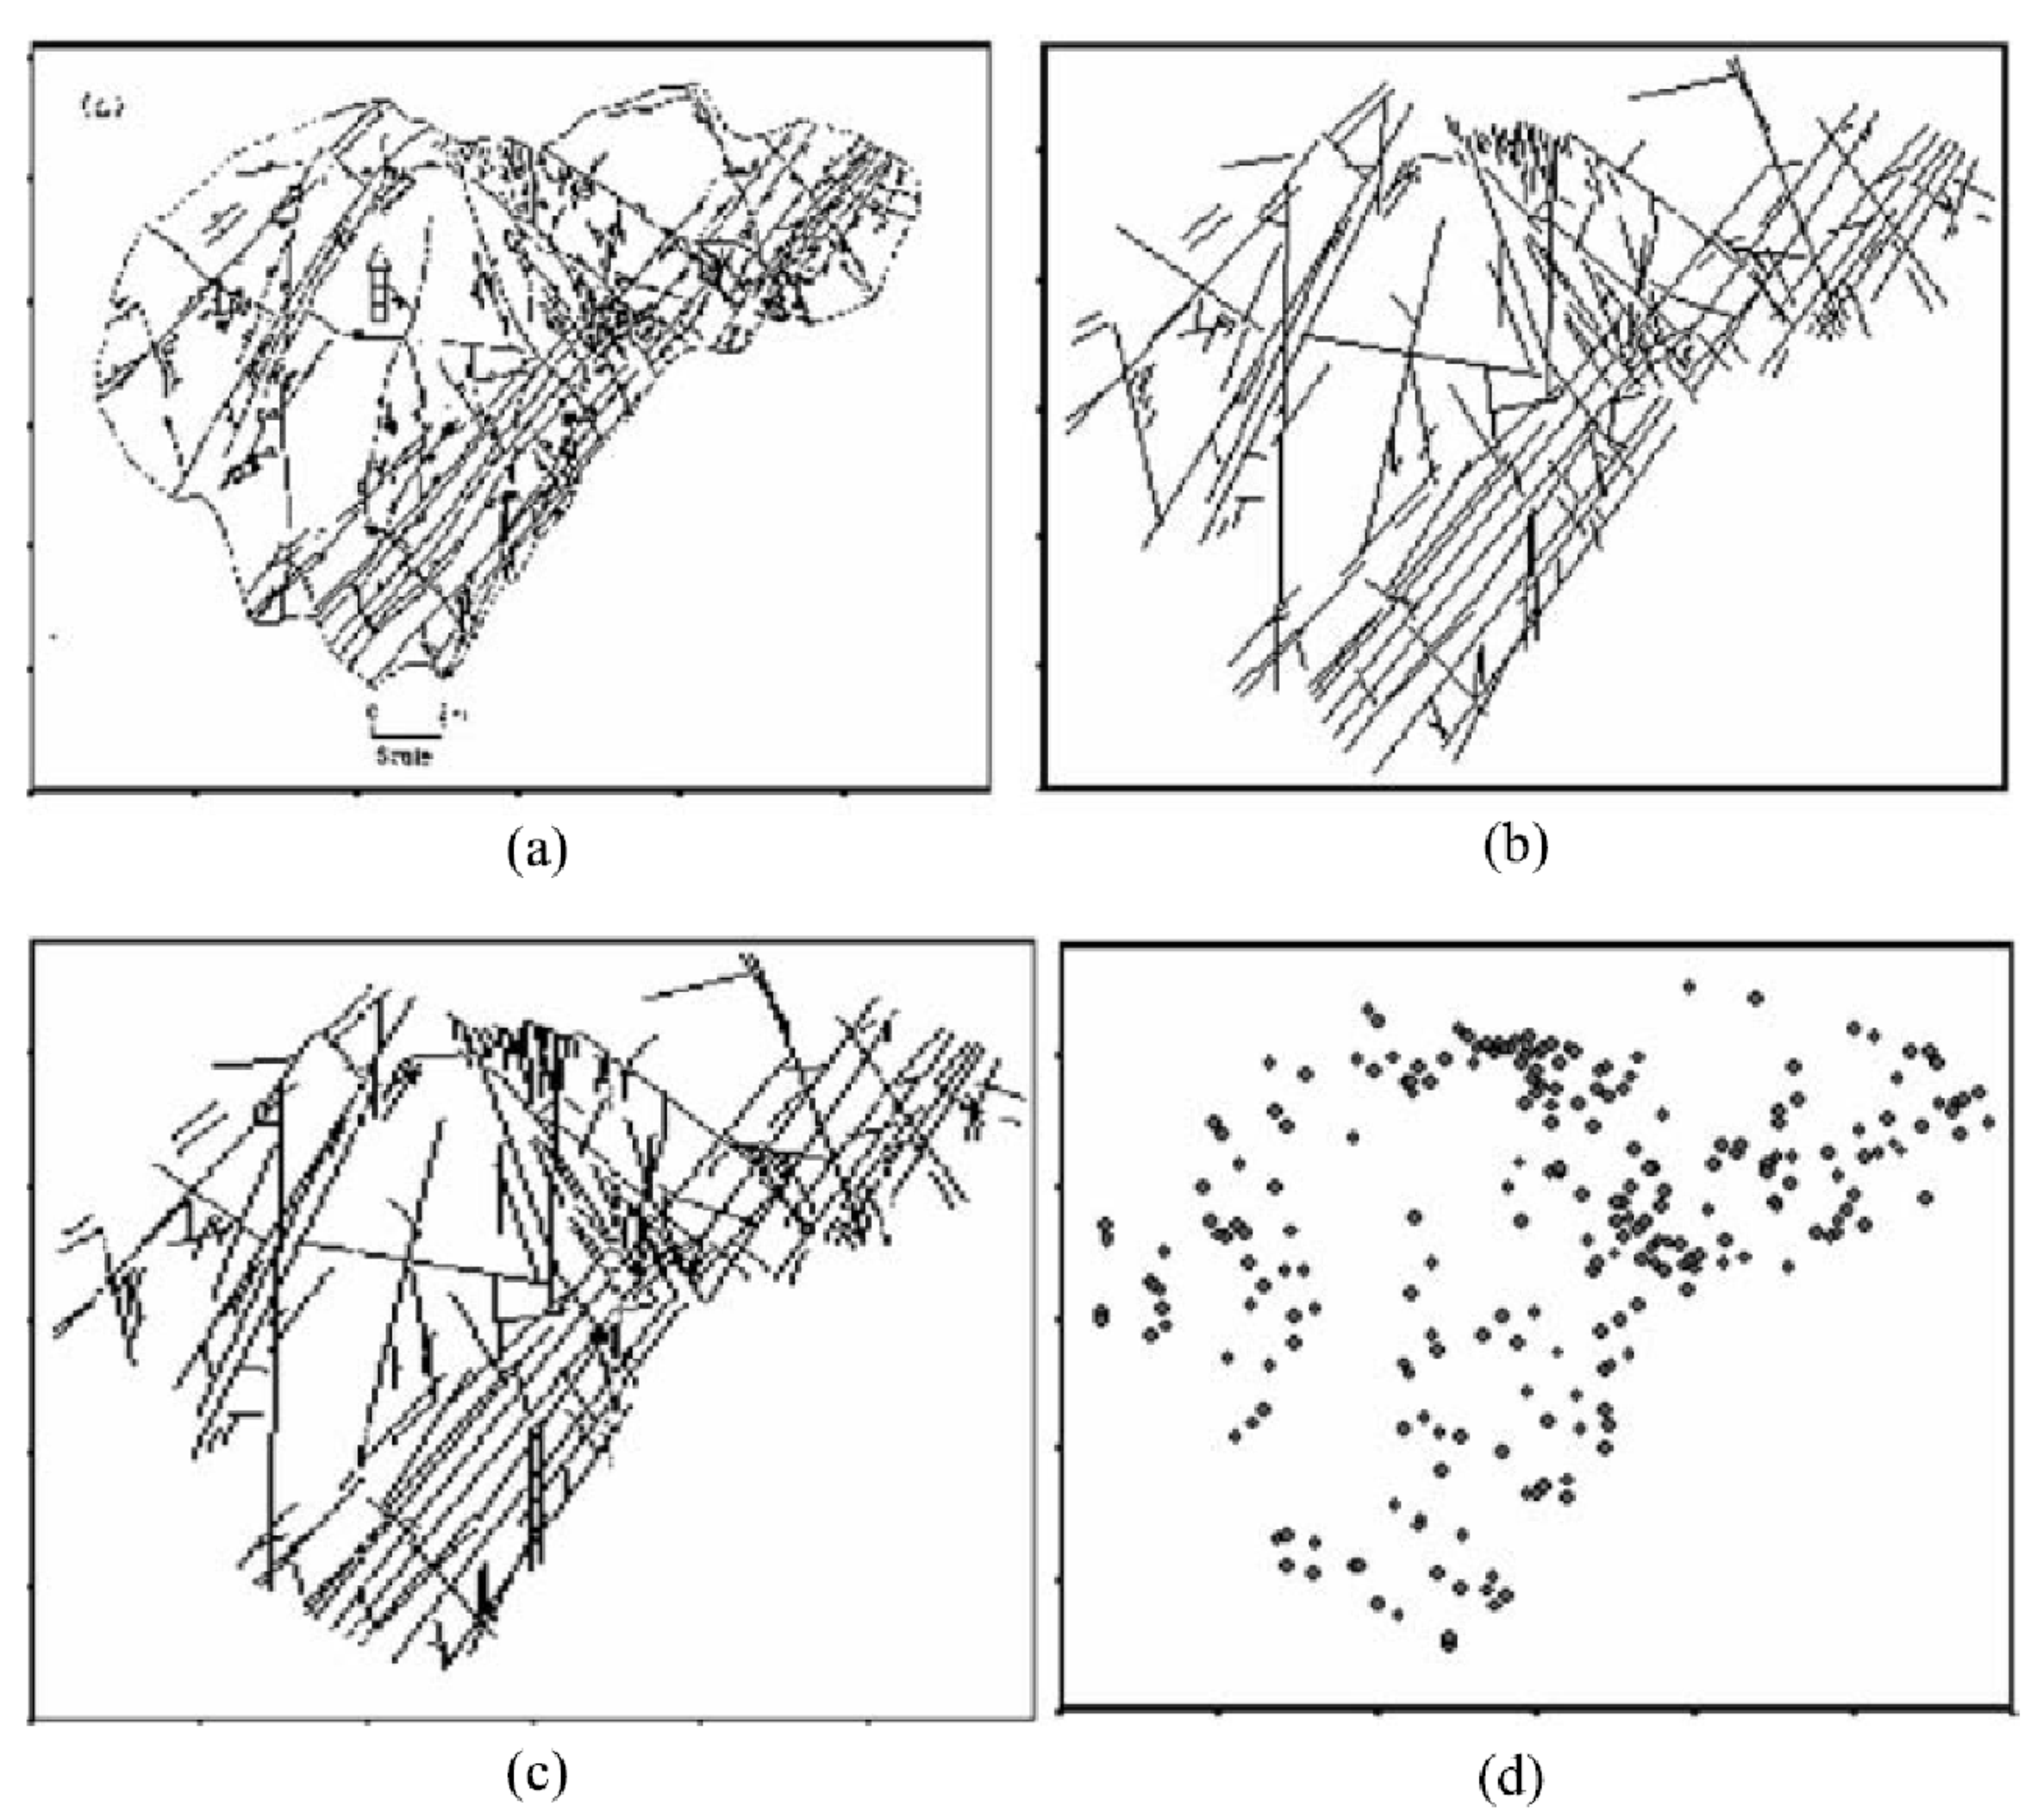
\includegraphics[width=0.8\textwidth]{fraxByIndicatorSim}
	\caption{a) fracturas; b) fracturas digitalizadas; c) Fracturas pixeladas; d) centroides de fracturas.}
	\label{f:fraxByIndicatorSim}
\end{figure}

La funci\'on indicador para la \autoref{f:fraxByIndicatorSim}-c) se define como

\begin{equation}
    \mathbbm{1}_{F}(x)=
\begin{cases}
	1,	& \text{si $x \in F$;}\\
	0,	& \text{en otro caso.}
\end{cases}
\label{e:indicatorFunc}
\end{equation}

\noindent
donde $F$ representa un conjunto, en este caso, el conjunto aleatorio de las fracturas "pixeladas". Por lo tanto, la simulaci\'on (no condicionada) puede ser realizada con el m\'etodo Gaussiano truncado, el cual a su vez utiliza variogramas. Los resultados de la modelaci\'on con este m\'etodo se muestran en la \autoref{f:fraxByIndicatorSimVario}.

\begin{figure}[H] 
	\centering
	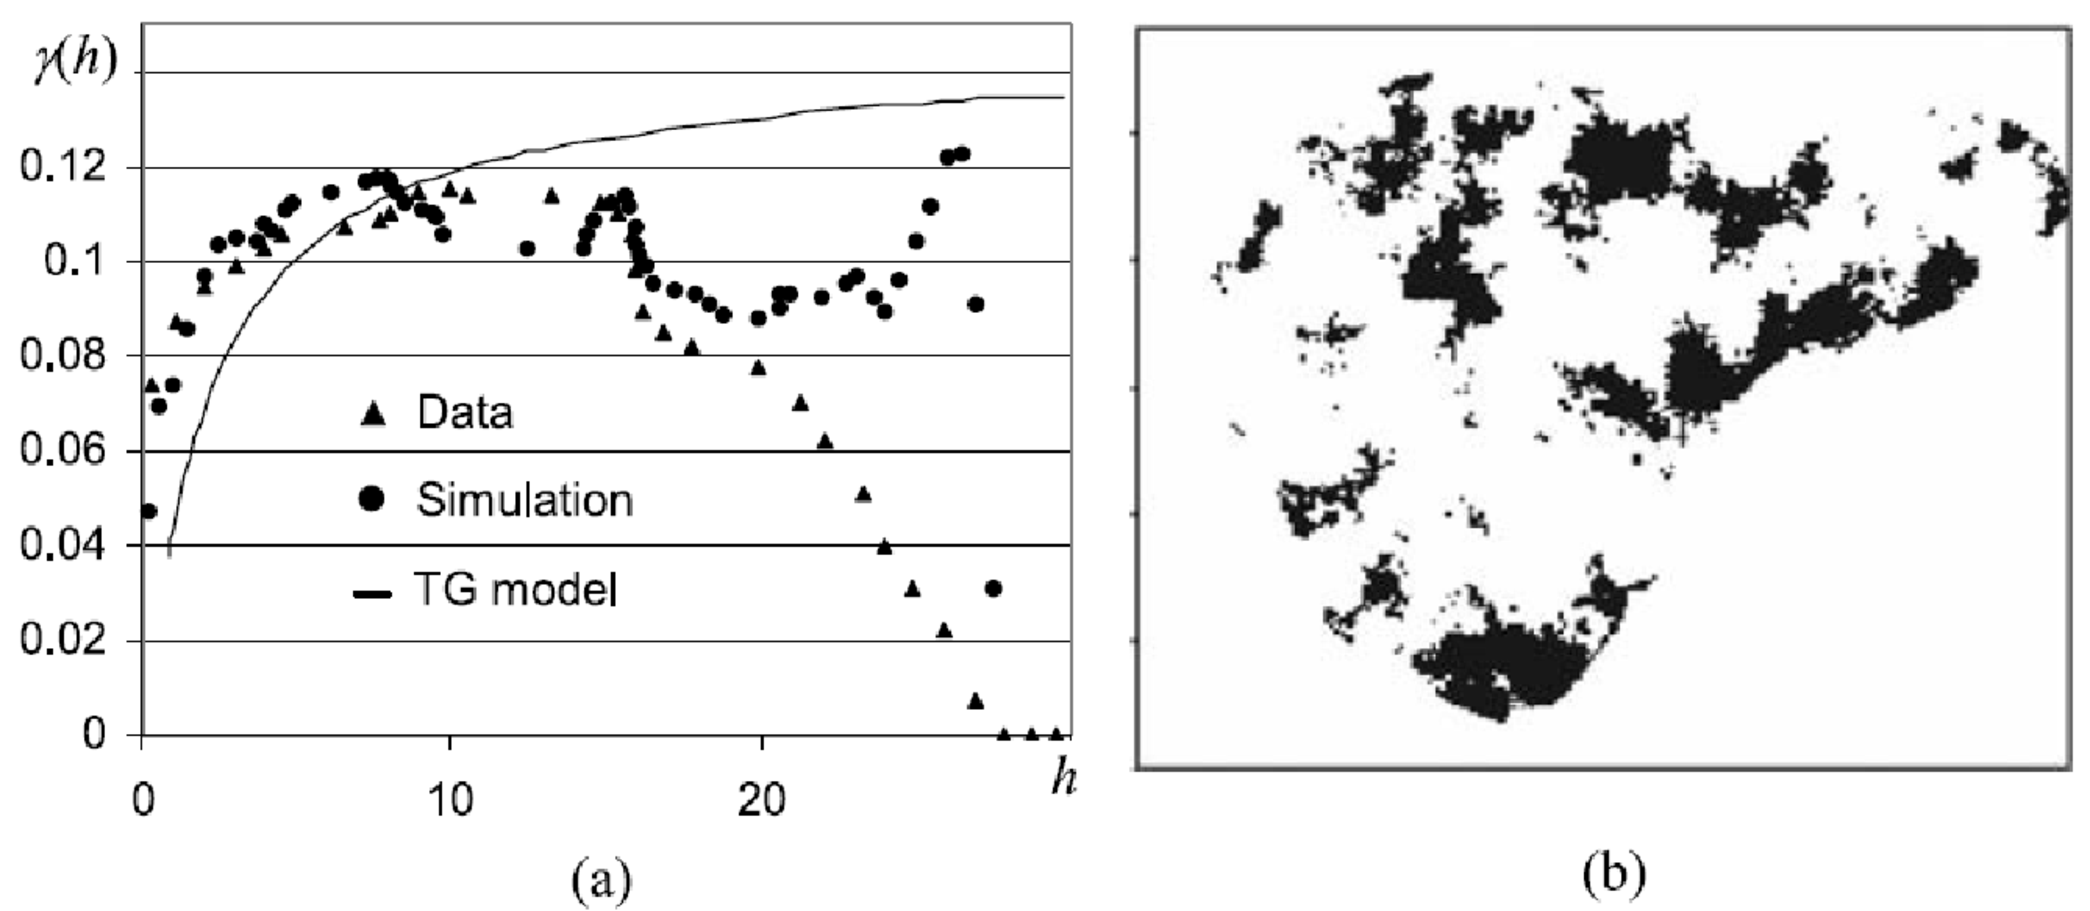
\includegraphics[width=0.8\textwidth, keepaspectratio = TRUE]{fraxByIndicatorSimVario}
        \caption{a) Variograma; b) Simulaci\'on. Modificada de la Fig. 2 de \citet{dowd_comparison_2007}}.
	\label{f:fraxByIndicatorSimVario}
\end{figure}

Aunque el modelo de variograma es reproducido razonablemente bien, la imagen simulada difiere considerablemente de la imagen original. Este ejemplo muestra que reproducir el primer orden y \'ordenes superiores de un campo aleatorio no necesariamente reproduce un proceso aleatorio.


\subsection{Modelo con geoestad\'istica multi-punto}

Utilizando el contexto de la geoestad\'istica convencional, el uso de s\'olo el primer y segundo momento es claramente insuficiente para simular las complejas estructuras de una red de fracturas. Utilizando las estad\'isticas de orden superior deber\'ia mejorar la simulaci\'on, aunque la reconstrucci\'on de todas las propiedades estoc\'asticas del campo aleatorio no se puede garantizar. La inferencia de orden superior en modelos estad\'isticos espaciales es dif\'icil, ya que se basan en las configuraciones espaciales en lugar de las distancias por pares y orientaciones simples usados en las formas tradicionales de la geoestad\'istica. Un enfoque consiste en utilizar la probabilidad condicional para una configuraci\'on particular para inferir experimentalmente el modelo espacial para describir el campo aleatorio.

Para una variable indicador, la probabilidad condicional es equivalente a la esperanza condicional de la configuraci\'on. La probabilidad condicional de que $\mathbbm{1}=1$, dado $n$ eventos $\mathbbm{1}(x) = 0$ \'o $1$ para $i = 1, \ldots, n$ se puede expresar como la suma de  t\'erminos de la siguiente manera:

\begin{equation}
	Prob
	\left\{
		\mathbbm{1} (x) = \mathbbm{1}(x_i), \qquad i = \{1,\ldots,n\}
		\\
		= \lambda_0 +
		\sum_{i=1}^n \lambda_i^{(1)} \mathbbm{1}(x_i) +
		\sum_{i=1}^n \sum_{j > i}^n \lambda_{ij}^{(2)}
		\mathbbm{1}(x_i) \mathbbm{1}(x_j) + \cdots
	\right\}
	\label{e:multiplePointG}
\end{equation}
	 	
Donde $\lambda_{\dots}^{()}$ son los $2^n+1$ coeficientes obtenidos por un sistema de Kriging simples extendidos. Los primeros $n+1$ t\'erminos se pueden resolver por Kriging (geoestad\'istica a dos puntos) y los otros t\'erminos describen el enfoque multi-punto de orden 3 al $n$.

Cuando se ha inferido la probabilidad condicional de la \autoref{e:multiplePointG}, $\mathbbm{1}(x)$ puede ser simulada mediante muestro Monte Carlo. Generalmente, la inferencia se basa en realizaciones de la variable aleatoria, a las cuales se les conoce como im\'agenes de entrenamiento. Estas im\'agenes de entrenamiento pueden ser datos o postulados en base a la experiencia. La simulaci\'on secuencial de $\mathbbm{1}(x)$ depende del n\'umero $n$ de datos indicadores, $\mathbbm{1}(x_i)$, m\'as cercanos a cada nodo $x$.

En la \autoref{f:fraxByMultiPoint} se muestran los resultados para diferentes valores de $n$. Estas simulaciones muestran la importancia de este  par\'ametro en la estad\'istica multi-punto. La selecci\'on de $n$ depende lo complejo de las estructuras a simular. En el ejemplo que aqu\'i se muestra se puede concluir que valores $n \le 12$ son inadecuados para describir el sistema de fracturas en cuesti\'on.

\begin{figure} 
	\centering
	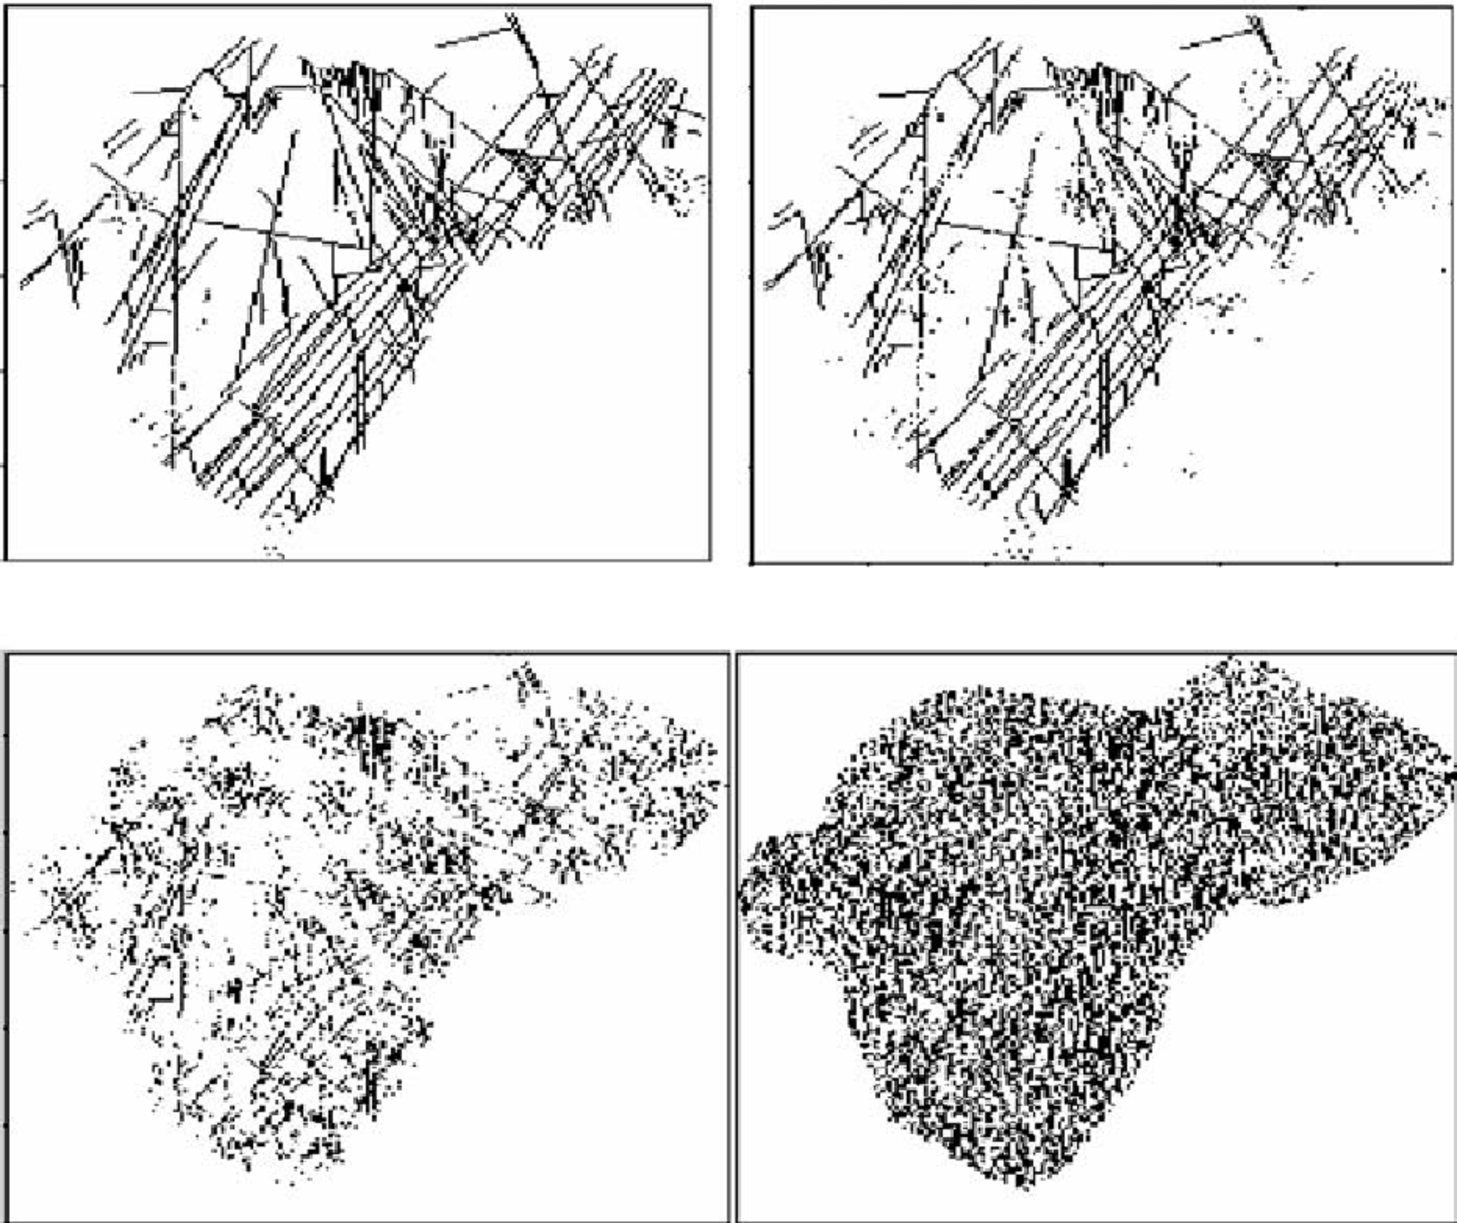
\includegraphics[width=0.8\textwidth, keepaspectratio = TRUE]{fraxByMultiPoint}
	\caption{Simulaciones basadas en la geoestad\'istica multi-punto.}
	\label{f:fraxByMultiPoint}
\end{figure}


\begin{table}
	\centering
\begin{tabular}{|l|c|c|}
\hline
$n$ & Pixeles negros (\%) & Posici\'on en la \autoref{f:fraxByMultiPoint} \\
\hline
\hline
20 & 19.63 & Superior izquierda\\ \hline
16 & 19.26 & Superior derecha\\ \hline
12 & 20.88 & Inferior izquierda\\ \hline  
8  & 43.97 & Inferior derecha\\ \hline
\end{tabular}
\caption{Valores de porcentajes de pixeles negros para los resultados en la \autoref{f:fraxByMultiPoint}.}
\end{table}

\subsection{Modelos booleanos}

Debido a la complejidad de las fracturas y m\'as a\'un de los sistemas de fracturas, no es viable modelarlas con demasiada precisi\'on. Por ejemplo, el simple hecho de intentar modelar las caras de las fracturas es computacionalmente lento. Si el objetivo buscado es la simulaci\'on de flujo, este \'ultimo puede tomar mucho m\'as tiempo si se considera la rugosidad de la fractura. En muchos de los casos, la rugosidad de estas superficies puede ser auto-af\'in, es decir tener propiedades fractales \citep[ch. 4]{adler_fractures_1999}.

Cuando se desea modelar un sistema de fracturas en alg\'un yacimiento, el enfoque del p\'arrafo anterior se torna imposible de implementar. Un enfoque m\'as viable es simplificar la geometr\'ia de las fracturas. Por ejemplo, se puede suponer que las caras son planos (\autoref{f:parallelPlates}), modelo conocido como de placas paralelas \citep{dietrich_flow_2005}.

\begin{figure}[H]
	\centering
	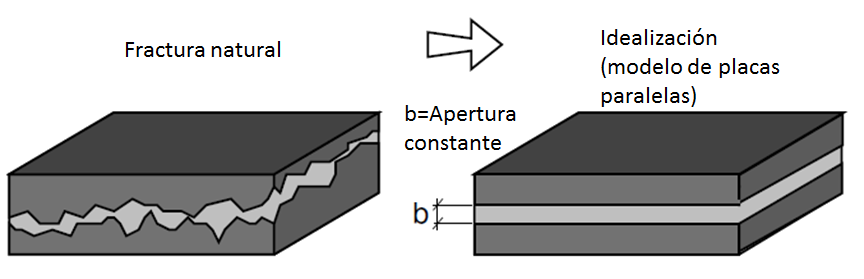
\includegraphics[width=0.7\textwidth]{parallelPlates}
	\caption{Modelado de una fractura. Izquierda: fractura real; derecha: su modelo de placas paralelas (Modificada de la Fig. 2.11 de \citeauthor{dietrich_flow_2005}, \citeyear{dietrich_flow_2005}).}
	\label{f:parallelPlates}
\end{figure}

Con el enfoque de \cite{dietrich_flow_2005}, se supone que las fracturas son discretas y simplificadas. Los modelos m\'as usuales para representar sistemas de fracturas en medios porosos en general y en particular en la modelaci\'on de Yacimientos Naturalmente Fracturados (YNF) son los modelos de Redes de Fracturas Discretas (DFN). Este tipo de modelos nos proporcionan el n\'umero de fracturas en determinado volumen con longitudes y orientaciones dadas. Estos modelos consideran a una fractura como un ente geom\'etrico simplificado, usualmente segmentos rectil\'ineos, paralelogramos y elipses en 2D, y pol\'igonos, paralelep\'ipedos y elipsoides en 3D. Por lo que una fractura discreta puede ser caracterizada por su longitud, apertura, orientaci\'on, etc. 

El m\'etodo estoc\'astico de simulaci\'on de fracturas discretas est\'a basado en el modelo booleano, el cual a su vez se construye a partir de procesos puntuales de Poisson que generan los centros geom\'etricos de los objetos que representan a las fracturas. Aqu\'i por objeto se est\'a considerando a los entes geom\'etricos que representan a las fracturas. Los objetos no son determin\'isticos, son aleatorios, es decir \'estos son generados estoc\'asticamente, por lo que sus caracter\'isticas geom\'etricas est\'an dadas por funciones de distribuci\'on de probabilidad.

La aplicaci\'on de los modelos booleanos no solamente se restringe a la generaci\'on de las redes de fracturas si no tambi\'en dentro de la teor\'ia de percolaci\'on continua. Esta teor\'ia cuantifica la probabilidad de que las fracturas generadas est\'en conectados y que ellas formen una trayectoria entre dos ubicaciones especiales dadas. En la tesis de \citet{ayala-garcia_estimacion_2014} se muestran algunos casos de percolaci\'on utilizando redes de fracturas similares, mas no iguales, a las que se trabajaron en esta tesis.

Dado que \'este es el enfoque computacionalmente m\'as viable para la modelaci\'on de fracturas en un yacimiento, es el que se adopt\'o en este trabado doctoral. En el siguiente cap\'itulo se explica m\'as la teor\'ia de los modelos booleanos. Por lo pronto diremos que la idea intuitiva es la de objetos simplificados aleatoriamente colocados en el espacio. La palabra aleatoria se utiliza en un sentido probabil\'istico y no significa que est\'en uniformemente distribuidos.


	\chapter{Modelos booleanos basados en objetos estoc\'asticos}
\label{ch3:booleanModels}

La presente revisi\'on se basa principalmente en el libro de \citet{lantuejoul_geostatistical_2002} pero se explican algunos conceptos mas detalladamente.

Los modelos booleanos, aunque simples en la idea intuitiva detr\'as de las matem\'aticas requieren otros ingredientes a\'un m\'as esenciales.
En particular, primero se presenta una breve rese\~na de la teor\'ia de procesos puntuales. Posteriormente se definen los modelos booleanos. Para la simulacion de dichos modelos son necesarios las bases te\'oricas presentadas en las dos secciones antes de la secci\'on de simulaci\'on y en la \'ultima secci\'on se presenta un caso teoricamente importante.

\section{Procesos puntuales}

Un proceso puntual aleatorio es un modelo estoc\'astico \citep{lantuejoul_geostatistical_2002} en el cual cada realizaci\'on est\'a formada por un n\'umero finito o contable de puntos en $\mathbb{R}^d$.

Aunque los elementos de un proceso puntual son muy b\'asicos, estos procesos pueden formar estructuras complicadas. La \autoref{f:pointProc} muestra algunos ejemplos, pero existe una gran variedad de modelos. Adem\'as, en muchos fen\'omenos la simplificaci\'on de eventos espaciales a puntos es bastante adecuada. Por ejemplo, para modelar \'arboles en los bosques, epicentros de terremotos, estrellas en las galaxias, entre otros. Una raz\'on m\'as de la importancia de los procesos puntuales, es que ellos sirven de ingredientes para modelos m\'as complicados como en los que se enfoca esta tesis.

\DTLloaddb[noheader=false]{ppHom}{code/datasets/ppHom.csv}
\DTLloaddb[noheader=false]{ppInHom}{code/datasets/ppInHom.csv}
\DTLloaddb[noheader=false]{ppCluster}{code/datasets/ppCluster.csv}
\begin{figure}
	\centering
\begin{tikzpicture}[scale=4.5]
        \draw[color=lightgray, thick, fill=white] (-0.03,-0.03) rectangle (1.03,1.03);
	\DTLforeach*{ppHom}{\x=x, \y=y}{\path[fill=blue] (\x,\y) circle (0.015);}
\end{tikzpicture}
\hfill
\begin{tikzpicture}[scale=4.5]
        \draw[color=lightgray, thick, fill=white] (-0.03,-0.03) rectangle (1.03,1.03);
	\DTLforeach*{ppInHom}{\x=x, \y=y}{\path[fill=blue] (\x,\y) circle (0.015);}
\end{tikzpicture}
\hfill
\begin{tikzpicture}[scale=4.5]
        \draw[color=lightgray, thick, fill=white] (-0.03,-0.03) rectangle (1.03,1.03);
	\DTLforeach*{ppCluster}{\x=x, \y=y}{\path[fill=blue] (\x,\y) circle (0.015);}
\end{tikzpicture}
	\caption{Ejemplos de procesos puntuales. a) Caso Homog\'eneo, b) Intensidad no uniforme c) Proceso de conglomerados.}
%\protect\hypertarget{_Ref405932721}{}{}Figura 13. 
	\label{f:pointProc}
\end{figure}

%\begin{figure}[H]
    %\centering
    %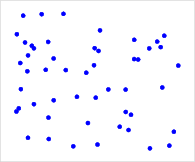
\includegraphics{pointProcessHom} \hfill
    %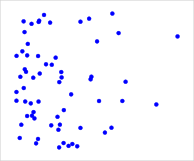
\includegraphics{pointProcessInhom} \hfill
    %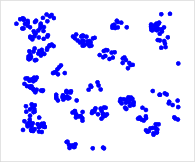
\includegraphics{pointProcessCluster}
    %\caption{Name}
    %\label{fig:pointProcPGF}
%\end{figure}


En un proceso puntual \textit{localmente finito} el n\'umero de puntos dentro de cualquier conjunto compacto (cerrado y acotado) es casi seguramente finito.
En este caso es conveniente describir las propiedades estad\'isticas del proceso puntual mediante un conteo del n\'umero de puntos dentro de subconjuntos del espacio.
Sea $N(B)$ el n\'umero aleatorio de puntos dentro del conjunto $B$, denominado el funcional que cuenta. $B$ es un elemento de $\mathcal{B}_0$, el conjunto de los Borelianos acotados.

La distribuci\'on espacial de un \textbf{proceso homog\'eneo de Poisson} con intensidad $\theta$ est\'a caracterizado por las siguientes propiedades:

\begin{enumerate}
	\item Si $A \in \mathcal{B}_0$, entonces el n\'umero de puntos dentro de $A$, $N(A)$, es una variable aleatoria de Poisson con par\'ametro $\lambda \|A\|$ donde $\|A\|$ es el $d$-volumen de $A$
		\begin{equation*}
			P\{N(A) = n\} =
			exp\{-\lambda \|A\|\}
			\frac{[\lambda \|A\|]^n}{n!}
		\end{equation*}
	\item Si $(A_i, i \in I)$ es una familia finita de elementos disjuntos de $\mathcal{B}_0$, entonces las variables aleatorias $N(A_i), i \in I)$ son mutuamente independientes.
\end{enumerate}

Dado que el valor medio de la distribuci\'on de Poisson es igual a su par\'ametro $\lambda$, la media del n\'umero de puntos sobre $A$ es igual a $\lambda \|A\|$. En particular, $\lambda$ es la media del n\'umero de puntos por unidad de $d$-volumen. Si se requiere simular una cantidad exacta de puntos, entonces $\|A\| / n = <~\lambda~>$ da un valor (medio $<\cdot>$) aproximado de la intensidad. Sin embargo, esta intensidad calculada no es la \'unica porque existe un conjunto no-numerable de valores de intensidad que pueden producir el mismo $n$.

El siguiente teorema, cuya demostraci\'on se puede encontrar en \cite[p. 121]{lantuejoul_geostatistical_2002}, muestra que los puntos de un proceso puntual homog\'eneo de Poisson son independientes y con ubicaci\'on totalmente aleatoria.

Sea $A \in \mathcal{B}_0$. Si $N(A)=n$, los $n$ puntos son independientes y uniformemente distribuidos en $A$.

Este teorema permite un algoritmo simple para simular un proceso puntual de Poisson en una regi\'on A.

\begin{enumerate}
	\item Inicialice el conjunto $X = \emptyset$,
	\item Obtenga cu\'antos puntos van a ser simulados al muestrear $n \sim Poisson(\theta \|A\|)$,
	\item si $n > 0$, para $i=1, \ldots,n$ genere $x_i \sim Unif(A)$,
	\item Los puntos $x_i \in \mathbb{R}^d$ pertenecientes a la realizaci\'on del proceso puntual son $X=\{x_1, \dots, x_n\}$.
\end{enumerate}

Computacionalmente, $X$ puede ser un arreglo bidimensional de $n \times d$, $n$ renglones por $d$ columnas. Aunque este algoritmo es computacionalmente r\'apido, se puede hacer m\'as eficiente si se toma en cuenta el orden de este arreglo ($n \times d$ \'o $d \times n$); dependiendo del paradigma en la memoria: row-major vs column-major \citep{karniadakis_parallel_2003,matloff_parallel_2016}.

El lenguaje de programaci\'on utilizado para desarrollar esta tesis fue \verb|R| ya que fue dise\~nado para desarrollos estad\'isticos y hay varios paquetes ya disponibles en su repositorio que complementan a este trabajo. A lo largo de esta tesis se referir\'a una funci\'on de alg\'un paquete de \verb|R| escribi\'endola con la siguiente sintaxis \verb|paquete::funcion|.

El algoritmo para generar realizaciones de un proceso puntual de Poisson est\'a computacionalmente implementado en la funci\'on \verb|spatstat::rpoint| del software \verb|R|. Si ya se sabe el valor de $n$, entonces la funci\'on que simula los puntos, dentro del mismo software, se llama \verb|spatstat::runifpoint|.

Los mejores ejemplos para la metodolog\'ia mostrada en esta tesis se obtuvieron con procesos puntuales homog\'eneos en los cuales $\lambda$ es constante. Otros modelos comunes son cuando $\lambda$ var\'ia espacialmente (Proceso puntual de Poisson no homog\'eneo) y cuando la intensidad espacial es una funci\'on aleatoria (Proceso de Cox).

\section{Construcci\'on del modelo booleano}

Se necesitan dos ingredientes b\'asicos e independientes para la construcci\'on de un modelo booleano en $\mathbb{R}^d$:

\begin{enumerate}
\item Un conjunto de \textit{semillas}, esto es, un proceso puntual de Poisson $\mathcal{P}$ con funci\'on de intensidad $\theta=(\theta(x),\ x\in\mathbb{R}^d)$.
    \item Una familia $(A(x),x\in\mathbb{R}^d)$ de subconjuntos de $\mathbb{R}^d$ compactos, no vac\'ios, aleatorios e independientes. Al subconjunto $A(x)$ se le llama el \textit{objeto implantado en} $x$ y su funcional que pega se denota por $\mathcal{T}_x$.
\end{enumerate}

De este modo, un modelo booleano $X$ es la \textit{uni\'on de todos los objetos implantados en las semillas Poisson}

\[X=\bigcup_{x\in\mathcal{P}}A(x)\]

La apariencia de una realizaci\'on del modelo depende en gran medida de la forma que tengan los objetos. \'Estos pueden ser, por ejemplo, segmentos de recta, discos, pol\'igonos, etc\'etera. En la \autoref{f:boolEx} se muestran dos realizaciones de modelos booleanos. En el primer caso se muestra un conjunto de c\'irculos --los objetos-- implantados sobre semillas de Poisson homog\'eneamente distribuidas. Y en el segundo caso se muestra otra realizaci\'on en el cual los objetos son segmentos rectil\'ineos.

\begin{figure}[H]
	\centering
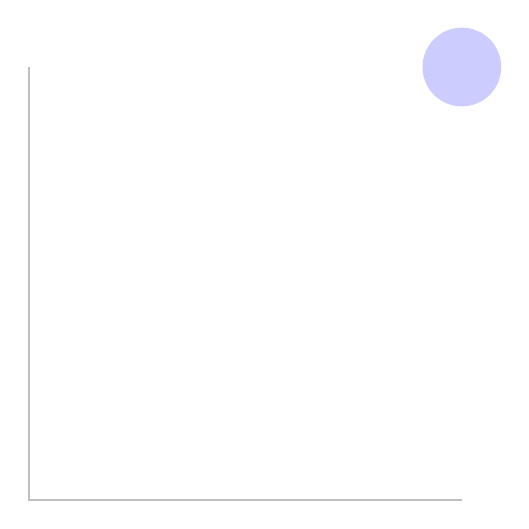
\begin{tikzpicture}[scale=5]
	\draw[lightgray, thick] (-0.1,1) -- (-0.1,-0.1) -- (1,-0.1);
\DTLforeach*{ppHom}{\x=x, \y=y}{\path [fill=blue, fill opacity=0.2] (\x,\y) circle (0.1cm);}
\end{tikzpicture}
%\hfill
%\begin{pgfpicture}% example from tikz manual 3.0.1
	%\pgfmathdeclarerandomlist{color}{{red}{blue}{green}{yellow}{white}}
	%\foreach \a in {1,...,50}{
		%\pgfmathrandominteger{\x}{1}{85}
		%\pgfmathrandominteger{\y}{1}{85}
		%\pgfmathrandominteger{\r}{5}{10}
		%\pgfmathrandomitem{\c}{color}
		%\pgfpathcircle{\pgfpoint{+\x pt}{+\y pt}}{+\r pt}
		%\color{\c!40!white}
		%\pgfsetstrokecolor{\c!80!black}
		%\pgfusepath{stroke, fill}
	%}
%\end{pgfpicture}
\qquad
\qquad
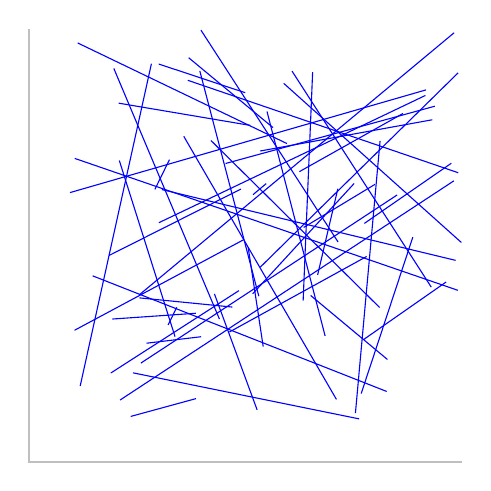
\begin{tikzpicture}[scale=5]
	\draw[lightgray, thick] (-0.1,1) -- (-0.1,-0.1) -- (1,-0.1);
	%\draw[lightgray, thick] (0,1) -- (0,0) -- (1,0);
	\foreach \x in {1,2,...,50}{
	\draw[blue] (rnd,rnd) -- (rnd,rnd);}
\end{tikzpicture}
\caption{Ejemplos de modelos booleanos cuyos objetos son (a) c\'irculos;
%b) modelo booleano con m\'as atributos denotdaos por el color y el tama\~no de  los objetos circulares;
b) Segmentos lineales.}
\label{f:boolEx}
\end{figure}

Ya que un modelo booleano es posiblemente la uni\'on de una infinidad de objetos, no existe garant\'ia de que sea cerrado. Este ser\'a ciertamente el caso si para cada punto $x\in\mathbb{R}^d$ existe una vecindad a la cual s\'olo le pega una cantidad finita de objetos (casi seguramente), y en particular si la poblaci\'on de objetos $(A(x),x\in\mathcal{P})$ es de orden finito. Espec\'ificamente, sea $N(K)$ el n\'umero de objetos que le pegan al compacto $K$. Entonces

\[N(K)=\sum_{x\in\mathcal{P}}\mathbbm{1}_{K\cap A(x)\neq\emptyset}.\]

Un c\'alculo sencillo muestra que la media de $N(K)$ es

\[\vartheta(K)=\int_{\mathbb{R}^d}\theta(x)\mathcal{T}_x(K)dx\ \leq\ \infty.\]

Se dice que un modelo booleano es de \textbf{orden finito} si $\vartheta(K)<\infty\ \forall\ K\in\mathcal{K}$. A lo largo de este texto se supondr\'a que los modelos booleanos considerados son de orden finito.

\section{El funcional que evita (avoiding functional) del modelo booleano}

Comencemos determinando la distribuci\'on del n\'umero de objetos que intersectan al subconjunto compacto $K$.

Se tendr\'a que $N(K)$ es una variable aleatoria Poisson con media $\vartheta(K)$: Para cada $D\in\mathcal(K)$ consideremos el n\'umero $N_D(K)$ de objetos implantados en $D$ que le pegan a $K$.

\[N_D(K)=\sum_{x\in\mathcal{P}\cap D}\mathbbm{1}_{K\cap A(x)\neq\emptyset}.\]

Por definici\'on, el n\'umero de puntos en $\mathcal{P}\cap D$ sigue una distribuci\'on Poisson con media

\[\theta(D)=\int_D \theta(x)dx.\]

Supongamos que este n\'umero es igual a $n$. De acuerdo a las propiedades de un proceso puntual de Poisson estos puntos est\'an distribuidos de manera uniforme e independiente sobre $D$, con funci\'on de densidad de probabilidad $\frac{\theta(\cdot)}{\theta(D)}$. M\'as a\'un, un objeto implantado en $x$ le pega a $D$ con probabilidad $\mathcal{T}_x(K)$ y lo evita con la probabilidad complementaria $1-\mathcal{T}_x(K)$. En consecuencia, la funci\'on generadora de $N_D(K)$ es

\[\mathbb{E}\left\{s^{N_D(K)}\right\}=\sum_{n=0}^\infty e^{-\theta(D)}\frac{\theta(D)^n}{n!}\left(\int_D\frac{\theta(x)}{\theta(D)}[(1+(s-1)\mathcal{T}_x(K)]dx\right)^n,\]

donde $0\leq s\leq 1$, y al sumar se tiene que

\[\mathbb{E}\left\{s^{N_D(K)}\right\}=\exp\left\{(s-1)\int_D\theta(x)\mathcal{T}_x(K)dx\right\}.\]

Para extender este resultado a todo el espacio, sea $(D_n,n\in\mathbb{N})$ una sucesi\'on creciente de compactos que cubren a $\mathbb{R}^d$. Entonces $(N_{D_n}(K),n\in\mathbb{N})$ tambi\'en es una sucesi\'on creciente y converge casi seguramente a $N(K)$. En consecuencia

\[\mathbb{E}\left\{s^{N(K)}\right\}=\lim_{n\rightarrow\infty}\mathbb{E}\left\{s^{N_{D_n}(K)}\right\}=exp\left\{(s-1)\int_{\mathbb{R}^d}\theta(x)\mathcal{T}_x(K)dx\right\}.\]

Esta \'ultima expresi\'on se reconoce como la funci\'on generadora de una distribuci\'on Poisson con media $\vartheta(K)$.

Ya que $\mathbb{P}\{X\cap K=\emptyset\}=\mathbb{P}\{N(K)=0\}$, deducimos que el funcional que evita del modelo booleano es

\[\mathbb{P}\{X\cap K=\emptyset\}=e^{-\vartheta(K)},\ \ K\in\mathcal{K}.\]

\section{Propiedades de estabilidad}

Para poder explorar las propiedades de estabilidad del modelo booleano es necesario echar mano de conceptos b\'asicos de morfolog\'ia, a saber, el concepto de \textit{dilataci\'on}.

 Dados $x\in\mathbb{R}^d$ y $A\subset\mathbb{R}^d$, $A_x$ denota al conjunto obtenido al trasladar $A$ por $x$. Si $B$ es un subconjunto de $\mathbb{R}^d$ entonces la \textit{suma de Minkowski} de $A$ y $B$ es

\[A\oplus B = \bigcup_{y\in B}A_y.\]

Decimos entonces que el punto $x$ pertenece al conjunto $A$ \textit{dilatado} por $B$ si $B_x$ le pega a $A$ (es decir, si $B_x\cap A\neq\emptyset$.

Por otra parte, necesitaremos tambi\'en el concepto de $i$-planos, los cuales son espacios afines de dimensi\'on $i$. [Un espacio af\'in es un espacio vectorial sin origen].

Las propiedades b\'asicas de estabilidad de un modelo booleano son:

\begin{itemize}
	\item La uni\'on de dos modelos booleanos independientes es un modelo booleano.
	\item Un modelo booleano dilatado por un subconjunto compacto no vac\'io de $\mathbb{R}^d$ es un modelo booleano.
	\item La intersecci\'on de un modelo booleano con un subconjunto compacto de $\mathbb{R}^d$ es un modelo booleano.
	\item La intersecci\'on de un modelo booleano y un $i$-plano es un modelo booleano.
\end{itemize}

A continuaci\'on, se proporcionan argumentos para justificar estas afirmaciones:

Sean $X'$ y $X''$ dos modelos booleanos independientes con funciones de identidad $\theta'$ y $\theta''$, y funcionales que pegan $\mathcal{T}'$ y $\mathcal{T}''$. Debido a la independencia se tiene que

\[\begin{array}{ccl}
\mathbb{P}\{(X'\cup X'')\cap K=\emptyset\}&=&\mathbb{P}\{X'\cap K=\emptyset\}\mathbb{P}\{X''\cap K=\emptyset\}\\
&&\\
&=&\exp\left\{-\int_{\mathbb{R}^d}\theta'(x)\mathcal{T}'_x(K)+\theta''(x)\mathcal{T}_x''(K)dx\right\}\\
&&\\
&=&\exp\left\{-\int_{\mathbb{R} ^d}\theta(x)\mathcal{T}_x(K)dx\right\}
\end{array}\]

donde $\theta=\theta'+\theta''$ y $\mathcal{T}_x$ queda definido como

\[\mathcal{T}_x(K)=\frac{\theta'(x)}{\theta'(x)+\theta''(x)}\mathcal{T}'_x(K)+\frac{\theta''(x)}{\theta'(x)+\theta''(x)}\mathcal{T}''_x(K),\ \ K\in\mathcal{K}.\]

Este es el funcional que pega de un objeto aleatorio igual a $A'(x)$ con probabilidad $\frac{\theta'(x)}{\theta'(x)+\theta''(x)}$, e igual a $A''(x)$ con probabilidad complementaria $\frac{\theta''(x)}{\theta'(x)+\theta''(x)}$. Este hecho prueba la primera propiedad.

Ahora bien, sea $D$ un subconjunto de $\mathbb{R}$ compacto y no vac\'io. La segunda propiedad es consecuencia directa de la distributividad de la suma de Minkowski sobre la uni\'on de conjuntos:

\[X\oplus D=\bigcup_{x\in\mathcal{P}}A(x)\oplus D.\]

De este modo, la dilataci\'on de un modelo booleano vuelve a ser la uni\'on de objetos aleatorios implantados en las semillas determinadas por $\mathcal{P}$, lo cual determina un nuevo modelo booleano. La diferencia es que en lugar de tener los objetos aleatorios originales $A(x)$, se tienen los objetos aleatorios dilatados $A(x)\oplus D$.

En cuanto a la tercera propiedad, podemos escribir simplemente $X\cap D=\bigcup_{x\in\mathcal{P}}A(x)\cap D$. Sin embargo, esta f\'ormula es dif\'icil de interpretar ya que los objetos $A(x)\cap D$ ser\'an casi seguramente vac\'ios. En cambio, consideraremos la siguiente expresi\'on:

\[\begin{array}{ccl}
\mathbb{P}\{(X\cap D)\cap K=\emptyset\}&=&\mathbb{P}\{X\cap (D\cap K)=\emptyset\}\\
&&\\
&=&\exp\left\{-\int_\mathbb{R}^d\theta(x)\mathcal{T}_x(D\cap K)dx\right\}\\
&&\\
&=&\exp\left\{-\int_\mathbb{R}^d\mathcal{T}_x(D)\frac{\theta(x)\mathcal{T}_x(D\cap K)}{\mathcal{T}_x(D)}dx\right\}
\end{array}
.\]

Pero $\frac{\theta(x)\mathcal{T}_x(D\cap K)}{\mathcal{T}_x(D)}$ es el funcional que pega de $A(x)\cap D$, ya que este objeto es no vac\'io. En consecuencia, $X\cap D$ es un modelo booleano con funci\'on de intensidad $\theta\mathcal{T}(D)$ y funcional que pega $\frac{\theta\mathcal{T}(D\cap K)}{\mathcal{T}(D)}$.

Finalmente, sea $P$ un $i$-plano de $\mathbb{R}^d$. La \'ultima propiedad se puede deducir de la tercera tomando una sucesi\'on creciente de compactos no vac\'ios $(D_n,n\in\mathbb{N})$ que converja a $P$.

El modelo booleano es un caso especial de los modelos basados en objetos. Una primera extensi\'on consiste en reemplazar el proceso puntual de Poisson que especifica la localizaci\'on de los objetos a trav\'es de un proceso espacial de nacimiento y muerte (Preston, 1977; Stoyan et al., 1987). Tambi\'en es posible permitir dependencia entre los objetos. En ese caso, un objeto se inserta o se elimina dependiendo de una funci\'on de los objetos ya presentes (y no solamente el n\'umero de \'estos). Esto lleva al concepto de un proceso de vida y muerte de objetos en el espacio. Un ejemplo t\'ipico es el modelo de interacci\'on dos a dos considerado por Sylverseen y Omre (1994). La primera versi\'on de este modelo incluy\'o un n\'umero fijo de objetos, lo cual permit\'ia la simulaci\'on a trav\'es de un muestreo de Gibbs. Esta restricci\'on fue eliminada en un art\'iculo posterior (1997). Es posible extender el modelo de muchas otras maneras, como el proceso de saltos de Markov de objetos.


\section{Simulaci\'on del modelo booleano}

El problema entre manos es simular el modelo booleano en $D$, sujeto a las condiciones de que dos subconjuntos finitos $C_0$ y $C_1$ deben estar contenidos en $X^c$ y $X$, respectivamente. Este problema es importante en la industria petrolera. Los ingenieros petroleros requieren conocer la geometr\'ia del yacimiento para poder ejecutar programas de simulaci\'on de flujos. Un algoritmo desarrollado por Haldersen en 1983 fue notablemente mejorado por Chessa en 1995. Consiste en simular de manera independiente los cuerpos arenosos (los objetos) que intersecan los pozos y aquellos que no. Esta perspectiva dicot\'omica es posible gracias a las propiedades de independencia del proceso Poisson. La dificultad de esta estrategia es que la distribuci\'on de un objeto que interseca al pozo depende no solamente de d\'onde est\'e implantado, sino tambi\'en del n\'umero y la localizaci\'on de los pozos que interseca. Usualmente, el problema se vuelve intratable en cuanto este n\'umero es mayor a uno.

El algoritmo iterativo descrito a continuaci\'on fue dise\~nado a partir de comunicaciones privadas entre Matheron y Lantu\'ejoul en 1990. Posteriormente Gedler (1991) llevo a cabo el trabajo preliminar bajo la supervisi\'on de Lantu\'ejoul. Ya que este algoritmo de simulaci\'on condicional es una versi\'on modificada de un algoritmo de simulaci\'on no condicional (mediante la restricci\'on del kernel de transici\'on), se presenta primero el algoritmo de simulaci\'on no condicional.

Se discuti\'o anteriormente que $X\cap D$ es un modelo booleano con funci\'on de intensidad $\theta(\cdot)\mathcal{T}_x(D)$. De manera acorde, el n\'umero de objetos de $X\cap D$ es de distribuci\'on Poisson con media

\[\vartheta(D)=\int_{\mathbb{R}^d}\theta(x)\mathcal{T}_x(D)dx.\]

El funcional que pega de un objeto de $X\cap D$ implantado en $x$ es $\frac{\mathcal{T}_x(D\cap\cdot)}{\mathcal{T}_x}(D)$.

Un \textit{objeto t\'ipico} de $X\cap D$ es un objeto seleccionado uniformemente entre los objetos de $X\cap D$. Un objeto t\'ipico de $X\cap D$ se implanta de acuerdo a la funci\'on de densidad $\theta(\cdot)\mathcal{T}(D)$.  Su funcional que pega es

\[\mathcal{T}(K)=\int_{\mathbb{R}^d}\frac{\theta(x)\mathcal{T}_x(D)}{\vartheta(D)}\frac{\mathcal{T}_x(D\cap K)}{\mathcal{T}_x(D)}=\frac{1}{\vartheta(D)}\int_{\mathbb{R}^d}\theta(x)\mathcal{T}_x(D\cap K)dx\]
\vspace{0.1in}
Notemos que en particular $\mathcal{T}(D)=1$ y $\mathcal{T}(K)=0$ si $K$ es disjunto de $D$.

Por otra parte, $X\cap D$ tiene la misma distribuci\'on que una uni\'on de $N$ objetos t\'ipicos independientes, donde $N$ tiene distribuci\'on Poisson con media $\vartheta(D)$. Este hecho se prueba del siguiente modo: Sea $Y$ tal uni\'on. Su funcional que evita es

\[\begin{array}{ccl}\mathbb{P}\{Y\cap K=\emptyset\}&=&\sum_{n=0}^\infty e^{-\vartheta(D)}\frac{\vartheta(D)^n}{n!}[1-\mathcal{T}(K)]^n\\
&&\\
&=&exp\{-\vartheta(D)\mathcal{T}(K)\}\\
&&\\
&=&exp\left\{-\int_{\mathbb{R}^d}\theta(x)\mathcal{T}_x(D\cap K)dx\right\}
\end{array}\]

el cual resulta ser exactamente el funcional que evita de $X\cap D$.

En consecuencia, una simulaci\'on no condicional del modelo booleano se puede obtener utilizando el siguiente algoritmo:

\textbf{Algoritmo para el modelo booleano:}
\begin{enumerate}
\item Hacer $X=\emptyset$.
\item Generar $N\sim Poisson(\vartheta(D))$.
\item Si $N=0$, regresar $X$.
\item Generar un objeto t\'ipico $A\sim\mathcal{T}$.
\item Hacer $X=X\cup A$, $N=N-1$ e ir al paso 3.
\end{enumerate}

Este algoritmo requiere de la simulaci\'on de un objeto t\'ipico. El algoritmo est\'andar es:

\textbf{Algoritmo para el objeto t\'ipico}
\begin{enumerate}
\item Generar $X\sim \theta(\cdot)\mathcal{T}(D)$.
\item Generar $A\sim \frac{\mathcal{T}_x(D\cap\cdot)}{\mathcal{T}_x(D)}$.
\item Regresar $A$.
\end{enumerate}

Si resulta dif\'icil simular un objeto implantado en $x$ y pegarle a $D$ directamente, es posible emplear un algoritmo alternativo de rechazo.

\textbf{Algoritmo para el objeto t\'ipico (m\'etodo de rechazo)}
\begin{enumerate}
\item Generar $X\sim \theta(\cdot)\mathcal{T}(D)$.
\item Generar $A\sim \mathcal{T}_x$.
\item Si $A\cap D=\emptyset,$ ir al paso 2.
\item Regresar $A\cap D$.
\end{enumerate}

Finalmente, el primer algoritmo se modifica ligeramente para volverlo iterativo. Esto no presenta dificultad alguna ya que algoritmo de Metr\'opolis puede ser utilizado para simular una distribuci\'on Poisson. El siguiente algoritmo simula iterativamente un modelo Poisson. Espec\'ificamente, simula la poblaci\'on de objetos que constituye el modelo booleano. En este algoritmo el n\'umero de objetos de la poblaci\'on $\Phi$ se denota por $\#\Phi$.


\textbf{Algoritmo para objetos de un modelo booleano}

\begin{enumerate}
\item Hacer $\Phi=\emptyset$.
\item Generar una variable aleatoria uniforme $U$ que tome los valores $1,-1$ y $0$, con probabilidades:
    \[\begin{array}{lcr}p_{1}=\frac{\vartheta(D)}{\vartheta(D)+\#\Phi+1},&\ p_{-1}=\frac{\#\Phi}{\vartheta(D)+\#\Phi},&\ p_0=1-p_1-p_{-1}.\end{array}\]
\item \begin{enumerate}
\item Si $U=1$, entonces generar $A\sim\mathcal{T}$ y hacer $\Phi=\Phi\cup A$.
\item Si $U=1$, entonces generar $A\sim Unif(\Phi)$ y hacer $\Phi=\Phi\backslash A$.
\end{enumerate}
\item Ir al paso 2.
\end{enumerate}

\vspace{0.1in}

\textbf{Simulaci\'on condicional}

Empezaremos con dos comentarios. En primer lugar, la cadena de Markov del segundo algoritmo presentado es reversible (hereda esta propiedad del algoritmo de Metr\'opolis). En segundo lugar, la restricci\'on de esta cadena de Markov al conjunto $\Omega_c$ de todas las poblaciones de objetos que respetan las condiciones en $C_0$ y $C_1$ es irreducible. Esto se deriva del hecho de que $\Omega_c$ es estable bajo concatenaci\'on, es decir que si $\Phi,\Psi\in\Omega_c$, entonces la poblaci\'on $\Phi+\Psi$ determinada por todos los objetos de $\Phi$ y todos los objetos de $\Psi$ tambi\'en es un elemento de $\Omega_c$.

En consecuencia, se puede aplicar la t\'ecnica de restricci\'on del kernel de transici\'on\footnote{Esta t\'ecnica se discute en la cuarta secci\'on del octavo cap\'itulo del mismo libro. A grandes rasgos, consiste en prohibir excursiones fuera de $\Omega_c$. Se toma $x\in\Omega_c$ y se simula $y$ hasta asegurar que $y\in\Omega_c$. Luego se hace $x=y$. Esta idea fue propuesta por Lantu\'ejoul en 1996.} y el algoritmo en cuesti\'on puede volverse condicional al pedir que las condiciones sean satisfechas en cada paso de la iteraci\'on. A continuaci\'on, se presenta el algoritmo condicional:

\textbf{Algoritmo condicional para el modelo booleano}

\begin{enumerate}
\item Generar $\Phi\in\Omega_c$.
\item Generar una variable aleatoria $U$ que tome los valores $1,-1$ y $0$, con probabilidades:
    \[\begin{array}{lcr}p_{1}=\frac{\vartheta(D)}{\vartheta(D)+\#\Phi+1},&\ p_{-1}=\frac{\#\Phi}{\vartheta(D)+\#\Phi},&\ p_0=1-p_1-p_{-1}\end{array}.\]
\item \begin{enumerate}
\item Si $U=1$, entonces generar $A\sim\mathcal{T}$. Si $A\cap C_0\emptyset$ entonces hacer $\Phi=\Phi\cup A$.
\item Si $U=1$, entonces generar $A\sim Unif(\Phi)$. Si $C_1\subset\Phi\backslash A$, entonces hacer $\Phi=\Phi\backslash A$.
\end{enumerate}
\item Ir al paso 2.
\end{enumerate}

Por supuesto, este algoritmo debe iniciar con una poblaci\'on permitida $\Phi\in\Omega_c$. Una manera en que se puede obtener es simulando una sucesi\'on de objetos t\'ipicos independientes. Cada vez que un objeto le pega a $C_0$ es descartado autom\'aticamente. El procedimiento se contin\'ua hasta que los objetos que quedan cubran completamente $C_1$. Para evitar iniciar con demasiados objetos se recomienda conservar s\'olo los objetos que son los primeros en cubrir puntos de $C_1$. 


En consecuencia, se tiene el siguiente algoritmo:

\textbf{Algoritmo para la inicializaci\'on del modelo booleano condicional}

\begin{enumerate}
\item Hacer $\Phi=\emptyset$ y $C=C_1$.
\item Generar $A\sim\mathcal{T}$.
\item Si $A\cap C_0\neq\emptyset$ o si $A\cap C=\emptyset$, ir al paso 2.
\item Hacer $\Phi=\Phi\cup A$ y $C\backslash A$.
\item Si $C\neq\emptyset$, ir al paso 2.
\item Regresar $\Phi$.
\end{enumerate}

Sea $N_g$ el n\'umero de objetos generados para completar este procedimiento. En el caso en que $C_1\neq\emptyset$ un c\'alculo sencillo muestra que el valor medio de $N_g$ es

\[\mathbb{E}\{N_g\}=\sum_{\emptyset\neq C\subset C_1}(-1)^{|C|+1}\frac{1}{\mathcal{T}(C_0\cup C)-\mathcal{T}(C_0)}.\]

Este valor medio es finito si y s\'olo si $\mathbb{P}\{C_0\subset (X\cap D)^c,C_1\subset X\cap D\}>0.$

La afirmaci\'on anterior se explica del siguiente modo: Tenemos que $\mathbb{E}\{N_g\}<\infty$ si y s\'olo si $\mathcal{T}(C_0\cup\{c\})-\mathcal{T}(C_0)>0$ para cada $c\in C_1$. Para aprovechar estas desigualdades expresaremos $X\cap D$ como la uni\'on de $\#C_1$ modelos booleanos independientes e id\'enticamente distribuidos $(X(c),c\in C_1)$. Su funci\'on de identidad com\'un es $\frac{\theta(\cdot)\mathcal{T}(D)}{\#C_1}$. Notemos que $X\cap D$ contiene a $C_1$ en cuanto $X(c)$ contiene a $c$. En consecuencia

\[\mathbb{P}\{C_0\subset(X\cap D)^c,C_1\subset X\cap D\}\geq\prod_{c\in C_1}\mathbb{P}\{C_0\cap X(c)=\emptyset,C_1\cap X(c)\}\]

\[=\exp\left\{-\frac{\vartheta(D)}{\#C_1}\mathcal{T}(C_0)\right\}-\exp\left\{-\frac{\vartheta(D)}{\#C_1}\mathcal{T}(C_0\cup\{c\})\right\}>0.\]

La elecci\'on del criterio para detener el algoritmo depende de su tasa de convergencia. Una posibilidad es comparar el funcional que evita $Q_n$ del conjunto aleatorio $X_n$ producido en la en\'esima iteraci\'on y el funcional que evita $Q_\infty$ que se quiere simular. Sin entrar en detalles es posible usar el argumento dado por Lantu\'ejoul (1997), el cual aprovecha el hecho de que el n\'umero de objetos en $X_n$ evoluciona de acuerdo a una cadena de Markov con un kernel de transici\'on de Jacobi compacto. Denotando por $\psi$ al eigenvector normado asociado con el eigenvalor $\lambda$ con el mayor m\'odulo estrictamente mayor a 1, se puede determinar que

\[|Q_n(K)-Q_\infty(K)|\leq2\lambda^n\mathbb{E}\{\psi(\#\Phi_0)\},\]

\vspace{0.1in}

donde $\Phi_0$ denota a la poblaci\'on inicial de objetos. Es posible obtener el valor de $\lambda$ mediante la t\'ecnica de integraci\'on de rango\footnote{La cuarta secci\'on del noveno cap\'itulo del libro discute la determinaci\'on emp\'irica de la tasa de convergencia. La idea inicial consiste en estimar la tasa mediante una simulaci\'on para cierto n\'umero de iteraciones, permitiendo un per\'iodo de calentamiento. Sin embargo, dada la interpretaci\'on de la tasa se necesita gran precisi\'on al estimarla, y este planteamiento inicial no permite estimar el n\'umero de iteraciones necesario para obtener una precisi\'on aceptable. Lantu\'ejoul propone utilizar el \textit{rango integral} para salvar este obst\'aculo. \'Esta es una herramienta simple y poderosa que permite cuantificar las fluctuaciones estad\'isticas de un modelo estoc\'astico. Se define utilizando herramientas variogr\'aficas y se discute a detalle en el cuarto cap\'itulo.}. Expl\'icitamente, se obtiene el valor de $\lambda=0.993$, el cual corresponde a un rango de integraci\'on de aproximadamente 320 iteraciones. Kendall y Th\"onnes dise\~naron un algoritmo exacto de simulaci\'on condicional para el caso en que los objetos son acotados.

Es posible aplicar el algoritmo del modelo booleano condicional cuando se tienen restricciones m\'as generales que $C_0$ y $C_1$. Este algoritmo funciona siempre y cuando el conjunto de estados permisibles $\Omega_c$ sea tal que $\mathbb{P}\{\Omega_c\}>0$ y que la cadena de Markov restringida a $\Omega_c$ sea irreducible. Este hecho es \'util para ingenieros petroleros que necesitan incorporar a sus simulaciones m\'as informaci\'on que s\'olo datos del pozo (datos din\'amicos, datos s\'ismicos o incluso interpretaciones geol\'ogicas.

El modelo booleano es un caso especial de los modelos basados en objetos. Una primera extensi\'on consiste en reemplazar el proceso puntual de Poisson que especifica la localizaci\'on de los objetos a trav\'es de un proceso espacial de nacimiento y muerte (Preston, 1977; Stoyan et al., 1987). Tambi\'en es posible permitir dependencia entre los objetos. En ese caso, un objeto se inserta o se elimina dependiendo de una funci\'on de los objetos ya presentes (y no solamente el n\'umero de \'estos). Esto lleva al concepto de un proceso de vida y muerte de objetos en el espacio. Un ejemplo t\'ipico es el modelo de interacci\'on dos a dos considerado por Sylverseen y Omre (1994). La primera versi\'on de este modelo incluy\'o un n\'umero fijo de objetos, lo cual permit\'ia la simulaci\'on a trav\'es de un muestreo de Gibbs. Esta restricci\'on fue eliminada en un art\'iculo posterior (1997). Es posible extender el modelo de muchas otras maneras, como el proceso de saltos de Markov de objetos.


\section{El caso estacionario}\label{casoest}

Ahora se considera el caso en que:

\begin{enumerate}
	\item La funci\'on de intensidad $\theta$ es constante.
\item Todos los objetos son id\'enticamente distribuidos salvo por traslaciones. Dicho de otro modo, sea $A$ un objeto implantado en el origen. Entonces $A(x)$ tiene el mismo funcional que pega que $A$ trasladado por $x$:
\end{enumerate}

\[\mathbb{P}\{A(x)\cap K\neq\emptyset\}\ =\ \mathbb{P}\{A_x\cap K\neq\emptyset\}\ =\ \mathbb{P}\{A\cap K_{-x}\neq\emptyset\}\ =\ \mathcal{T}(K_{-x}).\]

Utilizando estas nuevas hip\'otesis el funcional que evita de $X$ se convierte en

\[\mathbb{P}\{X\cap K=\emptyset\}\ =\ \exp\left\{-\theta\int_{\mathbb{R}^d}\mathcal{T}(K_{-x})dx\right\}.\]

Pero

\[\begin{array}{ccl}
\int_{\mathbb{R}^d}\mathcal{T}(K_{-x})dx&=&\mathbb{E}\left\{\int_{\mathbb{R}^d}\mathbbm{1}_{A\cap K_{-x}\neq\emptyset}dx\right\}\\
&&\\
&=&\mathbb{E}\left\{\int_{\mathbb{R}^d}\mathbbm{1}_{-x\in A\oplus K}dx\right\}\\
&&\\
&=&\mathbb{E}\left\{|A\oplus K|\right\}
\end{array},\]

y finalmente se tiene que el funcional que evita de un modelo booleano estacionario con intensidad $\theta$ y objeto $A$ es

\[\mathbb{P}\{X\cap K=\emptyset\}=e^{-\theta\mathbb{E}\{|A\oplus K|\}},\ K\in\mathcal{K}.\]

Consideremos ahora algunos casos particulares de $K$:

\begin{itemize}
\item Si $K=\{x\}$ consiste de un solo punto, entonces obtenemos la probabilidad de que $x$ no pertenezca a ning\'un objeto, la cual queda determinada por $e^{-\theta\mathbb{E}\{|A|\}}$.
\item Si $K=\{x,x+h\}$ es un par de puntos, entonces obtenemos la funci\'on de distribuci\'on bivariada de $X^c$. Ya que $|A\oplus K|=|A\cup A_h|=2|A|-|A\cap A_h|$, es conveniente introducir el covariograma geom\'etrico $G_A$ de $A$:

    Sea $f$ la funci\'on indicadora de alg\'un subconjunto $X$ de $\mathbb{R}^d$. Suponiendo que $f$ es integrable, se tiene que el volumen $|X|$ de $X$ es finito. $X_h$ denotar\'a al conjunto que se obtiene de trasladar $X$ por $h$. Entonces podemos definir el siguiente mapeo:

    \[G(h)=\int_{\mathbb{R}^d}\mathbbm{1}_X(x)\mathbbm{1}_X(x+h)dx.\]

    Si desarrollamos la expresi\'on anterior tenemos que

    \[G(h)=\int_{\mathbb{R}^d}\mathbbm{1}_X(x)\mathbbm{1}_{X_{-h}}(x)dx=|X\cap X_{-h}|.\]

    Tenemos que $G(h)=G(-h)$, y entonces definimos el covariograma geom\'etrico de $X$ como el mapeo $G(h)=|X\cap X_{-h}|,\ h\in\mathbb{R}^d$.

    Utilizando el covariograma $G_A$ tenemos

    \[\mathbb{P}\{x\in X^c,\ x+h\in X^c\}=q^2e^{\theta G_A(h)}.\]

    De esta expresi\'on derivamos lo siguiente:

    \[\mathbb{P}\{x\in X,\ x+h\in X^c\}=q-q^2e^{\theta G_A(h)},\]

    \[\mathbb{P}\{x\in X,\ x+h\in X\}=1-2q+q^2e^{\theta G_A(h)}.\]

\item Si $K=[x,x+h]$ es un segmento de recta, entonces $|A\oplus K|$ es tratable si y s\'olo si $A$ es casi seguramente convexo. Sean $|h|$ y $\alpha$ el m\'odulo y la direcci\'on de $K$, entonces tenemos que $|A\oplus K|=|A|+|h||A_\alpha|$ donde $A_\alpha$ denota al volumen ($d-1$-dimensional) de $A$ proyectado sobre el hiperplano ortogonal a $\alpha$. En consecuencia

    \[\mathbb{P}\{[x,x+h]\subset X^c\}=qe^{-\theta|h|\mathbb{E}\{|A_\alpha|\}}.\]

    M\'as a\'un, si suponemos que $A$ es isotr\'opico (es decir, que su funcional que pega es invariante bajo rotaciones) entonces la f\'ormula de Cauchy\footnote{Esta f\'ormula representa el valor medio de los funcionales de Minkowski. Estos funcionales surgen en el campo de la estereolog\'ia al estudiar funciones sobre los conjuntos convexos de $\mathbb{R}^d$. Es deseable que esta familia de funciones respete la convexidad, y los funcionales de Minkowski la generan. Est\'an definidas salvo alguna constante multiplicativa, y convencionalmente se utiliza por constante de normalizaci\'on el volumen de una esfera unitaria en $\mathbb{R}^d$, a saber \[\omega_d=\frac{\pi^{\frac{d}{2}}}{\Gamma(\frac{d}{2}+1)}.\] Los funcionales de Minkowski se denotan por $W_i$, donde $i$ se denomina el grado del funcional, y varios de ellos tienen interpretaciones muy sencillas. Por ejemplo $W_0(K)=|K|$, $W_1(K)=\frac{|\partial K|}{d}$, donde $|\partial K|$ denota al volumen $(d-1)$-dimensional de la frontera de $K$.} puede aplicarse y la f\'ormula anterior se simplifica a

\[\mathbb{P}\{[x,x+h]\subset X^c\}=qe^{-\theta|h|\frac{\omega_{d-1}}{d\omega_d}\mathbb{E}\{|\partial A|\}}.\]

Esta probabilidad se comporta como una funci\'on exponencial de m\'odulo $h$.

\item Si $K=B(x,r)$, una bola de radio $r$ con centro en $x$, tambi\'en es posible realizar c\'alculos expl\'icitos en el caso en los objetos son casi seguramente convexos. En este caso se puede aplicar la f\'ormula de Steiner\footnote{Si $B$ es un convexo, definimos a $\dot{B}$ como el conjunto obtenido de $B$ despu\'es de una rotaci\'on aleatoria uniforme. La f\'ormula de Steiner proporciona la media de los funcionales de Minkowski de $K\oplus\dot{B}$: \[\mathbb{E}\{W_i(K\oplus\dot{B})\}=\sum_{j=0}^{d-i}\left(\begin{array}{c}d-i\\j\end{array}\right)W_{i+j}(K)W_{d-j}(B)\].}:

    \[\mathbb{E}\{|A\oplus K|\}=\sum_{i=0}^d\left(\begin{array}{c}d\\i\end{array}\right)\mathbb{E}\{W_i(A)\}r^i\]

    y obtenemos

    \[\mathbb{P}\{B(x,r)\subset X^c\}=\exp\left\{-\theta\sum_{i=0}^d\left(\begin{array}{c}d\\i\end{array}\right)\mathbb{E}\{W_i(A)\}r^i\right\}.\]

\end{itemize}
\vspace{0.2in}
Estas f\'ormulas son muy \'utiles para comprobar la compatibilidad de un conjunto de datos experimentales con el modelo booleano, as\'i como para inferir estad\'isticamente sus par\'ametros.


	\chapter{Estad\'istica de datos orientados}
\label{ch:prob}

Antes de revisar el tema principal de este cap\'itulo es conveniente revisar algunos temas de probabilidad que son comunes o equivalentes.

\section{Variables aleatorias}
\label{s:randomVar}

Una variable aleatoria es una funci\'on en donde el dominio es un espacio de posibles opciones $S$ y la imagen son los n\'umeros reales $\mathbb{R}$ \citep{casella_statistical_2002}.
El t\'ermino \textit{aleatorio} en la definici\'on hace referencia a la ley probabilidad y no significa que tenga la misma probabilidad en cualquier intervalo de su imagen. A largo de este escrito se entender\'a de esta manera.

\textit{Notaci\'on}: Las variables aleatorias se denotar\'an con letras may\'usculas, $X$ por ejemplo. Por otro lado, las realizaciones/observaciones de esta variable aleatoria (o su imagen) ser\'an denotadas con las correspondientes letras min\'usculas, $x$ para el ejemplo anterior. A diferencia del cap\'itulo anterior en que $x$ y $X$ indicaban ubicaci\'on espacial, en este cap\'itulo y el que sigue se utilizar\'a para referirnos a una variable aleatoria.
%Como ejemplo m\'as espec\'ifico tenemos el siguiente: $X$, la estatura de los mexicanos, puede tomar el valor $x=1.7$ m.

El objeto de estudio de este proyecto doctoral fueron fen\'omenos que se modelaron con variables aleatorias continuas, es decir, variables aleatorias cuya imagen pod\'ia tomar cualquier valor dentro de cierto intervalo no nulo de los reales.

Las funciones aleatorias son completamente caracterizadas por su funci\'on de distribuci\'on de probabilidad $F$, tambi\'en conocidas como funci\'on de distribuci\'on acumulativa (CDF, por sus siglas en ingl\'es):

\begin{equation}
	F_X(x) = P_X(X \le x), \qquad \forall x. 
	\label{e:cdf1D}
\end{equation}

\noindent
donde $P$ denota la probabilidad de que la variable aleatoria $X$ sea menor o igual que el valor $x$.
%Por ejemplo, la probabilidad de que la estatura, $X$, sea menor que $x = 1.5$ m.

Para caracterizar completamente una variable aleatoria continua $X$, alternativamente a la funci\'on de distribuci\'on $F$, se tiene la funci\'on de densidad de probabilidad $f$:

\begin{equation}
	F_X(x) = \int_{-\infty}^x f_X(t)dt \qquad \forall x.
\end{equation}

Si $f_X(x)$ es continua, entonces, por el teorema fundamental del c\'alculo:

\begin{equation}
	\frac{d}{dx}F_X(x) = f_X(x)
\end{equation}

El histograma es un estimador de la funci\'on de densidad $f_X$.

Para mostrar las caracter\'isticas de una CDF usemos la diferencia hacia adelante de primer orden:

\begin{equation}
\label{e:ForwDiff} % "Forw"ard "Diff"erence
\Delta F :=F(x+d)-F(x)
\end{equation}

Una funci\'on de distribuci\'on $F$ satisface las siguientes condiciones:

\begin{itemize}
	\item $F(x)$ es una funci\'on no-decreciente de $x$. Es decir, $\Delta F \ge 0$.
	\item $F(x)$ continua por la derecha. Es decir, para cada n\'umero $x_0$, $\lim_{x \to x_0^+}F(x) = F(x_0)$.
	\item $\lim_{x \to -\infty}F(x) = 0$, y  $\lim_{x \to +\infty}F(x) = 1$.
\end{itemize}

N\'otese que no hay significado probabil\'istico en estas definiciones, dicha interpretaci\'on se obtiene a partir de la definici\'on en la \autoref{e:cdf1D}. Gr\'aficamente, todas estas caracter\'isticas se pueden observar en la \autoref{f:cdf1D}.

\begin{figure}
	\centering
	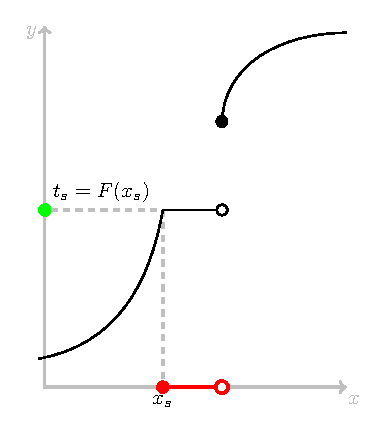
\includegraphics{distributionFunction}
        \caption{Ejemplo de funci\'on de distribuci\'on de probabilidad. En rojo se muestra la inversa $F^{-1}(t_s)$.}
	\label{f:cdf1D}
\end{figure}

Sea $S:= \{x_1, \ldots, x_n\}$ el conjunto formado por observaciones (valores medidos o muestreados) de la variable aleatoria $X$. Entonces se pueden estimar los valores de la funci\'on de distribuci\'on $F$ a partir de su funci\'on de distribuci\'on emp\'irica.

\begin{equation}
\label{e:empF} % "e"quation of the "Emp"irical Distribution function Fn.
\hat{F_n} (x) = \frac{1}{n}\sum_{k=1}^{n} \mathbbm{1} (x_k \le x)
\end{equation}

\noindent
donde $\mathbbm{1}$ es la funci\'on indicador (\autoref{e:indicatorFunc}) y $n$ es la cantidad de datos.

Esta funci\'on emp\'irica es la funci\'on no param\'etrica aproximante m\'as conocida de una funci\'on de distribuci\'on, pero tambi\'en existen otras como la de Weibull plotting position \'o est\'andar \citep[p. 10]{salvadori_extremes_2007}.
No se debe confundir con la unci\'on de densidad de Weibull, la cual es continua. En este trabajo utilizaremos la \autoref{e:empF} debido a su simplicidad y a su similitud con la c\'opula emp\'irica que se ver\'a m\'as adelante.

A partir de ahora, en lo que resta de esta subsecci\'on, supondremos que los datos observados $x_i$ est\'an ordenados en orden creciente ($x_i < x_{i+1}$) y no hay datos duplicados, es decir, que los datos son iguales a sus estad\'isticos de orden $x_{(i)}$.

El gr\'afico de la funci\'on de distribuci\'on emp\'irica (\autoref{f:empCDF}) es constante a tramos con saltos de magnitud $1/n$ cada $x_i$.
%En cada salto, los puntos rellenos representan un punto en la curva $\hat{F_n}$ mientras que los puntos vac\'ios representan un punto que \textit{no} pertenece a la funci\'on de distribuci\'on emp\'irica.
Si definimos las \textbf{pseudo-observaciones} como $u_i := \hat{F_n}(x_i)$,
%entonces los puntos rellenos tienen coordenadas $(x_i, u_i)$.
interpretada como una probabilidad en el intervalo $[0,1]$, $u_i$ es una cantidad adimensional.

\begin{figure}[H]
	\centering
	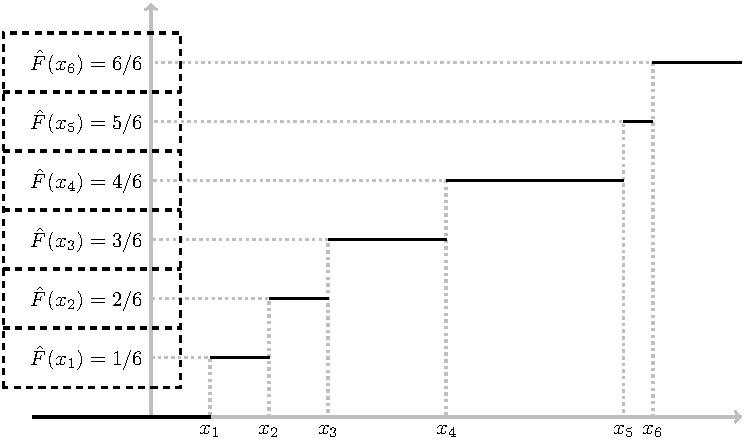
\includegraphics{empCDF}
	\caption{Funci\'on de distribuci\'on emp\'irica. Los rect\'angulos en negro con l\'ineas de guiones se muestra el correspondiente arreglo computacional para almacenar los valores de $\hat{F}_n$.}
	\label{f:empCDF}
\end{figure}

Desde el punto de vista computacional, para obtener valores de esta funci\'on emp\'irica solamente basta con almacenar los valores de $\hat{F}_n(x_i)$, para toda $i=1,\ldots, n$.

$$
\begin{array}{| c | c | c | c | c | c |}
	\hline
	\hat{F}_n(x_1) & \hat{F}_n(x_2) & \hat{F}_n(x_3) & \cdots & \hat{F}_n(x_{n-1}) & \hat{F}_n(x_n) \\ \hline
\end{array}
$$

De esta manera para saber el valor de $\hat{F}_n$ en cualquier otro valor $x$, solamente hay que compararlo contra todas las observaciones y saber cu\'al $x_i$ es el inmediato inferior.
Esto es lo que significa la \autoref{e:empF}: para obtener un valor $\hat{F}(x)$, $x$ se compara con cada observaci\'on $x_i$.
N\'otese que ya no se requieren los valores $x_i$ ya que est\'an impl\'icitos en vector de valores de $\hat{F}_n$, solamente es necesario saber cu\'al es el \'indice $i$ para poder acceder al arreglo.
Para lenguajes de programaci\'on de bajo nivel como C/C++ o Fortran, esto se pudiera implementar en un arreglo de enteros sin signo, lo que reduce el uso de memoria comparado con un arreglo de n\'umeros reales (valores flotantes).
Los \'indices de la \autoref{f:empCDF} corresponden uno-a-uno con arreglos de lenguajes de programaci\'on con offset $1$ como R o Matlab, pero no para arreglos de lenguajes programaci\'on de offset $0$ como Python o C++.
A\'un m\'as, pudiera ahorrarse guardar tal arreglo ya que el c\'alculo de $1/i$ es computacionalmente muy r\'apido.

La implementaci\'on computacional de la funci\'on de distribuci\'on emp\'irica est\'a en la funci\'on \verb|stats::ecdf| del software \verb|R|.

Como puede verse en la \autoref{f:empCDF}, la funci\'on de distribuci\'on emp\'irica no es continua, pero existen muchos modelos que s\'i lo son. Por ejemplo, se encuentran la funci\'on normal, la lognormal, ley de potencias, Weibull, exponencial, entre otras. Estos ejemplos, salvo la distribuci\'on normal, tienen asimetr\'ia positiva, y son com\'unmente utilizadas en el modelado de las longitudes de fracturas \citep{bonnet_scaling_2001,bour_connectivity_1997,gudmundsson_power-law_2011}. Aunque estas distribuciones dependen de ciertos par\'ametros (la media y la varianza en el caso de la distribuci\'on normal), tambi\'en existen funciones de distribuci\'on no param\'etricas. Otras variables que pueden ser modeladas con dichas funciones son la apertura, la porosidad y la permeabilidad.

En muchas ocasiones unos de los objetivos buscados mediante el an\'alisis y modelado de los datos es la simulaci\'on, ya que permite cuantificar la incertidumbre del fen\'omeno. Un algoritmo de simulaci\'on denominado de la transformada inversa requiere la funci\'on cuantil. \'Esta es una funci\'on asociada con una variable aleatoria $X$, la cual se define como la inversa generalizada $F^-:[0,1] \to \overline{\mathbb{R}}= [-\infty, \infty]$ de la funci\'on de distribuci\'on $F$ \citep{embrechts_note_2013}:

\begin{equation}
	F^-(y)= \inf \{x \in \mathbb{R}:F(x) \ge y\}
	\label{e:generalizedInv}
\end{equation}

\noindent
con la convenci\'on que $\inf \emptyset = \infty$. Esta inversa puede visualizarse en la \autoref{f:cdf1D}. Si $F$ es estrictamente creciente, entonces $F^- = F^{-1}$, la inversa generalizada es igual a la inversa usual.

Dicha funci\'on cuantil, puede o no existir en forma expl\'icita independientemente si la funci\'on $F$ existe en forma expl\'icita. Por ejemplo, se tiene una f\'ormula algebraica para la funci\'on de densidad de la distribuci\'on normal pero no se tiene una para calcular la funci\'on de distribuci\'on o la funci\'on cuantil, para estos casos se tiene que recurrir a m\'etodos num\'ericos. Un ejemplo parecido es el encontrado con la funci\'on de densidad de von Mises (V\'ease \autoref{ss:circularStats}).

Un ejemplo opuesto se tiene con los polinomios de Bernstein-Kantorovich \citep{munoz-perez_estimating_1987}, que representan de forma semi-expl\'icita la funci\'on cuantil, pero para obtener su correspondiente funci\'on de distribuci\'on se tiene que recurrir a m\'etodos num\'ericos \citep{quarteroni_numerical_2006,dahlquist_numerical_2008}. Esta funci\'on no param\'etrica y continua es un caso particular de una curva de B\'ezier (ver \autoref{ch:approxTheory}). La implementaci\'on computacional de esta funci\'on puede ser utilizada mediante la funci\'on \verb|lmomco::dat2bernqua| \citep{asquith_lmomco:_2017}.

Encontrar num\'ericamente la inversa de una funci\'on $F$ para un valor $y$ en su imagen, es equivalente a encontrar la ra\'iz $x$ de la funci\'on $G(x,y)= F(x) - y = 0$. Una implementaci\'on computacional para encontrar dicha ra\'iz se puede encontrar en el software R con la funci\'on \verb|stats::uniroot|. Otra funci\'on que podr\'ia ser m\'as r\'apida es utilizando una versi\'on paralelizada del m\'etodo de bisecci\'on para encontrar dicha ra\'iz \citep{miranker_survey_1971,nijmeijer_parallel_2015,stack_overflow_algorithm_2017,karniadakis_parallel_2003}. Tambi\'en se puede aprovechar el hecho de que la funci\'on $G$, debido a que es una traslaci\'on de $F$, es mon\'otona.


% \chapter{Estad\'istica de datos orientados}
\label{ch:prob}

Antes de revisar el tema principal de este cap\'itulo es conveniente revisar algunos temas de probabilidad que son comunes o equivalentes.

\section{Variables aleatorias}
\label{s:randomVar}

Una variable aleatoria es una funci\'on en donde el dominio es un espacio de posibles opciones $S$ y la imagen son los n\'umeros reales $\mathbb{R}$ \citep{casella_statistical_2002}.
El t\'ermino \textit{aleatorio} en la definici\'on hace referencia a la ley probabilidad y no significa que tenga la misma probabilidad en cualquier intervalo de su imagen. A largo de este escrito se entender\'a de esta manera.

\textit{Notaci\'on}: Las variables aleatorias se denotar\'an con letras may\'usculas, $X$ por ejemplo. Por otro lado, las realizaciones/observaciones de esta variable aleatoria (o su imagen) ser\'an denotadas con las correspondientes letras min\'usculas, $x$ para el ejemplo anterior. A diferencia del cap\'itulo anterior en que $x$ y $X$ indicaban ubicaci\'on espacial, en este cap\'itulo y el que sigue se utilizar\'a para referirnos a una variable aleatoria.
%Como ejemplo m\'as espec\'ifico tenemos el siguiente: $X$, la estatura de los mexicanos, puede tomar el valor $x=1.7$ m.

El objeto de estudio de este proyecto doctoral fueron fen\'omenos que se modelaron con variables aleatorias continuas, es decir, variables aleatorias cuya imagen pod\'ia tomar cualquier valor dentro de cierto intervalo no nulo de los reales.

Las funciones aleatorias son completamente caracterizadas por su funci\'on de distribuci\'on de probabilidad $F$, tambi\'en conocidas como funci\'on de distribuci\'on acumulativa (CDF, por sus siglas en ingl\'es):

\begin{equation}
	F_X(x) = P_X(X \le x), \qquad \forall x. 
	\label{e:cdf1D}
\end{equation}

\noindent
donde $P$ denota la probabilidad de que la variable aleatoria $X$ sea menor o igual que el valor $x$.
%Por ejemplo, la probabilidad de que la estatura, $X$, sea menor que $x = 1.5$ m.

Para caracterizar completamente una variable aleatoria continua $X$, alternativamente a la funci\'on de distribuci\'on $F$, se tiene la funci\'on de densidad de probabilidad $f$:

\begin{equation}
	F_X(x) = \int_{-\infty}^x f_X(t)dt \qquad \forall x.
\end{equation}

Si $f_X(x)$ es continua, entonces, por el teorema fundamental del c\'alculo:

\begin{equation}
	\frac{d}{dx}F_X(x) = f_X(x)
\end{equation}

El histograma es un estimador de la funci\'on de densidad $f_X$.

Para mostrar las caracter\'isticas de una CDF usemos la diferencia hacia adelante de primer orden:

\begin{equation}
\label{e:ForwDiff} % "Forw"ard "Diff"erence
\Delta F :=F(x+d)-F(x)
\end{equation}

Una funci\'on de distribuci\'on $F$ satisface las siguientes condiciones:

\begin{itemize}
	\item $F(x)$ es una funci\'on no-decreciente de $x$. Es decir, $\Delta F \ge 0$.
	\item $F(x)$ continua por la derecha. Es decir, para cada n\'umero $x_0$, $\lim_{x \to x_0^+}F(x) = F(x_0)$.
	\item $\lim_{x \to -\infty}F(x) = 0$, y  $\lim_{x \to +\infty}F(x) = 1$.
\end{itemize}

N\'otese que no hay significado probabil\'istico en estas definiciones, dicha interpretaci\'on se obtiene a partir de la definici\'on en la \autoref{e:cdf1D}. Gr\'aficamente, todas estas caracter\'isticas se pueden observar en la \autoref{f:cdf1D}.

\begin{figure}
	\centering
	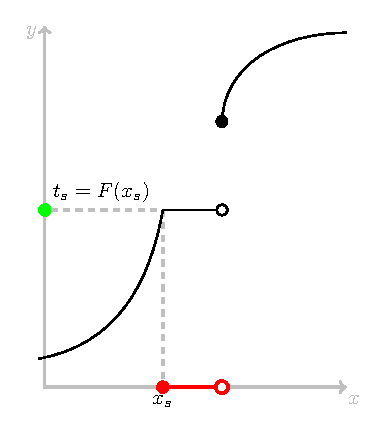
\includegraphics{distributionFunction}
        \caption{Ejemplo de funci\'on de distribuci\'on de probabilidad. En rojo se muestra la inversa $F^{-1}(t_s)$.}
	\label{f:cdf1D}
\end{figure}

Sea $S:= \{x_1, \ldots, x_n\}$ el conjunto formado por observaciones (valores medidos o muestreados) de la variable aleatoria $X$. Entonces se pueden estimar los valores de la funci\'on de distribuci\'on $F$ a partir de su funci\'on de distribuci\'on emp\'irica.

\begin{equation}
\label{e:empF} % "e"quation of the "Emp"irical Distribution function Fn.
\hat{F_n} (x) = \frac{1}{n}\sum_{k=1}^{n} \mathbbm{1} (x_k \le x)
\end{equation}

\noindent
donde $\mathbbm{1}$ es la funci\'on indicador (\autoref{e:indicatorFunc}) y $n$ es la cantidad de datos.

Esta funci\'on emp\'irica es la funci\'on no param\'etrica aproximante m\'as conocida de una funci\'on de distribuci\'on, pero tambi\'en existen otras como la de Weibull plotting position \'o est\'andar \citep[p. 10]{salvadori_extremes_2007}.
No se debe confundir con la unci\'on de densidad de Weibull, la cual es continua. En este trabajo utilizaremos la \autoref{e:empF} debido a su simplicidad y a su similitud con la c\'opula emp\'irica que se ver\'a m\'as adelante.

A partir de ahora, en lo que resta de esta subsecci\'on, supondremos que los datos observados $x_i$ est\'an ordenados en orden creciente ($x_i < x_{i+1}$) y no hay datos duplicados, es decir, que los datos son iguales a sus estad\'isticos de orden $x_{(i)}$.

El gr\'afico de la funci\'on de distribuci\'on emp\'irica (\autoref{f:empCDF}) es constante a tramos con saltos de magnitud $1/n$ cada $x_i$.
%En cada salto, los puntos rellenos representan un punto en la curva $\hat{F_n}$ mientras que los puntos vac\'ios representan un punto que \textit{no} pertenece a la funci\'on de distribuci\'on emp\'irica.
Si definimos las \textbf{pseudo-observaciones} como $u_i := \hat{F_n}(x_i)$,
%entonces los puntos rellenos tienen coordenadas $(x_i, u_i)$.
interpretada como una probabilidad en el intervalo $[0,1]$, $u_i$ es una cantidad adimensional.

\begin{figure}[H]
	\centering
	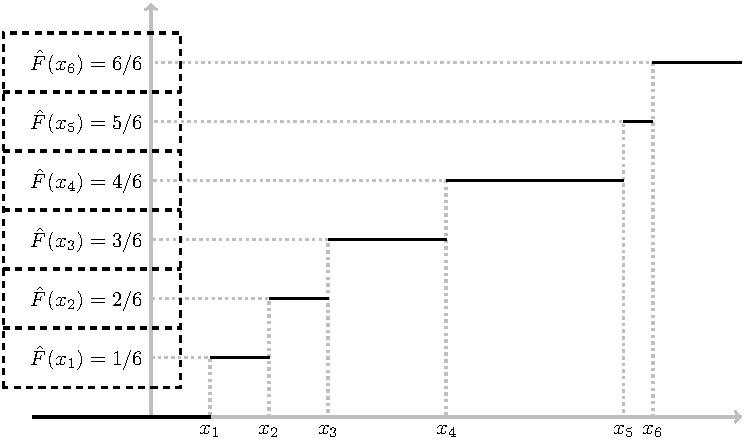
\includegraphics{empCDF}
	\caption{Funci\'on de distribuci\'on emp\'irica. Los rect\'angulos en negro con l\'ineas de guiones se muestra el correspondiente arreglo computacional para almacenar los valores de $\hat{F}_n$.}
	\label{f:empCDF}
\end{figure}

Desde el punto de vista computacional, para obtener valores de esta funci\'on emp\'irica solamente basta con almacenar los valores de $\hat{F}_n(x_i)$, para toda $i=1,\ldots, n$.

$$
\begin{array}{| c | c | c | c | c | c |}
	\hline
	\hat{F}_n(x_1) & \hat{F}_n(x_2) & \hat{F}_n(x_3) & \cdots & \hat{F}_n(x_{n-1}) & \hat{F}_n(x_n) \\ \hline
\end{array}
$$

De esta manera para saber el valor de $\hat{F}_n$ en cualquier otro valor $x$, solamente hay que compararlo contra todas las observaciones y saber cu\'al $x_i$ es el inmediato inferior.
Esto es lo que significa la \autoref{e:empF}: para obtener un valor $\hat{F}(x)$, $x$ se compara con cada observaci\'on $x_i$.
N\'otese que ya no se requieren los valores $x_i$ ya que est\'an impl\'icitos en vector de valores de $\hat{F}_n$, solamente es necesario saber cu\'al es el \'indice $i$ para poder acceder al arreglo.
Para lenguajes de programaci\'on de bajo nivel como C/C++ o Fortran, esto se pudiera implementar en un arreglo de enteros sin signo, lo que reduce el uso de memoria comparado con un arreglo de n\'umeros reales (valores flotantes).
Los \'indices de la \autoref{f:empCDF} corresponden uno-a-uno con arreglos de lenguajes de programaci\'on con offset $1$ como R o Matlab, pero no para arreglos de lenguajes programaci\'on de offset $0$ como Python o C++.
A\'un m\'as, pudiera ahorrarse guardar tal arreglo ya que el c\'alculo de $1/i$ es computacionalmente muy r\'apido.

La implementaci\'on computacional de la funci\'on de distribuci\'on emp\'irica est\'a en la funci\'on \verb|stats::ecdf| del software \verb|R|.

Como puede verse en la \autoref{f:empCDF}, la funci\'on de distribuci\'on emp\'irica no es continua, pero existen muchos modelos que s\'i lo son. Por ejemplo, se encuentran la funci\'on normal, la lognormal, ley de potencias, Weibull, exponencial, entre otras. Estos ejemplos, salvo la distribuci\'on normal, tienen asimetr\'ia positiva, y son com\'unmente utilizadas en el modelado de las longitudes de fracturas \citep{bonnet_scaling_2001,bour_connectivity_1997,gudmundsson_power-law_2011}. Aunque estas distribuciones dependen de ciertos par\'ametros (la media y la varianza en el caso de la distribuci\'on normal), tambi\'en existen funciones de distribuci\'on no param\'etricas. Otras variables que pueden ser modeladas con dichas funciones son la apertura, la porosidad y la permeabilidad.

En muchas ocasiones unos de los objetivos buscados mediante el an\'alisis y modelado de los datos es la simulaci\'on, ya que permite cuantificar la incertidumbre del fen\'omeno. Un algoritmo de simulaci\'on denominado de la transformada inversa requiere la funci\'on cuantil. \'Esta es una funci\'on asociada con una variable aleatoria $X$, la cual se define como la inversa generalizada $F^-:[0,1] \to \overline{\mathbb{R}}= [-\infty, \infty]$ de la funci\'on de distribuci\'on $F$ \citep{embrechts_note_2013}:

\begin{equation}
	F^-(y)= \inf \{x \in \mathbb{R}:F(x) \ge y\}
	\label{e:generalizedInv}
\end{equation}

\noindent
con la convenci\'on que $\inf \emptyset = \infty$. Esta inversa puede visualizarse en la \autoref{f:cdf1D}. Si $F$ es estrictamente creciente, entonces $F^- = F^{-1}$, la inversa generalizada es igual a la inversa usual.

Dicha funci\'on cuantil, puede o no existir en forma expl\'icita independientemente si la funci\'on $F$ existe en forma expl\'icita. Por ejemplo, se tiene una f\'ormula algebraica para la funci\'on de densidad de la distribuci\'on normal pero no se tiene una para calcular la funci\'on de distribuci\'on o la funci\'on cuantil, para estos casos se tiene que recurrir a m\'etodos num\'ericos. Un ejemplo parecido es el encontrado con la funci\'on de densidad de von Mises (V\'ease \autoref{ss:circularStats}).

Un ejemplo opuesto se tiene con los polinomios de Bernstein-Kantorovich \citep{munoz-perez_estimating_1987}, que representan de forma semi-expl\'icita la funci\'on cuantil, pero para obtener su correspondiente funci\'on de distribuci\'on se tiene que recurrir a m\'etodos num\'ericos \citep{quarteroni_numerical_2006,dahlquist_numerical_2008}. Esta funci\'on no param\'etrica y continua es un caso particular de una curva de B\'ezier (ver \autoref{ch:approxTheory}). La implementaci\'on computacional de esta funci\'on puede ser utilizada mediante la funci\'on \verb|lmomco::dat2bernqua| \citep{asquith_lmomco:_2017}.

Encontrar num\'ericamente la inversa de una funci\'on $F$ para un valor $y$ en su imagen, es equivalente a encontrar la ra\'iz $x$ de la funci\'on $G(x,y)= F(x) - y = 0$. Una implementaci\'on computacional para encontrar dicha ra\'iz se puede encontrar en el software R con la funci\'on \verb|stats::uniroot|. Otra funci\'on que podr\'ia ser m\'as r\'apida es utilizando una versi\'on paralelizada del m\'etodo de bisecci\'on para encontrar dicha ra\'iz \citep{miranker_survey_1971,nijmeijer_parallel_2015,stack_overflow_algorithm_2017,karniadakis_parallel_2003}. Tambi\'en se puede aprovechar el hecho de que la funci\'on $G$, debido a que es una traslaci\'on de $F$, es mon\'otona.


% \chapter{Estad\'istica de datos orientados}
\label{ch:prob}

Antes de revisar el tema principal de este cap\'itulo es conveniente revisar algunos temas de probabilidad que son comunes o equivalentes.

\section{Variables aleatorias}
\label{s:randomVar}

Una variable aleatoria es una funci\'on en donde el dominio es un espacio de posibles opciones $S$ y la imagen son los n\'umeros reales $\mathbb{R}$ \citep{casella_statistical_2002}.
El t\'ermino \textit{aleatorio} en la definici\'on hace referencia a la ley probabilidad y no significa que tenga la misma probabilidad en cualquier intervalo de su imagen. A largo de este escrito se entender\'a de esta manera.

\textit{Notaci\'on}: Las variables aleatorias se denotar\'an con letras may\'usculas, $X$ por ejemplo. Por otro lado, las realizaciones/observaciones de esta variable aleatoria (o su imagen) ser\'an denotadas con las correspondientes letras min\'usculas, $x$ para el ejemplo anterior. A diferencia del cap\'itulo anterior en que $x$ y $X$ indicaban ubicaci\'on espacial, en este cap\'itulo y el que sigue se utilizar\'a para referirnos a una variable aleatoria.
%Como ejemplo m\'as espec\'ifico tenemos el siguiente: $X$, la estatura de los mexicanos, puede tomar el valor $x=1.7$ m.

El objeto de estudio de este proyecto doctoral fueron fen\'omenos que se modelaron con variables aleatorias continuas, es decir, variables aleatorias cuya imagen pod\'ia tomar cualquier valor dentro de cierto intervalo no nulo de los reales.

Las funciones aleatorias son completamente caracterizadas por su funci\'on de distribuci\'on de probabilidad $F$, tambi\'en conocidas como funci\'on de distribuci\'on acumulativa (CDF, por sus siglas en ingl\'es):

\begin{equation}
	F_X(x) = P_X(X \le x), \qquad \forall x. 
	\label{e:cdf1D}
\end{equation}

\noindent
donde $P$ denota la probabilidad de que la variable aleatoria $X$ sea menor o igual que el valor $x$.
%Por ejemplo, la probabilidad de que la estatura, $X$, sea menor que $x = 1.5$ m.

Para caracterizar completamente una variable aleatoria continua $X$, alternativamente a la funci\'on de distribuci\'on $F$, se tiene la funci\'on de densidad de probabilidad $f$:

\begin{equation}
	F_X(x) = \int_{-\infty}^x f_X(t)dt \qquad \forall x.
\end{equation}

Si $f_X(x)$ es continua, entonces, por el teorema fundamental del c\'alculo:

\begin{equation}
	\frac{d}{dx}F_X(x) = f_X(x)
\end{equation}

El histograma es un estimador de la funci\'on de densidad $f_X$.

Para mostrar las caracter\'isticas de una CDF usemos la diferencia hacia adelante de primer orden:

\begin{equation}
\label{e:ForwDiff} % "Forw"ard "Diff"erence
\Delta F :=F(x+d)-F(x)
\end{equation}

Una funci\'on de distribuci\'on $F$ satisface las siguientes condiciones:

\begin{itemize}
	\item $F(x)$ es una funci\'on no-decreciente de $x$. Es decir, $\Delta F \ge 0$.
	\item $F(x)$ continua por la derecha. Es decir, para cada n\'umero $x_0$, $\lim_{x \to x_0^+}F(x) = F(x_0)$.
	\item $\lim_{x \to -\infty}F(x) = 0$, y  $\lim_{x \to +\infty}F(x) = 1$.
\end{itemize}

N\'otese que no hay significado probabil\'istico en estas definiciones, dicha interpretaci\'on se obtiene a partir de la definici\'on en la \autoref{e:cdf1D}. Gr\'aficamente, todas estas caracter\'isticas se pueden observar en la \autoref{f:cdf1D}.

\begin{figure}
	\centering
	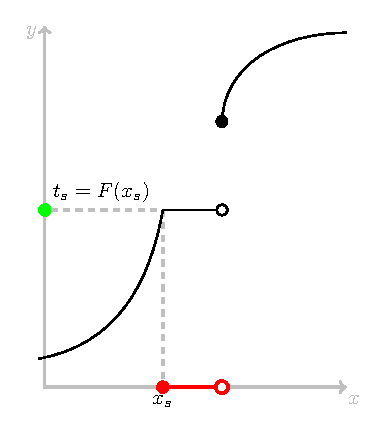
\includegraphics{distributionFunction}
        \caption{Ejemplo de funci\'on de distribuci\'on de probabilidad. En rojo se muestra la inversa $F^{-1}(t_s)$.}
	\label{f:cdf1D}
\end{figure}

Sea $S:= \{x_1, \ldots, x_n\}$ el conjunto formado por observaciones (valores medidos o muestreados) de la variable aleatoria $X$. Entonces se pueden estimar los valores de la funci\'on de distribuci\'on $F$ a partir de su funci\'on de distribuci\'on emp\'irica.

\begin{equation}
\label{e:empF} % "e"quation of the "Emp"irical Distribution function Fn.
\hat{F_n} (x) = \frac{1}{n}\sum_{k=1}^{n} \mathbbm{1} (x_k \le x)
\end{equation}

\noindent
donde $\mathbbm{1}$ es la funci\'on indicador (\autoref{e:indicatorFunc}) y $n$ es la cantidad de datos.

Esta funci\'on emp\'irica es la funci\'on no param\'etrica aproximante m\'as conocida de una funci\'on de distribuci\'on, pero tambi\'en existen otras como la de Weibull plotting position \'o est\'andar \citep[p. 10]{salvadori_extremes_2007}.
No se debe confundir con la unci\'on de densidad de Weibull, la cual es continua. En este trabajo utilizaremos la \autoref{e:empF} debido a su simplicidad y a su similitud con la c\'opula emp\'irica que se ver\'a m\'as adelante.

A partir de ahora, en lo que resta de esta subsecci\'on, supondremos que los datos observados $x_i$ est\'an ordenados en orden creciente ($x_i < x_{i+1}$) y no hay datos duplicados, es decir, que los datos son iguales a sus estad\'isticos de orden $x_{(i)}$.

El gr\'afico de la funci\'on de distribuci\'on emp\'irica (\autoref{f:empCDF}) es constante a tramos con saltos de magnitud $1/n$ cada $x_i$.
%En cada salto, los puntos rellenos representan un punto en la curva $\hat{F_n}$ mientras que los puntos vac\'ios representan un punto que \textit{no} pertenece a la funci\'on de distribuci\'on emp\'irica.
Si definimos las \textbf{pseudo-observaciones} como $u_i := \hat{F_n}(x_i)$,
%entonces los puntos rellenos tienen coordenadas $(x_i, u_i)$.
interpretada como una probabilidad en el intervalo $[0,1]$, $u_i$ es una cantidad adimensional.

\begin{figure}[H]
	\centering
	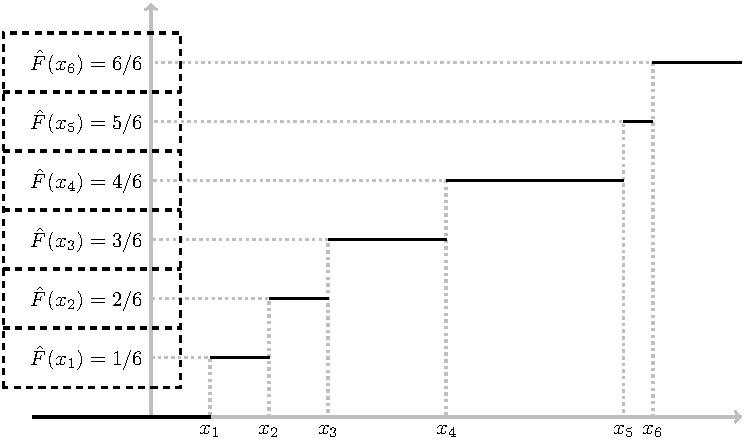
\includegraphics{empCDF}
	\caption{Funci\'on de distribuci\'on emp\'irica. Los rect\'angulos en negro con l\'ineas de guiones se muestra el correspondiente arreglo computacional para almacenar los valores de $\hat{F}_n$.}
	\label{f:empCDF}
\end{figure}

Desde el punto de vista computacional, para obtener valores de esta funci\'on emp\'irica solamente basta con almacenar los valores de $\hat{F}_n(x_i)$, para toda $i=1,\ldots, n$.

$$
\begin{array}{| c | c | c | c | c | c |}
	\hline
	\hat{F}_n(x_1) & \hat{F}_n(x_2) & \hat{F}_n(x_3) & \cdots & \hat{F}_n(x_{n-1}) & \hat{F}_n(x_n) \\ \hline
\end{array}
$$

De esta manera para saber el valor de $\hat{F}_n$ en cualquier otro valor $x$, solamente hay que compararlo contra todas las observaciones y saber cu\'al $x_i$ es el inmediato inferior.
Esto es lo que significa la \autoref{e:empF}: para obtener un valor $\hat{F}(x)$, $x$ se compara con cada observaci\'on $x_i$.
N\'otese que ya no se requieren los valores $x_i$ ya que est\'an impl\'icitos en vector de valores de $\hat{F}_n$, solamente es necesario saber cu\'al es el \'indice $i$ para poder acceder al arreglo.
Para lenguajes de programaci\'on de bajo nivel como C/C++ o Fortran, esto se pudiera implementar en un arreglo de enteros sin signo, lo que reduce el uso de memoria comparado con un arreglo de n\'umeros reales (valores flotantes).
Los \'indices de la \autoref{f:empCDF} corresponden uno-a-uno con arreglos de lenguajes de programaci\'on con offset $1$ como R o Matlab, pero no para arreglos de lenguajes programaci\'on de offset $0$ como Python o C++.
A\'un m\'as, pudiera ahorrarse guardar tal arreglo ya que el c\'alculo de $1/i$ es computacionalmente muy r\'apido.

La implementaci\'on computacional de la funci\'on de distribuci\'on emp\'irica est\'a en la funci\'on \verb|stats::ecdf| del software \verb|R|.

Como puede verse en la \autoref{f:empCDF}, la funci\'on de distribuci\'on emp\'irica no es continua, pero existen muchos modelos que s\'i lo son. Por ejemplo, se encuentran la funci\'on normal, la lognormal, ley de potencias, Weibull, exponencial, entre otras. Estos ejemplos, salvo la distribuci\'on normal, tienen asimetr\'ia positiva, y son com\'unmente utilizadas en el modelado de las longitudes de fracturas \citep{bonnet_scaling_2001,bour_connectivity_1997,gudmundsson_power-law_2011}. Aunque estas distribuciones dependen de ciertos par\'ametros (la media y la varianza en el caso de la distribuci\'on normal), tambi\'en existen funciones de distribuci\'on no param\'etricas. Otras variables que pueden ser modeladas con dichas funciones son la apertura, la porosidad y la permeabilidad.

En muchas ocasiones unos de los objetivos buscados mediante el an\'alisis y modelado de los datos es la simulaci\'on, ya que permite cuantificar la incertidumbre del fen\'omeno. Un algoritmo de simulaci\'on denominado de la transformada inversa requiere la funci\'on cuantil. \'Esta es una funci\'on asociada con una variable aleatoria $X$, la cual se define como la inversa generalizada $F^-:[0,1] \to \overline{\mathbb{R}}= [-\infty, \infty]$ de la funci\'on de distribuci\'on $F$ \citep{embrechts_note_2013}:

\begin{equation}
	F^-(y)= \inf \{x \in \mathbb{R}:F(x) \ge y\}
	\label{e:generalizedInv}
\end{equation}

\noindent
con la convenci\'on que $\inf \emptyset = \infty$. Esta inversa puede visualizarse en la \autoref{f:cdf1D}. Si $F$ es estrictamente creciente, entonces $F^- = F^{-1}$, la inversa generalizada es igual a la inversa usual.

Dicha funci\'on cuantil, puede o no existir en forma expl\'icita independientemente si la funci\'on $F$ existe en forma expl\'icita. Por ejemplo, se tiene una f\'ormula algebraica para la funci\'on de densidad de la distribuci\'on normal pero no se tiene una para calcular la funci\'on de distribuci\'on o la funci\'on cuantil, para estos casos se tiene que recurrir a m\'etodos num\'ericos. Un ejemplo parecido es el encontrado con la funci\'on de densidad de von Mises (V\'ease \autoref{ss:circularStats}).

Un ejemplo opuesto se tiene con los polinomios de Bernstein-Kantorovich \citep{munoz-perez_estimating_1987}, que representan de forma semi-expl\'icita la funci\'on cuantil, pero para obtener su correspondiente funci\'on de distribuci\'on se tiene que recurrir a m\'etodos num\'ericos \citep{quarteroni_numerical_2006,dahlquist_numerical_2008}. Esta funci\'on no param\'etrica y continua es un caso particular de una curva de B\'ezier (ver \autoref{ch:approxTheory}). La implementaci\'on computacional de esta funci\'on puede ser utilizada mediante la funci\'on \verb|lmomco::dat2bernqua| \citep{asquith_lmomco:_2017}.

Encontrar num\'ericamente la inversa de una funci\'on $F$ para un valor $y$ en su imagen, es equivalente a encontrar la ra\'iz $x$ de la funci\'on $G(x,y)= F(x) - y = 0$. Una implementaci\'on computacional para encontrar dicha ra\'iz se puede encontrar en el software R con la funci\'on \verb|stats::uniroot|. Otra funci\'on que podr\'ia ser m\'as r\'apida es utilizando una versi\'on paralelizada del m\'etodo de bisecci\'on para encontrar dicha ra\'iz \citep{miranker_survey_1971,nijmeijer_parallel_2015,stack_overflow_algorithm_2017,karniadakis_parallel_2003}. Tambi\'en se puede aprovechar el hecho de que la funci\'on $G$, debido a que es una traslaci\'on de $F$, es mon\'otona.


% \include{TeX/directionalStats}

\section{Variables orientadas}
\label{ss:circularStats}

Los \emph{datos direccionales} (tambi\'en conocidos como \emph{datos orientados}) surgen de varias maneras. En particular, cuando se trata de una dimensi\'on (una sola variable aleatoria) se les llama \emph{datos circulares} y esta variable se encuentra definida sobre el c\'irculo unitario, \(\mathbb{S}^{1} = [0, 2 \pi) \). N\'otese que \'esta es una variable aleatoria con periodo \(2\pi\). Algunos ejemplos de variables aleatorias peri\'odicas son la direcci\'on de una br\'ujula (como direcci\'on del viento, direcci\'on del vuelo, direcci\'on de rumbo, etc.), la posici\'on de las manecillas del reloj, la temperatura diurna, o la anual, etc.

En la caracterizaci\'on de fracturas o fallas geol\'ogicas, se cuenta con datos cuya caracter\'istica es tener dos componentes de este estilo. Estas componentes son el \emph{echado} y \emph{azimut}; ambas asociadas a un solo dato y ambas medidas en \'angulos. Estas dos componentes generan un vector (o dato) en 3D, por lo que la herramienta que se deber\'ia considerar para el an\'alisis estad\'istico son los \emph{datos esf\'ericos} \cite{fisher_statistical_1993,jammalamadaka_topics_2001}.

En el caso univariado, la estad\'istica de datos orientados surge de manera natural si se intenta calcular la media y la desviaci\'on est\'andar del conjunto de datos que se muestra en la Figura 1. N\'otese que, si se calcula el promedio usual, el valor estimado para la media ser\'ia de 180$^\circ$~=~(10+350)/2, la cual es una direcci\'on diametralmente opuesta a la sugerida por los datos (0$^\circ$~= Este geogr\'afico). Tambi\'en n\'otese que si se procede con este camino la varianza correspondiente tambi\'en discrepa mucho de lo que se observa en el \emph{histograma circular} de la izquierda de la figura.


\begin{figure}[H]
	\centering 
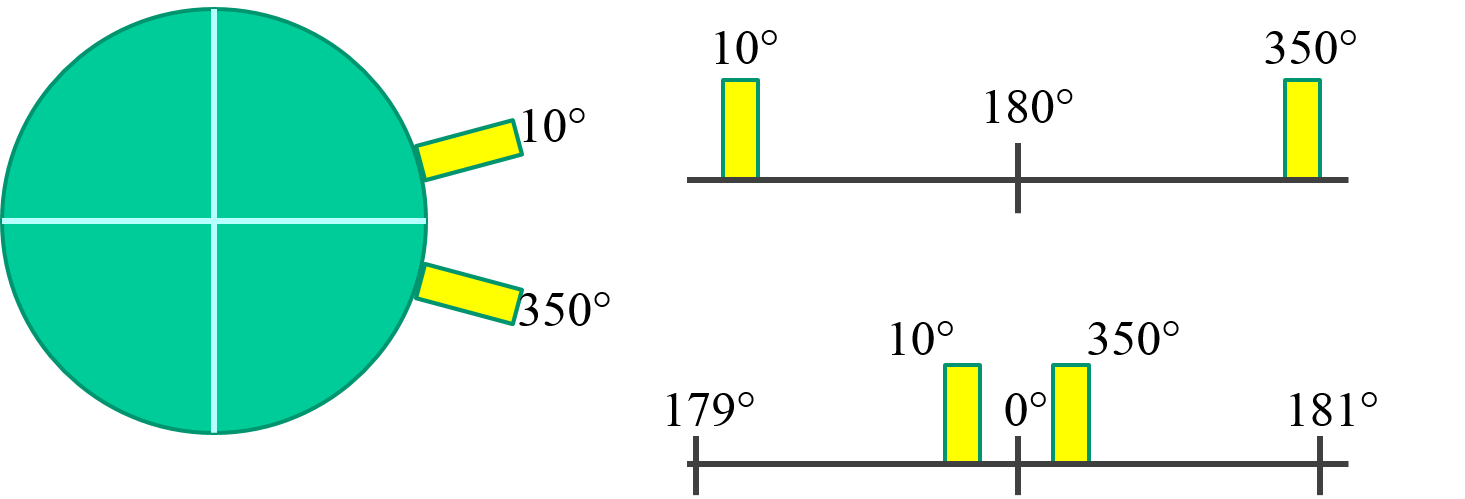
\includegraphics[width=4.30250in,height=1.46419in]{directional_histogram}
	\caption{Motivaci\'on de la estad\'istica de datos orientados. \textquestiondown Cu\'al es la media? \textquestiondown Y la desviaci\'on est\'andar?}
	\label{f:directionalHist}
\end{figure}

La soluci\'on a este problema lo proporciona la estad\'istica de datos orientados al hacer uso del c\'alculo vectorial. Con este enfoque los estad\'igrafos b\'asicos para datos circulares se definen de la siguiente manera \citep[ch. 2]{mardia_directional_2000} y est\'an implementados en el paquete \verb|circular| del software estad\'istico \verb|R|:

Supongamos que se tienen \(n\) datos, si cada orientaci\'on \(\theta_{i}\) se puede hacer corresponder con un vector unitario \(\mathbf{x}_{\mathbf{i}} = ( \cos\theta_{i},\sin\theta_{i} )\); entonces la direcci\'on media \(\overline{\theta}\) es la direcci\'on del vector resultante \(\mathbf{x}_{\mathbf{1}} + \ldots + \mathbf{x}_{\mathbf{n}}\). Las coordenadas cartesianas del centro de masa son \(( \overline{C},\ \overline{S} )\), donde

\begin{equation}
\overline{C} = \frac{1}{n}\sum_{j = 1}^{n}{\cos\theta_{j}},
\quad
\overline{S} = \frac{1}{n}\sum_{j = 1}^{n}{\sin\theta_{j}}
\end{equation}

Por lo tanto \(\overline{\theta}\) es la soluci\'on a las ecuaciones

\begin{equation}
\overline{C} = \overline{R}\cos\overline{\theta},
\quad
\overline{S} = \overline{R}\operatorname{sen}\overline{\theta}\end{equation}

Donde la longitud resultante media \(\overline{R}\) est\'a dada por

\begin{equation}
\overline{R} = \sqrt{{\overline{C}}^{2} + {\overline{S}}^{2}} \end{equation}

Observe que \(0 \leq \overline{R} \leq 1\). Si las direcciones \(\theta_{1},\ldots,\theta_{n}\) son muy cercanas entre s\'i, entonces \(\overline{R}\) ser\'a cercano a 1, pero si est\'a muy dispersas entonces \(\overline{R}\) ser\'a cercano a 0. Por lo tanto \(\overline{R}\) es una medida de \emph{concentraci\'on} de los datos. N\'otese que en la \emph{estad\'istica convencional} (o de \emph{datos no orientados}), la varianza nos proporciona una medida de \emph{dispersi\'on}, opuesto a la interpretaci\'on de \(\overline{R}.\) An\'alogo a la varianza convencional y otros estad\'igrafos pueden encontrarse en el cap\'itulo 2 de \cite{mardia_directional_2000}. Para datos esf\'ericos o datos direccionales en \(\mathbb{R}^{p}\), consulte el cap\'itulo 9 del mismo libro o el libro de \cite{fisher_statistical_1993}.

Supongamos que se ha especificado una direcci\'on (origen) y orientaci\'on (sentido de giro) inicial. Dos ejemplos de tal especificaci\'on son: 1) un plano cartesiano matem\'atico (\(X^{+} = 0,\ Y^{+} = 90\)), y 2) uno geogr\'afico (N=0$^\circ$, E=90$^\circ$). Entonces la funci\'on de distribuci\'on \(F\) para un \'angulo aleatorio \(\theta\) se define como la funci\'on en
\(\mathbb{R}\) dada por

\[F( x ) = \mathrm{\Pr}( 0 < \theta \leq x )\]

\[0 \leq x \leq 2\pi\]

y

 \(F( x + 2\pi ) - F( x ) = 1\)
\(- \infty < x < \infty\) 

La ecuaci\'on significa que cualquier arco de longitud \(2\pi\) tiene probabilidad 1 (ya que tal arco es la totalidad de la circunferencia del c\'irculo).

A diferencia de distribuciones en los reales, \(\mathbb{R}\),

\[{F( x )} = \infty, \qquad
{F( x )} = - \infty\]

Por definici\'on,

\[F( 0 ) = 0, \qquad
F( 2\pi ) = 1\]

Para una variable circular, una funci\'on \(f\) es la densidad de probabilidad de una funci\'on de distribuci\'on totalmente (absolutely) continua si y s\'olo si

\begin{itemize}
\item
  \(f( \theta ) \geq 0\) casi por doquier en
  \(( - \infty,\infty )\),
\item
  \(f( \theta + 2k\pi ) = f( \theta )\) casi por
  doquier en \(( - \infty,\infty )\) con \(k\mathbb{\in Z}\)
  (i.e., \(f\) es peri\'odica),
\item
  \(\int_{0}^{2\pi}{f( \theta )\text{d}} = 1\).
\end{itemize}

Las funciones de densidad uni y bidimensional de probabilidad param\'etricas para datos orientados m\'as comunes son:

\begin{table}[H]
	\centering
	\label{tab:directionalModels}
	\begin{tabular}{|r|l|}
\hline
von Mises &
$f( \theta;\mu,\kappa ) = \frac{1}{2\pi I_{0}( \kappa )}e^{\kappa\cos( \theta - \mu )}$ \\
\hline
Fisher &
$f( \theta,\ \phi;\alpha,\beta,\ \kappa ) = \frac{1}{4\pi\sinh( \kappa )}\exp
[ \kappa\lbrack \operatorname{sen}\theta\operatorname{sen}\alpha\cos( \phi - \beta ) + \cos\theta\cos\alpha \rbrack ] \sin\theta$
\\ \hline
	\end{tabular}
	\caption{Funciones de densidad de probabilidad para datos orientados. $0 \le \theta < 2\pi, \quad 0 \le \phi < \pi/2,\quad 0 \le \kappa < \infty$. Ver ec. 3.5.17 de \cite{mardia_directional_2000}, ec. 2.2.6 en la secci\'on 2.2.4 de \cite{jammalamadaka_topics_2001} y ec. 4.22 de \cite{fisher_statistical_1993}.}
\end{table}

La funci\'on de densidad de von-Mises es el an\'alogo a la funci\'on de densidad de probabilidad normal ya que tambi\'en consta de dos par\'ametros, es unimodal y sim\'etrica.


\section{Variables orientadas}
\label{ss:circularStats}

Los \emph{datos direccionales} (tambi\'en conocidos como \emph{datos orientados}) surgen de varias maneras. En particular, cuando se trata de una dimensi\'on (una sola variable aleatoria) se les llama \emph{datos circulares} y esta variable se encuentra definida sobre el c\'irculo unitario, \(\mathbb{S}^{1} = [0, 2 \pi) \). N\'otese que \'esta es una variable aleatoria con periodo \(2\pi\). Algunos ejemplos de variables aleatorias peri\'odicas son la direcci\'on de una br\'ujula (como direcci\'on del viento, direcci\'on del vuelo, direcci\'on de rumbo, etc.), la posici\'on de las manecillas del reloj, la temperatura diurna, o la anual, etc.

En la caracterizaci\'on de fracturas o fallas geol\'ogicas, se cuenta con datos cuya caracter\'istica es tener dos componentes de este estilo. Estas componentes son el \emph{echado} y \emph{azimut}; ambas asociadas a un solo dato y ambas medidas en \'angulos. Estas dos componentes generan un vector (o dato) en 3D, por lo que la herramienta que se deber\'ia considerar para el an\'alisis estad\'istico son los \emph{datos esf\'ericos} \cite{fisher_statistical_1993,jammalamadaka_topics_2001}.

En el caso univariado, la estad\'istica de datos orientados surge de manera natural si se intenta calcular la media y la desviaci\'on est\'andar del conjunto de datos que se muestra en la Figura 1. N\'otese que, si se calcula el promedio usual, el valor estimado para la media ser\'ia de 180$^\circ$~=~(10+350)/2, la cual es una direcci\'on diametralmente opuesta a la sugerida por los datos (0$^\circ$~= Este geogr\'afico). Tambi\'en n\'otese que si se procede con este camino la varianza correspondiente tambi\'en discrepa mucho de lo que se observa en el \emph{histograma circular} de la izquierda de la figura.


\begin{figure}[H]
	\centering 
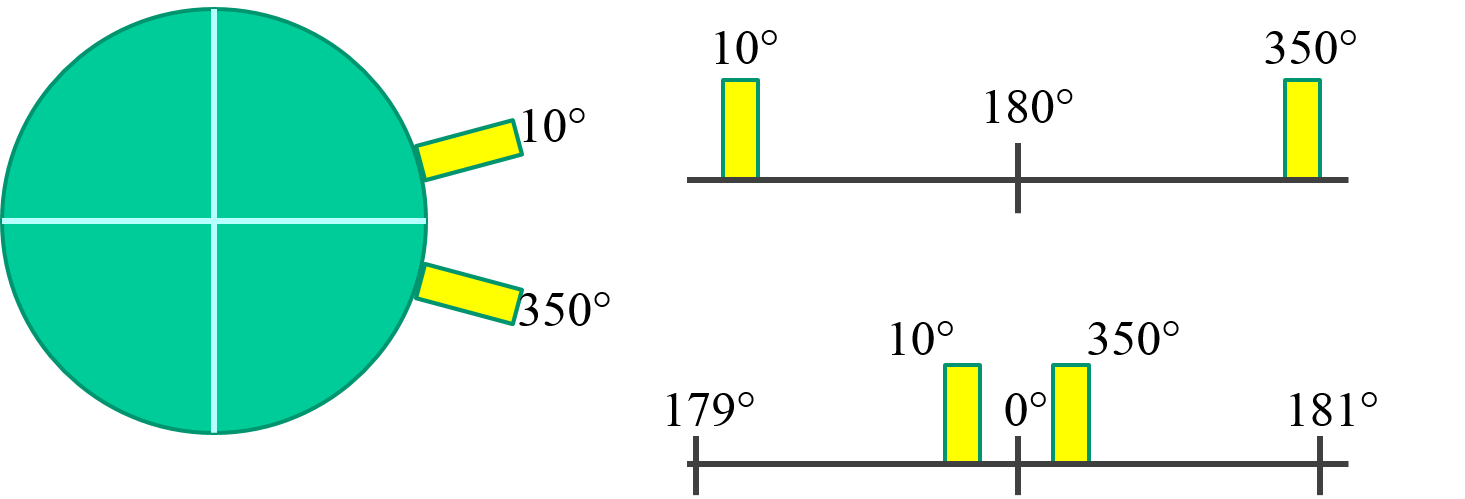
\includegraphics[width=4.30250in,height=1.46419in]{directional_histogram}
	\caption{Motivaci\'on de la estad\'istica de datos orientados. \textquestiondown Cu\'al es la media? \textquestiondown Y la desviaci\'on est\'andar?}
	\label{f:directionalHist}
\end{figure}

La soluci\'on a este problema lo proporciona la estad\'istica de datos orientados al hacer uso del c\'alculo vectorial. Con este enfoque los estad\'igrafos b\'asicos para datos circulares se definen de la siguiente manera \citep[ch. 2]{mardia_directional_2000} y est\'an implementados en el paquete \verb|circular| del software estad\'istico \verb|R|:

Supongamos que se tienen \(n\) datos, si cada orientaci\'on \(\theta_{i}\) se puede hacer corresponder con un vector unitario \(\mathbf{x}_{\mathbf{i}} = ( \cos\theta_{i},\sin\theta_{i} )\); entonces la direcci\'on media \(\overline{\theta}\) es la direcci\'on del vector resultante \(\mathbf{x}_{\mathbf{1}} + \ldots + \mathbf{x}_{\mathbf{n}}\). Las coordenadas cartesianas del centro de masa son \(( \overline{C},\ \overline{S} )\), donde

\begin{equation}
\overline{C} = \frac{1}{n}\sum_{j = 1}^{n}{\cos\theta_{j}},
\quad
\overline{S} = \frac{1}{n}\sum_{j = 1}^{n}{\sin\theta_{j}}
\end{equation}

Por lo tanto \(\overline{\theta}\) es la soluci\'on a las ecuaciones

\begin{equation}
\overline{C} = \overline{R}\cos\overline{\theta},
\quad
\overline{S} = \overline{R}\operatorname{sen}\overline{\theta}\end{equation}

Donde la longitud resultante media \(\overline{R}\) est\'a dada por

\begin{equation}
\overline{R} = \sqrt{{\overline{C}}^{2} + {\overline{S}}^{2}} \end{equation}

Observe que \(0 \leq \overline{R} \leq 1\). Si las direcciones \(\theta_{1},\ldots,\theta_{n}\) son muy cercanas entre s\'i, entonces \(\overline{R}\) ser\'a cercano a 1, pero si est\'a muy dispersas entonces \(\overline{R}\) ser\'a cercano a 0. Por lo tanto \(\overline{R}\) es una medida de \emph{concentraci\'on} de los datos. N\'otese que en la \emph{estad\'istica convencional} (o de \emph{datos no orientados}), la varianza nos proporciona una medida de \emph{dispersi\'on}, opuesto a la interpretaci\'on de \(\overline{R}.\) An\'alogo a la varianza convencional y otros estad\'igrafos pueden encontrarse en el cap\'itulo 2 de \cite{mardia_directional_2000}. Para datos esf\'ericos o datos direccionales en \(\mathbb{R}^{p}\), consulte el cap\'itulo 9 del mismo libro o el libro de \cite{fisher_statistical_1993}.

Supongamos que se ha especificado una direcci\'on (origen) y orientaci\'on (sentido de giro) inicial. Dos ejemplos de tal especificaci\'on son: 1) un plano cartesiano matem\'atico (\(X^{+} = 0,\ Y^{+} = 90\)), y 2) uno geogr\'afico (N=0$^\circ$, E=90$^\circ$). Entonces la funci\'on de distribuci\'on \(F\) para un \'angulo aleatorio \(\theta\) se define como la funci\'on en
\(\mathbb{R}\) dada por

\[F( x ) = \mathrm{\Pr}( 0 < \theta \leq x )\]

\[0 \leq x \leq 2\pi\]

y

 \(F( x + 2\pi ) - F( x ) = 1\)
\(- \infty < x < \infty\) 

La ecuaci\'on significa que cualquier arco de longitud \(2\pi\) tiene probabilidad 1 (ya que tal arco es la totalidad de la circunferencia del c\'irculo).

A diferencia de distribuciones en los reales, \(\mathbb{R}\),

\[{F( x )} = \infty, \qquad
{F( x )} = - \infty\]

Por definici\'on,

\[F( 0 ) = 0, \qquad
F( 2\pi ) = 1\]

Para una variable circular, una funci\'on \(f\) es la densidad de probabilidad de una funci\'on de distribuci\'on totalmente (absolutely) continua si y s\'olo si

\begin{itemize}
\item
  \(f( \theta ) \geq 0\) casi por doquier en
  \(( - \infty,\infty )\),
\item
  \(f( \theta + 2k\pi ) = f( \theta )\) casi por
  doquier en \(( - \infty,\infty )\) con \(k\mathbb{\in Z}\)
  (i.e., \(f\) es peri\'odica),
\item
  \(\int_{0}^{2\pi}{f( \theta )\text{d}} = 1\).
\end{itemize}

Las funciones de densidad uni y bidimensional de probabilidad param\'etricas para datos orientados m\'as comunes son:

\begin{table}[H]
	\centering
	\label{tab:directionalModels}
	\begin{tabular}{|r|l|}
\hline
von Mises &
$f( \theta;\mu,\kappa ) = \frac{1}{2\pi I_{0}( \kappa )}e^{\kappa\cos( \theta - \mu )}$ \\
\hline
Fisher &
$f( \theta,\ \phi;\alpha,\beta,\ \kappa ) = \frac{1}{4\pi\sinh( \kappa )}\exp
[ \kappa\lbrack \operatorname{sen}\theta\operatorname{sen}\alpha\cos( \phi - \beta ) + \cos\theta\cos\alpha \rbrack ] \sin\theta$
\\ \hline
	\end{tabular}
	\caption{Funciones de densidad de probabilidad para datos orientados. $0 \le \theta < 2\pi, \quad 0 \le \phi < \pi/2,\quad 0 \le \kappa < \infty$. Ver ec. 3.5.17 de \cite{mardia_directional_2000}, ec. 2.2.6 en la secci\'on 2.2.4 de \cite{jammalamadaka_topics_2001} y ec. 4.22 de \cite{fisher_statistical_1993}.}
\end{table}

La funci\'on de densidad de von-Mises es el an\'alogo a la funci\'on de densidad de probabilidad normal ya que tambi\'en consta de dos par\'ametros, es unimodal y sim\'etrica.


\section{Variables orientadas}
\label{ss:circularStats}

Los \emph{datos direccionales} (tambi\'en conocidos como \emph{datos orientados}) surgen de varias maneras. En particular, cuando se trata de una dimensi\'on (una sola variable aleatoria) se les llama \emph{datos circulares} y esta variable se encuentra definida sobre el c\'irculo unitario, \(\mathbb{S}^{1} = [0, 2 \pi) \). N\'otese que \'esta es una variable aleatoria con periodo \(2\pi\). Algunos ejemplos de variables aleatorias peri\'odicas son la direcci\'on de una br\'ujula (como direcci\'on del viento, direcci\'on del vuelo, direcci\'on de rumbo, etc.), la posici\'on de las manecillas del reloj, la temperatura diurna, o la anual, etc.

En la caracterizaci\'on de fracturas o fallas geol\'ogicas, se cuenta con datos cuya caracter\'istica es tener dos componentes de este estilo. Estas componentes son el \emph{echado} y \emph{azimut}; ambas asociadas a un solo dato y ambas medidas en \'angulos. Estas dos componentes generan un vector (o dato) en 3D, por lo que la herramienta que se deber\'ia considerar para el an\'alisis estad\'istico son los \emph{datos esf\'ericos} \cite{fisher_statistical_1993,jammalamadaka_topics_2001}.

En el caso univariado, la estad\'istica de datos orientados surge de manera natural si se intenta calcular la media y la desviaci\'on est\'andar del conjunto de datos que se muestra en la Figura 1. N\'otese que, si se calcula el promedio usual, el valor estimado para la media ser\'ia de 180$^\circ$~=~(10+350)/2, la cual es una direcci\'on diametralmente opuesta a la sugerida por los datos (0$^\circ$~= Este geogr\'afico). Tambi\'en n\'otese que si se procede con este camino la varianza correspondiente tambi\'en discrepa mucho de lo que se observa en el \emph{histograma circular} de la izquierda de la figura.


\begin{figure}[H]
	\centering 
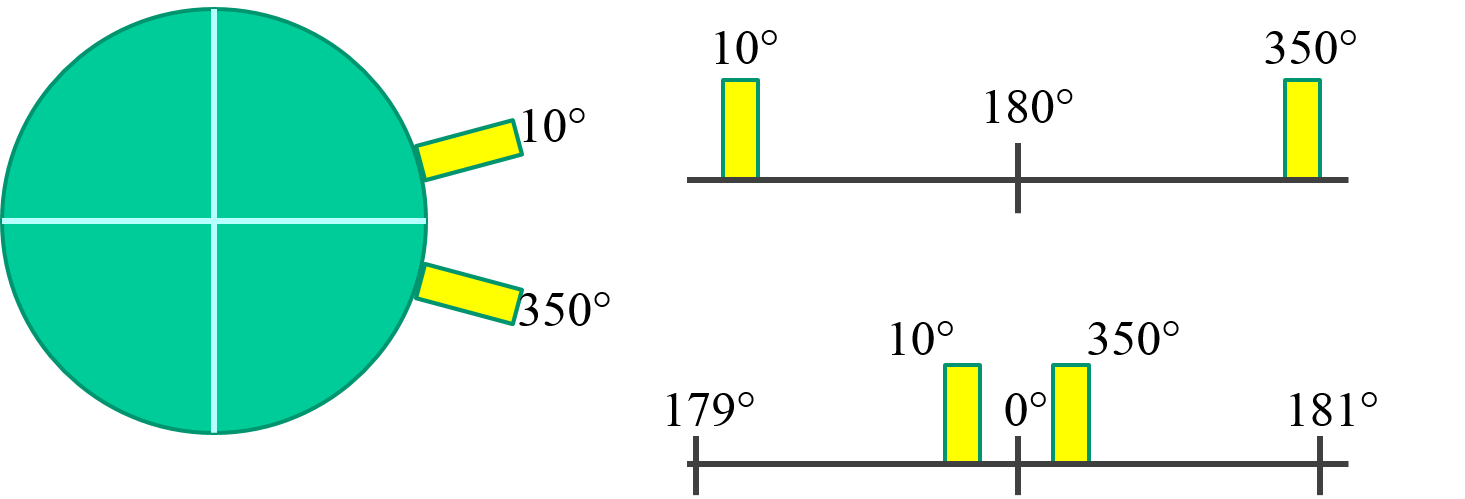
\includegraphics[width=4.30250in,height=1.46419in]{directional_histogram}
	\caption{Motivaci\'on de la estad\'istica de datos orientados. \textquestiondown Cu\'al es la media? \textquestiondown Y la desviaci\'on est\'andar?}
	\label{f:directionalHist}
\end{figure}

La soluci\'on a este problema lo proporciona la estad\'istica de datos orientados al hacer uso del c\'alculo vectorial. Con este enfoque los estad\'igrafos b\'asicos para datos circulares se definen de la siguiente manera \citep[ch. 2]{mardia_directional_2000} y est\'an implementados en el paquete \verb|circular| del software estad\'istico \verb|R|:

Supongamos que se tienen \(n\) datos, si cada orientaci\'on \(\theta_{i}\) se puede hacer corresponder con un vector unitario \(\mathbf{x}_{\mathbf{i}} = ( \cos\theta_{i},\sin\theta_{i} )\); entonces la direcci\'on media \(\overline{\theta}\) es la direcci\'on del vector resultante \(\mathbf{x}_{\mathbf{1}} + \ldots + \mathbf{x}_{\mathbf{n}}\). Las coordenadas cartesianas del centro de masa son \(( \overline{C},\ \overline{S} )\), donde

\begin{equation}
\overline{C} = \frac{1}{n}\sum_{j = 1}^{n}{\cos\theta_{j}},
\quad
\overline{S} = \frac{1}{n}\sum_{j = 1}^{n}{\sin\theta_{j}}
\end{equation}

Por lo tanto \(\overline{\theta}\) es la soluci\'on a las ecuaciones

\begin{equation}
\overline{C} = \overline{R}\cos\overline{\theta},
\quad
\overline{S} = \overline{R}\operatorname{sen}\overline{\theta}\end{equation}

Donde la longitud resultante media \(\overline{R}\) est\'a dada por

\begin{equation}
\overline{R} = \sqrt{{\overline{C}}^{2} + {\overline{S}}^{2}} \end{equation}

Observe que \(0 \leq \overline{R} \leq 1\). Si las direcciones \(\theta_{1},\ldots,\theta_{n}\) son muy cercanas entre s\'i, entonces \(\overline{R}\) ser\'a cercano a 1, pero si est\'a muy dispersas entonces \(\overline{R}\) ser\'a cercano a 0. Por lo tanto \(\overline{R}\) es una medida de \emph{concentraci\'on} de los datos. N\'otese que en la \emph{estad\'istica convencional} (o de \emph{datos no orientados}), la varianza nos proporciona una medida de \emph{dispersi\'on}, opuesto a la interpretaci\'on de \(\overline{R}.\) An\'alogo a la varianza convencional y otros estad\'igrafos pueden encontrarse en el cap\'itulo 2 de \cite{mardia_directional_2000}. Para datos esf\'ericos o datos direccionales en \(\mathbb{R}^{p}\), consulte el cap\'itulo 9 del mismo libro o el libro de \cite{fisher_statistical_1993}.

Supongamos que se ha especificado una direcci\'on (origen) y orientaci\'on (sentido de giro) inicial. Dos ejemplos de tal especificaci\'on son: 1) un plano cartesiano matem\'atico (\(X^{+} = 0,\ Y^{+} = 90\)), y 2) uno geogr\'afico (N=0$^\circ$, E=90$^\circ$). Entonces la funci\'on de distribuci\'on \(F\) para un \'angulo aleatorio \(\theta\) se define como la funci\'on en
\(\mathbb{R}\) dada por

\[F( x ) = \mathrm{\Pr}( 0 < \theta \leq x )\]

\[0 \leq x \leq 2\pi\]

y

 \(F( x + 2\pi ) - F( x ) = 1\)
\(- \infty < x < \infty\) 

La ecuaci\'on significa que cualquier arco de longitud \(2\pi\) tiene probabilidad 1 (ya que tal arco es la totalidad de la circunferencia del c\'irculo).

A diferencia de distribuciones en los reales, \(\mathbb{R}\),

\[{F( x )} = \infty, \qquad
{F( x )} = - \infty\]

Por definici\'on,

\[F( 0 ) = 0, \qquad
F( 2\pi ) = 1\]

Para una variable circular, una funci\'on \(f\) es la densidad de probabilidad de una funci\'on de distribuci\'on totalmente (absolutely) continua si y s\'olo si

\begin{itemize}
\item
  \(f( \theta ) \geq 0\) casi por doquier en
  \(( - \infty,\infty )\),
\item
  \(f( \theta + 2k\pi ) = f( \theta )\) casi por
  doquier en \(( - \infty,\infty )\) con \(k\mathbb{\in Z}\)
  (i.e., \(f\) es peri\'odica),
\item
  \(\int_{0}^{2\pi}{f( \theta )\text{d}} = 1\).
\end{itemize}

Las funciones de densidad uni y bidimensional de probabilidad param\'etricas para datos orientados m\'as comunes son:

\begin{table}[H]
	\centering
	\label{tab:directionalModels}
	\begin{tabular}{|r|l|}
\hline
von Mises &
$f( \theta;\mu,\kappa ) = \frac{1}{2\pi I_{0}( \kappa )}e^{\kappa\cos( \theta - \mu )}$ \\
\hline
Fisher &
$f( \theta,\ \phi;\alpha,\beta,\ \kappa ) = \frac{1}{4\pi\sinh( \kappa )}\exp
[ \kappa\lbrack \operatorname{sen}\theta\operatorname{sen}\alpha\cos( \phi - \beta ) + \cos\theta\cos\alpha \rbrack ] \sin\theta$
\\ \hline
	\end{tabular}
	\caption{Funciones de densidad de probabilidad para datos orientados. $0 \le \theta < 2\pi, \quad 0 \le \phi < \pi/2,\quad 0 \le \kappa < \infty$. Ver ec. 3.5.17 de \cite{mardia_directional_2000}, ec. 2.2.6 en la secci\'on 2.2.4 de \cite{jammalamadaka_topics_2001} y ec. 4.22 de \cite{fisher_statistical_1993}.}
\end{table}

La funci\'on de densidad de von-Mises es el an\'alogo a la funci\'on de densidad de probabilidad normal ya que tambi\'en consta de dos par\'ametros, es unimodal y sim\'etrica.

	\chapter{Modelaci\'on de dependencias mediante la teor\'ia de c\'opulas.}
\label{ch:copulaTheory}

La metodolog\'{i}a moderna para modelar dependencias estoc\'{a}sticas es la teor\'ia de c\'opulas. \'Esta ha demostrado m\'{a}s generalidad y versatilidad que el enfoque de regresi\'{o}n cl\'{a}sico (lineal, por ejemplo) para modelar dependencias.

Aunque la teor\'ia de c\'opulas no es una teor\'ia tan nueva \citep{sklar_fonctions_1959}, se han dado pocas aplicaciones pr\'acticas. Dentro de la industria petrolera se han hecho algunas aplicaciones para simular conjuntamente propiedades petrof\'isicas usando c\'opulas \citep{diaz-viera_stochastic_2006,diaz-viera_spatial_2012,diaz-viera_stochastic_2006-2,diaz-viera_stochastic_2005-1,diaz-viera_stochastic_2005,erdely_modeling_2011,erdely_joint_2012,erdely_trivariate_2012,erdely_nonparametric_2009,hernandez-maldonado_simulacion_2014,hernandez-maldonado_joint_2012,hernandez-maldonado_joint_2012-1,hernandez-maldonado_trivariate_2012} pero a\'un no se han hechos trabajos respecto a las propiedades de fractura.

Desde un punto de vista, las c\'opulas son funciones que unen o ``acoplan'' funciones de distribuci\'on multivariada a sus funciones de distribuci\'on marginal unidimensional. No existen modelos cl\'asicos que combinen de manera general datos orientados con datos no orientados por lo que con este trabajo se propondr\'an modelos que de manera adecuada tomen en cuenta la dependencia con la c\'opula, y a la vez respeten y reproduzcan las marginales.

\section{Generalidades}

?`Qu\'e relaci\'on existe entre una funci\'on de distribuci\'on multivariada, \(H\), y sus funciones de distribuci\'on marginal, \(F\) y \(G\)? La soluci\'on a este problema la dio \cite{sklar_fonctions_1959} al crear una nueva clase de funciones a las que llam\'o c\'opulas.

Para poder abordar adecuadamente la definici\'on de c\'opulas y el teorema de \cite{sklar_fonctions_1959} observemos primero algunas definiciones.

Sean \({S_{1},S}_{2} \subset \overset{\overline{}}{\mathbb{R}}\) y \(H:S_{1} \times S_{2}\mathbb{\rightarrow R}\). Si denotamos al \'infimo como ``\(\mathrm{\inf}\)'', y suponemos que \({a_{1} = \mathrm{\text{inf\ }}S}_{1}\), \(a_{2} = \mathrm{\inf}\ S_{2}\), decimos que \(H\) est\'a \emph{aterrizada} si \(H\left( x,a_{2} \right) = 0 = H\left( a_{1},y \right)\) para todo \(\left( x,y \right) \in S_{1} \times S_{2}\).De igual manera, si denotamos al supremo como ``\(\mathrm{\sup}\)'', y suponemos que \({b_{1} = \mathrm{\text{sup\ \ }}S}_{1}\) y \(b_{2} = \mathrm{\sup}\ S_{2}\), decimos que una funci\'on \(H\) tiene \emph{marginales}, y que las marginales de \(H\) son las funciones \(F\) y \(G\) dadas por

\(\mathrm{\text{Dom}}\ F = S_{1}\) y \(F\left( x \right) = H\left( x,b_{2} \right)\) para todo \(x \in S_{1}\)

\(\mathrm{\text{Dom}}\ G = S_{2}\) y
\(G\left( x \right) = H\left( b_{2},y \right)\) para todo
\(y \in S_{2}\)

\noindent
Donde ``\(\mathrm{\text{Dom}}\)'' denota el dominio de la funci\'on
correspondiente.

Sean \({S_{1},S}_{2} \subset \overset{\overline{}}{\mathbb{R}}\), y
\(B = \left\lbrack x_{1},y_{1} \right\rbrack \times \left\lbrack x_{2},y_{2} \right\rbrack\)
un rect\'angulo tal que todos sus v\'ertices est\'an en \(S_{1} \times S_{2}\). Una funci\'on \(H:S_{1} \times S_{2}\mathbb{\rightarrow R}\) es bi-creciente si,

\begin{equation}
    \Delta_{xy}H(x,y) := \Delta_{x} \left(\Delta_{y}H(x,y)\right)
    = H(x_2,y_2) - H(x_2,y_1) - H(x_1, y_2) + H(x_1, y_1) \ge 0
	\label{eq:monotoneContstraint2D}
\end{equation}

\textbf{Definici\'on. Subc\'opula.} Una subc\'opula bidimensional (o 2-subc\'opula) es una funci\'on \(C'\) con las siguientes caracter\'isticas:

\begin{enumerate}
\item
  \(\mathrm{\text{Dom}}C^{'} = S_{1} \times S_{2}\) donde \(S_{1}\) y
  \(S_{2}\) son subconjuntos de  \(\mathbb{I =}\left\lbrack 0,1 \right\rbrack\) que contienen al cero y a 1,
\item
  \(C'\) est\'a aterrizada y es bi-creciente.
\item
  Para cada \(u \in S_{1}\), \(C^{'}\left( u,1 \right) = u\); y para
  cada \(v \in S_{2}\), \(C^{'}\left( 1,v \right) = v\).
\end{enumerate}

\textbf{Definici\'on. C\'opula.} Una c\'opula bidimensional (\'o 2-c\'opula) es una 2-subc\'opula \(C\) tal que \(\mathrm{\text{Dom}}\ C = \mathbb{I}^{2}\).

\textbf{Teorema de \cite{sklar_fonctions_1959}.} Sea \(H\) una funci\'on de distribuci\'on con funciones marginales \(F\) y \(G\). Entonces existe una c\'opula \(C\) tal que para todo \(x,y \in \overset{\overline{}}{\mathbb{R}}\),

\begin{equation}
	H(x,y) = C(F(x),G(y))
	\label{eq:sklarTheorem}
\end{equation}

Si \(F\) y \(G\) son continuas, entonces \(C\) es \'unica, de otra manera \(C\) est\'a determinada de manera \'unica en \(\mathrm{\text{Ran}}\ F \times \mathrm{\text{Ran}}\text{\ G}\). Si \(C\) es una c\'opula y \(F\) y \(G\) son funciones de distribuci\'on, entonces la funci\'on \(H\) definida por la ecuaci\'on \autoref{eq:sklarTheorem} es una funci\'on de distribuci\'on conjunta con marginales \(F\) y \(G\).

En la teor\'ia cl\'asica de c\'opulas se suponen modelos param\'etricos tanto para \(H\) como para las marginales \(F\) y \(G\). Por ejemplo, \(F\) pudiera ser \textit{normal} con par\'ametros \(\mu\) y \(\sigma^{2}\); y \(G\) \textit{exponencial} con par\'ametro \(\lambda\), mientras \(H\) la distribuci\'on normal bivariada con sus correspondientes par\'ametros.

Los modelos param\'etricos son importantes en varios aspectos.
Por ejemplo, sus par\'ametros proveen una interpretaci\'on r\'apida del fen\'omeno en estudio.
Existen todo un cat\'alogo de modelos \citep{nadarajah_compendium_2016} que explican una gran variedad de fen\'omenos.
Cuando se tiene poca confianza en los datos \'o se cuenta con modelos hipot\'eticos, se pueden probar ciertos modelos param\'etricos.
Generalmente, son m\'as f\'aciles de implementar computacionalmente que los modelos no param\'etricos y m\'as r\'apidos.

Como complemento a los modelos param\'etricos se tienen los modelos no-param\'etricos. Estos \'ultimos son realmente \'utiles cuando la estructura de dependencia es m\'as compleja que relaciones mon\'otonas entre variables \'unicamente \citep{joe_dependence_2014}. En el caso de existir marginales con formas complicadas (no sim\'etricas, multimodales, etc.), entonces el enfoque param\'etrico puede ser aplicado a la distribuci\'on multivariada directamente.

El ejemplo m\'as simple de una c\'opula no param\'etrica es la c\'opula emp\'irica, que se puede definir de la siguiente manera \citep{deheuvels_fonction_1979,fermanian_weak_2004,berghaus_weak_2017,radulovic_weak_2017,bucher_empirical_2011,carnicero_non-parametric_2013}.
Dada una muestra \(\left\{ \left( x_{1},y_{1} \right),\ \ldots,\ \left( x_{n},y_{n} \right) \right\}\) de la funci\'on de distribuci\'on conjunta del vector aleatorio \(\left( X,Y \right)\); con sus correspondientes pseudo-observaciones obtenidas mediante la \autoref{e:empF}.
Entonces, la funci\'on de distribuci\'on c\'opula emp\'irica se define como,

\begin{equation}
	{\hat{C}}_{n}\left( u,v \right) = \frac{1}{n}\sum_{i = 1}^{n}{\mathbbm{1}(u_{i} \leq u,v_{i} \leq v)}
	\label{e:empCopC} % 'emp'irical 'cop'ula 'c'ontinous case
\end{equation}

\noindent
Para \(1 \leq i \leq n\) donde
\(\mathbbm{1}(a \leq b,c \leq d)\) si \(a \leq b\) y \(c \leq d\) y cero en otro caso, con \(a,b,c,d\mathbb{\in R}\).

La \autoref{e:empCopC} se puede reescribir de la forma de la \autoref{e:empCopI}:

\begin{equation}
	n\hat{C}_{n}( u,v) =
	\sum_{i = 1}^{n}
	\mathbbm{1}(u_{i} \leq u,v_{i} \leq v)
	\label{e:empCopI} % 'emp'irical 'cop'ula 'I'nteger case
\end{equation}

De esta manera $n\hat{C}_n$, de manera an\'aloga a la forma emp\'irica univariada (\autoref{e:empF}), puede ser almacenado como un arreglo bidimensional de enteros sin signo.
Esto conlleva a evitar errores de redondeo que se puedan propagar ya que, para $n$ grandes, digamos $n=1\e{6}$, lo normal en estos tiempos, $1/n=1\e{-6}=0.000001$.
Adem\'as, tambi\'en hay un ahorro considerable en la memoria de la computadora. Como ventaja adicional, ayuda a obtener visualizaciones m\'as sencillas del algoritmo num\'erico para almacenar los valores de la c\'opula emp\'irica.

Para encontrar cualquier valor $\hat{C}_n(u,v)$ simplemente se compara $(u,v)$ con los valores $(u_i, v_i)$ siguiendo la funci\'on indicador y de forma acumulativa 2-creciente (hacia la derecha y hacia la arriba).

\begin{figure}
	\centering
	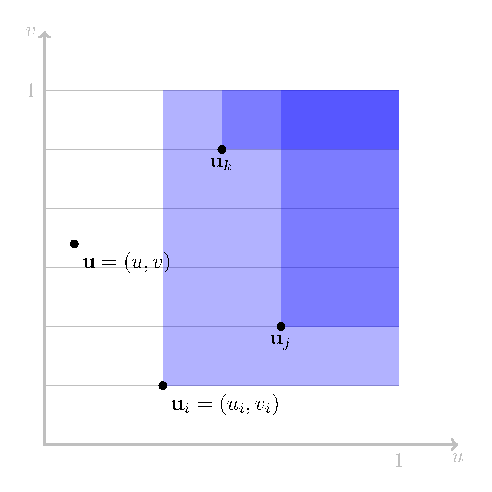
\includegraphics{empCopExplained}
	\caption{Donde $i,j,k \in \{1, \ldots,n\}$. Tonos m\'as oscuros representan valores de $n\hat{C}_n$ m\'as grandes. Cada cambio en tono representa una diferencia de uno (por la funci\'on indicador).}
	\label{f:empCopExplained}
\end{figure}

Esta forma permite un diagrama m\'as sencillo que relaciona la ubicaci\'on en el gr\'afico de pseudo-observaciones con su correspondiente arreglo en memoria de la computadora.
Supongamos que los datos $\{(x_i, y_i)\}$ est\'an ordenados por valores de $x$ crecientes, es decir, $u_i = u_{(i)}$. Esto no implica que $v_i = v_{(i)}$.
Adem\'as, suponemos que no hay valores repetidos.

\begin{figure}
	\centering
	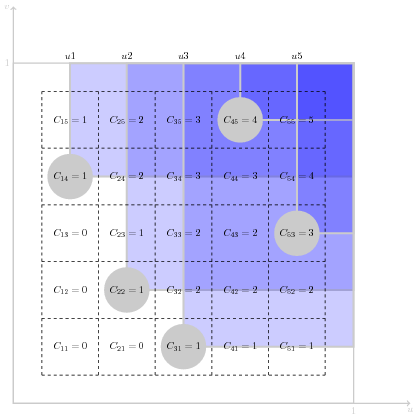
\includegraphics{empCopArray}
	\caption{Representaci\'on gr\'afica de la c\'opula emp\'irica y su relaci\'on con su almacenaje computacional en una matriz. El centro de cada c\'irculo representa una pseudo-observaci\'on $\mathbf{u}_i = (u_i,v_i)$. La malla regular de l\'ineas de guiones representa el arreglo en la memoria, $n\mathbf{C}$, que guarda los valores enteros $C_{ij}:=n\hat{C}_n(u_i, v_j)$. Donde $i$ denota el rengl\'on y $j$ la columna.
N\'otese que las $u_i$ est\'an ordenadas crecientemente pero no existe un orden en las $v_i$. Alternativamente se pudo haber ordenado por $v_i$ y dejar las $u_i$ sin orden.}
	\label{f:empCopArray}
\end{figure}

Para ligar la \autoref{f:empCopArray} con su correspondiente representaci\'on matricial $n\mathbf{C}$ (\autoref{e:empCopArray}), se referir\'a a la primera mediante palabras como horizontal/vertical, o paralelo al eje $u$/$v$; mientras que para referirse al correspondiente arreglo/matriz computacional se nombrar\'an renglones y columnas. Por ejemplo, el segundo rengl\'on de la matriz $n\mathbf{C}$, $n\mathbf{C}(2,\cdot)$, corresponde al rect\'angulo vertical de la \autoref{f:empCopArray} centrado en $u_2$, paralelo al eje $v$.

\begin{equation}
	n\mathbf{C} =
		\begin{pmatrix}
			C_{11} & C_{12} & C_{13} & C_{14} & C_{15}\\
			C_{21} & C_{22} & C_{23} & C_{24} & C_{25}\\
			C_{31} & C_{32} & C_{33} & C_{34} & C_{35}\\
			C_{41} & C_{42} & C_{43} & C_{44} & C_{45}\\
			C_{51} & C_{52} & C_{53} & C_{54} & C_{55}\\
		\end{pmatrix}
		=
		\begin{pmatrix}
			0 & 0 & 0 & 1 & 1\\
			0 & 1 & 1 & 2 & 2\\
			1 & 2 & 2 & 3 & 3\\
			1 & 2 & 2 & 3 & 4\\
			1 & 2 & 3 & 4 & 5
		\end{pmatrix}
	\label{e:empCopArray}
\end{equation}

Veamos el arreglo en la \autoref{f:empCopArray} por columnas, es decir, por rect\'angulos verticales de ancho $\Delta u_i$ y centrados en cada una de las pseudo-observaciones. 
N\'otese que, si fijamos un rengl\'on, digamos el rengl\'on $k$ que corresponde a $u_k$, los valores de $n\mathbf{C}$ satisfacen la siguiente relaci\'on de recurrencia:

\begin{equation}
	n\mathbf{C}(k,   ) =
	n\mathbf{C}(k-1, ) + \mathbf{v}_k
	\label{e:empCopRR}
\end{equation}

\noindent
donde el vector $\mathbf{v}_k := (0,0,\ldots,0,1,1,\ldots,1)$ contiene su primer $1$ en la entrada $rank(v_k)$, el rango de $v_k$.
Si $n \mathbf{C}$ fue inicializada con puros $0$, entonces se puede ahorrar memoria omitiendo la creaci\'on de un nuevo arreglo $\mathbf{v}_k$ al utilizar $n \mathbf{C}(k, ) := \mathbf{v}_n$.
Alternativamente, se puede proceder, primero por columnas y luego por renglones para obtener el mismo resultado.
La preferencia depender\'a del paradigma del arreglo en memoria del lenguaje de programaci\'on utilizado: \textit{row major} \'o \textit{column major}.
Tambi\'en se puede hacer m\'as eficiente al observar que el \'ultimo rengl\'on y la \'ultima columna tienen entradas correspondientes a $1,2,3,4,5$, para este caso. En el caso general tendr\'an entradas $1,2,\ldots,n$.
La implementaci\'on computacional de esta matriz se encuentra en la funci\'on \verb|bernsteincop::empCopM|, La funci\'on \verb|bernsteincop::genmat.copem| implementa un algoritmo similar pero no igual ya que compara los valores de $v_i$ en lugar de tomar el rango.

Para calcular el valor de la c\'opula emp\'irica en cualquier posici\'on $(u,v)$ solamente basta con saber los m\'aximos \'indices $i$ y $j$ que cumplen $(u_i,v_j) \le (u,v)$ elemento-a-elemento. Y $ \hat{C}_n(u,v) = n\mathbf{C}(i,j) / n$ (ver la \autoref{f:empCopExplained}).

N\'otese que la \autoref{e:empCopC} se puede escribir de la siguiente forma m\'as compacta y m\'as parecida a su contraparte univariada (\autoref{e:empF}):

\begin{equation}
	\hat{C}_{n}(\mathbf{u}) =
	\frac{1}{n} \sum_{i = 1}^{n}
	\mathbbm{1} (\mathbf{u}_{i} \leq \mathbf{u})
	\label{e:empCopV} % 'emp'irical 'cop'ula 'V'ectorized form
\end{equation}

\noindent
donde $\mathbf{u}_i := (u_i, v_i)$, $\mathbf{u}:=(u,v)$ y la relaci\'on de orden, $\le$, se efect\'ua componente a componente.


%Las c\'{o}pulas $C$ son funciones multivariadas, con ciertas caracter\'{i}sticas \citep[ch. 2]{nelsen_introduction_2006}, y que acoplan funciones de distribuci\'{o}n conjuntas $H$ y sus marginales univariadas $F_i$ de la siguiente manera para el caso bivariado \citep{sklar_fonctions_1959}:

%\begin{equation}
%\label{e:sklarT} % "e"quation of" Sklar" 's "T"heorem
%H(x_1,x_2)=C(F_1(x_1),F_2(x_2))
%\end{equation}

%De esta manera, la estructura de dependencia --capturada en la c\'{o}pula-- se puede modelar sin importar las funciones marginales univariadas.

Se puede ver que la c\'opula emp\'irica no es continua. Un modelo continuo de estructura de dependencia asociada dos variables aleatorias continuas e independientes $X$ y $Y$ es:

\begin{equation}
C_{XY}(u,v) = \Pi (u, v) := uv
\label{e:IndCop}
\end{equation}

Aunque la c\'opula emp\'irica no es continua, ella es \'util para obtener versiones continuas de la c\'opula.

\section{C\'opulas bivariadas de Bernstein}

Una versi\'on continua de la c\'opula emp\'irica se puede obtener mediante un ajuste polinomial. Una base del espacio de polinomios de grado $n$ son los polinomios de Bernstein (v\'ease la \autoref{s:bezier1D}):

\begin{equation}
	B(w|k,n):=\binom{k}{n} w^k (1 - w)^{n-k}
	\label{eq:bernsBasis}
\end{equation}

\noindent
donde $w \in [0,1]$, $k \in \{0,1, \ldots, n\}$.

Muchos lenguajes de programaci\'on tienen implementada eficientemente esta funci\'on, conocida en estad\'istica como la funci\'on de masa binomial. Por ejemplo, en \verb|R| est\'a implementada bajo el nombre \verb|dbinom|. Estos polinomios pueden ser utilizados para aproximar y suavizar la c\'opula emp\'irica (\autoref{e:empCopC}), lo que nos lleva a la c\'opula emp\'irica de Bernstein propuesta por \cite{sancetta_bernstein_2004}:

\begin{equation}
	C_B(u,v)=\sum_{i=0}^n \sum_{j=0}^n
	\hat{C}_n 
	\left(
	\frac{i}{n},\frac{j}{n}
\right)
B(u|i,n) B(v|j,n)
\end{equation}

En esta definici\'on, la c\'opula emp\'irica est\'a definida incluso para valores $u=0$, mientras que en la definici\'on de la funci\'on acumulativa emp\'irica (\autoref{e:empF}) la m\'inima pseudo-observaci\'on tomaba el valor $u_1 = 1/n$. Este inconveniente se resuelve a\~nadiendo $u_0 = 0$ \citep{sancetta_bernstein_2004} al vector de pseudo-observaciones emp\'iricas. Un ejemplo de la aplicaci\'on de esta teor\'ia en ciencias de la Tierra se muestra en la \autoref{f:phiK}.

\begin{figure}[H]
	\centering
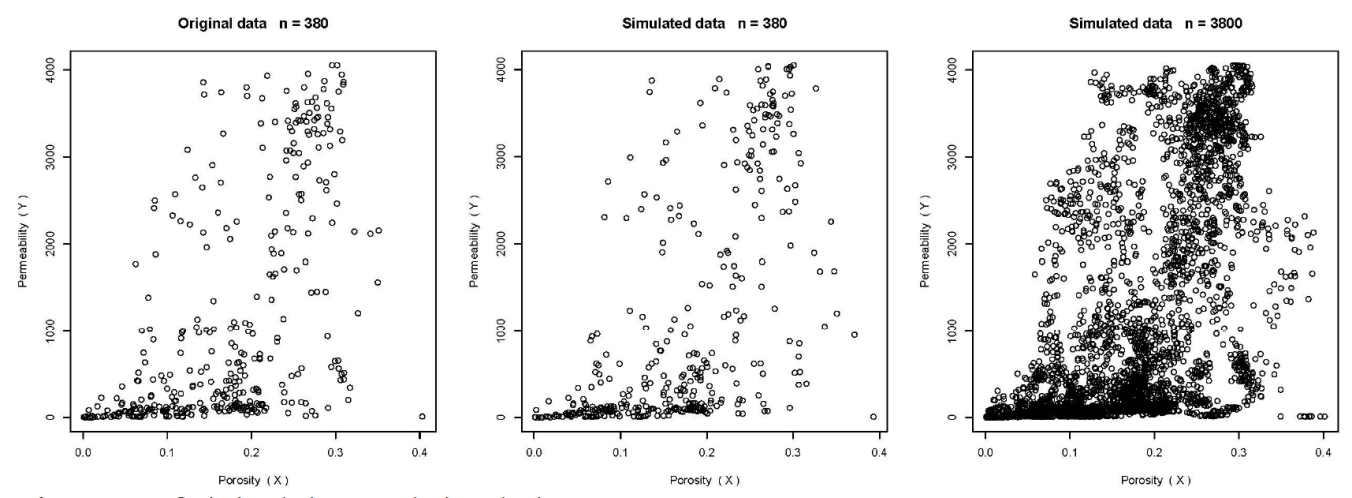
\includegraphics[width=6.14583in,height=2.26042in]{utb5}
	\caption{Ejemplo de la aplicaci\'on de la teor\'ia de c\'opulas de Bernstein \citep{erdely_joint_2012}.}
	\label{f:phiK}
\end{figure}

%donde \({\hat{C}}_{B}\left( \cdot , \cdot \right)\) es la c\'opula emp\'irica definida en la \autoref{e:empCopC}. N\'otese que a diferencia de otros autores \cite{nelsen_introduction_2006} esta definici\'on separa el grado del polinomio de la cantidad de datos, es decir, se puede tener una aproximaci\'on con un polinomio de menor grado, lo que conlleva a simulaciones computacionalmente m\'as r\'apidas.

Para obtener $C_B(u,v)$ se puede utilizar el algoritmo de de'Casteljau o se puede hacer mediante el uso del producto tensorial. Dado que hay suficientes trabajos describiendo el primer enfoque \citep{goldman_pyramid_2002,mann_blossoming_2006}, expliquemos el enfoque mediante tensores \citep{renteln_manifolds_2014} ya que permite una representaci\'on m\'as f\'acil para su implementaci\'on computacional.

\begin{equation}
	C_B(u,v) = \sum \mathbf{A}
\end{equation}	

\noindent
donde hemos definido la notaci\'on $\sum \mathbf{A}$ como la suma de todos los elementos del arreglo $\mathbf{A}$, la cual est\'a definida de la siguiente manera:

\begin{equation}
	\mathbf{A} = 
	\begin{pmatrix}
		\hat{C}(0,0)B(u|0,n)B(v|0,n)  & \hat{C}(0,1)B(u|0,n)B(v|1,n) & \cdots & \hat{C}(0,n)B(u|0,n)B(v|n,n)\\
		\hat{C}(1,0)B(u|1,n)B(v|0,n)  & \hat{C}(1,1)B(u|1,n)B(v|1,n) & \cdots & \hat{C}(1,n)B(u|1,n)B(v|n,n)\\
		\hat{C}(2,0)B(u|2,n)B(v|0,n)  & \hat{C}(2,1)B(u|2,n)B(v|1,n) & \cdots & \hat{C}(2,n)B(u|2,n)B(v|n,n)\\
		\vdots & \vdots & \ddots & \vdots \\
		\hat{C}(n,0)B(u|n,n)B(v|0,n)  & \hat{C}(n,1)B(u|n,n)B(v|1,n) & \cdots & \hat{C}(n,n)B(u|n,n)B(v|n,n)\\
	\end{pmatrix}
\end{equation}

\noindent
tambi\'en definimos $\hat{C}(i,j):= \hat{C}_n (i/n,j/n)$.

Existen varios factores repetidos que se pueden omitir si calculamos los siguientes vectores columna:

\begin{align}
	\mathbf{B}(u|n) &:= (B(u|0,n), B(u|1,n), \ldots, B(u|n,n))^T \\
	\mathbf{B}(v|n) &:= (B(v|0,n), B(v|1,n), \ldots, B(v|n,n))^T
	\label{eq:bernsteinsBasis}
\end{align}

\noindent
y haciendo el producto exterior (o producto tensorial) de dos vectores $\mathbf{a}$ y $\mathbf{b}$, denotado mediante $\mathbf{a} \otimes \mathbf{b}$, el cual produce un matriz $\mathbf{w}$ con coordenadas $w_{ij}= a_i b_j$. Si los vectores son vectores columna, $\mathbf{a} \otimes \mathbf{b}$ es equivalente a la multiplicaci\'on matricial $\mathbf{a}\mathbf{b}^T$. Un ejemplo particular se tiene si $\mathbf{a}=(1,2)^T \in \mathbb{R}^2$ y $\mathbf{b}=(3,4,5)^T \in \mathbb{R}^3$:

\begin{align}
	\mathbf{a} \otimes \mathbf{b}
	=
	\mathbf{a} \mathbf{b}^T
	&=
		\begin{pmatrix}
			a_1 \\ a_2
		\end{pmatrix}
		\begin{pmatrix}
			b_1 & b_2 & b_3
		\end{pmatrix}
	=
		\begin{pmatrix}
			a_1 b_1 & a_1 b_2 & a_1 b_3 \\
			a_2 b_1 & a_2 b_2 & a_2 b_3
		\end{pmatrix} \\
	&=
		\begin{pmatrix}
			1 \\ 2
		\end{pmatrix}
		\begin{pmatrix}
			3 & 4 & 5
		\end{pmatrix}
	=
		\begin{pmatrix}
			1 \cdot 3 & 1 \cdot 4 & 1 \cdot 5 \\
			2 \cdot 3 & 2 \cdot 4 & 2 \cdot 5
		\end{pmatrix}
	=
		\begin{pmatrix}
			3 & 4 & 5 \\
			6 & 8 & 10
		\end{pmatrix}
		\label{e:tensorProd2D}
\end{align}

Por lo tanto, $\mathbf{A}$ se puede reescribir de la siguiente manera:

\begin{equation}
	\mathbf{A}= \hat{\mathbf{C}} \odot [\mathbf{B}(u|n) \otimes \mathbf{B}(v|n)]
\end{equation}

\noindent
donde $\odot$ es el producto elemento-a-elemento de las matrices (tambi\'en conocido como el producto Hadamard o de Schur), y $\hat{\mathbf{C}}$ es la matriz c\'opula emp\'irica (\autoref{e:empCopArray}) cuyos elementos son $\hat{C}_n(u_i,v_j)$. N\'otese que tanto $\mathbf{B}(u|n) \otimes \mathbf{B}(v|n)$ como $\mathbf{\hat{C}}$ pertenecen a $\mathbb{M} ^{(n+1)\times(n+1)}$, las matrices de $(n+1)\times(n+1)$, $n+1$ renglones por $n+1$ columnas.

De esta forma, el c\'odigo computacional se puede hacer eficiente y f\'acil de leer:

\begin{equation}
	C_B(u,v) = \sum \left\{ \mathbf{\hat{C}} \odot [\mathbf{B}(u|n) \otimes \mathbf{B}(v|n)] \right\}
	\label{e:copBernComp}
\end{equation}

M\'as adelante, en la secci\'on de simulaci\'on, se requiere $\partial C_B / \partial u$, la que a su vez requiere las diferencias de primer orden con respecto a $u$ de la c\'opula emp\'irica, $\Delta_u \hat{C}_n$:
	
\begin{equation}
	\Delta_u \hat{C}_n
	\left( \frac{i}{n}, \frac{j}{n} \right)
	= \hat{C}_n
	\left(
		\frac{i+1}{n}, \frac{j}{n}
	\right)
	- \hat{C}_n
	\left(
		\frac{i}{n}, \frac{j}{n}
	\right)
	\label{e:forwardDiff2D}
\end{equation}

Para entender la representaci\'on matricial de la \autoref{e:forwardDiff2D}, a continuaci\'on se muestra un arreglo en el que cada entrada tiene la forma $C_{(i+1)j} - C_{ij}$.

\begin{equation}
\setlength\arraycolsep{8pt}
\Delta_u \mathbf{\hat{C}}=
	\begin{pmatrix}[2]
		C_{10}-C_{00} & C_{11}-C_{01} & C_{12}-C_{02} & \cdots & C_{1n} - C_{0n} \\
		C_{20}-C_{10} & C_{21}-C_{11} & C_{22}-12 & \cdots & C_{2n} - C_{1n} \\ 
		C_{30}-C_{20} & C_{31}-C_{21} & C_{32}-C_{22} & \cdots & C_{3n} - C_{2n} \\ 
		\vdots & \vdots & \vdots & \ddots & \vdots \\
		C_{n0}-C_{(n-1)0} & C_{n1}-C_{(n-1)1} & C_{n2}-C_{(n-1)2} & \cdots & C_{nn} - C_{(n-1)n} \\ 
	\end{pmatrix}
	\label{e:empCopDiffU}
\end{equation}

Este arreglo, se obtiene directamente del arreglo de la c\'opula emp\'irica (\autoref{e:empCopArray}) extendida mediante $C_{0i}=C_{i0}=0$.

\begin{equation}
\setlength\arraycolsep{8pt}
	\mathbf{\hat{C}} =
	\begin{pmatrix}[2]
		C_{00} & C_{01} & C_{02} & C_{03} & \cdots & C_{0(n-1)} & C_{0n}\\
		C_{10} & C_{11} & C_{12} & C_{13} & \cdots & C_{1(n-1)} & C_{1n}\\
		C_{20} & C_{21} & C_{22} & C_{23} & \cdots & C_{2(n-1)} & C_{2n}\\
		C_{30} & C_{31} & C_{32} & C_{33} & \cdots & C_{3(n-1)} & C_{3n}\\
		\vdots  & \vdots  & \vdots  & \vdots  & \ddots & \vdots & \vdots \\
		C_{(n-1)0} & C_{(n-1)1} & C_{(n-1)2} & C_{(n-1)3} & \cdots & C_{(n-1)(n-1)} & C_{(n-1)n}\\
		C_{n0} & C_{n1} & C_{n2} & C_{n3} & \cdots & C_{n(n-1)} & C_{nn}\\
		\end{pmatrix}
	\label{e:empCopArrayExt}
\end{equation}

N\'otese que mientras $\mathbf{\hat{C}} \in \mathbb{M}^{(n+1) \times (n+1)}$, $\Delta_u \mathbf{\hat{C}} \in \mathbb{M}^{n \times (n+1)}$. Al igual que el arreglo de la c\'opula emp\'irica, para ahorrar memoria y evitar errores de redondeo que se puedan propagar a trav\'es de lo c\'alculos, el arreglo $\Delta_u \mathbf{\hat{C}}$ se puede guardar como $\Delta_u n\mathbf{\hat{C}}$ (\autoref{e:empCopArray}).

Por otro lado, tambi\'en es \'util tener a la mano $\Delta_v \mathbf{\hat{C}}$, la diferencia finita de primer orden de la c\'opula emp\'irica con respecto a la segunda variable. En este caso se tiene que $\Delta_u \mathbf{\hat{C}} \in \mathbb{M}^{(n+1) \times n}$ y su arreglo tiene la forma de la \autoref{e:empCopDiffV}. 

\begin{equation}
\setlength\arraycolsep{8pt}
\Delta_v \mathbf{\hat{C}}=
	\begin{pmatrix}[2]
		C_{01}-C_{00} & C_{02}-C_{01} & C_{03}-C_{02} & \cdots & C_{0n} - C_{0(n-1)} \\
		C_{11}-C_{10} & C_{12}-C_{11} & C_{13}-C_{12} & \cdots & C_{1n} - C_{1(n-1)} \\ 
		C_{21}-C_{20} & C_{22}-C_{21} & C_{23}-C_{22} & \cdots & C_{2n} - C_{2(n-1)} \\ 
		C_{31}-C_{30} & C_{32}-C_{31} & C_{33}-C_{32} & \cdots & C_{3n} - C_{3(n-1)} \\ 
		\vdots & \vdots & \vdots & \ddots & \vdots \\
		C_{n1}-C_{n0} & C_{n2}-C_{n1} & C_{n3}-C_{n2} & \cdots & C_{nn} - C_{n(n-1)} \\ 
	\end{pmatrix}
	\label{e:empCopDiffV}
\end{equation}

Ahora, estamos preparados para definir las derivadas de la c\'opula de Bernstein \citep{phillips_interpolation_2003,sancetta_bernstein_2004}:

\begin{align}
	\partial C_B / \partial u
	&= \sum_{j=0}^n
	\left\{
		B(v|j,n) n 
		\left[
			\sum_{i=0}^{n-1} \Delta_u \hat{C}_n 
			\left(
				\frac{i}{n} , \frac{j}{n}
			\right)
			B(u|i,n-1)
		\right]
	\right\} \\
	&= n \sum_{i=0}^{n-1} \sum_{j=0}^n B(u|i,n-1) \Delta_u \hat{C}_n 
	\left(
		\frac{i}{n} , \frac{j}{n}
	\right)
	B(v|j,n) 
	\label{eq:bernsCopDerU}
\end{align}

Los sumandos de esta ecuaci\'on, al igual que para la c\'opula de Bernstein (\autoref{e:empCopArray}), se pueden escribir como elementos de la matriz de la \autoref{eq:empCopDiffUarray}:

\begin{equation}
	\begin{pmatrix}
		B(u|0,n-1)\Delta_u \hat{C}_n(0,0)B(v|0,n) & \cdots & B(u|0,n-1)\Delta_u \hat{C}_n(0,1)B(v|n,n) \\
		B(u|1,n-1)\Delta_u \hat{C}_n(\frac{1}{n},0)B(v|0,n) & \cdots & B(u|1,n-1)\Delta_u \hat{C}_n(\frac{1}{n},1)B(v|n,n) \\
		B(u|2,n-1)\Delta_u \hat{C}_n(\frac{2}{n},0)B(v|0,n) & \cdots & B(u|2,n-1)\Delta_u \hat{C}_n(\frac{2}{n},1)B(v|n,n) \\
		\vdots & \ddots & \vdots \\
		B(u|n-1,n-1)\Delta_u \hat{C}_n(\frac{n-1}{n},0)B(v|0,n) & \cdots & B(u|n-1,n-1)\Delta_u \hat{C}_n(\frac{1}{n},1)B(v|n,n) \\
	\end{pmatrix}
	\label{eq:empCopDiffUarray}
\end{equation}

Reutilizando la \autoref{eq:bernsteinsBasis} y la \autoref{e:empCopDiffU}, tenemos que

\begin{equation}
	\frac{\partial C_B}{\partial u}(u,v)
	= n \sum \left\{\Delta_u \mathbf{\hat{C}} \odot [\mathbf{B}(u|n-1) \otimes \mathbf{B}(v|n)] \right\}
	\label{e:copBernDiffComp}
\end{equation}

De manera similar tenemos:

\begin{equation}
	\frac{\partial C_B}{\partial v}(u,v)
	= n \sum \left\{\Delta_v \mathbf{\hat{C}} \odot [\mathbf{B}(u|n) \otimes \mathbf{B}(v|n-1)] \right\}
	\label{e:copBernDiffVComp}
\end{equation}

La funci\'on de densidad de c\'opula $c$ ($c$ min\'uscula) es la segunda derivada parcial con respecto a cada una de las variables. En el caso de la c\'opula de Bernstein, \'esta se puede escribir como \citep{carnicero_non-parametric_2013}:

\begin{equation}
	\hat{c}_{B} (u,v)
	= \sum_{i = 0}^{n} {\sum_{j = 0}^{n} p_{i j}}
	\beta \left( u|i,n-i+1 \right)
	\beta \left( v|j,n-j+1 \right)
	\label{eq:bernsCopDens2D}
\end{equation}

Donde

\begin{equation*}
	\beta (x|a,b) = \frac{1}{B(a,b)} x^{a-1} (1-x)^{b-1}
\end{equation*}

\noindent
Y donde los pesos son

\begin{equation}
	p_{ij} = \frac{1}{n}\sum_{k=1}^{n}
	\mathbbm{1}
	\left(
	\frac{i-1}{n} < u_k \le \frac{i}{n},
	\frac{j-1}{n} < v_k \le \frac{j}{n}
	\right)
	\label{eq:copWeights}
\end{equation}

\noindent
Para $i,j = 1,\ldots,n$.

Estos pesos son equivalentes al estimador del histograma en $[0,1]^2$ de la c\'opula (para m\'as detalle de dichos estimadores v\'ease \cite{scott_multivariate_1992}); es decir, $p_{ij}$  es $1/n$ veces el n\'umero de puntos $(u_i, v_i)$ dentro del rect\'angulo delimitado por el rect\'angulo $(i-1,i]/k \times (j-1,j]/k$ (v\'ease \autoref{fig:periodicCondition}).

\begin{figure}[H]
	\centering
	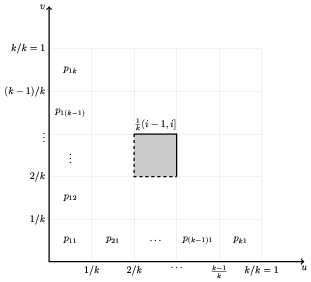
\includegraphics{periodicCondition}
	\caption{Representaci\'on esquem\'atica de los pesos $p_{ij}$ de la densidad de c\'opula.}
	\label{fig:periodicCondition}
\end{figure}

\cite{sancetta_bernstein_2004} y \cite{phillips_interpolation_2003} demuestran que el sesgo de los polinomios Bernstein de orden \(k\) es del orden de\(\ d \slash k + \mathcal{O}(1 \slash k)\) para alguna constante finita \(d\). Ellos tambi\'en proporcionan valores \'optimos para \(k\).

Recientemente el uso de splines penalizados se ha incorporado a la teor\'ia de c\'opulas no param\'etricas \cite{kauermann_flexible_2013}. En dicho trabajo se muestra las ventajas que tienen los splines penalizados sobre otros enfoques no param\'etricos como el de Bernstein, wavelets y kernel. \cite{kauermann_flexible_2013} aproximan la copula densidad, \(c\),

\[c\left( u_{1},\ldots,u_{p} \right) \approx \sum_{\mathbf{k}\mathcal{\in K}}^{}{b_{\mathbf{k}}\phi_{\mathbf{k}}\left( u_{1},\ldots,u_{p} \right)}\]

\noindent
Donde \(b_{\mathbf{k}}\) son los coeficientes y \(\phi_{\mathbf{k}}\)
son splines penalizados.

\section{C\'opulas bivariadas para vectores aleatorios con componentes orientadas}\label{s:copCirLin}

\cite{johnson_angular-linear_1978,wehrly_bivariate_1980} mostraron que la
funci\'on de distribuci\'on conjunta de una variable \(X\), y una
circular \(\Theta\), se puede expresar como

$$f_{\Theta,X}\left( \theta,x \right) = 2\pi g \{ 2\pi\left\lbrack F_{\Theta}\left( \theta \right) + F_{X}\left( x \right) \right\rbrack \} f_{\Theta}\left( \theta \right)f_{X}\left( x \right)$$

Donde \(g\left( \cdot \right)\) es una funci\'on de densidad de una
variable aleatoria circular. Por lo tanto, la copula para \(\Theta\) y
\(X\) debe satisfacer:

$$c\left( F_{\Theta}\left( \theta \right),F_{X}\left( x \right) \right) = 2\pi g\left( 2\pi\left\lbrack F_{\Theta}\left( \theta \right) + F_{X}\left( x \right) \right\rbrack \right)$$

Una de las aplicaciones de esta teor\'ia se ha hecho en la estimaci\'on de ozono en la ciudad de M\'exico \cite{fernandezduran_modelling_2004} usando sumas trigonom\'etricas no negativas para modelar la funci\'on de densidad de variables aleatorias circulares y c\'opulas circulares-lineales para modelar la dependencia conjunta. N\'otese que el enfoque de Fern\'andez-Dur\'an es un enfoque param\'etrico.

Otro caso de c\'opulas no param\'etricas de datos que incluyen datos circulares es la adaptaci\'on de \cite{carnicero_non-parametric_2013} a las c\'opulas de Bernstein de \cite{sancetta_bernstein_2004}. Dicha adaptaci\'on consiste en modelos propuestos para tomar en cuenta la periodicidad de los datos circulares.

La funci\'on de densidad de probabilidad \(f_{\Theta,X}\left( \cdot , \cdot \right)\) de un vector aleatorio \(\left( \Theta,X \right)\) es una funci\'on no negativa definida en la superficie de un cilindro \(\mathbb{S}^{1}\mathbb{\times R}\). Esta densidad tiene periodo \(2\pi\) en la componente circular:

\begin{equation}
	f_{\Theta,X}\left( \theta,x \right) = f_{\Theta,X}\left( \theta + 2k,x \right)
	\label{eq:periodiccondition}
\end{equation}

\noindent
para \(k \in \mathbb{Z}, -\infty < \theta < \infty\),

Y su integral es uno sobre un intervalo de longitud \(2\pi\) por los reales. Es decir, se integra a uno en todo su dominio.

Como consecuencia del teorema de \cite{sklar_fonctions_1959},

$$f_{\Theta,X}\left( \theta,x \right) = c\left( F_{\Theta}\left( \theta \right),F_{X}\left( x \right) \right)f_{\Theta}\left( \theta \right)f_{X}\left( x \right)$$

\noindent
donde \(c\left( \cdot , \cdot \right)\) es la densidad c\'opula.

Debido a la condici\'on de periodicidad para la funci\'on de distribuci\'on conjunta (\autoref{eq:periodiccondition}, es necesario que la c\'opula satisfaga:

\begin{equation}
	c\left( 0,v \right) = c\left( 1,v \right) \qquad \forall v \in [0,1]
	\label{eq:periodCop}
\end{equation}

Las c\'opulas de Bernstein no cumplen esta condici\'on, para la cual es necesario que los pesos de la \autoref{eq:copWeights}  satisfagan \(p_{1j_{2}} = p_{kj_{2}}\) para\(j_{2} = 1,\ldots,k\). Para remediarlo, \citet{carnicero_non-parametric_2013} proponen,

\begin{align}
	\tilde{p}_{1j_{2}} = {\tilde{p}}_{kj_{2}} = \frac{p_{1j_{2}} + p_{kj_{2}}}{2}  \qquad j_{2} &= 1,\ldots,k \label{eq:bernsWper}\\
	{\tilde{p}}_{j_{1}j_{2}} = p_{j_{1}j_{2}} \qquad j_{1} &\neq 1,k
\end{align}

Partiendo de la \autoref{fig:periodicCondition}, la correcci\'on de la \autoref{eq:bernsWper} equivale a promediar los vectores de pesos \verb|p[1,:]| y \verb|p[k,:]|. De manera visual, dicha correcci\'on se obtiene al promediar las dos celdas del mismo tono de gris en la \autoref{fig:periodicConditionCorrection}.

\begin{figure}
	\centering
	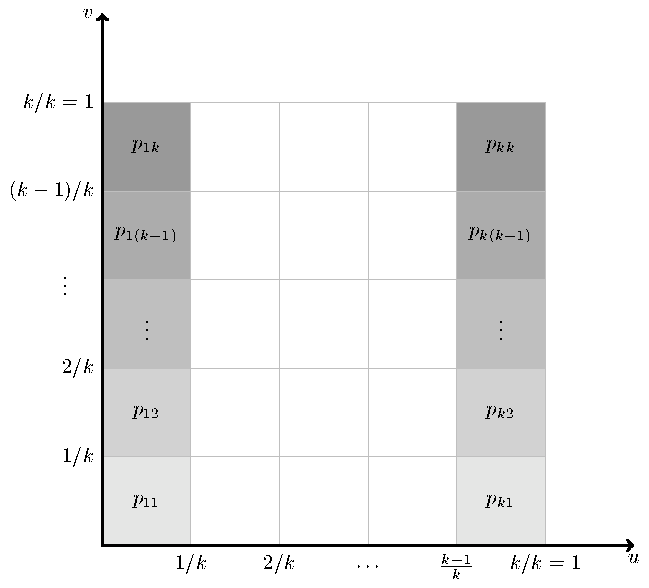
\includegraphics{periodicConditionCorrection}
	\caption{Correcci\'on para que la c\'opula de Bernstein cumpla con la condici\'on de periodicidad en la primera variable (\autoref{eq:periodCop}).}
	\label{fig:periodicConditionCorrection}
\end{figure}

Para validar el software desarrollado en \verb|R| se reprodujeron los resultados del art\'iculo de \citet{carnicero_non-parametric_2013} en el que se muestra la aplicaci\'on de esta metodolog\'ia a datos de direcci\'on del viento y precipitaci\'on pluvial. Para tal objetivo, se estimaron las funciones de densidad de probabilidad univariada para ambos datos. Para la direcci\'on del viento la funci\'on de densidad univariada fue una combinaci\'on de tres distribuciones de von Mises y para los datos de precipitaci\'on la funci\'on de densidad se compone de una combinaci\'on de tres exponenciales (\autoref{f:gijonDenCT}).

\begin{figure}
	\centering
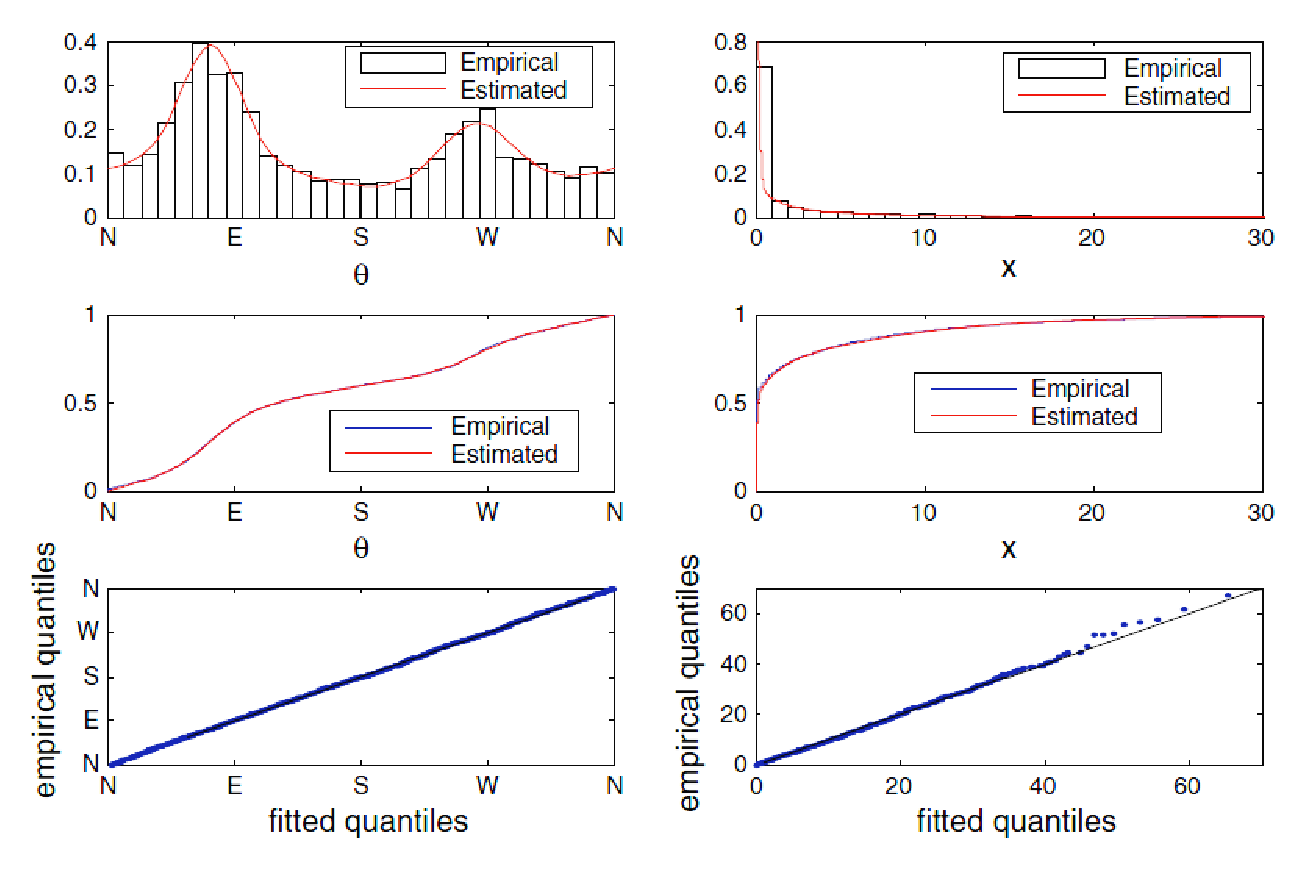
\includegraphics[width=5.01249in,height=3.32350in]{utb7}
	\caption{Densidad marginal estimada (top), funci\'on de distribuci\'on (medio) y gr\'aficos de cuantiles (abajo) para direcci\'on del viento (izquierda) y para la precipitaci\'on pluvial (derecha). Tomada de \cite{carnicero_non-parametric_2013}.}
	\label{f:gijonDenCT}
\end{figure}

Para estimar la funci\'on de densidad conjunta se utiliza la metodolog\'ia mostrada en esta secci\'on en lo que respecta a la parte bivariada. En la parte univariada aqu\'i proponemos que sea mediante los polonimos de Bernstein-Kantorovich, pero para reproducir los resultados de \citet{carnicero_non-parametric_2013} se utilizaron los modelos que ellos ajustaron. El resultado se muestra en la \autoref{f:gijonJointDens} y en la \autoref{f:gijonDenCT}. N\'otese que las marginales son claramente respetadas y la funci\'on de densidad es peri\'odica con respecto a la variable aleatoria orientada.

\begin{figure}[H]
	\centering
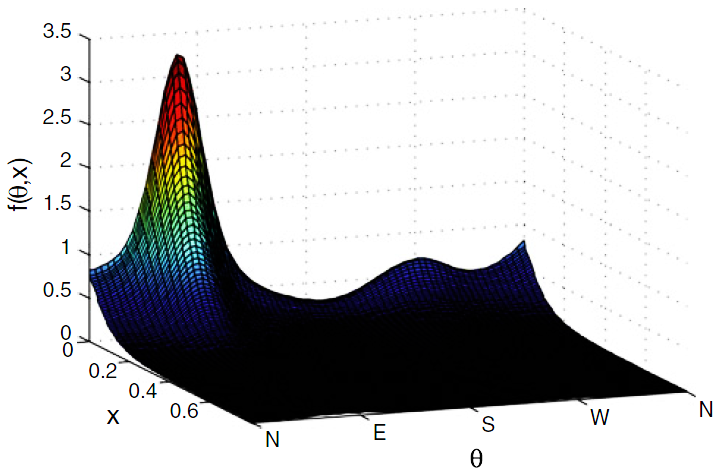
\includegraphics[width=3.75000in,height=2.47917in]{utb8}
	\caption{Funci\'on de densidad conjunta estimada (utilizando c\'opulas de Bernstein) de la variable circular-lineal \(\left( \Theta,X \right)\) . La cual describe la direcci\'on del viento y la precipitaci\'on pluvial.}
	\label{f:gijonJointDens}
\end{figure}

N\'otese que, aunque la correcci\'on propuesta por \citet{carnicero_non-parametric_2013} permite una c\'opula continua, no asegura diferenciabilidad, es decir, no asegura que la c\'opula sea suave en las fronteras. Una opci\'on m\'as vers\'atil que los polinomios de Bernstein que permite modelar curvas y sus derivadas al mismo tiempo son los splines. Dado que la suavidad se pide en la densidad, el enfoque de c\'opulas con splines propuesto por \citet{schellhase_density_2012} o el de Ferreira (2008 directional logspline) puede ser \'util para una aproximaci\'on m\'as natural en el caso de vectores aleatorios con componentes circulares.

%\section{C\'opulas no param\'etricas para datos circulares-circulares}\label{s:copParDir}

Hasta este momento solamente se ha estudiado el caso con una sola componente circular, pero m\'as es posible. En el caso bivariado, se puede hacer que ambas componentes sean circulares.

La funci\'on de densidad de probabilidad \(f_{\Theta_{1},\Theta_{2}}\left( \cdot , \cdot \right)\) de un vector aleatorio circular-circular \(\left( \Theta_{1},\Theta_{2} \right)\) es una funci\'on no negativa definida en la superficie de un toro, \(\mathbb{S}^{1} \times \mathbb{S}^{1}\). Esta densidad tiene periodo \(2\pi\) en ambas componentes:

\begin{equation}
f_{\Theta_{1},\Theta_{2}}\left( \theta_{1},\theta_{2} \right) = f_{\Theta_{1},\Theta_{2}}(\theta_{1} + 2j\pi,\theta_{2} + 2k\pi), \qquad j,k\mathbb{\in Z}, - \infty < \theta_{1},\theta_{2} < \infty 
\label{eq:den2Dcir}
\end{equation}
Y su integral es uno sobre el producto de dos intervalos de longitud \(2\pi\). Es decir, es uno al integrar sobre todo su dominio.

Debido a la condici\'on (\autoref{eq:den2Dcir}) para la funci\'on de distribuci\'on conjunta, es necesario que la c\'opula para datos circulares-circulares, adem\'as de la \autoref{eq:periodCop}, satisfaga:

\begin{equation}
	c(u,0) = c(u,1) \qquad \forall u \in [0,1]
	\label{eq:periodCondition2D}
\end{equation}

En el caso de las c\'opulas de Bernstein, los pesos son similares a la \autoref{eq:copWeights} salvo que las dos variables aleatorias correspondientes son circulares.
Por lo tanto los pesos tienen que satisfacer $p_{1j_{2}} = p_{kj_{2}}\) y \(p_{j_{1}1} = p_{j_{1}k}$ para $j_{1},j_{2} = 1,..,k$.
Y la correcci\'on de periodicidad, adem\'as de aplicarse a la primera variable $u$, posteriormente tiene que aplicarse a la segunda variable $v$. Lo que produce los siguientes pesos:

\({\tilde{p}}_{1j_{2}} = {\tilde{p}}_{kj_{2}} = \frac{p_{1j_{2}} + p_{kj_{2}}}{2}\)

\({\tilde{p}}_{j_{1}1} = {\tilde{p}}_{j_{1}k} = \frac{p_{j_{1}1} + p_{j_{1}k}}{2}\)

\({\tilde{p}}_{11} = {\tilde{p}}_{1k} = {\tilde{p}}_{k1} = {\tilde{p}}_{\text{kk}} = \frac{p_{11} + p_{1k} + p_{k1} + p_{\text{kk}}}{4}\)

Y \({\tilde{p}}_{j_{1}j_{2}} = p_{j_{1}j_{2}}\) para \(j_{1} \neq 1,k\)
y \(j_{2} \neq 1,k\) 

Lo que garantiza que la c\'opula se continua y peri\'odica en ambas variables.

Para ilustrar la metodolog\'ia, \cite{carnicero_non-parametric_2013} muestra la aplicaci\'on de esta metodolog\'ia a datos de direcci\'on dos boyas en el mar. Para tal objetivo, se estimaron las funciones de densidad de probabilidad univariada para ambos datos. En ambas variables, la funci\'on de densidad univariada fue una combinaci\'on de tres distribuciones de von Mises (\autoref{f:marginalDir}).

\begin{figure}[H]
	\centering
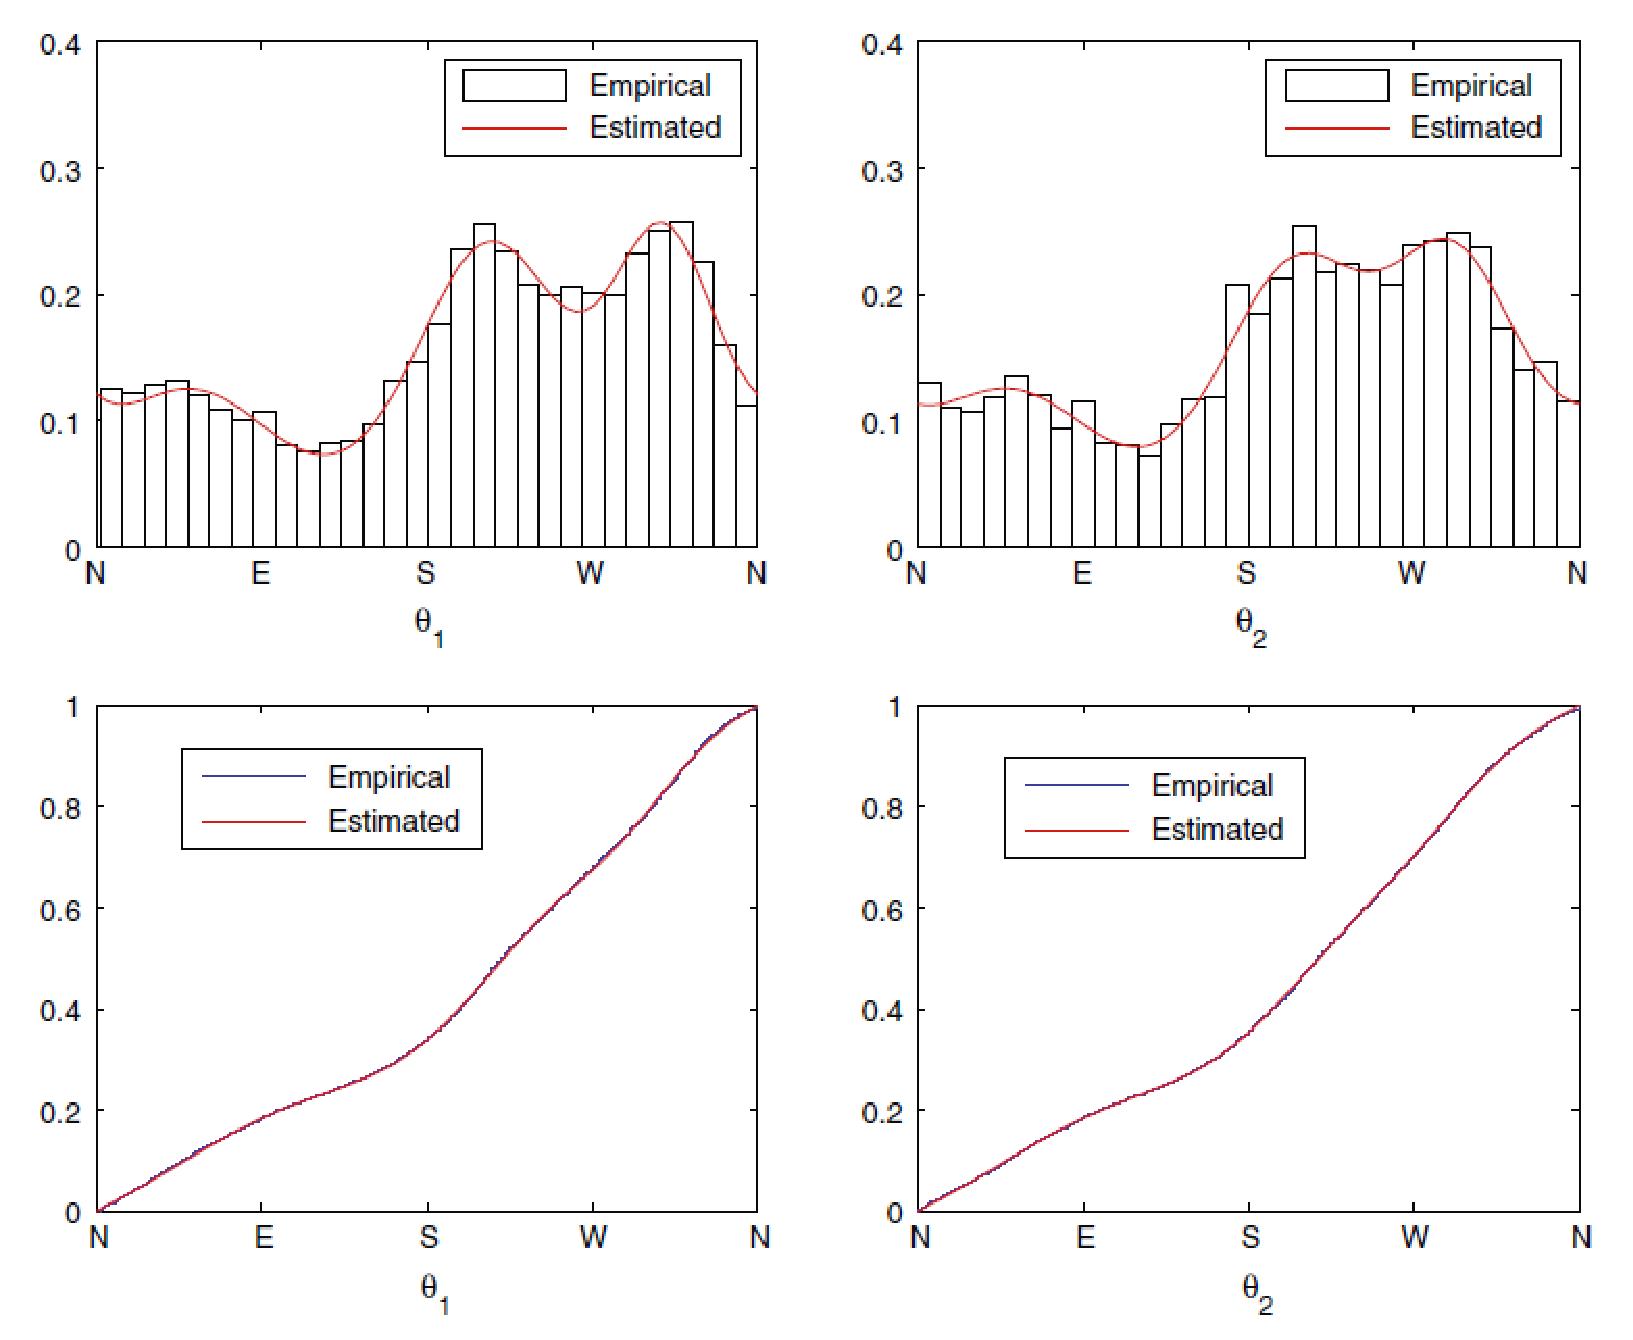
\includegraphics[width=4.82292in,height=3.93750in]{utb9}
	\caption{Densidad marginal estimada (top) y funci\'on de distribuci\'on (abajo) para la direcci\'on de dos boyas.}
	\label{f:marginalDir}
\end{figure}

\section{Simulaci\'on conjunta de variables aleatorias: caso bivariado}\label{s:simAlg2D}

Dado un modelo de dependencia (c\'opula), uno de los objetivos perseguidos al modelar la funci\'on de densidad de probabilidad conjunta es simular valores de las variables aleatorias.
Para simular datos a partir de la c\'opula se utiliza una variante del m\'etodo de distribuci\'on condicional \citep{nelsen_introduction_2006} en el cual se utiliza un enfoque no param\'etrico \citep{erdely_nonparametric_2009,erdely_joint_2012}:

\begin{enumerate}
\item
  Genere dos variables aleatorias \(u\) y \(t\) que sean independientes   y continuas en \(\left( 0,1 \right)\).
\item
  Obtenga \(v = c_{u}^{\left( - 1 \right)}\left( t \right)\). Donde
  \(t = c_{u}\left( v \right) = \frac{\partial\tilde{C}\left( u,v \right)\ }{\partial u}\)
  y \(c_{u}^{\left( - 1 \right)}\) es la inversa generalizada (\autoref{e:generalizedInv}) de \(c_{u}\).
\item
	Los datos simulados, \(\left( x,y \right)\), se obtienen utilizando   funciones cuantiles no param\'etricas de \(X\) y \(Y\) respectivamente.   Estas funciones \(\tilde{Q}\) y \(\tilde{R}\) son estimadas mediante   polinomios de Bernstein-Kantorovich \citep{munoz-perez_estimating_1987}. Por lo tanto   \(\left( x,y \right) = \left( \tilde{Q}\left( u \right),\tilde{R}\left( v \right) \right)\).
\end{enumerate}

Atendiendo al punto 1 de esta metodolog\'ia es necesario simular valores con una distribuci\'on uniforme en el intervalo \(\left\lbrack 0,1 \right\rbrack\), ya que estos son requeridos por la c\'opula. Esto se puede conseguir con la funci\'on \verb|stats::runif|. Recu\'erdese que la c\'opula bivariada tiene dominio \(\left\lbrack 0,1 \right\rbrack^{2}\).
Para el segundo paso se requieren a) la  derivada parcial de la c\'opula; b) obtener una funci\'on inversa.
En el caso de la c\'opula de Bernstein la derivada est\'a dada por la \autoref{eq:bernsCopDerU}.
Al terminar este segundo paso se cuenta con dos valores $u_i$ y $v_i$ que est\'an distribuidos uniformemente pero que conservan la misma dependencia que los datos originales.
Por \'ultimo, estos valores son los argumentos de las funciones cuantiles para obtener $x_i$ y $y_i$. 
La implementaci\'on computacional de estas funciones cuantiles se encuentra en el paquete \verb|lmomco| bajo el nombre de \verb|dat2bernqua|.
La \autoref{f:phiKhist} muestra un ejemplo de un conjunto de datos a los cuales se les model\'o su funci\'on de distribuci\'on con los polinomios de Bernstein-Kantorovich. Por lo tanto
$(x_{i},y_{i}) = (\tilde{Q}(u_{i}), \tilde{R}(v_{i}))$.

\begin{figure}[H]
	\centering
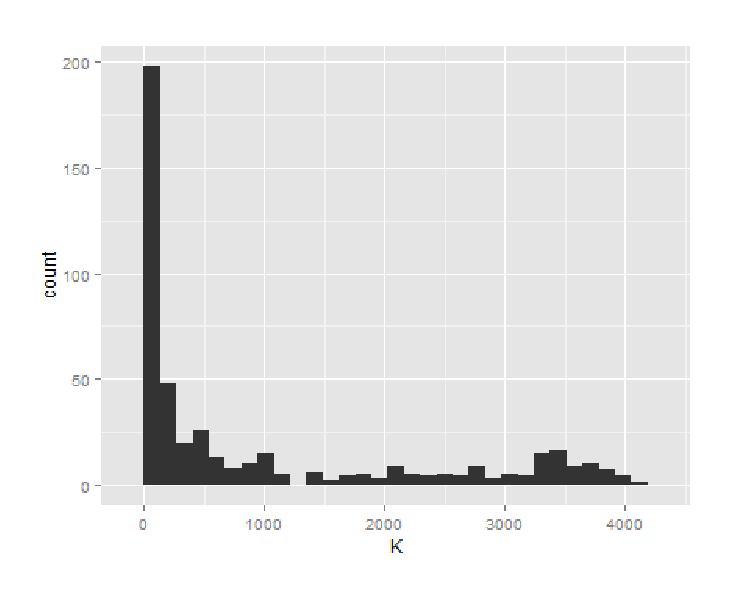
\includegraphics[width=2.82000in,height=2.24000in]{utb13}
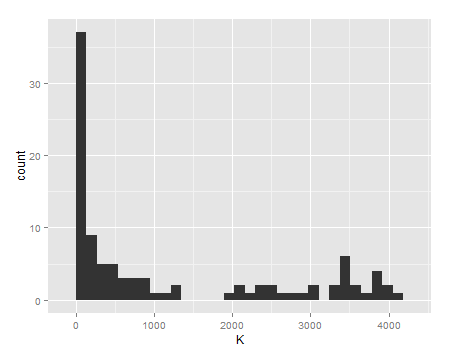
\includegraphics[width=2.82000in,height=2.24000in]{utb14}
\caption{Histogramas de un ejemplo de simulaci\'on no param\'etrica. 473 datos (izquierda) y 100 datos simulados (derecha).}
\label{f:phiKhist}
\end{figure}

\section{Simulaci\'on conjunta de variables aleatorias: caso multivariado}

Uno de los objetivos al modelar vectores aleatorios es generar muestras estad\'{i}sticamente equivalentes a los datos observados para as\'{i} poder cuantificar incertidumbre. Para lograr este cometido, se ilustra el algoritmo de simulaci\'{o}n.

El algoritmo de simulaci\'{o}n se simplifica si todas las $d$ marginales unidimensionales se distribuyen uniformemente lo cual se logra obteniendo la funci\'{o}n de distribuci\'{o}n acumulada de los datos ya que $F_i(x_i) \sim Uniforme(0,1)$. La generalidad del algoritmo se recupera al mapear cada marginal $u_{i} := F(x_i)$ en su variable correspondiente $x_{i}$ mediante el m\'etodo de la transformada inversa \citep[sec. 2.1.2, pp. 44]{robert_introducing_2009} utilizando la inversa generalizada (\autoref{e:generalizedInv}.

Para obtener una muestra simulada se procede con el siguiente algoritmo recursivo (\citeauthor{mai_simulating_2012}, \citeyear{mai_simulating_2012}, sec. 5.3.2, pp. 208;\citeauthor{dismann_statistical_2010}, \citeyear{dismann_statistical_2010}):

\begin{align}
	\text{inicio:} \qquad  W_{i} & \overset{i.i.d.}{\sim} Uniforme(0,1), \qquad \forall i \in \{1, \ldots, d\} \\
	\text{posteriormente:} \qquad U_{1} &:= W_{1} \\
U_{2} &:= F_{2|1}^{-}(W_{2}|U_{1}) \\
U_{3} &:= F_{3|2,1}^{-}(W_{3}|U_{2}, U_{1}) \\
% todo: insert vertical dots (ellipsis) here
U_{d} &:= F_{d|d - 1, \ldots, 1}^{-}(W_{d}|U_{d-1}, \ldots, U_{1})
\label{e:CopSimAlg_multi}
\end{align}

En el caso de teor\'ia de c\'opulas cada $F^{-}_{i|i-1,\ldots,1}$ es la inversa generalizada de la \autoref{e:CondDistVine}.

\section{Vine c\'{o}pulas: Caso trivariado}

Es bien sabido que el an\'{a}lisis y visualizaci\'{o}n bivariado de datos es m\'{a}s f\'{a}cil que el caso multivariado. Esto tambi\'en se cumple en el caso de la modelaci\'{o}n de dependencias mediante c\'{o}pulas. Un enfoque que permite estudiar dependencias con $d \ge 3$ mediante descomposiciones bivariadas es el conocido como Vine copulas (tambi\'en conocido como construcciones de c\'{o}pulas mediante pares).

El siguiente caso trivariado ilustra c\'{o}mo se efect\'{u}a la descomposici\'{o}n en pares a partir de la funci\'{o}n de densidad conjunta $f_{123}$ \citep{diaz2015vine}:

\begin{align}
f_{123} &= f_{23|1} \cdot f_1 \\
 &=c_{23|1} (F_{2|1}, F_{3|1}) \cdot f_{2|1} \cdot f_{3|1} \cdot f_1 \\
 &=c_{23|1} (F_{2|1}, F_{3|1}) \cdot \frac{f_{12}}{f_1} \cdot \frac{f_{13}}{f_1} \cdot f_1 \\
 &=c_{23|1} (F_{2|1}, F_{3|1}) \cdot c_{12}(F_1, F_2) \cdot c_{13}(F_1, F_3) \cdot f_1 \cdot f_2 \cdot f_3
\label{e:vine3}
\end{align}

N\'{o}tese que para la misma densidad $f_{123}$ existen otras dos posibles descomposiciones dependiendo de la variable condicionante.

Cada uno de los argumentos de las c\'opulas bivariadas de la descomposici\'on Vine (ecuaci\'on \ref{e:vine3}) est\'a dado como \citep{mai_simulating_2012,aas_pair-copula_2009,dismann_statistical_2010}:
%(\citeauthor{mai_simulating_2012}, \citeyear{mai_simulating_2012}, pp. 189, eq. 5.7). 
%; \citeauthor{gijbels_conditional_2011}, \citeyear{gijbels_conditional_2011}

\begin{equation}
F(x| \mathbf{x}) = \frac{\partial C_{X,X_j|\mathbf{X}_{-j}}
(F(x|\mathbf{x}_j), F(x_j|\mathbf{x}_{-j})}
{F(x_j|\mathbf{x}_{-j})}
\label{e:CondDistVine}
\end{equation}

\noindent
donde $\mathbf{x} \subset \{x_1, \ldots, x_d \}$, $\mathbf{x}^c:= \{x_1,\ldots, x_d\} - \mathbf{x}$, $x \notin \mathbf{x}$  y $x_j \notin \mathbf{x}_j \subset \mathbf{x}$.

N\'{o}tese que en la ecuaci\'{o}n (\ref{e:CondDistVine}) se utilizan may\'{u}sculas para denotar variables aleatorias mientras que las min\'{u}sculas denotan observaciones (realizaciones). La notaci\'{o}n tambi\'en distingue entre escalares ($x$ \'{o} $X$) y vectores ($\mathbf{x}$).

Para el caso trivariado se tiene \citep[pp. 209, example 5.7]{mai_simulating_2012} 

\begin{equation}
F(u_3| u_1,u_2) = \frac{\partial C_{3,1|2}
(F(u_3|u_2), F(u_1|u_2)}
{\partial F(u_1|u_2)}
\label{e:CondDistVine3}
\end{equation}

Un caso particular de las c\'opulas de Vine se tiene haciendo el \textit{supuesto de simplificaci\'on} \citep{joe_dependence_2014,gijbels_conditional_2011}

\begin{equation}
C_{3,1|2} = C_{3,1}
\label{e:simpAssum} % simplifying assumption
\end{equation}

Un caso m\'as particular pero frecuente se tiene si $U_3 \perp U_1 | U_2$ (ver \ref{e:IndCop}):

\begin{equation}
C_{3,1|2} (u,w) = uw
\label{e:CondInd} % conditionally independent copula
\end{equation}

Utilizando \ref{e:CondInd} en \ref{e:CondDistVine3} se tiene:

\begin{equation}
\frac{\partial C_{3,1|2}}{\partial F(u_1|u_2)} = F(u_3|u_2)
\label{e:marginalInd} % Marginally independent
\end{equation}

Lo que reduce el tiempo de c\'omputo para la simulaci\'on.

%N\'{o}tese que a cada par $F_{x|x} -- C_{x}$ correspondiente a la ecuaci\'{o}n MISSING, en el \'{a}rbol, se cuenta con dos argumentos de entrada (n\'{o}dos-hijos) y un argumento de salida $u_{i}$.
%
%En el \'{a}rbol se distingue entre nodo-hijo izquierdo y derecho. N\'{o}tese que en este caso particular, los nodos-hijos izquierdos corresponden con valores $w_{i}$.
%
%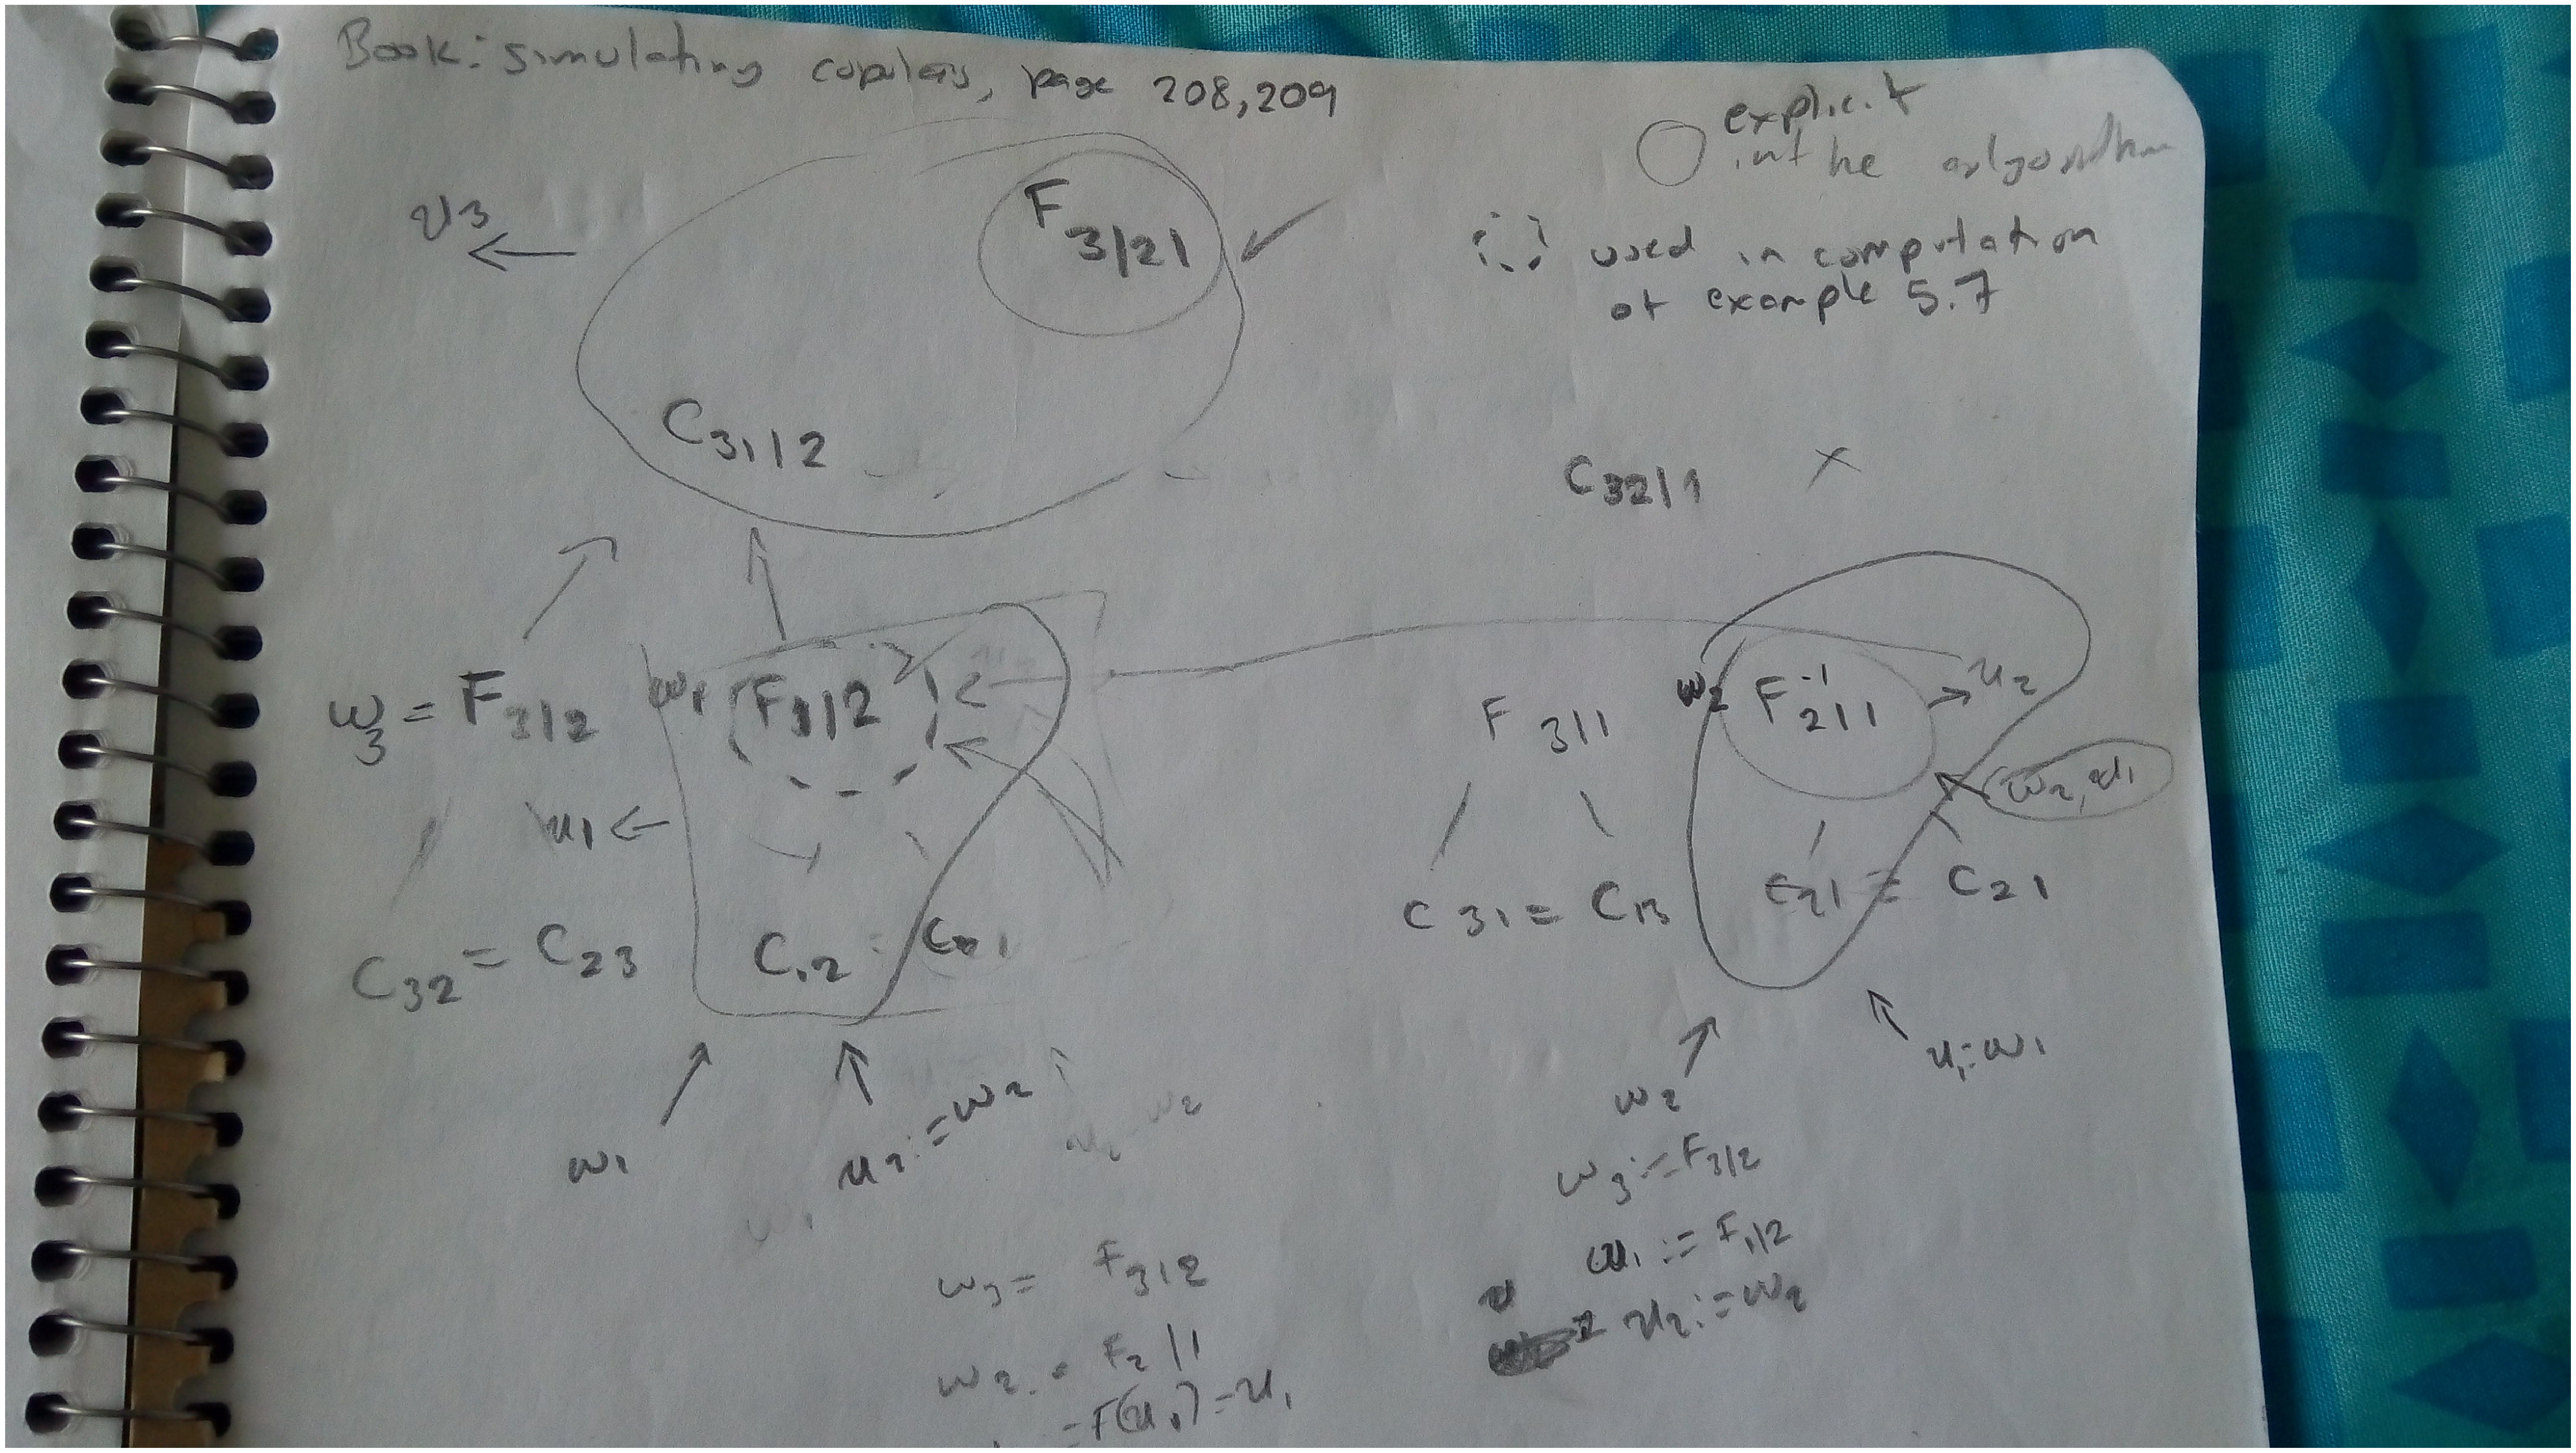
\includegraphics[width=0.9\textwidth]{SimTree}

\section{C\'{o}pulas de Bernstein: caso general multivariado}
 
%Una de las bases para aproximar funciones son los polinomios de Bernstein que en el caso univariado tienen la siguiente forma \citep{sancetta_bernstein_2004}: 
%\begin{equation}
%P_{v}^{m}(u) = \binom{m}{v} u^{v} (1 - u)^{m-v}
%\label{e:BernPoly1D}
%\end{equation}

%Estas funciones base ya han sido utilizadas dentro de la estad\'istica al aproximar funciones cuantiles \citep{munoz-perez_estimating_1987} y de manera aplicada en la simulaci\'on \citep{hernandez-maldonado_joint_2012,hernandez-maldonado_joint_2012-1,hernandez-maldonado_trivariate_2012,erdely-ruiz_modeling_2011,erdely_nonparametric_2009,diaz2015vine}. Este enfoque es no param\'etrico y se utilizar\'a para modelar las funciones de distribuci\'on marginales en este trabajo.

En el caso multivariado, para modelar dependencias, una aproximaci\'{o}n de una funci\'{o}n $d$-dimensional utilizando los polinomios de Bernstein toma la siguiente forma:

\begin{equation}
	G(u_1, \ldots, u_d) =
	\sum_{v_1 = 0}^{m_1} \dots \sum_{v_d = 0}^{m_d}
	\alpha
	\left(
		\frac{v_1}{m_1}, \ldots, \frac{v_d}{m_d}
	\right)
	\prod_{i = 1}^{d} B(u_i|v_i,m_i)
\label{e:BernPoly}
\end{equation}

Si definimos los arreglos ordenados (vectores) $n$-dimensionales

\begin{align}
	\mathbf{m} & := (m_1, \dots, m_n) \\
	\mathbf{u} & := (u_1, \ldots, u_n) \\
	\mathbf{v} & := (v_1, \ldots, v_n) \\
	\mathbf{0} & := (0, \ldots, 0)
\end{align}

entonces podemos definir

\begin{equation}
	\sum_{\mathbf{v} = \mathbf{0}}^{\mathbf{m}} := 
	\sum_{v_1 = 0}^{m_1} \dots \sum_{v_d = 0}^{m_d}
\end{equation}

y por lo tanto la ecuaci\'on (\ref{e:BernPoly}) se puede expresar como

\begin{equation}
	G(\mathbf{u}) =
	\sum_{\mathbf{v} = \mathbf{0}}^{\mathbf{m}}
	\alpha
	\left(
		\frac{v_1}{m_1}, \ldots, \frac{v_d}{m_d}
	\right)
	\prod_{i = 1}^{d} B(u_i|v_i,m_i)
\end{equation}

El caso m\'as sencillo se obtiene cuando $n=1$:

\begin{equation}
	G(u) = \sum_{v=0}^m
	\alpha
	\left(
		\frac{v}{m}
	\right)
	B(u|v,m)
\end{equation}

Dado que los polinomios satisfacen de manera natural muchas de las propiedades de las funciones de distribuci\'{o}n acumulada, los polinomios de Bernstein han demostrado ser una buena aproximaci\'{o}n de la c\'{o}pula emp\'{i}rica, que en el caso bivariado toma la siguiente forma \citep{deheuvels_fonction_1979}:

Para las simulaciones es importante tener la derivada de (\ref{e:BernPoly}), lo cual se puede obtener haciendo uso de \ref{e:bernCopDer}:  

\begin{align} \label{e:bernCopDer} % Bernstein copula derivative
	\frac{\partial G}{\partial u_l} &=
	\frac{\partial }{\partial u_l}
	\left[
		\sum_{v_1 = 0}^{m_1} \dots \sum_{v_l = 0}^{m_l}
		\dots \sum_{v_d = 0}^{m_d}
		\alpha
		\left(
			\frac{v_1}{m_1}, \ldots,
			\frac{v_l}{m_l}, \ldots,
			\frac{v_d}{m_d}
		\right)
		\prod_{i = 1}^{d} B(u_i|v_i,m_i)
	\right] \\
	&= 
		\sum_{v_1 = 0}^{m_1} \dots \sum_{v_d = 0}^{m_d}
		\prod_{i \ne l} B(u_i|v_i,m_i)
		\frac{\partial }{\partial u_l}
	\left[
		\sum_{v_l = 0}^{m_l}
		\alpha
		\left(
			\frac{v_1}{m_1}, \ldots,
			\frac{v_d}{m_d}
		\right)
		B(u_l|v_l,m_l)
	\right] \\
	&= 
		\sum_{v_1 = 0}^{m_1} \dots \sum_{v_d = 0}^{m_d}
		\prod_{i \ne l} B(u_i|v_i,m_i)
		\frac{\partial }{\partial u_l}
	\left[
		m_l
		\sum_{v_l = 0}^{m_l - 1}
		\Delta_l \alpha
		\left(
			\frac{v_1}{m_1}, \ldots,
			\frac{v_d}{m_d}
		\right)
		B(u_l|v_l,m_l)
	\right] 
\end{align}

El operador $k$-dimensional diferencia finita hacia adelante se define como

\begin{equation}
	\Delta_{1,\ldots,k} \alpha
	\left(
		\frac{v_1}{m}, \ldots, \frac{v_k}{m}
	\right)
	=
	\sum_{l_1=0}^1 \cdots \sum_{l_k = 0}^1
	(-1)^{k+l_1+\cdots+l_k}
	\alpha
	\left(
		\frac{v_1 + l_1}{m}, \ldots, \frac{v_k + l_k}{m}
	\right)
\end{equation}

En el caso univariado $k = 1$:

\begin{align}
	\Delta_1 \alpha
	\left(
		\frac{i}{m}
	\right)
	&= \sum_{l = 0}^1 (-1)^{1 + 1}
	\alpha
	\left(
		\frac{i+l}{m}
	\right) \\
	&=
	\alpha \left( \frac{i + 1}{m} \right) - 
	\alpha \left(\frac{i}{m}      \right)
\end{align}

En el caso multivariado haciendo la diferencia finita de una sola variable:

\begin{align}
	\Delta_r
	\alpha
	\left(
		\frac{i_1}{m}, \cdots,\frac{i_d}{m} 
	\right)
	&= \sum_{l = 0}^1 (-d)^{d + 1}
	\alpha
	\left(
		\frac{i_r+l}{m}
	\right) \\
	&=
	\alpha \left( \frac{i_r + 1}{m} \right) - 
	\alpha \left(\frac{i_r}{m}      \right)
\end{align}

La diferencia finita de la c\'opula emp\'irica bivariada con respecto a la primera variable se reduce a la \autoref{e:forwardDiff2D}.

%La c\'{o}pula de Bernstein se obtiene cuando sustituimos la ecuaci\'{o}n \ref{e:empCop} en la \ref{e:BernPoly}, es decir haciendo $\alpha(\cdot) = C_n(\cdot)$.

\section{C\'opulas multivariadas para vectores aleatorios con componentes orientadas}\label{s:copMvariateDir}

N\'otese que en el trabajo que se ha mostrado hasta ahora sobre datos peri\'odicos solamente se ha hablado de c\'opulas bivariadas. Para el caso \(m\)-variado no se hab\'ia mostrado el modelo de c\'opulas dentro del contexto de las c\'opulas de Bernstein que tome en cuenta cualquier cantidad de variables aleatorias peri\'odicas. La c\'opula densidad \(m\)-variada de Bernstein (Sancetta \& Satchell, 2004, sec. 4.1) es una generalizaci\'on de la ecuaci\'on (9)

$${\hat{c}}_{B}\left( u_{1},\ u_{2},\cdots,\ u_{m} \right)\  = \sum_{j_{1} = \ 1}^{k}{\sum_{j_{2} = \ 1}^{k}\cdots\ \sum_{j_{m} = 1}^{k}p_{j_{1},j_{2},\cdots,j_{m}}\prod_{i\  = \ 1}^{m}{\beta\left( u_{i} \middle| j_{i},k - j_{i} + 1 \right)\ }}$$

Para imponer las condiciones de periodicidad sobre la variable aleatoria \(\mathcal{L}_{1}\)-\'esima, \(\mathcal{L}_{1} \in \left\{ 1,2,\ldots,m \right\}\) se agregan condiciones similares a (16)

$${\tilde{p}}_{j_{1}\cdots 1\cdots j_{m}} = {\tilde{p}}_{j_{1}\cdots k\cdots j_{m}} = \frac{p_{j_{1}\cdots 1\cdots j_{m}} + p_{j_{1}\cdots k\cdots j_{m}}}{2}$$

Para \(j_{i} = 1,\ldots,k\), con
\(i \in \left\{ 1,2,\ldots,\mathcal{L}_{1} - 1,\mathcal{L}_{1} + 1,\ldots,m \right\}\),
i.e., \(i \neq \mathcal{L}_{1}\)

\({\tilde{p}}_{j_{1}\cdots j_{\mathcal{L}_{1}}\cdots j_{m}} = p_{j_{1}\cdots j_{\mathcal{l}_{1}}\cdots j_{m}}\)

Para \(j_{\mathcal{L}_{1}} \neq 1,k\).

Se puede demostrar que la c\'opula converge uniformemente.

Como es de esperarse, la ecuaci\'on (22) se reduce a la ecuaci\'on (16) en el caso bivariado cuando \(\mathcal{L}_{1} = 1\).

N\'otese que si aplicamos nuevamente las ecuaciones (24) a las \(\tilde{p}\), pero esta vez a la variable aleatoria \(\mathcal{L}_{2}\)-\'esima, con \(\mathcal{L}_{1} \neq \mathcal{L}_{2}\), obtenemos el caso de dos variables aleatorias peri\'odicas

\({\tilde{\tilde{p}}}_{j_{1}\cdots j_{\mathcal{L}_{1}}\cdots 1\cdots j_{m}} = {\tilde{\tilde{p}}}_{j_{1}\cdots j_{\mathcal{L}_{1}}\cdots k\cdots j_{m}} = \frac{{\tilde{p}}_{j_{1}\cdots j_{\mathcal{L}_{1}}\cdots 1\cdots j_{m}} + {\tilde{p}}_{j_{1}\cdots j_{\mathcal{L}_{1}}\cdots k\cdots j_{m}}}{2}\)

Para \(j_{i} = 1,\ldots,k\), con
\(i \in \left\{ 1,2,\ldots,\mathcal{L}_{2} - 1,\mathcal{L}_{2} + 1,\ldots,m \right\}\),
i.e., \(i \neq \mathcal{L}_{2}\)

\({\tilde{\tilde{p}}}_{j_{1}\cdots j_{\mathcal{L}_{1}}\cdots j_{\mathcal{L}_{2}}\cdots j_{m}} = {\tilde{p}}_{j_{1}\cdots j_{\mathcal{L}_{1}}\cdots j_{\mathcal{L}_{2}}\cdots j_{m}}\)

Para \(j_{\mathcal{L}_{2}} \neq 1,k\). 

Que para \(j_{\mathcal{L}_{1\ }} = 1,k\) y \(j_{\mathcal{L}_{2}} = 1,k\), es decir, en las esquinas frontera.

\begin{align}
	{\tilde{\tilde{p}}}_{j_{1}\cdots 1\cdots 1\cdots j_{m}} &= 
{\tilde{\tilde{p}}}_{j_{1}\cdots 1\cdots k\cdots j_{m}} = 
{\tilde{\tilde{p}}}_{j_{1}\cdots k\cdots 1\cdots j_{m}} = 
{\tilde{\tilde{p}}}_{j_{1}\cdots k\cdots k\cdots j_{m}} \\
&= \frac{\frac{p_{j_{1}\cdots 1\cdots 1\cdots j_{m}} + p_{j_{1}\cdots k\cdots 1\cdots j_{m}}}{2} + \frac{p_{j_{1}\cdots 1\cdots k\cdots j_{m}} + p_{j_{1}\cdots k\cdots k\cdots j_{m}}}{2}}{2} \\
&= \frac{p_{j_{1}\cdots 1\cdots 1\cdots j_{m}} + p_{j_{1}\cdots k\cdots 1\cdots j_{m}} + p_{j_{1}\cdots 1\cdots k\cdots j_{m}} + p_{j_{1}\cdots k\cdots k\cdots j_{m}}}{2^{2}}
\end{align}


N\'otese que para el caso particular de la c\'opula bivariada la ecuaci\'on (23) se reduce a la ecuaci\'on (20).

De esta manera se podr\'ia continuar con el algoritmo para dar la periodicidad a las variables aleatorias requeridas.

\begin{figure}
	\centering
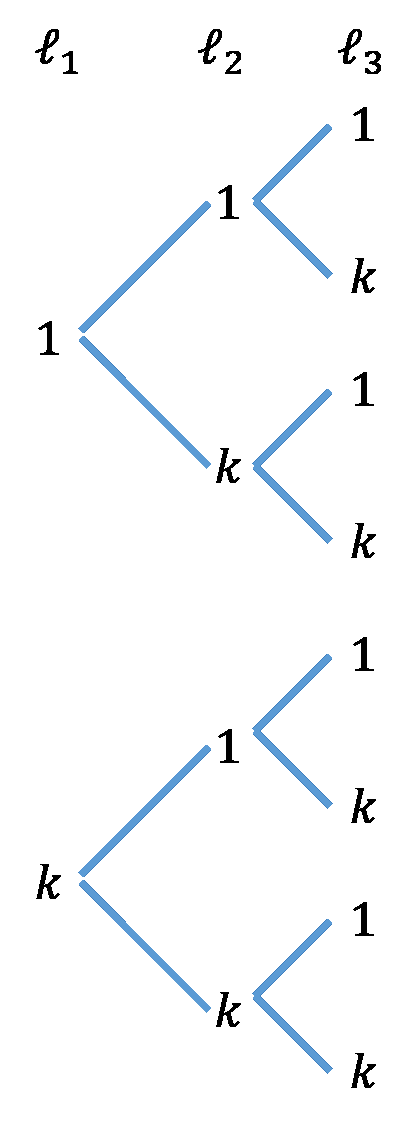
\includegraphics[width=0.95647in,height=2.74852in]{generalBernstein}
	\caption{Diagrama de \'arbol que muestra c\'omo se van agregando la condici\'on de periodicidad a las variables aleatorias para la c\'opula de Bernstein multivariada. Aqu\'i se muestra el caso para 3 variables aleatorias peri\'odicas. N\'otese que tambi\'en muestra la cantidad de sumandos de los elementos de las esquinas, que para este caso es \(2^{3}\).}
	\label{f:treeDiagPer}
\end{figure}



	\chapter{Metodolog\'ia de simulaci\'on de redes de fracturas discretas}
\label{s:dfnModeling}

En este cap\'itulo se muestra de manera esquem\'atica los ingredientes principales de los cap\'itulos anteriores. Para ello, es necesario explicar la manera en que se desarrollar\'an tales ideas principales.

Un diagrama de flujo (flowchart) es una representaci\'on gr\'afica que resalta los elementos de un programa computacional o una metodolog\'ia, las relaciones entre ellos, as\'i como su correspondiente orden de ejecuci\'on (flujo l\'ogico). Para mayor informaci\'on sobre diagramas de flujo su puede consultar los libros de \cite{venit_prelude_2014} y \cite{farrell_programming_2014}.

\begin{table}[H]
	\centering
	\caption{S\'imbolos b\'asicos para construir diagramas de flujo.}
	\label{tab:flowcharCheatsheet}
	\begin{tabular}{|ccl|}
		\hline
		S\'imbolo & Nombre & Descripci\'on \\ \hline
		\tikz \draw (0,0) rectangle (1.5,0.5); & Proceso  & Representa cualquier proceso, c\'alculo \'o funci\'on. \\ \hline
		\tikz \draw (0,0) node[trapezium, trapezium left angle=70, trapezium right angle=110, draw, minimum height=0.5cm] {}; & Input/output & Argumento de entrada o salida. \\ \hline
		\tikz \draw (0,0) node[shape aspect=2,diamond,draw] {}; & Decisi\'on & Representa una decisi\'on binaria, usualmente S\'i o No. \\ \hline
		\tikz \draw (0,0) -- (1,0); & Flecha & Indica la direcci\'on de flujo de control. \\ \hline
	\end{tabular}
\end{table}

Adem\'as, algunos s\'imbolos de la \autoref{tab:flowcharCheatsheet} rellenos con color verde (\tikz \fill[green!30] (0,0) rectangle (0.8,0.3);) representan los inicios de cada diagrama de flujo, mientras que en color rojo (\tikz \fill[red!30] (0,0) rectangle (0.8,0.3);) los finales de los mismos. En el caso de diagramas verticales, el mismo se lee de arriba hacia abajo.

\section{An\'alisis, modelado y simulaci\'on de variables aleatorias}

El enfoque que se utilizar\'a en esta secci\'on es el convencional en ciencias de la tierra en donde, teniendo datos, se procede a caracterizarlos, es decir, a entender su comportamiento en la mayor medida posible. Posteriormente se puede hacer el modelado teniendo en cuenta el paso anterior y posteriormente pueden hacer simulaciones estad\'isticamente equivalentes con los datos. Estos pasos, para el caso univariado, se puede ver reflejado en el diagrama de flujo de la \autoref{f:workflowSim1D}, yendo de lo rojo hacia lo verde.

La caracterizaci\'on se basa principalmente en an\'alisis exploratorio de los datos $x_s$ (en el globo rojo en la \autoref{f:workflowSim1D}). En esta etapa del an\'alisis estad\'istico se analizan individualmente cada una de las propiedades de las fracturas, as\'i como de la red de fracturas. El resultado esperado para esta etapa es entender el fen\'omeno subyacente a los datos, para as\'i poder modelar o sugerir modelos de distribuci\'on de probabilidad para cada una de las propiedades de fractura.

Para lograr este objetivo se hace uso de estad\'igrafos y de gr\'aficas. Por ejemplo, la media proporciona una medida de tendencia centra, mientras que la desviaci\'on est\'andar proporciona informaci\'on sobre qu\'e tan dispersos se encuentran los datos con respecto a la media obtenida. Esto es v\'alido tanto para las longitudes como para las orientaciones, claro, cada variable con su teor\'ia correspondiente. El an\'alisis exploratorio siempre debe de combinar los estad\'igrafos y los gr\'aficos. Para las longitudes se puede utilizar los gr\'aficos de caja y los histogramas principalmente. Para las orientaciones es \'util utilizar las rosetas de orientaciones, pero un histograma resalta m\'as cualquier moda sutil que se escape a la vista en una roseta.

\begin{figure}[H]
	\centering
	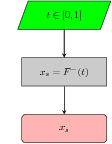
\includegraphics{rvSim}
	\caption{Diagrama de flujo para obtener una simulaci\'on de una variable aleatoria. En este caso puede ser la orientaci\'on o la longitud. Comp\'arese con la \autoref{f:cdf1D}.}
\label{f:workflowSim1D}
\end{figure}

En la siguiente etapa, en color gris en la \autoref{f:workflowSim1D}, se procede a modelar la funci\'on de probabilidad para los datos. Aqu\'i se puede proceder con el enfoque com\'un de hacer pruebas de hip\'otesis para varios modelos propuestos o se puede hacer con el enfoque de los cuantiles de Bernstein-Kantorovich utilizado en este trabajo doctoral.

Para hacer la simulaci\'on, hay que recorrer la \autoref{f:workflowSim1D} en sentido contrario en el que lo hicimos para la caracterizaci\'on y el modelado. Ahora, el algoritmo de simulaci\'on muestra que debemos empezar con un valor simulado $t$ obtenido de una distribuci\'on $Uniforme(0,1)$. La funci\'on cuantil $F^-(t)$ nos proporcionar\'a un valor simulado. De esta manera podemos obtener las simulaciones necesarias para estimar la incertidumbre.

\section{An\'alisis, modelado y simulaci\'on de la estructura de dependencia entre variables aleatorias}

Igual de importante que estudiar individualmente las propiedades de fractura es estudiar la relaci\'on que existen entre tales propiedades. Se recomienda estudiar, primero, las relaciones por pares, es decir de manera bivariada. Dos ejemplos de relaciones bivariadas ser\'ian (1) longitud y apertura, y (2) orientaci\'on y longitud. Posteriormente se puede estudiar de manera trivariada o multivariada pero en estos casos es dif\'icil obtener una idea visual de la estructura de dependencia.

El gr\'afico m\'as \'util para estudiar las dependencias entre variables aleatorias es el gr\'afico o diagrama de pseudo-observaciones. Dicho gr\'afico se forma con las pseudo-observaciones obtenidas a partir de la funci\'on de distribuci\'on emp\'irica (\autoref{e:empF}). Para obtenerlas se presenta el diagrama de flujo en la \autoref{f:pseudoObsWF}. N\'otese que en el diagrama se muestra la funci\'on de distribuci\'on de probabilidad $F(\cdot)$ de manera general, pero en este trabajo se utiliza $F(x)=\hat{F}_n(x)$. Los puntos de cada pseudo-observaci\'on $(u_i, v_i)$, $i \in \{1, \ldots, n\}$ formados con las variables $X$ y $Y$ se grafican en el plano $uv$ (\autoref{fig:pseudoObsPlotGeneration}) para obtener un diagrama de dispersi\'on de las pseudo-observaciones.

\begin{figure}
	\centering
	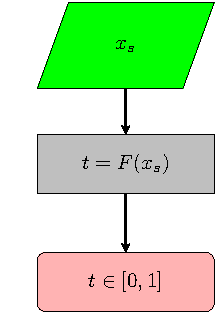
\includegraphics{rvModeling}
	\caption{Diagrama de flujo para obtener las pseudo-observaciones. Comp\'arese con la \autoref{f:cdf1D}.}
\label{f:pseudoObsWF}
\end{figure}


\begin{figure}
	\centering
	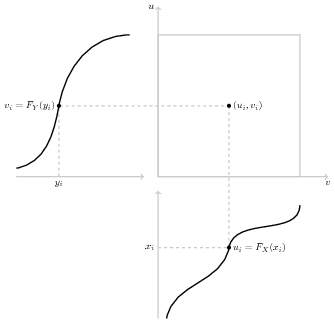
\includegraphics{pseudoObsPlotGeneration}
	\caption{Obtenci\'on del diagrama de pseudo-observaciones con el cual se estudia la dependencia entre dos variables aleatorias. Las funciones de distribuci\'on marginales que se muestran son continuas pero pueden ser no-continuas o una combinaci\'on de ambas.}
	\label{fig:pseudoObsPlotGeneration}
\end{figure}

Dentro del contexto de la teor\'ia de c\'opulas el comportamiento conjunto queda totalmente determinado por la c\'opula, y de manera casi directa por las pseudo-observaciones. Una manera de facilitar el an\'alisis del gr\'afico de pseudo-observaciones es agregando una sub-capa tipo mosaico o pixeles. Un ejemplo muy sencillo se muestra en el recuadro derecho de la \autoref{f:dependenceAnalysis1}. Se propone, como primer paso, que la sub-capa sea determinada por los cuartiles y los valores m\'aximos y m\'inimos de los datos. En particular se propone que los cuartiles se calculen a partir de los modelos de los datos ya que de esta manera se pueden comparar diversas simulaciones sobre un mismo mosaico. En el ejemplo de la \autoref{f:dependenceAnalysis1} se tiene que $q_{1X} = F_X^-(0.25)$, $M=F_Y^-(0.5)$.

\begin{figure}[H]
	\centering
	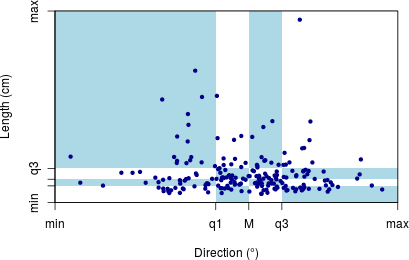
\includegraphics[width=0.4\textwidth]{bivariateInd-15}
	\qquad
	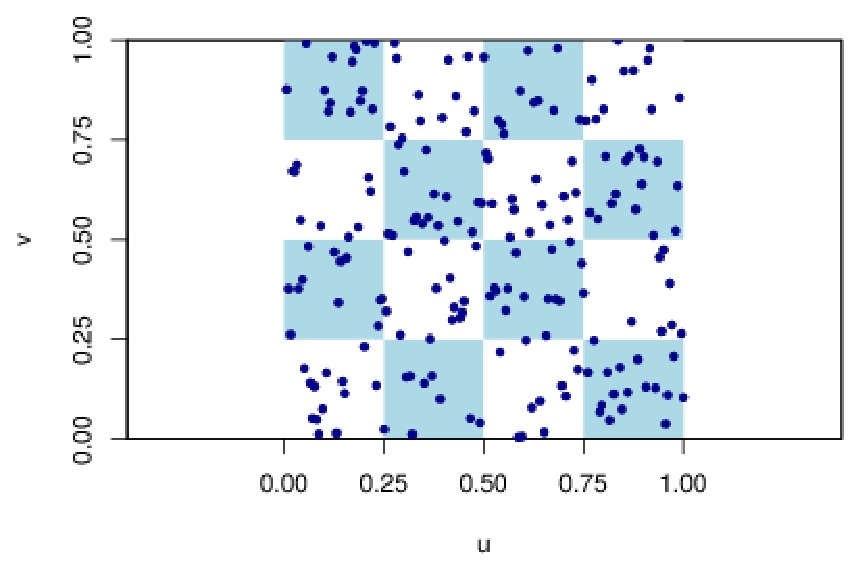
\includegraphics[width=0.4\textwidth]{bivariateInd-14}
	\caption{Diagrama de dispersi\'on con m\'ultiples zonas remarcadas a fin de hacer un an\'alisis exploratorio preliminar.}
	\label{f:dependenceAnalysis2}
\end{figure}

Aunque la c\'opula tiene la informaci\'on de la estructura de dependencia, conviene graficar tambi\'en el diagrama de dispersi\'on de los datos ya que ellos, a diferencia de las pseudo-observaciones, est\'an en el rango real. N\'otese que los cuadros del gr\'afico de pseudo-observaciones se extienden o encogen en el diagrama de dispersi\'on, incluso de forma diferente dependiendo el mosaico/pixel (intervalo bidimensional). En la \autoref{f:dependenceAnalysis2} se muestra otro mosaico para otro conjunto de datos debido a que se quiere resaltar que la estructura de dependencia general se puede descomponer en dos estructuras m\'as simples.

\begin{figure}[H]
	\centering
	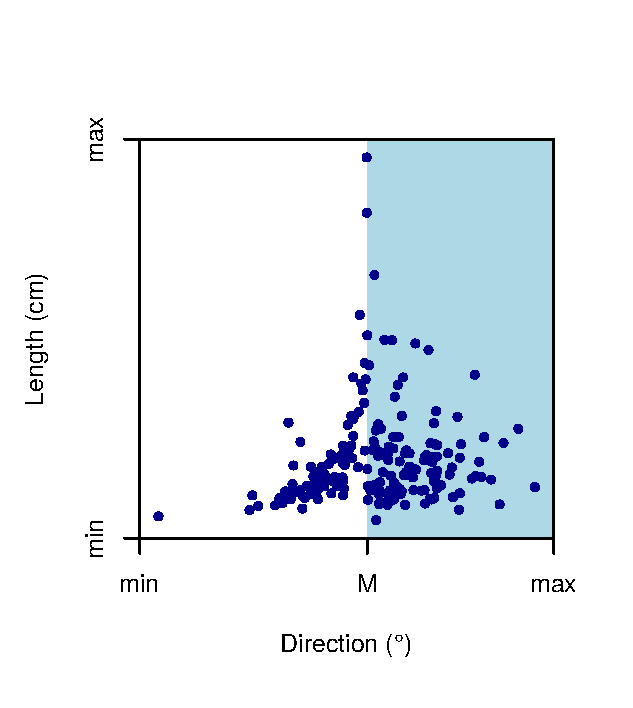
\includegraphics[width=0.4\textwidth]{bivariateDep-24}
	\qquad
	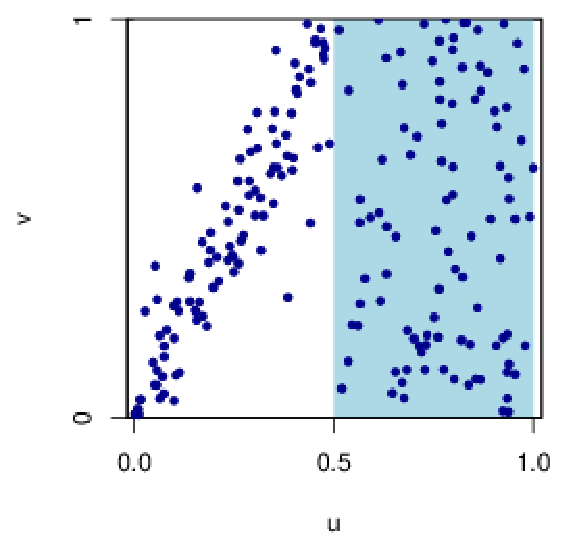
\includegraphics[width=0.4\textwidth]{bivariateDep-26}
	\caption{Diagrama de dispersi\'on en el cual se han resaltado dos zonas con dependencias m\'as simples.}
	\label{f:dependenceAnalysis1}
\end{figure}

% AED: quantitative
De manera cuantitativa, se pueden estimar coeficientes de correlaci\'on y/o hacer pruebas de hip\'otesis sobre la independencia de los datos. Tambi\'en es \'util agregar estos valores al gr\'afico combinado (de dispersi\'on y pseudo-observaciones) ya sea en el gr\'afico o en el pie de figura.

Para la modelaci\'on de la c\'opula bivariada, dentro del contexto de las c\'opulas de Bernstein, se procede a un diagrama de flujo similar al de la \autoref{f:workflowSim1D}. Se analizan los pares de pseudo-observaciones obtenidas mediante la \autoref{f:pseudoObsWF}. \'Estas son inspeccionadas visualmente en un diagrama de dispersi\'on, y cuantitativamente con estad\'igrafos (coeficientes de correlaci\'on \'o asociaci\'on) para determinar si existe o no alguna estructura de dependencia que se deba tomar en cuenta. Si hay dependencia, entonces se modela la c\'opula emp\'irica $\hat{C}_n$ con la cual se ajusta la c\'opula estimada $C$.

\begin{figure}
	\centering
	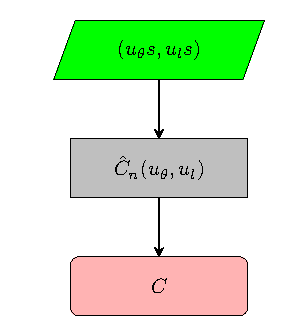
\includegraphics{cop2Dmodeling}
	\caption{Modelaci\'on de la c\'opula a partir de las pseudo-observaciones.}
	\label{f:cop2Dmodeling}
\end{figure}

\section{Diagrama de flujo para el an\'alisis, modelado y simulaci\'on de redes de fracturas discretas tomando en cuenta su estructura de dependencia}

Resulta ilustrativo el diagrama de flujo  de la \autoref{f:rvSim2D} en la modelaci\'on del vector aleatorio bivariado que representa las propiedades de los objetos booleanos en el cual se parte a partir de los datos observados $\theta_i$ y $l_i$. Se han escogido estos s\'imbolos para hacer la analog\'ia con la orientaci\'on y la longitud de fracturas, pero el diagrama de flujo es v\'alido para cualquier par de variables aleatorias continuas.

\begin{figure}[H]
	\centering
	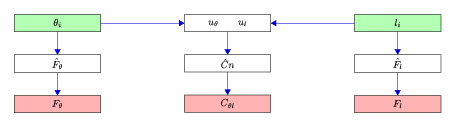
\includegraphics{rvSim2D}
	\caption{Modelaci\'on bivariada de propiedades de objetos booleanos.}
	\label{f:rvSim2D}
\end{figure}

N\'otese que, de arriba hacia abajo, se procede con la caracterizaci\'on de los datos hasta llegar al modelo, en lo parte inferior, tanto de manera univariada como bivariada. En la parte univariada en los extremos izquierdo y derecho del diagrama son los casos particulares del inverso de la metodolog\'ia en la \autoref{f:workflowSim1D}. Si el diagrama en cuesti\'on se recorre en sentido contrario a las l\'ineas de flujo, entonces se obtiene el algoritmo de simulaci\'on bivariado.

\begin{figure}[H]
\begin{center}
\begin{tikzpicture}[scale=1, transform shape]
	\node[trapezium, trapezium left angle=70, trapezium right angle=110,draw, fill=green!30] (n1) at (0,0) {$\mathbf{X}:=\emptyset$};
	\node[draw,below of=n1] (n2) {$n \sim Poisson(\theta |A|)$};
	\node[draw,below of=n2] (n3) {$\forall i \in \{1,\ldots,n\}, \quad \mathbf{x}_i \sim Uniforme(A)$};
	\node[trapezium, trapezium left angle=70, trapezium right angle=110,draw, fill=red!30, below of=n3] (n4) {$\mathbf{X}$};
	\draw (n1)--(n2);
	\draw (n2)--(n3);
	\draw (n3)--(n4);
\end{tikzpicture}
\end{center}
\caption{Diagrama de flujo para obtener ubicaciones espaciales a trav\'es de un proceso puntual. Desde el punto de vista computacional,  la parte superior del diagrama indica crear un arreglo vac\'io que almacene las coordenadas de todos los vertores $\mathbf{x}_i$.}
\label{fig:ppWF}
\end{figure}

Estos dos \'ultimos diagramas de flujo forman la esencia del algoritmo de simulaci\'on de redes de fracturas. Con el algoritmo de la \autoref{f:rvSim2D} se generan los objetos, es decir la orientaci\'on, longitud, etc. de las fracturas; mientras que con el diagrama de la \autoref{fig:ppWF} se obtienen sus ubicaciones espaciales.

El flujo de trabajo est\'andar (\autoref{f:dfnWorkflow}) puede ser siendo utilizado en la parte que corresponde al cluster an\'alisis para determinar familias, el tama\~no de las familias, la direcci\'on y su dispersi\'on, ya que este an\'alisis proporciona informaci\'on valiosa para el entendimiento del sistema geol\'ogico, sin embargo, la modelaci\'on resulta m\'as compatible con los datos si se hace de manera total, ya que no se crean los artificios generados al segmentar bruscamente las familias mediante un valor de corte. Adem\'as, entre mayor sea la cantidad de datos, mejor es la modelaci\'on de funciones de probabilidad.

Con respecto a las caracter\'isticas multivariadas en color azul, es claro que s\'i hay que hacer un an\'alisis basado en la teor\'ia de c\'opulas a como se mostr\'o en la secci\'on pasada. Ya que el enfoque individualista no puede producir relaciones de dependencia que se pueden observar en los sistemas de fracturas reales. \'Este es el aporte principal al conocimiento que se hace con este trabajo de investigaci\'on, en particular la posibilidad para modelar datos orientados y otras propiedades como longitud o apertura.

\begin{figure}[H]
	\centering
	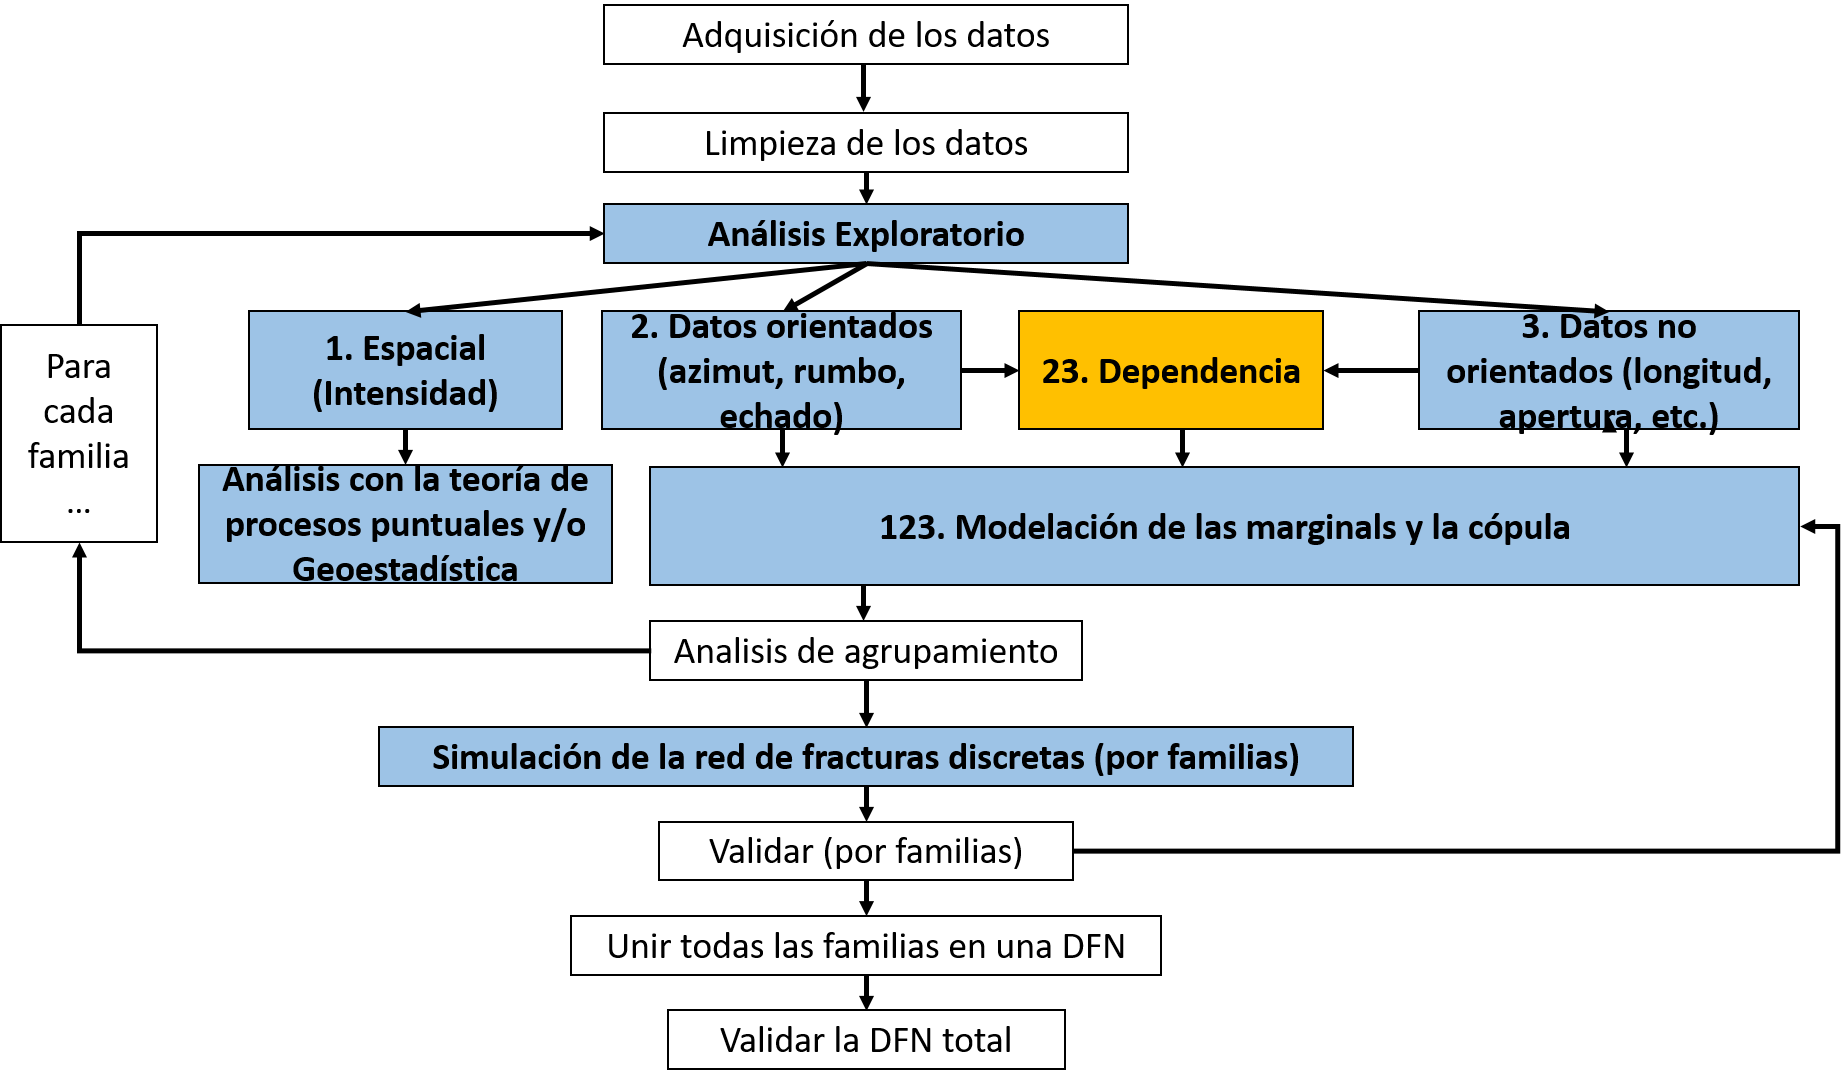
\includegraphics[width=0.8\textwidth]{workflow}
\caption{Flujo de trabajo para la caracterizaci\'on, modelado y simulaci\'on de redes de fracturas discretas en medios porosos fracturados.}
	\label{f:dfnWorkflow}
\end{figure}

El flujo de trabajo (\autoref{f:dfnWorkflow}) comienza en la parte superior con la adquisici\'on de los datos, posteriormente hay que limpiarlos para poder hacer un an\'alisis exploratorio, el cual se realiza de manera univariada (intensidad, orientaci\'on, longitud, apertura, ...) y de manera bivariada se estudian las propiedades mediante las pseudo-observaciones. Como resultado hasta este momento se pudo haber identificado grupos/clusters, los cuales se pueden separar para comenzar el ciclo desde al an\'alisis exploratorio para cada uno de los grupos. Posteriormente se ajustan modelos a cada una de las variables y de manera conjunta con c\'opulas. Estos modelos permiten las simulaciones de fracturas por familias, las cuales tienen que ser validadas, nuevamente, mediante otro an\'alisis exploratorio para verificar que cumple con las mismas propiedades estad\'isticas que los datos. Ahora ya se pueden integrar todas las familias y para finalmente validar la familia global.

Cabe mencionar que el an\'alisis de dependencia tambi\'en puede ayudar para clasificar familias que se distingan de manera bivariada una de otra. Es decir, tambi\'en se puede integrar el an\'alisis de dependencia a cada una de las familias obtenida con el an\'alisis de clusters.


	\chapter{Casos de estudio}
\label{ch7:examples}

A continuaci\'on, se aplican los resultados de los cap\'itulos anteriores a dos casos particulares.
El primer caso fue tomado del art\'iculo de \citet{mendoza-torres_bernstein_2017}. 
En \'el se muestra la aplicaci\'on a una red de fracturas considerando solamente la dependencia entre la orientaci\'on y la longitud.
La aplicaci\'on trivariada (orientaci\'on-longitud-apertura) se muestra en el segundo caso.

\section{Caso bivariado orientaci\'on-longitud}

\subsection{Descripci\'on de los datos}
\label{ss:synthData}

Aunque la metodolog\'ia es v\'alida para cualquier sistema de fracturas, en esta secci\'on se presenta una red de fracturas cuyo comportamiento es frecuentemente encontrado dentro de la corteza terrestre. Debido a la falta de datos reales, se gener\'o un conjunto de datos tratando de reproducir cierto conocimiento geol\'ogico:

% Extension fracture
\setlength{\epigraphwidth}{0.9\textwidth}
\epigraph{\textit{Fracura de extensi\'on}: Fractura formada por la extensi\'on perpendicular a las paredes de la fractura. La magnitud de la extensi\'on puede ser min\'uscula como en el caso de 
\textit{juntas}, o puede ser tan grande como las \textit{venas}}{\citet[p. 434]{fossen_structural_2010}}

\setlength{\epigraphwidth}{0.9\textwidth}
\epigraph{las juntas de cizalla comunmente ocurren en \textit{conjuntos conjugados}\ldots las juntas de cizalla ocurren en conjuntos conjugados oblicuos en donde las juntas de extensi\'on aparecen como juntas longitudinales y transversas que un par ortogonal}{\citet[p. 17]{singhal_applied_2010}}
%singhal_applied_2010 "Shear joints ... forming an orthogonal pair (Fig. 2.7)."

A\'un m\'as, algunos sistemas de fracturas tienen relaciones espec\'ificas de orientaci\'on y longitud:

\setlength{\epigraphwidth}{0.9\textwidth}
\epigraph{Los mineros se refieren a estas fracturas en direcciones caracter\'isticas como \textit{cruceros de carb\'on}: un crucero constituido por por face cleats, largas fracturas dominantes (juntas sistem\'aticas) que pueden extenderse por varios metros de manera horizontal; y por, butt cleats, otro conjunto de fracturas m\'as cortas escasamente desarrolladas que terminan en las face cleats en \'angulos rectos (juntas transversales).}{\citet{davis_structural_2011}}
%2012-Structural geology of rocks and regions (Davis, Raynolds and Kluth), page 241: "Miners refer to these two distinctive fracture directions as coal cleats: a face cleat composed of long continuous dominant fractures (systematic joints) that extend for many meters horizontally; and a butt cleat composed of shorter, somewhat more poorly developed fractures that terminate at right angles against the face cleat (cross joints)... “Scatter” in the orientations of the face cleats is related primarily to the influence of local stresses, which can cause shifts of joint trends from the direction(s) predicted by the regional orientation of far-field stresses, and which at a much finer scale can cause shifts in orientations of parts of individual joint surfaces." "Jointing Associated with Large Individual Folds" "It is not uncommon for faults to occur in conjugate sets (Figure 6.66A) that intersect in an acute angle, commonly 60"
%1998 Laubach, Marrett, Olson, Scott Characteristics and origins of coal cleat. "cleat lengths and heights are reported to range from microns to meters. Tremain et al., 1991.Yet these cleats are arranged in a hierarchy of sizes that includes fractures of decimeter size 'master cleats', Fig. 1."

% Rose diagrams of coal cleats:
%2004_Gillam, Flottmann and Hillis_Natural fracture characterisation in a coal measure succession. an analogue for coal seam methane and tight gas reservoirs
%2006 the nature of naturally fractured reservoir schlumberger
%2008_ Pashin, Jin, Zheng_2Discrete Fracture Network Models for Risk Assessment of Carbon Sequestration in Coal

%Usually, fractures form as conjugate sets \cite{}[section 2.2.3.5, and fig. 2.9] 2010-Applied Hydrogeology of Fractured Rocks (Singhal and Gupta)."the observed length of fracture trace depends on the relative orientation between the fracture plane and the exposure face"

Para mayor detalle y datos en los que se basa esta afirmaci\'on sobre los cruceros de carb\'on cons\'ultese los art\'iculos de \citet{rodrigues_coal_2014}; \citet{laubach_characteristics_1998}; y \citet{datta_coal_2016}. 

A partir de este conocimiento de la geolog\'ia estructural, el conjunto de datos de orientaci\'on y longitud a estudiar debe satisfacer:

\begin{itemize}
	\item Tener dos familias $f90$ y $f0$, siendo esta \'ultima la familia dominante, es decir, con fracturas m\'as largas.
	%	see FIGURE 5 of http://www.cdc.gov/niosh/mining/userfiles/works/pdfs/ri7910.pdf
	\item las longitudes de la familia $f90$ son menores que la familia conjugada.
	\item La familia en la direcci\'on Este ($f90$), con fracturas m\'as peque\~nas, debe tener m\'as fracturas que la familia dominante.
	%	\item length distribution is bimodal? No always, look for references.
	%"Renshaw, 1999, Conectivity..."
	%1997 Clemo, Smith _ A hierarchical model for solute transport in fractured media
	%	\item f0 is more disperse than f90? look for references
\end{itemize}

Nos referiremos al conjunto de datos a estudiar como \textit{los datos}, o los \textit{datos sint\'eticos}, y ser\'an considerados como si fueran reales. Estos 400 datos se componen de las coordinadas cartesianas de los centros de fracturas $\vec{x} = (x,y) \in [0,400] \times [0,400]$.
Debido a razones de visualizaci\'on y comparaci\'on, estos centros de fracturas se obtuvieron con un proceso homog\'eneo de Poisson con intensidad $\theta = 1$.
Las direcciones de rumbo de las fracturas fueron muestreadas de una combinaci\'on de dos distribuciones de von Mises con par\'ametros mostrados en la \autoref{t:movMpar}.
Estos \'angulos se encuentran en el rango $[0, 180)$ en un sistema de coordenadas geogr\'afico (Norte = 0$^{\circ}$, Este = 90$^{\circ}$).
Las longitudes fueron muestreadas mediante una distribuci\'on lognormal.
Aunque generalmente las fracturas muestran un comportamiento auto-af\'in por lo que se observan de manera similar a varias escalas; atendiendo a las citas geol\'ogica de \citet{davis_structural_2011} en este trabajo, utilizaremos cm para las longitudes de fracturas.

Con respecto a la estructura de dependencia, los datos anteriores se muestrearon pegando dos c\'opulas (gluing copulas) de Placket (\verb|copBasic::PLACKETTcop|). Para pseudo-observaciones en el intervalo $u_{\theta} = [0, 0,5)$, se utiliz\'o una dependencia aproximadamente lineal y directa (par\'ametro de placket = $0.06$); para las pseudo-observaciones en el intervalo $u_{\theta} = [0.5, 1]$ se utiliz\'o una dependencia aproximadamente lineal e inversa (par\'ametro de placket = $20$). Esta estructura de dependencia se puede observar en la \autoref{f:scatterplot}.

Como resultado, la red de fracturas discretas en ser analizadas y modelada con la metodolog\'ia est\'andar y conjunta se muestra en la \autoref{f:dfn}. En esta figura, para analizar la relaci\'on de dependencia entre direcci\'on y longitud, se colorearon en negro las fracturas con longitudes mayores a 51 cm mientras que las fracturas menores en azul claro. Este corte se bas\'o en el 90$^\circ$ percentil del modelo de longitudes. Es decir, aproximadamente el 10\% del total de fracturas son negras.

\begin{figure} % Parameters meaning: https://www.sharelatex.com/learn/Positioning_images_and_tables#Positioning_tables
	\centering
	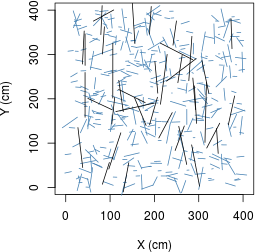
\includegraphics{fig2}
	\caption{Representaci\'on gr\'afica de la red de fracturas de los datos sint\'eticos. Aproximadamente el 10\% de las fracturas son de color negro.}
	\label{f:dfn}
\end{figure}

Las orientaciones fueron generadas usando la funci\'on \verb|rmixedvonmises| del paquete \verb|circular| \citep{agostinelli_r_2013} con los par\'ametros de la \autoref{t:movMpar}. En la \autoref{t:circStats} se muestran algunos de sus estad\'igrafos, calculados con el mismo paquete.
La media circular (89.7$^{\circ}$) es muy similar a la mediana
(88.5$^{\circ}$). Ambos estad\'igrafos muy parecidos a la familia f90. El valor muy peque\~no de asimetr\'ia es un indicador de que la distribuci\'on es altamente sim\'etrica. Estos resultados tambi\'en se pueden visualizar en la \autoref{f:rose}, la cual muestra que la familia f90 tiene una poblaci\'on mayor que la familia en la direcci\'on N-S. \'Esta \'ultima observaci\'on en total acuerdo con los requerimientos del modelo.

\begin{table}[H]
	\centering
	\begin{tabular}{ |c|c|c|c|}
		\hline
		familia & proporci\'on & $\mu (^{\circ}$) & $\kappa$ \\ \hline
		f0     &    0.3     &   0   & 10       \\ \hline
		f90    &    0.7     &  90   & 10       \\ \hline
	\end{tabular}
	\caption{Par\'ametros de la combinaci\'on de dos distribuciones de von Mises de donde fueron muestreadas las 400 direcciones de la red de fractura a modelar.}
	\label{t:movMpar} % stands for "Table" of 'm'ixture 'o'f two 'v'on 'M'ises distributiions 'par'ameters
\end{table}


\begin{figure}[H]
	\centering
	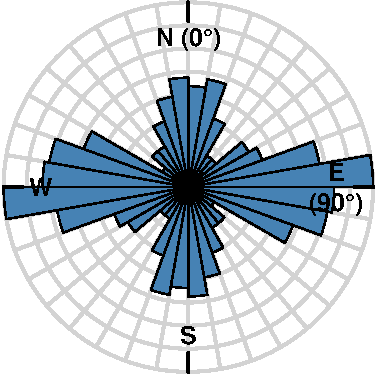
\includegraphics{fig3}
	\caption{Roseta de los datos a analizar. f0 est\'a en la direcci\'on N-S, f90 en la direcci\'on perpendicular (E-O).}
	\label{f:rose}
\end{figure}

\begin{table}[H]
	\centering
	\begin{tabular}{ |c|c|}
		\hline
		Estad\'igrafo         &  valor   \\ \hline\hline
		Mediana             & 88.458$^{\circ}$ \\ \hline
		$\mu$              & 89.728$^{\circ}$ \\ \hline
%		Longitud resultante   &  0.306   \\ \hline
		Desviaci\'on est\'andar &  44.063  \\ \hline
		Asimetr\'ia           &  0.045   \\ \hline
	\end{tabular}
	\caption{Estad\'istica circular de las direcciones de los datos sint\'eticos.}
	\label{t:circStats}
\end{table}



Las longitudes fueron generadas utilizando lo funci\'on \verb|rlnorm| del paquete \verb|stats|. Los par\'ametros de la distribuci\'on lognormal en dicha funci\'on son $meanlog = 3$, $sdlog= 0.73$, la media y la desviaci\'on est\'andar en la escala logar\'itmica. Los estad\'igrafos en la \autoref{t:lengthStats} muestran la diferencia entre los valores de la media y la mediana. Esto es una muestra de alta asimetr\'ia tambi\'en en la misma tabla. El histograma adem\'as muestra una peque\~na moda alrededor de los 70 cm.

\begin{figure}
	\centering
	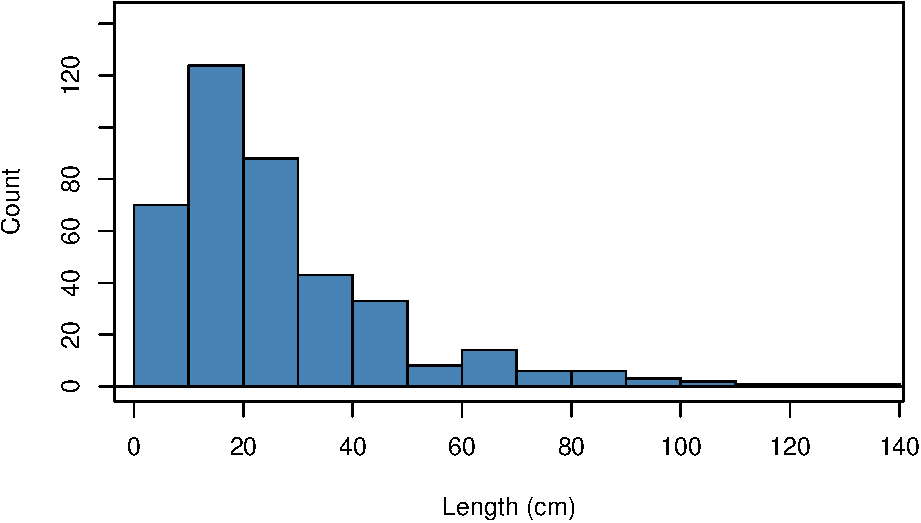
\includegraphics[width=0.8\textwidth]{fig4}
	\caption{Histograma de las longitudes de fractura. La longitud se distribuye lognorm(meanlog = 3.00, sdlog = 0.73)}
	\label{f:hist}
\end{figure}

\begin{table}[H]
	\centering
	\begin{tabular}{ |c|c|}
		\hline
		Estad\'igrafo         & valor  \\ \hline\hline
		Mediana             & 20.389 cm \\ \hline
		Media               & 26.186 cm \\ \hline
		Desviaci\'on est\'andar & 20.894 cm \\ \hline
		Asimetr\'ia           & 1.914  \\ \hline
	\end{tabular}
	\caption{Estad\'igrafos de las longitudes de los datos sint\'eticos.}
	\label{t:lengthStats}
\end{table}



La \autoref{f:cdfDL} muestra las funciones de distribuci\'on acumulativa de la direcci\'on y de la longitud. Aunque estos datos tienen un comportamiento marcadamente diferente, la funci\'on cuantil de Bernstein-Kantorovich muestra representar bastante bien ambos comportamientos. Para los datos orientados, en este trabajo se prefiere la flexibilidad de dicha funci\'on cuantil en vez de 'ajustar artificialmente una funci\'on como la von Mises.

\begin{figure}
	\centering
	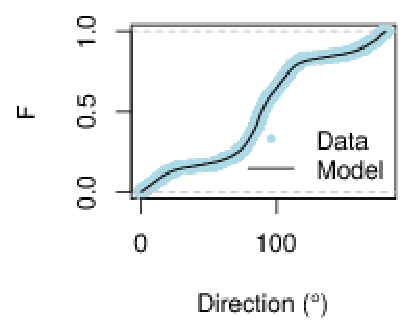
\includegraphics{fig5left}
	\qquad
	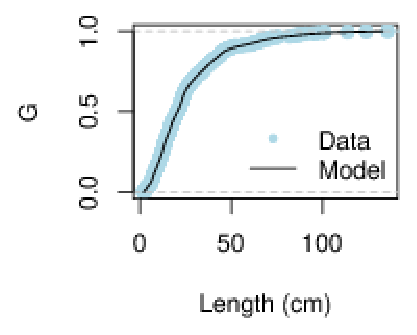
\includegraphics{fig5right}
	\caption{Funci\'on de distribuci\'on acumulativa y su respectivo modelo ajustado mediante la funci\'on cuantil de Bernstein-Kantorovich. Izquierda: direcci\'on; Derecha: longitud.}
	\label{f:cdfDL}
\end{figure}

El diagrama de dispersi\'on (\autoref{f:scatterplot}) direcci\'on-longitud y su correspondiente gr\'afico de pseudo-observaciones $uv$ se muestran para entender el comportamiento bivariado, es decir, para entender la estructura de dependencia subyacente. La diferencia entre ambos gr\'aficos reside en que el diagrama de dispersi\'on de los datos vive en el producto cartesiano de los rangos de las dos variables aleatorias mientras que el gr\'afico de pseudo-observaciones vive en el cuadrado unitario ($[0, 1] \times [0, 1]$).

Dado que el an\'alisis de dependencia utilizando la teor\'ia de c\'opula no es est\'andar fuera del \'ambito estad\'istico, expliquemos brevemente c\'omo se efect\'ua. Los valores en los ejes del gr\'afico de pseudo-observaciones \autoref{f:scatterplot} corresponden a las probabilidades (acumulativas) de los cuantiles (ejes en el diagrama de dispersi\'on). Por ejemplo, en el eje horizontal del diagrama de dispersi\'on (izquierda de \autoref{f:scatterplot}), el \'angulo 90$^\circ$ (la media) corresponde a $u = 0.5$ en el gr\'afico de pseudo-observaciones; mientras que el tercer cuantil en el diagrama de dispersi\'on corresponde a $u = 0.75$. El \'angulo 0$^\circ$ corresponde a $u=0$. De manera similar para el eje vertical.

El gr\'afico de pseudo-observaciones permite entender de manera visual la estructura de dependencia. De esta manera se puede estudiar el efecto que tiene la estructura de dependencia sobre el diagrama de dispersi\'on.

El coeficiente de correlaci\'on de rango para estos datos ($\rho_M = 0.635$) es un indicador de que la orientaci\'on no es independiente de la longitud. Este n\'umero fue calculado con los c\'odigos que se pueden encontrar en el trabajo de \citet{tu_study_2015}.

Un indicador m\'as confiable para determinar independencia se debe basar en la teor\'ia de c\'opulas. La funci\'on \verb|indepTest|  del paquete \verb|copula| permite hacer una prueba de independencia basada en c\'opulas. Para los datos en uso se obtuvo un estad\'istico de la prueba con valor 0.408 y un p-valor de 5\e{-4}, lo que indica que la independencia es rechazada. Por lo tanto, s\'i es \'util continuar con el modelado de la estructura de dependencia.

%The correlation coefficient were computed with the \verb|hoefCOP| function from the \verb|copBasic| package \citep{Asquith2015} and the codes provided in \citet{tu_study_2015}.

\begin{figure}[H]
	\centering
	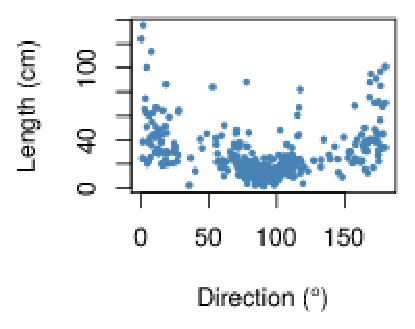
\includegraphics{fig6left}
	\qquad
	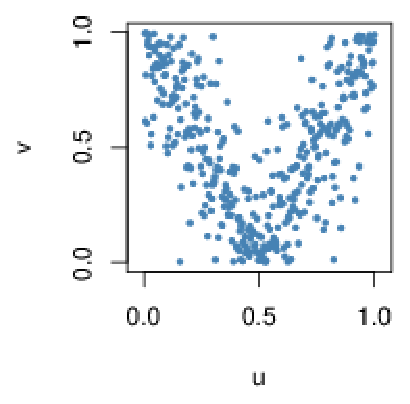
\includegraphics{fig6right}
	\caption{Diagrama de dispersi\'on de la longitud vs direcci\'on (izquierda), y su correspondiente gr\'afico de pseudo-observaciones (derecha).}
	\label{f:scatterplot}
\end{figure}

En el diagrama de dispersi\'on claramente se muestra una moda en la direcci\'on N-S pero la otra familia es casi indistinguible. Es decir, la familia f0 resalta m\'as que la familia f90. En contraste, en la roseta de direcciones sucede lo casi contrario. Ah\'i s\'i se pueden visualizar claramente ambas modas, pero la que m\'as resalta es la de la familia en la direcci\'on E-O. En el diagrama de dispersi\'on se puede observar que la probabilidad de obtener fracturas con longitudes menores a, digamos, 18cm, dentro de la familia N-S es casi cero. Un fen\'omeno inverso se puede observar en la familia E-O: muchas fracturas peque\~nas y casi ninguna grande.

\'Este fen\'omeno se debe a la estructura de dependencia mostrada en el gr\'afico de pseudo-observaciones. N\'otese tambi\'en que hay muchas m\'as fracturas peque\~nas (menores a 51 cm, por ejemplo) que fracturas largas a lo largo del rango de direcciones, $[0, 180^\circ$).

\subsection{La metodolog\'ia est\'andar}

Para el siguiente an\'alisis es conveniente distinguir entre las palabras 'sint\'etico' y simulado. Cuando usemos el primero ser\'a para referirnos al conjunto de datos de la secci\'on pasada. N\'otese pue para un conjunto de datos pueden existir m\'ultiples simulaciones.

En esta secci\'on se muestran resultados utilizando una metodolog\'ia cuasi-est\'andar. El t\'ermino \textit{cuasi} se debe a que no se hace clasificaci\'on de fracturas alguna ya que con la funci\'on cuantil de Bernstein-Kantorovich se puede modelar directamente datos multimodales. De esta manera, las funciones marginales univariadas son modelas de manera id\'entica que en la secci\'on siguiente. Esto nos permite ser m\'as objetivos en la comparaci\'on del an\'alisis bivariado, que en la metodolog\'ia est\'andar se hace simulando cada variable de manera independiente.

Los modelos marginales univariados utilizados ser\'an los mismos que en la \autoref{f:cdfDL}. Para facilitar la comparaci\'on, los anchos de clase son los mismos tanto en la roseta de direcciones de los datos sint\'eticos (\autoref{f:rose}) como en la delos datos simulados (\autoref{f:roseSim}. De manera similar para los histogramas de los datos sint\'etico y los simulados. De manera bivariada, los rangos tanto en el eje vertical como en el horizontal fueron fijados. Tambi\'en en la parte espacial, los centros de las fracturas son exactamente los mismos.

La roseta de las simulaciones independientes (\autoref{f:roseSim}) parece m\'as suavizada, es decir, comparando con la roseta de los datos (\autoref{f:rose}), hay menos contraste entre las modas y los valles. A diferencia de este comentario, las ubicaciones de dichas modas y valles son satisfactoriamente reproducidas. Incluso, una ligera asimetr\'ia alrededor de 90$^\circ$ es reproducida. De manera cuantitativa, los estad\'igrafos circulares (\autoref{t:circStatsSim}) tambi\'en muestra lo bueno que es el ajuste. Sin embargo, el aumento de desviaci\'on est\'andar remarca la sospecha del efecto de suavizado.

%For a comparison to the methodology of this work, \autoref{f:uvSimInd} shows the pseudo-observations of a simulation made with the standard methodology in which no dependendence is modeled. This figure corresponds to exactly the same marginal dataset $\{\theta_i, l_i\}$ as the simulation with dependence in \autoref{f:uvSim}, i. e, the mean, variance and other statistics are identical to those in \autoref{t:circStatsSim} and \autoref{t:lengthStatsSim} but the difference is the underlying copula.

%In \autoref{f:alSimInd} is shown the consequences in the scatterplot and the DFN of having the dependence structure of \autoref{f:uvSimInd}. Again, the 90th percentile (51cm) has been used as a cutoff to highlight the 10\% of the larger fractures. Notice the direction of these in the scatterplot and the DFN are more disperse (no preferred direction) than in the simulation taken into account the dependence structure (\autoref{f:dfnSim}).

\begin{figure}
	\centering
	\includegraphics{fig7}
	\caption{Roseta de orientaciones de una simulaci\'on. Comp\'arese con \autoref{f:rose}}.
	\label{f:roseSim}
\end{figure}

\begin{table}[H]
	\centering
	\begin{tabular}{ |c|c|}
		\hline
		Estad\'igrafo         & valor  \\ \hline\hline
		Mediana             & 83.930$^{\circ}$  \\ \hline
		$\mu$              & 85.431$^{\circ}$ \\ \hline
%		Longitud resultante   & 0.233  \\ \hline
		Desviaci\'on est\'andar & 48.920 \\ \hline
		Asimetr\i'a           & 0.166 \\ \hline
	\end{tabular}
	\caption{Estad\'igrafos circulares de las direcciones de una simulaci\'on de los datos. Comp\'arese con \autoref{t:circStats}.}
	\label{t:circStatsSim}
\end{table}



Las longitudes, simuladas independientemente de las orientaciones, tambi\'en fueron reproducidos. N\'otese por ejemplo que el valle observado a aproximadamente 55cm se reproduce en es histograma (\autoref{f:histSim}). La moda sutil alrededor de los 70 cm tambi\'en aparece en esta simulaci\'on. Por el lado cuantitativo, la media y la mediana son distintos entre s\'i pero muy parecidos sus correspondientes en los datos sint\'eticos. Aqu\'i tambi\'en se muestra un aumento en la desviaci\'on est\'andar.

\begin{figure}
	\centering
	\includegraphics[width=0.8\textwidth]{fig8}
	\caption{Histograma de longitudes de una simulaci\'on. Comp\'arese con la \autoref{f:hist}.}
	\label{f:histSim}
\end{figure}

\begin{table}[H]
	\centering
	\begin{tabular}{ |c|c|}
		\hline
		Estad\'igrafo         & valor  \\ \hline\hline
		Mediana             & 22.877 cm \\ \hline
		Media               & 29.400 cm \\ \hline
		Desviaci\'on est\'andar & 23.930 cm \\ \hline
		Asimetr\i'a           & 1.752  \\ \hline
	\end{tabular}
	\caption{Estad\'igrafos de las longitudes de una simulaci\'on de los datos. Comp\'arese con la \autoref{t:lengthStats}.}
	\label{t:lengthStatsSim}
\end{table}



Esta coherencia entre la simulaci\'on y los datos tambi\'en se observa en la cercan\'ia de la funci\'on de distribuci\'on acumulativa emp\'irica con la de los modelos (\autoref{f:cdfLs}). \'Este es el resultado de la cualidad no-param\'etrica de la funci\'on cuantil de Bernstein-Kantorovich.

\begin{figure}[H]
	\centering
	\includegraphics{fig9left}
	\qquad
	\includegraphics{fig9right}
	\caption{Funciones de distribuci\'on acumulativa emp\'irica de los datos y sus respectivos modelos. Izquierda: Direcciones; Derecha: longitudes.}
	\label{f:cdfLs}
\end{figure}

N\'otese sin embargo que en el caso bivariado (\autoref{f:alSimInd}) el modelado no es tan satisfactorio como en el caso univariado.
Tanto en el diagrama de dispersi\'on como en el gr\'afico de pseudo-observaciones los puntos est\'an m\'as dispersos, sin forma preferencial alguna.
Cuantitativamente, el coeficiente de correlaci\'on es claramente diferente ($\rho_M = 0.016$).
Ni el diagrama de dispersi\'on ni el gr\'afico de pseudo-observaciones muestra la estructura de los datos que se quiso modelar. La raz\'on: la simulaci\'on no tom\'o en cuenta ning\'un dato bivariado. La metodolog\'ia est\'andar siempre produce resultados como \'este gr\'afico de pseudo-observaciones: puntos distribuidos independientemente (\autoref{f:alSimInd}).

\begin{figure}[H]
	\centering
	\includegraphics{fig10left}
	\qquad
	\includegraphics{fig10right}
	\caption{Diagramas de dispersi\'on de la simulaci\'on. Izquierda: los datos; derecha: las pseudo-observaciones.}
	\label{f:alSimInd}
\end{figure}

La DFN resultante paga el precio al mostrar, por ejemplo, que el 10\% de las fracturas m\'as largas no est\'an preferencialmente en la direcci\'on N-S como los datos originales. Al contrario, ahora las fracturas m\'as largas se encuentran en la direcci\'on E-W.

\begin{figure}[H]
	\centering
	\includegraphics{fig11}
	\caption{DFN de una simulaci\'on de los datos. Comp\'arese con \autoref{f:dfn}.}
	\label{f:DFN_simInd}
\end{figure}

\subsection{El enfoque con la c\'opula de Bernstein}

La metodolog\'ia en esta secci\'on s\'i incluye la estructura de dependencia a trav\'es de la c\'opula de Bernstein de las pseudo-observaciones en la \autoref{f:scatterplot}. Con este modelo de c\'opula, se simularon nuevas pseudo-observaciones (izquierda de  la \autoref{f:alSim}) utilizando los pasos 1 y 2 del algoritmo de simulaci\'on bivariado. Despu\'es, utilizando el paso 3, se obtuvieron los valores simulados de orientaci\'on y longitud (derecha de la \autoref{f:alSim}) mediante las funciones cuantiles mostradas en la \autoref{f:cdfDL}.

La teor\'ia de c\'opulas permiti\'o tener las mismas marginales que en el caso independiente, es decir, la roseta de direcciones, el histograma de longitudes y los estad\'igrafos son exactamente los mismos que en el caso independiente. La diferencia radica en la estructura de dependencia. La \autoref{f:alSim} muestra los diagramas de dispersi\'on. N\'otese el contraste en aspecto visual de esta simulaci\'on comparada con los datos reales. Cuantitativamente, el coeficiente de correlaci\'on de rango ($\rho_M = 0.571$) tambi\'en es coherente con el de los datos.

\begin{figure}[H]
	\centering
	\includegraphics{fig12left}
	\qquad
	\includegraphics{fig12right}
	\caption{Diagrama de dispersi\'on y gr\'afico de pseudo-observaciones de la simulaci\'on que toma en cuenta la modelaci\'on de la estructura de dependencia. Comp\'arese con la \autoref{f:scatterplot} y con la \autoref{f:alSimInd}.}
	\label{f:alSim}
\end{figure}

La red de fracturas discretas correspondiente, al igual que en los datos sint\'eticos, muestra la preferencia de las fracturas m\'as largas por la direcci\'on N-S. Sin embargo, sin faltar a la realidad, todav\'ia existe la posibilidad de obtener fracturas en otras direcciones.

\begin{figure}[H]
	\centering
	\includegraphics{fig13}
	\caption{DFN de la simulaci\'on basada en las c\'opulas de Bernstein. Comp\'arese con \autoref{f:dfn} y con \autoref{f:dfnSim}.}
	\label{f:dfnSim}
\end{figure}


	\section{Caso de estudio trivariado:  orientaci\'on-longitud-apertura.}
\label{s:caseStudy3D}

Para mostrar la utilidad de esta teor\'ia se gener\'o computacionalmente un sistema de fracturas (\autoref{f:fracAbs}) al cual se le dio una estructura de dependencia compleja en el que las fracturas en la direcci\'on vertical son m\'as peque\~nas que las que est\'an en direcci\'on horizontal. Adem\'as, la relaci\'on longitud-apertura es mon\'otona, aunque no lineal (\autoref{f:psdObs}). Por otro lado, la ubicaci\'on espacial fue simulada mediante un proceso puntual de Poisson con intensidad constante ya que un proceso de Poisson con intensidad variable no permiti\'o una mejor visualizaci\'on de la red de fracturas. Los par\'ametros de los modelos se muestran a continuaci\'on:

\begin{figure}[H]
\centering
\includegraphics[height=0.4\textwidth,  keepaspectratio = TRUE]{DFN-1}
\caption{Sistema de fracturas a analizar.}
\label{f:fracAbs} % 'frac'ture 'abs'traction = conceptual model
\end{figure}

\begin{itemize}
  \item $x - poisproc(I = 0.5)$
  	\item $\theta - vonmises(\mu = 90, 180; \kappa = 10, 10))$
  \item $L - lnorm(\mu = 4, 2; \sigma = 0.4, 0.6)$
    \item $b - lnorm(\mu = exp(-4); \sigma = exp(1))$
\end{itemize}

N\'otese que tanto los datos de orientaci\'on como los datos de longitud fueron simulados cada uno como una combinaci\'on de las distribuciones de probabilidad correspondientes, lo que resulta en distribuciones bimodales tanto para los \'angulos como para las longitudes. La relaci\'on de dependencia entre estas dos variables (\autoref{f:psdObs}) parece f\'acil ya que es una uni\'on de dependencia lineal y uniforme, sin embargo, en la pr\'actica es dif\'icil modelarla cuando se dan de esta manera.

Por fines de comparaci\'on con simulaciones de este mismo sistema de fracturas, a continuaci\'on, se muestran algunos estad\'igrafos del an\'alisis exploratorio de los datos. Las direcciones de las fracturas est\'an medidas en un rango de 0$^\circ$ a 180$^\circ$ sobre un sistema de coordenadas geogr\'afico. Los estad\'igrafos de la variable direccional $\Theta$ fueron calculados mediante la estad\'istica de datos orientados \citep{mardia_directional_2000,fisher_statistical_1995,jammalamadaka_topics_2001}.

\begin{table}[htpb]
\begin{center}
	\begin{tabular}{|c|c|c|} % r = right aligment, c = centered
		\hline % adds a horizontal line
		\textbf{Estad\'igrafos} & \textbf{$L$} & \textbf{$\theta$} \\
		\hline\hline
		$\mu$    & 34.6203 & 36.3756 \\
		Mediana   & 24.1315 & 36.5734 \\
		$\sigma$ & 30.3200 & 59.5328 \\
		Asimetr\'ia & 0.8456  & -0.2369 \\ \hline
	\end{tabular}
\end{center}
    \caption{Estad\'igrafos de las longitudes y las orientaciones. Los estad\'igrafos de $\theta$ fueron estimados mediante la estad\'istica de datos orientados. Comp\'arese con la \autoref{tab:trivSim}.}
    \label{tab:triv}
\end{table}

N\'otese que estos estad\'igrafos no representan adecuadamente los modelos ya que no son modelos univariados. Sin embargo, se espera que la metodolog\'ia presentada s\'i logre reproducir cada uno de los ingredientes para generar esta red de fracturas, as\'i como los estad\'igrafos.

\begin{figure}
	\centering
	\includegraphics[width=0.8\textwidth,  keepaspectratio = TRUE]{x-1}
	\caption{Matrix de diagramas de dispersi\'on con las correspondientes distributiones marginales en las entradas de la diagonal.}
\end{figure}

\begin{figure}
	\centering
	\includegraphics[height=0.4\textwidth,  keepaspectratio = TRUE]{empCopScatter-1}
	\includegraphics[height=0.4\textwidth,  keepaspectratio = TRUE]{empCopScatter-2}
	\caption{Diagramas de dispersi\'on de las pseudo-observaciones.}
	\label{f:psdObs} % Pseudo observaciones
\end{figure}

Con los datos de la \autoref{f:fracAbs} se model\'o de manera separada: a) la distribuci\'on marginal de las orientaciones, b) la distribuci\'on marginal de las longitudes, c) la distribuci\'on marginal de las aperturas, d) la c\'opula de la relaci\'on orientaci\'on-longitud, e) la c\'opula longitud-apertura.
Estos \'ultimos dos incisos se llevaron a cabo suponiendo independencia condicional.

Uno de los objetivos buscados al modelar vectores aleatorios es simular realizaciones del mismo proceso subyacente. A continuaci\'on, se muestra el resultado de una simulaci\'on.
\begin{table}[htpb]
\begin{center}
	\begin{tabular}{|c|c|c|} % r = right aligment, c = centered
		\hline % adds a horizontal line
		\textbf{Estad\'igrafos} & \textbf{$L$} & \textbf{$\theta$} \\
		\hline\hline
		$\mu$    & 38.1409 & 51.8984\\
		Mediana   & 32.6340 & 55.5260\\
		$\sigma$ & 31.0912 & 55.5536\\
		Asimetr\'ia & 0.7451  & 0.2844 \\ \hline
	\end{tabular}
\end{center}
    \caption{Estad\'igrafos de las longitudes y las orientaticiones de las simulaciones. Los estad\'igrafos de $\theta$ fueron estimados mediante la estad\'istica de datos orientados. Comp\'arese con la \autoref{tab:triv}.}
    \label{tab:trivSim}
\end{table}


N\'otese que los estad\'igrafos son congruentes con los de los datos pero en el caso de las medidas de tendencia central de las orientaciones no tanto, quiz\'as porque es una distribuci\'on bimodal o quiz\'as sea solamente para esta realizaci\'on en particular. Sin embargo, los histogramas se ven muy congruentes ya que s\'i respetan las modas y valles, incluso para los datos de orientaci\'on. Las simulaciones de longitud y de apertura son muy congruentes con los datos tanto en estad\'igrafos como en el histograma. Se respeta el comportamiento bimodal para los datos de longitud y la forma con asimetr\'ia positiva para los datos de apertura.

De manera bivariada la congruencia tambi\'en es satisfactoria, tanto en el diagrama de dispersi\'on como en el gr\'afico de pseudo-observaciones, respet\'andose las zonas de nula, baja y alta densidad de datos. Dentro de esos gr\'aficos tambi\'en se muestran algunos estad\'igrafos bivariados (coeficientes de correlaci\'on) que confirman la bondad de la metodolog\'ia mostrada.


\begin{figure}
	\centering
	\includegraphics[width=0.8\textwidth,  keepaspectratio = TRUE]{x_sim-1}
	\caption{Distribuciones marginales en la diagonal dentro de la matriz de simulaciones.}
\end{figure}

\begin{figure}[H]
	\centering
	\includegraphics[height=0.4\textwidth,  keepaspectratio = TRUE]{empCopScatter_sim-1}
	\includegraphics[height=0.4\textwidth,  keepaspectratio = TRUE]{empCopScatter_sim-2}
	\caption{Gr\'afico de pseudo-observaciones simuladas.}
\end{figure}


\section{Resultados y discusi\'on}
\label{sec:results}

Por construcci\'on, el enfoque de Bernstein-Kantorovich para modelar la funci\'on cuantil univariada es no param\'etrico, pero se observaron muy buenos resultados para modelar todas las variables, incluyendo la direcci\'on de las fracturas.
Esto debido a que el problema de la periodicidad se compensa en la modelaci\'on al tener muchos datos en esta frontera.
Las simulaciones con este enfoque univariado reprodujo incluso modas sutiles en los datos.

En la parte bivariada, los diagramas de pseudo-observaciones muestran una correcta correspondencia entre los datos y las simulaciones con las c\'opulas de Bernstein: la mayor\'ia de las fracturas peque\~nas est\'an alineadas en la direcci\'on E-O y las fracturas m\'as grandes en la direcci\'on perpendicular. Los resultados tambi\'en se aprecian en los diagramas de dispersi\'on.

Por el contrario, el diagrama de pseudo-observaciones utilizando la metodolog\'ia est\'andar no imita la dependencia de los datos. A\'un m\'as grave, la mayor\'ia de las fracturas grandes apuntan en la direcci\'on de las fracturas peque\~nas. Incluso hay fracturas grandes en las zonas de probabilidad donde no deber\'ia de haber y tambi\'en fracturas peque\~nas en zonas de casi nula probabilidad de ocurrencia. Por ejemplo, se observan fracturas muy peque\~nas en la direcci\'on N-S, pero en los datos originales no las hay.

Se observ\'o una buena correspondencia tanto en la DFN de los datos como de las simulaciones con la metodolog\'ia propuesta tomando en cuenta la estructura de dependencia. En general, todas las variables involucradas fueron reproducidas, tanto de manera gr\'afica como en sus estad\'igrafos, adem\'as de marginal como de manera conjunta.

Las rosetas y los histogramas para cada una de las simulaciones parecen m\'as suavizados que sus correspondientes de los datos originales. Tal suavizado tambi\'en se reflej\'o de manera cuantitativa en una disminuci\'on de la desviaci\'on est\'andar. Investigando se encontr\'o \citep[p. 251]{phillips_interpolation_2003} que este fen\'omeno se debe a que la convergencia uniforme de los polinomios de Bernstein es muy lenta, o cual se traduce en un suavizado de la curva.

%%  DISCUSSION
%% implications:
Debido a que la relaci\'on orientaci\'on-longitud de fracturas es muy importante en un contexto geol\'ogico y din\'amico, adem\'as de para obtener propiedades de percolaci\'on de un yacimiento naturalmente fracturado dado, esta metodolog\'ia es de mucha utilidad cuando se observan dependencias entre tales variables.

%% limitations:
Este trabajo se ha limitado a desarrollar algoritmos, metodolog\'ia y ejemplos de aplicaci\'on en los casos bivariado y trivariado con c\'opulas de Vine. Sin embargo, se han mostrado algunas f\'ormulas para incluir m\'as de tres variables. En este sentido, \cite{weis_smooth_2012} mostraron c\'omo extender la metodolog\'ia dentro del enfoque de c\'opulas de Vine.

% Otra limitaci\'on fue considerar independencia entre las propiedades de los objetos booleanos y su ubicaci\'on espacial, por ejemplo, la direcci\'on con la intensidad de fracturamiento. N\'otese que esta limitaci\'on est\'a resuelta utilizando los m\'etodos de estimaci\'on espacial multivariada (cokriging por ejemplo) pero est\'a limitado a variables que tienen fuerte correlaci\'on lineal.

Aunque se podr\'ia haber utilizado modelos geoestad\'isticos para la intensidad de fractura se decidi\'o utilizar procesos puntuales con intensidad constante ya que despu\'es de varios intentos, el objeto de estudio de este trabajo (la dependencia entre las propiedades de las fracturas) se analizaba mejor visualmente con un proceso puntual homog\'eneo.


	
\chapter{Conclusiones y trabajo futuro}
\label{ch:conclusiones}

% objective
Se cumpli\'o con el objetivo de  establecer una metodolog\'ia sistem\'atica para la simulaci\'on estoc\'astica de propiedades de redes de fracturas discretas en medios porosos.
En particular, considerando las dependencias complejas de los objetos que representan a las fracturas discretas mediante la modelaci\'on de su funci\'on de distribuci\'on de probabilidad conjunta usando c\'opulas.

% Copula, Bernstein, Carnicero
El enfoque de la c\'opula de Bernstein permite investigar estad\'isticamente y de manera muy flexible, las estructuras de dependencia complejas  entre las variables, a diferencia de las restricciones de los modelos de regresi\'on lineal. Este enfoque es dirigido por las caracter\'isticas de los datos. 
En particular, la condici\'on peri\'odica de \citeauthor{carnicero_non-parametric_2013} extiende el enfoque para incluir variables tales como la direcci\'on de la fractura.

El uso de las c\'opulas, para modelar la estructura de dependencia, permite evitar el sesgo producido al transformar las variables aleatorias involucradas en simulaciones, por ejemplo la transformaci\'on logar\'itmica de las longitudes de fractura.

Los enfoques no param\'etricos utilizados para las distribuciones marginales y la c\'opula permitieron una muy buena coincidencia de la simulaci\'on de la red de fracturas discretas, incluso en presencia de asimetr\'ia en la distribuci\'on. Esto permite estimar, a trav\'es del an\'alisis de simulaciones, propiedades de percolaci\'on m\'as realistas de los medios porosos fracturados. Otra ventaja con este enfoque no param\'etrico es la facilidad de uso, ya que no se requiere una prueba de bondad de ajuste.

% workflow
Bas\'andonos en la teor\'ia de c\'opulas, la geometr\'ia estoc\'astica, y la modelaci\'on geol\'ogica-petrof\'isica, se establecieron flujos de trabajo para la metodolog\'ia propuesta con la finalidad de analizar, modelar y simular redes de fracturas discretas.
Se mostraron flujos de trabajo generales y particulares.
Como resultado de esta metodolog\'ia, a partir de un conjunto de datos de fracturas, se pueden obtener simulaciones de redes de fracturas discretas tomando en cuenta su estructura de dependencia.
De manera m\'as general, esta metodolog\'ia se puede aplicar a los modelos booleanos.

% La \'unica estructura de dependencia que falta por incluir en la metodolog\'ia propuesta es la que se pueda tener entre las propiedades de las fracturas y su ubicaci\'on espacial. Esta \'ultima generalmente se modela mediante la teor\'ia de los campos aleatorios (random fields). Alguna(s) propiedad(es) de fracturas como la longitud pueden depender de su ubicaci\'on espacial. Esta relaci\'on de dependencia no se consider\'o en los objetivos de esta tesis.

Como otro resultado de esta tesis se cre\'o un software en \verb|R| que permite implementar la metodolog\'ia propuesta paso a paso.
Cabe mencionar que como parte del flujo de trabajo se ha incluido el an\'alisis exploratorio de los datos, ya que a veces suele omitirse.
En esta etapa es donde se entiende el comportamiento de los datos, que, a su vez, es un descriptor del fen\'omeno subyacente.
Dicha comprensi\'on permite validar las simulaciones.

Utilizar una funci\'on (modelo de dependencia), la c\'opula, para modelar para estudiar la dependencia de las variables aleatorias tiene m\'as potencial que  usar un estad\'igrafo.
Como ejemplo, se mostr\'o un caso combinando dos estructuras de dependencia diferentes.
Aunque esto se puede hacer por separado, la c\'opula permite modelar ambos casos al mismo tiempo.
Para la relaci\'on longitud-apertura, se utiliz\'o una dependencia cuasi-mon\'otona pero a la vez compleja.
De esta manera se mostr\'o la versatilidad de la c\'opula en la modelaci\'on de dependencias com\'unmente utilizadas, as\'i como en dependencias no frecuentemente mostradas en la literatura.

La metodolog\'ia desarrollada para casos bivariados se pudo utilizar en un caso tri-variado de variables aleatorias con el enfoque de Vine copulas.
En particular cuando hay independencia condicional, en el cual se mostr\'o que la longitud es el enlace entre orientaci\'on y apertura. La independencia observada se mostr\'o entre la orientaci\'on y la apertura.

% future work
A continuaci\'on y como trabajo futuro se mencionan algunas \'areas del conocimiento en que los resultados se pueden generalizar, aplicar o reducir el tiempo de c\'omputo. Mismas que fueron detectadas a lo largo del desarrollo de la tesis.

Como trabajo futuro se pueden explorar otras definiciones de la funci\'on de distribuci\'on emp\'irica univariada. \'Estas tendr\'ian la ventaja de que las simulaciones no estar\'ian restringidas a valores entre el m\'inimo y el m\'aximo de los datos.

Una de las desventajas de las c\'opulas de Bernstein es el tiempo de c\'omputo, el cual tambi\'en se podr\'ia reducir si se trabaja en un algoritmo que calcule la inversa de manera que considere las propiedades (por ejemplo, la monoton\'ia) de las funciones de distribuci\'on univariada. Tal algoritmo podr\'ia ser el de bisecci\'on de manera que tome en cuenta el c\'omputo en paralelo.

Se ha demostrado que las c\'opulas de Bernstein no reproducen dependencia en las colas, por lo que agregar tal comportamiento, enriquecer\'ia la metodolog\'ia y los resultados de esta tesis.

Las c\'opulas de Bernstein reproducen muy bien los datos, lo que puede llevar a un sobreajuste, es decir, las simulaciones solamente reproducen los datos utilizados y puede que no reproduzcan a otros datos agregados en campa\~nas de adquisici\'on posteriores.
Una mejora al m\'etodo es reducir dicho sobreajuste.
%, quiz\'as alg\'un m\'etodo de validaci\'on cruzada.

El uso de c\'opulas param\'etricas como las arquimedianas agrega valor a esta tesis, ya que ese tipo de c\'opulas tienen estructuras de dependencia mon\'otonas o una combinaci\'on de este tipo de dependencias, lo cual hace m\'as f\'acil la interpretaci\'on del fen\'omeno en estudio.

El caso trivariado directo, sin c\'opulas de Vine, tambi\'en se podr\'ia implementar. Para obtener dichas simulaciones, se requiere obtener la inversa de una funci\'on de tres variables, lo cual podr\'ia tomar demasiado tiempo computacional. En el dado caso de existir datos orientados, tambi\'en se tendr\'ia que implementar el c\'alculo del histograma multivariado.

%Se puede explorar los resultados con el enfoque de B-splines para modelar, no la c\'opula $C$ como en este trabajo, sino la funci\'on de densidad de c\'opula $c$ como en el trabajo de \cite{schellhase_density_2012}.



	%%%%%%%%%%%%%%%%%%%%%%%%%%%%%%%%%%%%%%%%%%%%%%%%%%%%%
	%                   APÉNDICES                       %
	%%%%%%%%%%%%%%%%%%%%%%%%%%%%%%%%%%%%%%%%%%%%%%%%%%%%%
	\appendix
	\chapter{Teor\'ia de la aproximaci\'on de funciones}
\label{ch:approxTheory}

En los cursos b\'asicos de geometr\'ia anal\'itica y de c\'alculo diferencial se encuentra frecuentemente el problema de encontrar la recta que pasa por dos puntos dados (\textbf{puntos de control}).
Este es quiz\'as el ejemplo m\'as sencillo de interpolaci\'on: ajustar la curva que pasa por los puntos dados.

\begin{figure}[H]
\centering
\includegraphics{approximationVSinterpolation}
\caption{Interpolaci\'on ( \protect\tikz \protect\draw[dashed, thick] (0,0) -- (0.6,0); ) y aproximaci\'on ( \protect\tikz \protect\draw[thick] (0,0) -- (0.6,0); ) de tres puntos de control.}
\label{f:ApproxVsIntepo} % APPROXimation Versus INTERPOlation
\end{figure}

Para el caso de datos experimentales, no se tiene la total certeza de la exactitud de los mismos por lo que una curva que se \textit{aproxime} bien podr\'ia modelar el fen\'omeno.
Adem\'as, se ha demostrado que en ciertos casos el interpolar puede resultar en comportamientos que difieren del esperado en el fen\'omeno, por ejemplo, la curva puede oscilar demasiado y no reproducir adecuadamente las formas deseadas (\autoref{f:lagrangeInterpolation}).
Se ha observado que en el caso de interpolaciones polinomiales, estas oscilaciones incrementan con la cantidad de datos, equivalentemente, con el grado del polinomio.
Por lo tanto, no importa cu\'antos puntos de control se agreguen, no hay garant\'ia de que los interpolantes polinomiales converjan a la curva o superficie que se quiere representar.

%La interpolaci\'on polinomial para muchos puntos es impr\'actica ya que el grado del interpolante puede ser demasiado alto lo cual conlleva a c\'alculos lentos y num\'ericamente inestables. 

\begin{figure}[H]
	\centering
	\includegraphics[width=0.6\textwidth]{LagrangeInterpolation-1}
	\caption{Interpolaci\'on de Lagrange.
	Observe las oscilaciones en la curva polinomial aun cuando no se observa tal oscilaci\'on en los puntos de control.}
	\label{f:lagrangeInterpolation}
\end{figure}

\section{Curvas de B\'ezier}
\label{s:bezier1D}

%La interpolaci\'on mediante splines (interpolaci\'on mediante funciones polinomiales por segmentos) es mejor computacionalmente porque ellos permiten mantener bajo el grado del polinomio. Pero sigue habiendo el mismo problema de oscilaci\'on. Por lo tanto se cambiar\'a de enfoque y se buscar\'a m\'etodos que permitan aproximar la forma descrita por puntos de control. No se insistir\'a que en la curva o superficie pase por los puntos de control, pero se har\'a \'enfasis en que las curvas capturen la forma definida por los puntos.

Un ejemplo de aproximaci\'on se forma al utilizar los polinomios de Bernstein, los cuales se definen de la siguiente manera \citep{goldman_pyramid_2002,phillips_interpolation_2003,mann_blossoming_2006,de_villiers_mathematics_2012}:

\begin{equation}
	B(u|i,n) = \binom{n}{i} u^i (1-u)^{n-i}
\end{equation}

\noindent
donde $u \in [0,1]$.

El conjunto de estos polinomios para una $n$ dada forma una base del espacio de polinomios de grado $n$. 

De esta manera, el teorema de Weiestrass establece que cualquier funci\'on continua se puede aproximar uniformemente mediante polinomios, en particular mediante las curvas de B\'ezier:

\begin{equation}
	B(u) = \sum_{i=0}^n P_i B(u|i,n)
\end{equation}

\noindent
donde $P_i \in \mathbb{R}^n$ son puntos de control tomados de la funci\'on a aproximar.

As\'i, se puede aproximar cualquier curva en $\mathbb{R}^n$. En el caso de puntos de control equiespaciados (\autoref{f:bezierFunc}) de la forma $(i/n, y_i)$, las curvas de B\'ezier presentan funciones de la forma $y = f(x)$:

\begin{align}
	B(u) &= \sum_{i=0}^n (i/n, y_i) B(u|i,n) \\
      &=  \left( u, \sum_{i=0}^n y_i B(u|i,n) \right)
\end{align}

Lo cual se puede re-escribir de la siguiente manera:

\begin{equation}
	B(u) = \sum_{i=0}^n
	f
	\left(
		\frac{i}{n}
	\right)
	B(u|i,n)
\end{equation}	

\begin{figure}[H]
	\centering 
	\includegraphics{bezierFunc}
	\caption{Curva de B\'ezier para el caso de puntos de control equiespaciados a lo largo del eje $x$.}
	\label{f:bezierFunc}
\end{figure}

Los polinomios de Bernstein-Kantorovich son un ejemplo de aplicaci\'on de esta \'ultima ecuaci\'on en la que se aproxima la funci\'on cuantil haciendo $f(i/n) = (x_{(i)} + x_{(i+1)})/2$ \citep[p. 392]{munoz-perez_estimating_1987}. Su implementaci\'on computacional se encuentra con el nombre \verb|dat2bernqua| dentro del paquete \href{https://cran.r-project.org/web/packages/lmomco/index.html}{\textit{lmomco}} del software estad\'istico \verb|R|.

Estas aproximaciones tienen muchas propiedades que la hacen populares en varios \'ambitos como en CAGD (Computer Aided Geometric Design) y en probabilidad con las c\'opulas de Bernstein.

Por ejemplo, si $f(x)$ es \textit{mon\'otona}, tambi\'en lo es su correspondiente curva de B\'ezier \citep[Theorem 7.1.2, p. 251]{phillips_interpolation_2003}. Ejemplo de funciones mon\'otonamente crecientes son las funciones de distribuci\'on de probabilidad.

\textit{Invarianza af\'in}. Se dice que una curva tiene invarianza af\'in si sus puntos de control viven en un espacio af\'in. Esta caracter\'istica garantiza que la curva sea independiente del sistema de coordenadas, y por lo tanto, una transformaci\'on af\'in de la curva solamente requiere transformar los puntos : $T(\sum_{k=0}^n P_k B(t|k,n))=\sum_{k=0}^nT(P_k)B(t|k,n)$.

\textit{Envolvente convexa (Convex Hull)}. Las curvas de B\'ezier siempre se encuentran dentro de la envolvente convexa de los puntos de control.
Esta propiedad garantiza que la curva est\'e ubicada en la proximidad de los puntos de control.
Adem\'as, tambi\'en garantiza que si los puntos de control son visibles en una pantalla, entonces la totalidad de la curva tambi\'en es visible (ver \autoref{f:BezierPropConvexHull}).

\begin{figure}[H]
	\centering
	\begin{subfigure}[b]{0.3\textwidth}
		\includegraphics[width=\textwidth]{convexHull}
		\caption{Conjunto convexo.}
		\label{fig:convexHull}
	\end{subfigure} \qquad
	\begin{subfigure}[b]{0.3\textwidth}
		\includegraphics[width=\textwidth]{convexHullNon}
		\caption{Conjunto no convexo.}
		\label{fig:convexHullNon}
	\end{subfigure}
	\caption{Sean $P$ y $Q$ dos puntos en el conjunto $S \subset \mathbb{R}^n$. (a) El segmento rectil\'ineo $\overline{PQ}$ yace completamente dentro del conjunto convexo $S$; (b) Ejemplo que muestra un conjunto no convexo, en el cual parte del segmento rectil\'ineo yace fuera del conjunto.}
	\label{f:BezierPropConvexHull}
\end{figure}

\textit{Simetr\'ia}. Invertir el orden de los puntos de control produce la misma curva de B\'ezier, pero con orientaci\'on contraria.

\textit{Interpolaci\'on de los puntos extremos}. A diferencia de los polinomios de Lagrange, las curvas de B\'ezier generalmente no interpolan los puntos de control, pero siempre interpolan el primer y el \'ultimo punto.
Por ejemplo, un requisito de las funciones de distribuci\'on es que tome los valores $0$ y $1$ lo cual se da autom\'aticamente con los polinomios de Bernstein-B\'ezier.

\textit{No-degeneraci\'on}. Las curvas de B\'ezier son no-degeneradas, es decir, la curva nunca se colapsa un solo punto al menos que todos los puntos de control sean el mismo.

\textit{Derivada}. 
Si $F^{(k)}(x)$ definida en  $[0, 1]$ tiene un signo dado, entonces $B$ tiene el mismo signo en el mismo rango.
Por ejemplo, si $F(x)$ existe y es no-negativa, de tal manera que es convexa, entonces su correspondiente representaci\'on de B\'ezier satisface las mismas caracter\'isticas \citep[p. 254]{phillips_interpolation_2003}.
Adem\'as, si $F$ pertenece al espacio de las funciones con derivadas continuas hasta la $k$-\'esima derivada ($C_k[0, 1]$) para alg\'un entere $k \ge 0$, entonces $B^{(k)}$ converge uniformemente a $F^{(k)}$ \cite[p. 258]{phillips_interpolation_2003}.
Cuando $k = 1$ se tiene que $f(x)=F'(x)$, la densidad de probabilidad, es aproximada mediante la derivada de la curva de B\'ezier.

Esta propiedad tambi\'en explica que las curvas de B\'ezier preserven la forma de la curva.
La derivada se puede escribir como combinaci\'on lineal de dos polinomios de grado menor:

\begin{align}
	B'(u) &= n \sum_{i=0}^{n-1} (\Delta P_i) B(u|i, n-1) \\
	      &= n \sum_{i=0}^{n-1} (P_{i+1} - P_i) B(u|i,n-1)
\end{align}


Reescribi\'endola de otra manera:

\begin{equation}
	B'(u | P_0, \ldots, P_n) =
	n
	\left(
		B(u | P_0, \ldots, P_n) - 
		B(u | P_0, \ldots, P_{n-1})
	\right)
\end{equation}

\textit{Disminuci\'on de la variabilidad}. Intersecte una curva de B\'ezier en el plano con una l\'inea. Cuente el n\'umero de intersecciones entre la l\'inea y la curva $N_{lc}$ y entre la l\'inea y el pol\'igono de control $N_{lp}$. Esta propiedad asegura que  $N_{lc} \le N_{lp}$. Por ejemplo, si el pol\'igono de control oscila $w$ veces, entonces la curva no oscilar\'a m\'as que eso \citep{mann_blossoming_2006}.

\begin{figure}[H]
	\centering
		\includegraphics{variationDiminishing1}
		\qquad
		\includegraphics{variationDiminishing2}
		\qquad
		\includegraphics{variationDiminishing3}
		\label{fig:variationDiminishing3}
		\caption{Ilustraci\'on de la disminuci\'on en de la variabilidad de las curvas de B\'ezier para varios casos. L\'ineas negras punteadas que intersectan la curva de B\'ezier y sus puntos de control (en gris).}
	\label{fig:BezierPropVarDimi}
\end{figure}

Otra alternativa no param\'etrica, quiz\'as m\'as conocidas que las curvas de B\'ezier, son los splines, funciones polinomiales por tramos. Dentro de un contexto probabil\'istico, en \url{http://vita.had.co.nz/papers/density-estimation.pdf} se muestra una comparaci\'on de implementaciones con el enfoque de splines en el software estad\'istico \verb|R|.

	\chapter{Software}

\section{Introducci\'on}

Para poder llevar a cabo el objetivo de este informe se pretende primero reproducir los resultados del art\'iculo de Carnicero (2013). Esto con el fin de probar los programas generados por el estudiante del doctorado y as\'i, posteriormente aplicarlos en el objetivo de este trabajo de investigaci\'on. Procediendo de esta manera, se descargaron de internet (\href{http://infomet.am.ub.es/clima/gijon/}{\emph{http://infomet.am.ub.es/clima/gijon/}}) los datos circulares-lineales del art\'iculo de Carnicero los cuales corresponden a datos de direcci\'on del viento y precipitaci\'on del 06/Noviembre/1994--31/Enero/2009 de una estaci\'on meteorol\'ogica en Somi\'o (Espa\~na). Posteriormente, para verificar la validez de los datos se realiz\'o el mismo an\'alisis exploratorio que se muestra en el art\'iculo con el fin de confirmar que los datos son los mismos. Las direcciones del viento est\'an dadas en grados (0$^\circ$-359$^\circ$).

\section{Validaci\'on del software}
A continuaci\'on se muestran los gr\'aficos an\'alogos a los presentados en dicho art\'iculo.

\begin{figure}
	\centering
\includegraphics[width=2.75197in,height=2.75197in]{image1} 
\includegraphics[width=2.75197in,height=2.75197in]{image3} 
	\caption{(izquierda) Roseta de orientaciones, (derecha) histograma de precipitaci\'on.}
	\label{f:gijonEDA1D}
\end{figure}

\begin{figure}
	\centering
\includegraphics[width=2.75197in,height=2.75197in]{image5} 
\includegraphics[width=2.75197in,height=2.75197in]{image7} 
	\caption{Figuras equivalentes a la Fig. 2 del art\'iculo.(recuadros superiores) Densidad marginal estimada, (recuadros inferiores) funciones de distribuci\'on acumulada, para la direcci\'on del viento (izquierda) y para la precipitaci\'on pluvial (derecha)}
	\label{f:gijonModels1D}
\end{figure}

\begin{figure}
	\centering
\includegraphics[width=2.75197in,height=2.75197in]{image9} 
\includegraphics[width=2.75000in,height=2.75000in]{image11}
	\caption{Figura equivalentes a la Fig. 4 del art\'iculo. Diagrama de dispersi\'on de precipitaci\'on y direcci\'on del viento (theta).}
	\label{f:gijonDens2D}
\end{figure}

A continuaci\'on se procede a implementar los modelos matem\'aticos (Carnicero, 2013) de c\'opulas no param\'etricas para datos circulares-lineales. Estos modelos fueron implementados en el paquete estad\'istico R.

La densidad de c\'opula obtenida se muestra en la siguiente figura:

\begin{figure}
	\centering
\includegraphics[width=3.50000in,height=3.50000in]{image13}
	\caption{Densidad de c\'opula.}
	\label{f:gijonDens2Dpixels}
\end{figure}

Una vez reproducidos los datos del trabajo de Carnicero, se sabe que los programas computacionales funcionan correctamente. El siguiente paso ser\'ia implementar la simulaci\'on de dicho modelo de c\'opula.

Dado un modelo de dependencia (c\'opula), uno de los objetivos perseguidos al modelar la funci\'on de densidad de probabilidad conjunta es simular valores de las variables aleatorias, lo cual se llevar\'a a cabo utilizando la metodolog\'ia (Erdely-Ruiz \& D\'iaz-Viera, 2012) de la secci\'on denominada \emph{Simulaci\'on conjunta de variables aleatorias} de la \emph{Unidad Te\'orica B}. Atendiendo al punto 1 de dicha metodolog\'ia es necesario simular valores con una distribuci\'on uniforme en el intervalo \(\left\lbrack 0,1 \right\rbrack\), ya que estos son requeridos por la c\'opula. Esto se puede conseguir con la funci\'on \emph{runif} del paquete \emph{base}. Recu\'erdese que la c\'opula bivariada tiene dominio \(\left\lbrack 0,1 \right\rbrack^{2}\). Para el segundo paso se requieren a) la C\'opula; b) obtener una funci\'on inversa. Al terminar este segundo paso se cuenta con dos conjuntos de valores \(\left\{ u_{i} \right\}\) y \(\left\{ v_{i} \right\}\) que est\'an distribuidos uniformemente pero que conservan la misma dependencia que los datos originales. Por \'ultimo, para el tercer paso, los datos simulados, \(\left\{ \left( x_{i},y_{i} \right) \right\}\), se obtienen utilizando funciones cuantiles no param\'etricas de \(X\) y \(Y\) respectivamente. Estos funciones \(\tilde{Q}\) y \(\tilde{R}\) son estimadas mediante polinomios de Bernstein-Kantorovich \citep{munoz-perez_estimating_1987}. La Figura 2 muestra un ejemplo de un conjunto de datos a los cuales se les model\'o su funci\'on de distribuci\'on con los polinomios de Bernstein-Kantorovich. Por lo tanto \(\left( x_{i},y_{i} \right) = \left( \tilde{Q}\left( u_{i} \right),\tilde{R}\left( v_{i} \right) \right)\).
La implementaci\'on computacional de estas funciones cuantiles se encuentra en el paquete \verb|lmomco| bajo el nombre de \verb|dat2bernqua|.

\begin{figure}
	\centering
\includegraphics[width=3.83512in,height=3.04275in]{image14}
	\caption{Funci\'on de densidad de probabilidad emp\'irica y ajustada con el enfoque no param\'etrico utilizando polinomios de Bernstein-Kantorovich. En gris se muestran los datos observados y la l\'inea es el ajuste.}
	\label{f:gijonCDF}
\end{figure}

A continuaci\'on se muestran histogramas de valores simulados con el enfoque de polinomios de Bernstein-Kantorovich.

\begin{figure}
	\centering
\includegraphics[width=3.29000in,height=2.61000in]{image15}
	\caption{Histogramas de ejemplo de simulaci\'on no param\'etrica utilizando polinomios de Bernstein-Kantorovich para modelar la funci\'on de distribuci\'on de probabilidad. 473 datos (izquierda) y 100 datos
simulados (derecha).}
	\label{f:histBerns}
\end{figure}

No solamente se muestra la versatilidad del modelo si no tambi\'en se observ\'o una tendencia en el tiempo de c\'omputo.

\begin{figure}
	\centering
	\includegraphics[width=3.50000in,height=3.50000in]{image17}
\caption{Tiempo de c\'omputo de simulaciones de la c\'opula de Bernstein en funci\'on del grado del polinomio.}
	\label{f:bernsPolyTime}
\end{figure}

Adem\'as, se detect\'o casi nula dependencia de las simulaciones con respecto al grado del polinomio:

\begin{figure}[H]
	\centering
\includegraphics[width=3.00000in,height=3.00000in]{image18}
\includegraphics[width=3.00000in,height=3.00000in]{image19}
	\caption{Media (recuadro izquierdo) y varianza (recuadro derecho) en funci\'on del grado del polinomio de Bernstein de datos simulados.}
	\label{f:bernsPolyError}
\end{figure}

En todos los casos se utiliz\'o el mismo paquete desarrollado por los autores de este trabajo. La computadora utilizada es una laptop Lenovo ideapad z475, con 4 n\'ucleos y 4 Gb de memoria RAM.



	%%%%%%%%%%%%%%%%%%%%%%%%%%%%%%%%%%%%%%%%%%%%%%%%%%%%%
	%                   BIBLIOGRAFÍA                    %
	%%%%%%%%%%%%%%%%%%%%%%%%%%%%%%%%%%%%%%%%%%%%%%%%%%%%%
	%\bibliographystyle{UNAMThesis}
	\bibliographystyle{apalike}
	\bibliography{TeX/references}
	\addcontentsline{toc}{chapter}{Bibliograf\'ia}
\end{document}
